\chapter{Astrophysics for the Data Analyst}\label{ch:T2}

\providecommand{\TwEmriMc}{}\renewcommand{\TwEmriMc}{39.81}
\providecommand{\TwEmrifisco}{}\renewcommand{\TwEmrifisco}{0.4397}
\providecommand{\TwEmriffouryr}{}\renewcommand{\TwEmriffouryr}{13.84}
\providecommand{\TwEmriNcyc}{}\renewcommand{\TwEmriNcyc}{2.787\times10^{6}}
\providecommand{\TwEmriadiab}{}\renewcommand{\TwEmriadiab}{6.839\times10^{-5}}
\providecommand{\TwImriMc}{}\renewcommand{\TwImriMc}{19.39}
\providecommand{\TwImrifisco}{}\renewcommand{\TwImrifisco}{4.391}
\providecommand{\TwImriffouryr}{}\renewcommand{\TwImriffouryr}{21.7}
\providecommand{\TwImriNcyc}{}\renewcommand{\TwImriNcyc}{4.382\times10^{6}}
\providecommand{\TwImriadiab}{}\renewcommand{\TwImriadiab}{9.550\times10^{-4}}
\providecommand{\TwGWMc}{}\renewcommand{\TwGWMc}{28.1}
\providecommand{\TwGWfFive}{}\renewcommand{\TwGWfFive}{15.83}
\providecommand{\TwGWfOne}{}\renewcommand{\TwGWfOne}{28.94}
\providecommand{\TwGWNcyc}{}\renewcommand{\TwGWNcyc}{2.534\times10^{6}}
\providecommand{\TwSpaAmpErr}{}\renewcommand{\TwSpaAmpErr}{3.655}
\providecommand{\TwSpaPhaseRms}{}\renewcommand{\TwSpaPhaseRms}{0.01296}
\providecommand{\TwSpaPsiBand}{}\renewcommand{\TwSpaPsiBand}{168.4}
\providecommand{\TwSpaDuration}{}\renewcommand{\TwSpaDuration}{4.729}
\providecommand{\Twfstar}{}\renewcommand{\Twfstar}{19.09}
\providecommand{\TwASDmin}{}\renewcommand{\TwASDmin}{1.178\times10^{-20}}
\providecommand{\TwfASDmin}{}\renewcommand{\TwfASDmin}{7.256}
\providecommand{\TwfAccOms}{}\renewcommand{\TwfAccOms}{3.077}
\providecommand{\TwfConfLo}{}\renewcommand{\TwfConfLo}{0.4101}
\providecommand{\TwfConfHi}{}\renewcommand{\TwfConfHi}{1.908}
\providecommand{\TwEmriDL}{}\renewcommand{\TwEmriDL}{199.8}
\providecommand{\TwEmriSNR}{}\renewcommand{\TwEmriSNR}{14}
\providecommand{\TwImriSNR}{}\renewcommand{\TwImriSNR}{12.1}
\providecommand{\TwGWlikeSNR}{}\renewcommand{\TwGWlikeSNR}{3.89}
\providecommand{\TwRingAmp}{}\renewcommand{\TwRingAmp}{0.35}
\providecommand{\TwInclAvg}{}\renewcommand{\TwInclAvg}{0.8}
\providecommand{\TwFluxInt}{}\renewcommand{\TwFluxInt}{3.2}
\providecommand{\TwFpNinety}{}\renewcommand{\TwFpNinety}{0.2}
\providecommand{\TwFxNinety}{}\renewcommand{\TwFxNinety}{0.2}
\providecommand{\TwFpSixty}{}\renewcommand{\TwFpSixty}{0.15}
\providecommand{\TwRzero}{}\renewcommand{\TwRzero}{0.3}
\providecommand{\TwRstarRatio}{}\renewcommand{\TwRstarRatio}{0.708}
\providecommand{\TwRslope}{}\renewcommand{\TwRslope}{-2.009}
\providecommand{\TwRfitDev}{}\renewcommand{\TwRfitDev}{66.42}
\providecommand{\TwfZero}{}\renewcommand{\TwfZero}{59.96}
\providecommand{\TwPNEmriN}{}\renewcommand{\TwPNEmriN}{2.79\times10^{6}}
\providecommand{\TwPNEmriOne}{}\renewcommand{\TwPNEmriOne}{1.66\times10^{5}}
\providecommand{\TwPNEmriOnefive}{}\renewcommand{\TwPNEmriOnefive}{-1.69\times10^{5}}
\providecommand{\TwPNEmrivone}{}\renewcommand{\TwPNEmrivone}{0.1289}
\providecommand{\TwPNEmrivtwo}{}\renewcommand{\TwPNEmrivtwo}{0.4082}
\providecommand{\TwPNImriN}{}\renewcommand{\TwPNImriN}{4.38\times10^{6}}
\providecommand{\TwPNImriOne}{}\renewcommand{\TwPNImriOne}{77\,847}
\providecommand{\TwPNImriOnefive}{}\renewcommand{\TwPNImriOnefive}{-44\,949}
\providecommand{\TwPNImrivone}{}\renewcommand{\TwPNImrivone}{0.06954}
\providecommand{\TwPNImrivtwo}{}\renewcommand{\TwPNImrivtwo}{0.4082}
\providecommand{\TwPNGWN}{}\renewcommand{\TwPNGWN}{2.53\times10^{6}}
\providecommand{\TwPNGWOne}{}\renewcommand{\TwPNGWOne}{5\,521}
\providecommand{\TwPNGWOnefive}{}\renewcommand{\TwPNGWOnefive}{-662}
\providecommand{\TwPNGWvone}{}\renewcommand{\TwPNGWvone}{0.02516}
\providecommand{\TwPNGWvtwo}{}\renewcommand{\TwPNGWvtwo}{0.03076}
\providecommand{\TwPNNsN}{}\renewcommand{\TwPNNsN}{16\,034}
\providecommand{\TwPNNsOne}{}\renewcommand{\TwPNNsOne}{441}
\providecommand{\TwPNNsOnefive}{}\renewcommand{\TwPNNsOnefive}{-211}
\providecommand{\TwPNNsvone}{}\renewcommand{\TwPNNsvone}{0.07567}
\providecommand{\TwPNNsvtwo}{}\renewcommand{\TwPNNsvtwo}{0.4082}
 
\section*{Where this chapter is going}
\addcontentsline{toc}{section}{Where this chapter is going}
\label{T2g:sec:roadmap}\label{T2a:sec:roadmap}

Two black holes orbit each other. Every half orbit the pair looks the same again, a dumbbell turning in space, and a turning dumbbell shakes spacetime. The shaking spreads out as a wave, the wave carries energy, and the energy comes out of the orbit. So the two holes sink closer, circle faster, and shake spacetime harder. The wave that reaches us rises in pitch and in loudness until the holes merge: a \emph{chirp}. In the band of the space detector LISA a light black hole can circle a heavy one millions of times before the end, and each circle adds a predictable amount to the phase of the wave. If the pair lives inside a cloud of dark matter, the light hole feels a drag and sinks a little faster than it would in empty space. After a million orbits a tiny drag becomes a phase lag of many radians, and a phase lag is something a detector can measure.

Turning that lag into a number with an error bar is a statistics problem, and \cref{ch:10} solves it: the likelihood of a signal buried in noise, the matched filter, the Fisher matrix and the forecast. Every one of those calculations needs a short list of physical objects. It needs the signal, written as a Fourier transform $\tilde h(f)$ whose phase $\Psi(f)$ depends on the masses, the arrival time $t_c$ and the phase $\phi_c$. It needs the noise, as one function $S_n(f)$ of frequency. It needs the numbers that connect them, the factors $4/5$ and $3/10$ that turn a real source on the sky into an average one. And it needs the form in which any departure from the vacuum chirp enters the phase: a power of the frequency, $\beta f^b$. None of these is a matter of convention. Each follows from two physical facts, Einstein's equation for a weak gravitational field and the energy that a gravitational wave carries, together with Newton's law of gravity for the orbit; everything else can be derived from them.

\begin{figure}[htbp]
\centering
\begin{tikzpicture}[
  box/.style={draw=accent,rounded corners=2pt,fill=ideabg,align=center,font=\small,
              minimum width=2.9cm,minimum height=1.0cm,inner sep=3pt},
  phys/.style={box,draw=formblue},
  det/.style={box,fill=warnbg,draw=bdryred},
  stat/.style={box,fill=takebg,draw=tangentgreen},
  arr/.style={->,thick,accent}]
  \node[phys] (wave) at (0,0) {a weak wave\\ $g=\eta+h$, $h_+,h_\times$\\ \S\ref{T2g:sec:wave}};
  \node[phys] (quad) at (4.1,0) {quadrupole\\ radiation, $P_{\rm GW}$\\ \S\ref{T2g:sec:quadrupole}};
  \node[phys] (chirp) at (8.2,0) {the chirp\\ $\dot f$, $\mathcal M$, $t_c$, $\phi_c$\\ \S\ref{T2a:sec:chirp}};
  \node[phys] (spa) at (8.2,-2.2) {$\tilde h=\mathcal Af^{-7/6}e^{-i\Psi}$\\ \S\ref{T2a:sec:spa}};
  \node[phys] (pn) at (4.1,-2.2) {phase corrections\\ $\delta\Psi=\beta u^{b}$\\ \S\ref{T2g:sec:pn}};
  \node[phys] (env) at (0,-2.2) {dark-matter\\ environments\\ \S\ref{T2a:sec:dm}, \S\ref{T2a:sec:forces}};
  \node[det] (det) at (8.2,-4.4) {detector: $h=F_+h_++F_\times h_\times$\\ \S\ref{T2g:sec:detector}};
  \node[det] (noise) at (4.1,-4.4) {LISA noise $S_n(f)$\\ \S\ref{T2a:sec:lisa}};
  \node[stat] (stat) at (0,-4.4) {likelihood, Fisher,\\ forecast\\ Ch.~\ref{ch:10}};
  \draw[arr] (wave) -- (quad);
  \draw[arr] (quad) -- (chirp);
  \draw[arr] (chirp) -- (spa);
  \draw[arr] (spa) -- (pn);
  \draw[arr] (env) -- (pn);
  \draw[arr] (spa) -- (det);
  \draw[arr] (det) -- (noise);
  \draw[arr] (noise) -- (stat);
  \draw[arr] (pn) -- (stat);
\end{tikzpicture}
\caption{How the pieces of the chapter connect. Blue boxes are the physics of the source: a weak wave, how a moving mass makes one, how the orbit shrinks, and what the wave looks like in the frequency domain, including the small power-law terms that an environment adds to its phase. Red boxes are the detector: how it turns a wave into one number per instant, and what noise it adds. The green box is the statistics of \cref{ch:10}, which takes the signal model and the noise spectrum and runs the chain backwards to learn about the source.}
\label{T2a:fig:roadmap}
\end{figure}

\Cref{T2a:fig:roadmap} shows how the ideas feed into each other. A small ripple $h$ on flat spacetime obeys a wave equation and has exactly two polarisations, $h_+$ and $h_\times$, each of which stretches a ring of free masses in one direction while squeezing it in the other (\cref{T2g:sec:wave}). A source makes such a ripple only if its mass distribution changes shape: the total mass and the motion of the centre of mass are fixed by conservation laws, so the first thing that can radiate is the quadrupole, and for a binary it radiates at twice the orbital frequency (\cref{T2g:sec:quadrupole}). The energy the wave carries away drives the chirp: one formula for $\dot f$, a time to merger $t_c$ and a phase at merger $\phi_c$ (\cref{T2a:sec:chirp}). Its Fourier transform, found by the stationary-phase approximation, is the template $\tilde h(f)$ of every forecast (\cref{T2a:sec:spa}). Corrections from general relativity and from the environment of the binary enter the Fourier phase as extra powers of $f$, which is what makes one forecast cover many kinds of physics (\cref{T2g:sec:pn}). A detector compares the light travel times along two arms, and so measures one combination of $h_+$ and $h_\times$ with weights that depend on where the source sits on the sky (\cref{T2g:sec:detector}). Finally, LISA's own noise, from photon counting, from stray forces on its test masses and from millions of unresolved Galactic binaries, is summarised by the spectrum $S_n(f)$ (\cref{T2a:sec:lisa}). \Cref{T2g:tab:symbols} lists every symbol, where it is derived, and where \cref{ch:10} uses it.

The same reading applies to the other astrophysical data in the book. The dark-matter environments that change the chirp are built from their own physical inputs in \cref{T2a:sec:dm,T2a:sec:forces}. Distances from standard candles, the distance ladder, selection effects and galaxy surveys follow in \cref{T2b:sec:snia} onwards. Each time the question is the same: what physical object is there, what is measured, what is the noise, and which statistical tool turns the measurement into physics. In the language of the book's pipeline (\cref{ch:00}), the gravitational-wave case reads as follows. The physical model is the binary and its environment. The data set is the strain time series. What matters in it is the phase of the wave. The sampling distribution is that of the detector noise, fixed by $S_n(f)$. Inference then asks the question of \cref{ch:05}: given the recorded data, which masses, distance and environmental strength could have produced it, and how plausible is the noise realisation each of them requires?
\section{What a gravitational wave is}
\label{T2g:sec:wave}

In Newton's theory gravity acts at once. Move the Sun, and the Earth feels the new pull in the same instant, however far away it is. Relativity forbids this: no influence travels faster than light. So when a mass distribution changes, say two black holes swing round each other, the news of the change must spread outwards at a finite speed, as a ripple in the gravitational field. Far from the source the ripple is tiny, and it passes through everything in its way, detectors included.

Three questions decide whether such a ripple can be measured and how. \emph{What is the ripple, as a mathematical object? How many independent kinds of ripple are there? And what does one do to the things it passes through?} The answers are short. The ripple is a small correction $h_{\mu\nu}$ to the flat metric of spacetime; it obeys a wave equation with speed $c$; it comes in exactly two kinds, called $h_+$ and $h_\times$; and its only effect on a set of free masses is to change the distances between them, stretching along one direction while squeezing along the perpendicular one. A detector is a device that measures such changes of distance.

\subsection{The inputs}

As in the derivation of the Poisson law in \cref{ch:02}, we first say what goes in. Four things do. Two are physics, one is a statement about coordinates, and one is a physical result we import.
\begin{enumerate}[itemsep=1pt]
  \item \emph{Physical: the field is weak.} Far from the source spacetime is nearly flat. We write the metric as
  \begin{equation}
    g_{\mu\nu}=\eta_{\mu\nu}+h_{\mu\nu},\qquad \eta_{\mu\nu}=\mathrm{diag}(-1,1,1,1),\qquad \lvert h_{\mu\nu}\rvert\ll1,
    \label{T2g:eq:weak}
  \end{equation}
  with coordinates $x^\mu=(ct,x,y,z)$, and keep everything to first order in $h$. Indices are raised and lowered with $\eta$.
  \item \emph{Physical: Einstein's equation, to first order in $h$.} Define the \newterm{trace-reversed perturbation} $\bar h_{\mu\nu}=h_{\mu\nu}-\tfrac12\eta_{\mu\nu}h$, with $h=\eta^{\mu\nu}h_{\mu\nu}$ \unpack{the same ten numbers, recombined so that the field equation becomes simple}. If the coordinates are chosen so that $\partial^\mu\bar h_{\mu\nu}=0$ (the \newterm{Lorenz gauge}), Einstein's equation linearised in $h$ reads
  \begin{equation}
    \Box\,\bar h_{\mu\nu}=-\frac{16\pi G}{c^4}\,T_{\mu\nu},\qquad
    \Box\equiv-\frac{1}{c^2}\frac{\partial^2}{\partial t^2}+\nabla^2 ,
    \label{T2g:eq:linear-einstein}
  \end{equation}
  where $T_{\mu\nu}$ is the energy--momentum tensor of the matter \cite[Sec.~1.1]{Maggiore2007}. It is the twin of the equation $\Box A^\mu=-\mu_0J^\mu$ for the electromagnetic potentials in the Lorenz gauge, with the energy--momentum of matter in place of the electric current.
  \item \emph{Mathematical: coordinates are labels.} Relabelling the points of spacetime by $x^\mu\to x^\mu+\xi^\mu(x)$, with a small $\xi$, changes the components of the metric but not the spacetime. To first order it changes $h_{\mu\nu}\to h_{\mu\nu}-\partial_\mu\xi_\nu-\partial_\nu\xi_\mu$. Anything measurable, such as the distance a ruler records between two free masses, is unchanged.
  \item \emph{Physical: the energy flux.} A gravitational wave carries energy; the formula for the flux is imported from general relativity in \cref{T2g:sec:energy} and stated there.
\end{enumerate}
Several things often listed as facts about gravitational waves are \emph{not} inputs: that they travel at $c$, that they are transverse, that there are two polarisations, and the pattern in which they move test masses. All four are derived below.

\subsection{Waves in empty space, and how many kinds there are}

\emph{The wave equation.} Far from the source there is no matter, $T_{\mu\nu}=0$, and \eqref{T2g:eq:linear-einstein} becomes $\Box\bar h_{\mu\nu}=0$. Written out, $\partial_t^2\bar h_{\mu\nu}=c^2\nabla^2\bar h_{\mu\nu}$: each of the ten components obeys the ordinary wave equation with speed $c$. So a disturbance in the gravitational field travels at the speed of light, and nothing more had to be assumed to get this.

\emph{A plane wave.} Any solution is a superposition of plane waves, so it is enough to study one,
\begin{equation}
  \bar h_{\mu\nu}=\mathrm{Re}\big[\varepsilon_{\mu\nu}\,e^{ik_\alpha x^\alpha}\big],\qquad k^\alpha=\Big(\frac\omega c,\bm k\Big),
  \label{T2g:eq:plane}
\end{equation}
with a constant symmetric matrix $\varepsilon_{\mu\nu}$ of amplitudes. Inserting it into $\Box\bar h_{\mu\nu}=0$ brings down $-k_\alpha k^\alpha=\omega^2/c^2-\lvert\bm k\rvert^2$, which must vanish: $\omega=c\lvert\bm k\rvert$, the dispersion relation of a wave moving at $c$.

\emph{How many of the ten amplitudes are real?} A symmetric $4\times4$ matrix has ten entries. Not all of them describe something physical, because some can be changed by relabelling coordinates (input 3). We count them for a wave travelling along $z$, so that $k^\alpha=(K,0,0,K)$ and $k_\alpha=(-K,0,0,K)$ with $K=\omega/c$.

\emph{First, the Lorenz condition.} The gauge condition $\partial^\mu\bar h_{\mu\nu}=0$ becomes $k^\mu\varepsilon_{\mu\nu}=0$, that is $K\varepsilon_{0\nu}+K\varepsilon_{3\nu}=0$, or
\begin{equation}
  \varepsilon_{3\nu}=-\varepsilon_{0\nu}\qquad(\nu=0,1,2,3).
  \label{T2g:eq:lorenz}
\end{equation}
Four conditions, so six amplitudes are left.

\emph{Second, the relabelling that is still allowed.} A relabelling with $\Box\xi_\mu=0$ does not spoil the Lorenz condition, because, using input 3 and its trace-reversed form,
\begin{align}
  \delta\bar h_{\mu\nu}
  &\eqby{1}-\partial_\mu\xi_\nu-\partial_\nu\xi_\mu+\eta_{\mu\nu}\,\partial^\alpha\xi_\alpha,\nonumber\\
  \partial^\mu\delta\bar h_{\mu\nu}
  &\eqby{2}-\Box\xi_\nu-\partial_\nu\partial^\mu\xi_\mu+\partial_\nu\partial^\alpha\xi_\alpha
  \eqby{3}-\Box\xi_\nu .
  \label{T2g:eq:residual}
\end{align}
\begin{explain}
  \item The trace of $\delta h_{\mu\nu}=-\partial_\mu\xi_\nu-\partial_\nu\xi_\mu$ is $\delta h=-2\partial^\alpha\xi_\alpha$, so $\delta\bar h_{\mu\nu}=\delta h_{\mu\nu}-\tfrac12\eta_{\mu\nu}\delta h$ gains the last term.
  \item Take $\partial^\mu$ of each term; $\partial^\mu\partial_\mu=\Box$, and $\partial^\mu\eta_{\mu\nu}=\partial_\nu$.
  \item The last two terms cancel.
\end{explain}
So any $\xi_\mu$ that itself solves the wave equation is still allowed. Take one with the same wave vector, $\xi_\mu=\mathrm{Re}[-i\zeta_\mu e^{ik_\alpha x^\alpha}]$, with four constants $\zeta_\mu$; then $\partial_\nu\xi_\mu=\mathrm{Re}[k_\nu\zeta_\mu e^{ik\cdot x}]$, and the first line of \eqref{T2g:eq:residual} shifts the amplitudes by
\begin{equation}
  \delta\varepsilon_{\mu\nu}=-k_\mu\zeta_\nu-k_\nu\zeta_\mu+\eta_{\mu\nu}\,(k^\alpha\zeta_\alpha),
  \qquad k^\alpha\zeta_\alpha=K(\zeta_0+\zeta_3).
\end{equation}
Look at what the four constants can do. $\delta\varepsilon_{01}=-k_0\zeta_1=K\zeta_1$, so $\zeta_1$ can cancel $\varepsilon_{01}$; likewise $\zeta_2$ cancels $\varepsilon_{02}$. $\delta\varepsilon_{03}=-k_0\zeta_3-k_3\zeta_0=K(\zeta_3-\zeta_0)$, and the trace changes by $\eta^{\mu\nu}\delta\varepsilon_{\mu\nu}=-2k\cdot\zeta+4k\cdot\zeta=2K(\zeta_0+\zeta_3)$. The combinations $\zeta_3-\zeta_0$ and $\zeta_3+\zeta_0$ are independent, so they cancel $\varepsilon_{03}$ and the trace. Four constants, four conditions: we can always reach
\begin{equation}
  \varepsilon_{01}=\varepsilon_{02}=\varepsilon_{03}=0,\qquad \eta^{\mu\nu}\varepsilon_{\mu\nu}=0 .
  \label{T2g:eq:tt-choice}
\end{equation}

\emph{What is left.} Combine \eqref{T2g:eq:tt-choice} with the Lorenz condition \eqref{T2g:eq:lorenz}. For $\nu=1,2$: $\varepsilon_{31}=\varepsilon_{32}=0$. For $\nu=3$: $\varepsilon_{33}=-\varepsilon_{03}=0$. For $\nu=0$: $\varepsilon_{00}=-\varepsilon_{30}=0$. Only $\varepsilon_{11}$, $\varepsilon_{12}$ and $\varepsilon_{22}$ survive, and the zero trace, $-\varepsilon_{00}+\varepsilon_{11}+\varepsilon_{22}+\varepsilon_{33}=0$, forces $\varepsilon_{22}=-\varepsilon_{11}$. Two numbers remain. Since the trace is zero, $\bar h_{\mu\nu}=h_{\mu\nu}$, and the wave is
\begin{equation}
  h_{ij}^{\rm TT}(t,z)=
  \begin{pmatrix} h_+ & h_\times & 0\\ h_\times & -h_+ & 0\\ 0&0&0\end{pmatrix}\!\Big(t-\frac zc\Big),
  \qquad h_{0\mu}^{\rm TT}=0 .
  \label{T2g:eq:tt}
\end{equation}
We wrote $h_+(t-z/c)$ and $h_\times(t-z/c)$ for arbitrary wave forms, because a superposition of plane waves with the same direction is any function of $t-z/c$. Ten amplitudes, minus four Lorenz conditions, minus four allowed relabellings, leave two: the \newterm{plus} and \newterm{cross polarisations} \cite[Sec.~1.2]{Maggiore2007}.

\begin{workdef}[transverse-traceless gauge]
For a wave travelling along a unit vector $\hat{\bm n}$, the \newterm{TT gauge} is the choice of coordinates in which $h_{0\mu}=0$, $h_{ij}\hat n_j=0$ \unpack{no component along the direction of travel} and $h_{ii}=0$ \unpack{no overall expansion}. In it the wave is the $2\times2$ matrix $\begin{psmallmatrix}h_+&h_\times\\h_\times&-h_+\end{psmallmatrix}$ in the plane perpendicular to $\hat{\bm n}$. \emph{Operationally:} given any symmetric $3\times3$ matrix $M$ and the transverse unit vectors $\bm p,\bm q$, its TT part has $h_+=\tfrac12(M_{pp}-M_{qq})$ and $h_\times=M_{pq}$, where $M_{pq}=p_iM_{ij}q_j$.
\end{workdef}
The operational recipe in the box is just \eqref{T2g:eq:tt} read backwards: keep the block of $M$ in the plane spanned by $\bm p$ and $\bm q$, and subtract half its trace from the diagonal so that it becomes traceless, which leaves $\tfrac12(M_{pp}-M_{qq})$ on the diagonal and $M_{pq}$ off it. We use it in \cref{T2g:sec:quadrupole}.

\paragraph{Example: turning the axes.}
The labels $+$ and $\times$ refer to the axes $x,y$ we chose in the transverse plane. Suppose we turn those axes by an angle $\alpha$ about the direction of travel. The $2\times2$ block of \eqref{T2g:eq:tt} is $h_+\sigma_3+h_\times\sigma_1$, with $\sigma_3=\begin{psmallmatrix}1&0\\0&-1\end{psmallmatrix}$ and $\sigma_1=\begin{psmallmatrix}0&1\\1&0\end{psmallmatrix}$. Its components in the turned axes are $R^{\mathsf T}hR$ with $R$ the rotation matrix by $\alpha$, and
\begin{align}
  R^{\mathsf T}\sigma_3R&\eqby{1}\cos2\alpha\,\sigma_3-\sin2\alpha\,\sigma_1,\qquad
  R^{\mathsf T}\sigma_1R\eqby{1}\sin2\alpha\,\sigma_3+\cos2\alpha\,\sigma_1,\nonumber\\
  h_+'&\eqby{2}h_+\cos2\alpha+h_\times\sin2\alpha,\qquad
  h_\times'\eqby{2}-h_+\sin2\alpha+h_\times\cos2\alpha .
  \label{T2g:eq:rotate}
\end{align}
\begin{explain}
  \item Multiply out with $R=\begin{psmallmatrix}\cos\alpha&-\sin\alpha\\ \sin\alpha&\cos\alpha\end{psmallmatrix}$ and use $\cos^2\alpha-\sin^2\alpha=\cos2\alpha$, $2\sin\alpha\cos\alpha=\sin2\alpha$.
  \item Collect the coefficients of $\sigma_3$ (the new $h_+$) and of $\sigma_1$ (the new $h_\times$).
\end{explain}
The polarisations mix with \emph{twice} the angle. A turn by $45^\circ$ turns a pure $h_+$ into a pure $h_\times$, and a turn by $90^\circ$ only flips the sign; a turn by $180^\circ$ changes nothing. This is the signature of a field of spin two, and it is why the orientation of the detector and the orientation of the source on the sky enter the detected signal through angles $2\phi$ and $2\psi$ (\cref{T2g:sec:detector}).

\subsection{What a wave does to free masses}
\label{T2g:sec:free-masses}

\emph{Do the masses move?} Place a free test mass at rest at some point and let the wave \eqref{T2g:eq:tt} pass. The mass follows a geodesic, $\dd^2x^\mu/\dd\tau^2=-\Gamma^\mu_{\alpha\beta}(\dd x^\alpha/\dd\tau)(\dd x^\beta/\dd\tau)$. While it is at rest only $\dd x^0/\dd\tau$ is nonzero, so its acceleration is set by $\Gamma^i_{00}$ alone:
\begin{align}
  \frac{\dd^2x^i}{\dd\tau^2}
  &\eqby{1}-\Gamma^i_{00}\Big(\frac{\dd x^0}{\dd\tau}\Big)^2,\qquad
  \Gamma^i_{00}\eqby{2}\tfrac12\big(2\partial_0h_{i0}-\partial_ih_{00}\big)\eqby{3}0 .
\end{align}
\begin{explain}
  \item Only the $\alpha=\beta=0$ term survives when the spatial velocity is zero.
  \item The Christoffel symbol to first order in $h$, $\Gamma^i_{\alpha\beta}=\tfrac12(\partial_\alpha h_{i\beta}+\partial_\beta h_{i\alpha}-\partial_ih_{\alpha\beta})$, at $\alpha=\beta=0$.
  \item In the TT gauge every $h_{0\mu}$ vanishes, \eqref{T2g:eq:tt}.
\end{explain}
So the mass stays at rest, and keeps its coordinates, for as long as the wave lasts. The TT coordinates are, in effect, painted onto the free masses. Yet something does change: the distance between two masses, as a ruler or a light signal would measure it.

\emph{The distances do change.} Take one mass at the origin and another at coordinates $\bm x_0$, a distance much smaller than the wavelength so that $h_{ij}$ is the same all the way between them. The proper distance follows from $\dd s^2=(\delta_{ij}+h_{ij})\dd x^i\dd x^j$. To first order the matrix $\delta_{ij}+h_{ij}$ is a perfect square,
\begin{align}
  \dd s^2
  &\eqby{1}\dd\bm x^{\mathsf T}(\mathbb 1+h)\,\dd\bm x
  \eqby{2}\dd\bm x^{\mathsf T}\big(\mathbb 1+\tfrac12h\big)^2\dd\bm x
  \eqby{3}\big\lvert\dd\bm X\big\rvert^2,
  \qquad \bm X\equiv\big(\mathbb 1+\tfrac12h\big)\bm x .
  \label{T2g:eq:proper}
\end{align}
\begin{explain}
  \item The spatial part of the TT metric, in matrix form.
  \item $(\mathbb 1+\tfrac12h)^2=\mathbb 1+h+\tfrac14h^2$, and $h^2$ is second order.
  \item $h$ is symmetric, so $\dd\bm x^{\mathsf T}(\mathbb 1+\tfrac12h)^2\dd\bm x$ is the squared length of the vector $(\mathbb 1+\tfrac12h)\dd\bm x$.
\end{explain}
So $\bm X$ are ordinary Cartesian coordinates, the ones a ruler would give, and the mass that sits at fixed $\bm x_0$ is found at
\begin{equation}
  X_i(t)=x_{0,i}+\tfrac12\,h_{ij}(t)\,x_{0,j},\qquad
  \frac{\delta L}{L}=\tfrac12\,h_{ij}\hat n_i\hat n_j ,
  \label{T2g:eq:displacement}
\end{equation}
where $L=\lvert\bm x_0\rvert$ and $\hat{\bm n}=\bm x_0/L$. The second form is the fractional change of the distance, read off by projecting the displacement onto $\hat{\bm n}$. A mass on the $x$ axis is pushed out by $\tfrac12h_+L$ while one on the $y$ axis is pulled in by the same amount: the factor $\tfrac12$ in $\delta L/L=\tfrac12h$ is the one the detector formulas of \cref{T2g:sec:detector} start from.

\emph{The same thing as a tidal force.} Differentiate \eqref{T2g:eq:displacement} twice in time. Since $\bm x_0$ is fixed,
\begin{equation}
  \ddot X_i=\tfrac12\,\ddot h_{ij}\,x_{0,j}=\tfrac12\,\ddot h_{ij}\,X_j+O(h^2).
  \label{T2g:eq:tidal}
\end{equation}
Read as Newtonian mechanics in the ruler coordinates $\bm X$, each mass feels an acceleration proportional to its distance from the centre, $\tfrac12\ddot h_{ij}X_j$. That is exactly the form of a tidal acceleration. The Moon's tidal field on the Earth is $-(\partial_i\partial_j\Phi)X_j$: it stretches the oceans along the line to the Moon and squeezes them across it, and its matrix has zero trace because $\nabla^2\Phi=0$ in empty space. The wave plays the role of $\partial_i\partial_j\Phi$ with $\partial_i\partial_j\Phi\to-\tfrac12\ddot h_{ij}$; this matrix is also traceless, also stretches one way while squeezing the other, but it oscillates, travels at $c$, and acts only across its direction of travel. In general relativity \eqref{T2g:eq:tidal} is the equation of geodesic deviation, $\ddot\xi^i=-c^2R^i{}_{0j0}\xi^j$, with the curvature of the wave $R_{i0j0}=-\ddot h_{ij}/(2c^2)$ \cite[Sec.~1.3]{Maggiore2007}.

\begin{figure}[htbp]
\centering
\begin{tikzpicture}[scale=0.95]
  \foreach \shift/\lab in {0/{$\ddot h_+>0$: stretch along $X$}, 6.0/{$\ddot h_\times>0$: stretch along the diagonal}}{
    \begin{scope}[xshift=\shift cm]
      \draw[faint] (-2.3,0) -- (2.3,0) node[right,lbl] {$X$};
      \draw[faint] (0,-2.3) -- (0,2.3) node[above,lbl] {$Y$};
      \node[lbl] at (0,-2.75) {\lab};
    \end{scope}}
  \foreach \x in {-1.8,-0.9,0,0.9,1.8}{
    \foreach \y in {-1.8,-0.9,0,0.9,1.8}{
      \pgfmathsetmacro{\ax}{0.32*\x}\pgfmathsetmacro{\ay}{-0.32*\y}
      \pgfmathsetmacro{\len}{sqrt(\ax*\ax+\ay*\ay)}
      \ifdim \len pt>0.01pt
        \draw[vec] (\x,\y) -- ++(\ax,\ay);
      \fi
      \fill[formblue] (\x,\y) circle (1.1pt);
    }}
  \begin{scope}[xshift=6.0cm]
  \foreach \x in {-1.8,-0.9,0,0.9,1.8}{
    \foreach \y in {-1.8,-0.9,0,0.9,1.8}{
      \pgfmathsetmacro{\ax}{0.32*\y}\pgfmathsetmacro{\ay}{0.32*\x}
      \pgfmathsetmacro{\len}{sqrt(\ax*\ax+\ay*\ay)}
      \ifdim \len pt>0.01pt
        \draw[vec] (\x,\y) -- ++(\ax,\ay);
      \fi
      \fill[formblue] (\x,\y) circle (1.1pt);
    }}
  \end{scope}
\end{tikzpicture}
\caption{The wave as a tidal field. Each dot is a free mass in the plane perpendicular to the direction of travel, and each arrow the acceleration $\tfrac12\ddot h_{ij}X_j$ it feels at one instant. Left, a pure $h_+$ wave: masses are pushed out along $X$ and pulled in along $Y$, with no push at the centre. Right, a pure $h_\times$ wave: the same pattern turned by $45^\circ$. Half a period later every arrow reverses.}
\label{T2g:fig:tidal}
\end{figure}

\begin{keyidea}[A gravitational wave changes distances, not positions]
In the TT gauge free masses keep their coordinates, but the proper distance between two of them, separated by $L$ along $\hat{\bm n}$, changes by $\delta L/L=\tfrac12h_{ij}\hat n_i\hat n_j$. Equivalently, in ruler coordinates each mass feels the tidal acceleration $\tfrac12\ddot h_{ij}X_j$: a traceless, transverse, oscillating squeeze.
\end{keyidea}

\paragraph{Example: a ring of free masses.}
Put masses on a circle of radius $R$ in the plane perpendicular to the wave, at $\bm x_0=R(\cos\theta,\sin\theta)$, and let $h_+(t)=h\cos\omega t$ with $h_\times=0$. By \eqref{T2g:eq:displacement},
\begin{align}
  X&\eqby{1}R\cos\theta\,\big(1+\tfrac12h\cos\omega t\big),\qquad
  Y\eqby{1}R\sin\theta\,\big(1-\tfrac12h\cos\omega t\big),\nonumber\\
  \frac{X^2}{a^2}+\frac{Y^2}{b^2}&\eqby{2}1,\qquad a=R\big(1+\tfrac12h\cos\omega t\big),\quad b=R\big(1-\tfrac12h\cos\omega t\big).
\end{align}
\begin{explain}
  \item $h_{xx}=h_+$, $h_{yy}=-h_+$, $h_{xy}=h_\times=0$ in \eqref{T2g:eq:displacement}.
  \item Divide $X$ by $a$ and $Y$ by $b$; $\cos^2\theta+\sin^2\theta=1$.
\end{explain}
The ring becomes an ellipse with semi-axes along $x$ and $y$, stretched along $x$ and squeezed along $y$ for half a period, then the other way round. To first order the area $\pi ab=\pi R^2(1-\tfrac14h^2\cos^2\omega t)$ does not change: the traceless squeeze moves masses around without compressing the region they enclose. With $h_\times$ instead, $X=R\cos\theta+\tfrac12h_\times R\sin\theta$ and $Y=R\sin\theta+\tfrac12h_\times R\cos\theta$, and the ellipse has its axes along the diagonals. The script \pyname{12_ring_masses.py} draws both cases with the amplitude exaggerated to $h=\TwRingAmp$ (\cref{T2g:fig:ring}), and checks that the $h_\times$ pattern is the $h_+$ pattern turned by $45^\circ$, as \eqref{T2g:eq:rotate} says.

\begin{figure}[htbp]
\centering
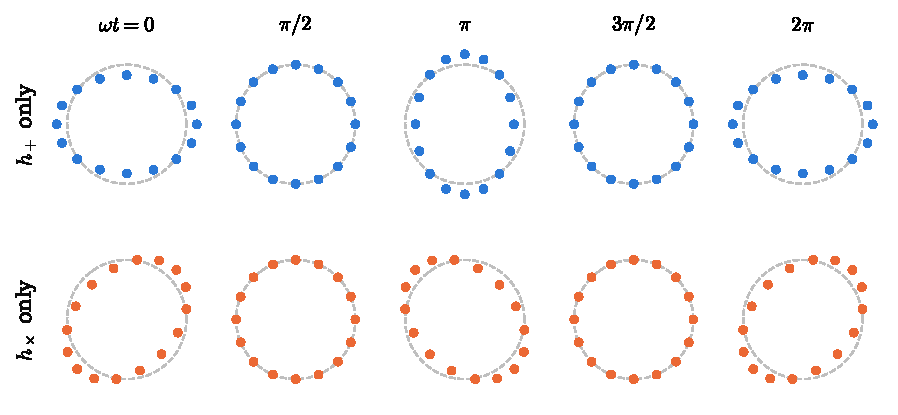
\includegraphics[width=0.9\linewidth]{figures/chT2/ring_masses.pdf}
\caption{A ring of sixteen free masses (dots) as a wave travelling out of the page passes, at five phases of one period; the dashed circle is the ring without the wave. Top row, a pure plus wave: the ring is stretched along the horizontal and squeezed along the vertical, then the reverse. Bottom row, a pure cross wave: the same breathing along the diagonals. The real amplitude is some $10^{19}$ times smaller than drawn.}
\label{T2g:fig:ring}
\end{figure}

\paragraph{Example: how large is the effect?}
For a ground-based detector with arms of $L=4$\,km and a wave of $h=10^{-21}$, \eqref{T2g:eq:displacement} gives $\delta L=\tfrac12hL=2\times10^{-18}$\,m, a few thousandths of the size of a proton. For LISA, with $L=2.5\times10^9$\,m and $h=10^{-20}$, $\delta L=\tfrac12\times10^{-20}\times2.5\times10^9\approx10^{-11}$\,m, about ten picometres. The longer the arm, the larger the displacement for the same strain, which is one reason to fly a detector in space. The other is that on the ground the seismic shaking of the Earth swamps everything below a few hertz.

\begin{pitfall}[Coordinates that do not move]
``In the TT gauge the masses do not move'' and ``the wave changes the distance between them'' are both true. The first is a statement about labels, which the TT gauge attaches to the free masses themselves. The second is the physics. Every measurable effect must be computed as a proper distance or a light travel time, as in \eqref{T2g:eq:proper}, never read off from a change of coordinates.
\end{pitfall}

\subsection{The energy a wave carries}
\label{T2g:sec:energy}

A wave that can push masses around can do work, so it carries energy. Energy in general relativity is subtle, because the gravitational field has no energy density at a single point: at any one point a freely falling observer sees no field at all. What is well defined is the energy averaged over a region several wavelengths across. This is our fourth input, imported from general relativity \cite[Sec.~1.4]{Maggiore2007}: the energy crossing unit area per unit time, for a wave in the TT gauge, is
\begin{equation}
  \mathcal F=\frac{c^3}{32\pi G}\,\big\langle\dot h^{\rm TT}_{ij}\dot h^{\rm TT}_{ij}\big\rangle
  =\frac{c^3}{16\pi G}\,\big\langle\dot h_+^2+\dot h_\times^2\big\rangle ,
  \label{T2g:eq:flux}
\end{equation}
where the angle brackets average over several periods, and the second form follows from \eqref{T2g:eq:tt}, since $h_{ij}h_{ij}=h_+^2+h_\times^2+h_\times^2+h_+^2$. Its form is that of the electromagnetic Poynting flux of a radiation field, $\varepsilon_0c\langle E^2\rangle$ with $E=-\dot A$. The flux is quadratic in the field because energy is, and it contains the time derivative because a static strain, like a static potential, carries nothing away.

\paragraph{Example: why a strain of $10^{-21}$ is a lot of energy.}
The constant in front of \eqref{T2g:eq:flux} is enormous:
\begin{align*}
  \frac{c^3}{16\pi G}
  &\eqby{1}\frac{(3.0\times10^8)^3}{16\pi\times6.67\times10^{-11}}\ \frac{\rm kg}{\rm s}
  \eqby{2}8.0\times10^{33}\ {\rm kg\,s^{-1}} .
\end{align*}
\begin{explain}
  \item $c$ in m\,s$^{-1}$ and $G$ in m$^3$\,kg$^{-1}$\,s$^{-2}$; the units combine to kg\,s$^{-1}$, which times $\dot h^2$ in s$^{-2}$ gives W\,m$^{-2}$.
  \item $2.7\times10^{25}/3.35\times10^{-9}=8.0\times10^{33}$.
\end{explain}
Take the first detected wave near its peak, $h_+=h\cos2\pi ft$ with $h\approx10^{-21}$ and $f\approx250$\,Hz. Then $\langle\dot h_+^2\rangle=\tfrac12(2\pi fh)^2=\tfrac12(1.6\times10^{-18}\,{\rm s^{-1}})^2=1.2\times10^{-36}\,{\rm s^{-2}}$, and $\mathcal F\approx8.0\times10^{33}\times1.2\times10^{-36}\approx10^{-2}$\,W\,m$^{-2}$. For a fraction of a second, the Earth received more energy per square metre in gravitational waves than it receives in light from any star in the night sky. Yet the strain was $10^{-21}$. Spacetime is stiff: the factor $c^3/G$ means a large energy flux produces only a minute deformation, and, the other way round, a measurable deformation needs a violent source.

\paragraph{Where this is used.}
The two polarisations and the factor $\tfrac12$ in $\delta L/L$ are what a detector turns into the single strain $h(t)=F_+h_++F_\times h_\times$ of \cref{T2g:sec:detector}. That strain is the signal part of the data stream $d(t)=h(t)+n(t)$ with which \cref{10b:sec:detection} begins, and the energy flux \eqref{T2g:eq:flux} drives the chirp of \cref{T2a:sec:chirp}, whose phase is what \cref{10b:sec:fisher} measures.
\section{Why radiation starts at the quadrupole}
\label{T2g:sec:quadrupole}

A radio antenna radiates because electrons slosh back and forth along it: the electric dipole moment, charge times separation, oscillates. Two black holes on an orbit look at first sight like the same thing, two ``charges'' swinging round each other, so we might expect them to radiate like a rotating dipole, at the orbital frequency. They do not. The gravitational wave of a binary comes out at \emph{twice} the orbital frequency, and it is weaker than a dipole estimate by a factor $(v/c)^2$. Both facts have one cause. The ``charge'' of gravity is mass, it has only one sign, and it is the same mass that sets the inertia of the body. As a result the two quantities that make up the monopole and the dipole of the field, the total mass and the position of the centre of mass, cannot oscillate: they are protected by conservation laws.

The question, in words: \emph{starting from the field equation of \cref{T2g:sec:wave}, which part of a moving mass distribution produces a wave far away, how large is the wave, and how much power does it carry off?} For a binary the answers are the waveform $h_+$, $h_\times$ that every template in \cref{ch:10} is built on, and the power $P_{\rm GW}$ that drives the chirp of \cref{T2a:sec:chirp}.

\subsection{The field far from a slow source}

\emph{Inputs.} We keep the inputs of \cref{T2g:sec:wave}: the weak-field metric \eqref{T2g:eq:weak} and the linearised field equation \eqref{T2g:eq:linear-einstein}, $\Box\bar h_{\mu\nu}=-(16\pi G/c^4)T_{\mu\nu}$. We add three about the source.
\begin{enumerate}[itemsep=1pt]
  \item \emph{Physical: small and slow.} The source has size $d$ and internal speeds $v\ll c$. It then changes on a time scale $d/v$, so it emits at wavelengths $\lambda\sim c\,d/v\gg d$.
  \item \emph{Physical: energy and momentum are conserved}, $\partial_\mu T^{\mu\nu}=0$, and the source is Newtonian, $T^{00}=\rho c^2$ with $\rho$ the mass density. For a binary held together by its own gravity this is true only once the energy of the gravitational field is counted as well. The full theory shows that the leading-order result derived below is unchanged by that \cite[Sec.~3.1]{Maggiore2007}.
  \item \emph{Mathematical: the retarded solution.} The solution of $\Box\psi=-4\pi s$ that contains only outgoing waves is $\psi(t,\bm x)=\int s(t-\lvert\bm x-\bm x'\rvert/c,\bm x')/\lvert\bm x-\bm x'\rvert\,\dd^3x'$, the retarded potential familiar from electrodynamics. Applied to each component of \eqref{T2g:eq:linear-einstein},
  \begin{equation}
    \bar h_{\mu\nu}(t,\bm x)=\frac{4G}{c^4}\int\frac{T_{\mu\nu}\big(t-\lvert\bm x-\bm x'\rvert/c,\ \bm x'\big)}{\lvert\bm x-\bm x'\rvert}\,\dd^3x' .
    \label{T2g:eq:retarded}
  \end{equation}
\end{enumerate}

\emph{Far away.} The detector sits at distance $r=\lvert\bm x\rvert\gg d$ in the direction $\hat{\bm n}=\bm x/r$. For a point $\bm x'$ of the source, $\lvert\bm x-\bm x'\rvert=r-\hat{\bm n}\cdot\bm x'+O(d^2/r)$. In the denominator of \eqref{T2g:eq:retarded} the correction is negligible and we write $1/r$. In the time argument it is not automatically negligible, because it multiplies a rapidly varying function:
\begin{equation}
  T_{\mu\nu}\Big(t-\frac rc+\frac{\hat{\bm n}\cdot\bm x'}{c},\bm x'\Big)
  =T_{\mu\nu}(t_r,\bm x')+\frac{\hat n_ix'_i}{c}\,\partial_tT_{\mu\nu}(t_r,\bm x')
  +\frac{\hat n_i\hat n_jx'_ix'_j}{2c^2}\,\partial_t^2T_{\mu\nu}(t_r,\bm x')+\dots,
  \label{T2g:eq:multipole}
\end{equation}
with $t_r=t-r/c$ the \newterm{retarded time}. Each term is smaller than the one before by about $(d/c)/(d/v)=v/c$: the time light takes to cross the source, divided by the time the source takes to change. This is the \newterm{multipole expansion}, and the slow-motion input says it converges quickly.

\emph{Which terms can change in time?} Apply \eqref{T2g:eq:multipole} to the $00$ component, with $T_{00}=\rho c^2$:
\begin{equation}
  \bar h_{00}=\frac{4G}{c^2r}\Big[M+\frac{\hat n_i}{c}\,\dot M_i+\frac{\hat n_i\hat n_j}{2c^2}\,\ddot M_{ij}+\dots\Big]_{t_r},
  \qquad M=\int\rho,\quad M_i=\int\rho\,x_i,\quad M_{ij}=\int\rho\,x_ix_j ,
  \label{T2g:eq:moments}
\end{equation}
where every integral is over the source at the retarded time. The three moments are the mass, the mass dipole and the second mass moment. Take them one at a time.

\emph{The monopole.} Mass conservation, the $\nu=0$ part of input 2, is the continuity equation $\partial_t\rho+\partial_k(\rho v_k)=0$. Integrated over a volume enclosing the source, the divergence becomes a flux through a surface where there is no matter, so $\dot M=0$. The first term is the static Newtonian potential $4GM/(c^2r)$ and carries no wave.

\emph{The dipole.} Using the continuity equation again,
\begin{align}
  \dot M_i
  &\eqby{1}\int x_i\,\partial_t\rho\,\dd^3x
  \eqby{2}-\int x_i\,\partial_k(\rho v_k)\,\dd^3x
  \eqby{3}\int\rho\,v_k\,\partial_kx_i\,\dd^3x
  \eqby{4}\int\rho\,v_i\,\dd^3x=P_i ,
  \label{T2g:eq:dipole}
\end{align}
\begin{explain}
  \item Differentiate under the integral; the integration region is fixed.
  \item Continuity equation.
  \item Integrate by parts; the surface term vanishes outside the source.
  \item $\partial_kx_i=\delta_{ik}$. The result is the total momentum $P_i$.
\end{explain}
Momentum conservation, the $\nu=i$ part of input 2, gives $\dot P_i=0$, so $\ddot M_i=0$: $\dot M_i$ is constant. The second term of \eqref{T2g:eq:moments} is the field of a mass whose centre moves at constant velocity, and that does not radiate either. In electromagnetism the dipole moment is $\sum q\,\bm x$, whose derivative $\sum q\,\bm v$ is not a conserved quantity, because different particles carry different charge per unit mass. In gravity every body's ``charge'' is its mass, the very quantity that sets its momentum, so the dipole is tied to the centre of mass and frozen.

\emph{The quadrupole.} Nothing stops $\ddot M_{ij}$ from oscillating. The first time-dependent term, and so the first radiating one, is the second moment of the mass. A spinning symmetric top has a constant $M_{ij}$ and stays silent; a dumbbell rotating about an axis through its middle does not, and radiates.

\begin{figure}[htbp]
\centering
\begin{tikzpicture}[scale=0.9]
  \begin{scope}
    \shade[ball color=formblue!35] (0,0) circle (0.75);
    \node[lbl] at (0,-1.35) {mass $M$};
    \node[lbl,align=center] at (0,-2.05) {conserved:\\ no wave};
  \end{scope}
  \begin{scope}[xshift=4.2cm]
    \fill[formblue] (-0.9,0.25) circle (3pt);
    \fill[formblue] (0.5,-0.25) circle (4pt);
    \draw[faint,dashed] (-0.9,0.25) -- (0.5,-0.25);
    \fill[bdryred] (0.03,-0.08) circle (1.6pt);
    \draw[vec] (0.03,-0.08) -- ++(0.9,0.55);
    \node[lbl] at (0,-1.35) {centre of mass};
    \node[lbl,align=center] at (0,-2.05) {moves uniformly:\\ no wave};
  \end{scope}
  \begin{scope}[xshift=8.6cm]
    \foreach \ang/\op in {0/1,45/0.45,90/0.2}{
      \draw[formblue,thick,opacity=\op] (\ang:0.85) -- (\ang+180:0.85);
      \fill[formblue,opacity=\op] (\ang:0.85) circle (3.5pt);
      \fill[formblue,opacity=\op] (\ang+180:0.85) circle (3.5pt);}
    \draw[->,faint] (20:1.2) arc (20:70:1.2);
    \node[lbl] at (0,-1.35) {shape $M_{ij}$};
    \node[lbl,align=center] at (0,-2.05) {changes twice\\ per turn: waves};
  \end{scope}
\end{tikzpicture}
\caption{The three lowest moments of a mass distribution. The total mass (left) cannot change. The mass dipole is the total mass times the position of the centre of mass (middle, red dot), which can only move at constant velocity. The second moment (right) describes the shape; for a rotating dumbbell, drawn at three instants an eighth of a turn apart, it returns to the same value after half a turn, so it oscillates at twice the rotation frequency.}
\label{T2g:fig:multipoles}
\end{figure}

\emph{The wave itself.} The radiation lives in the spatial components $\bar h_{ij}$. At leading order in $v/c$ we keep only the first term of \eqref{T2g:eq:multipole}, so $\bar h_{ij}=(4G/c^4r)\int T_{ij}(t_r,\bm x')\,\dd^3x'$. The integral of the stresses $T_{ij}$ is not obviously related to the mass distribution, but conservation turns it into one:
\begin{align}
  \frac{1}{c^2}\frac{\dd^2}{\dd t^2}\int T^{00}x_ix_j\,\dd^3x
  &\eqby{1}\int x_ix_j\,\partial_0\partial_0T^{00}\,\dd^3x
  \eqby{2}\int x_ix_j\,\partial_k\partial_lT^{kl}\,\dd^3x\nonumber\\
  &\eqby{3}\int T^{kl}\,\partial_k\partial_l(x_ix_j)\,\dd^3x
  \eqby{4}2\int T^{ij}\,\dd^3x .
  \label{T2g:eq:virial}
\end{align}
\begin{explain}
  \item $x^0=ct$, so $\partial_0=c^{-1}\partial_t$.
  \item From $\partial_\mu T^{\mu\nu}=0$: $\partial_0T^{00}=-\partial_kT^{k0}$ and $\partial_0T^{0k}=-\partial_lT^{lk}$, so $\partial_0\partial_0T^{00}=-\partial_k\partial_0T^{0k}=\partial_k\partial_lT^{kl}$.
  \item Integrate by parts twice; both surface terms vanish outside the source.
  \item $\partial_l(x_ix_j)=\delta_{il}x_j+x_i\delta_{jl}$ and then $\partial_k$ of that is $\delta_{il}\delta_{jk}+\delta_{ik}\delta_{jl}$; both terms give $T^{ij}$ because $T$ is symmetric.
\end{explain}
With $T^{00}=\rho c^2$ the left side is $\ddot M_{ij}$, so $\int T_{ij}=\tfrac12\ddot M_{ij}$ and $\bar h_{ij}=(2G/c^4r)\ddot M_{ij}(t_r)$. Far from the source the wave is locally a plane wave travelling along $\hat{\bm n}$, and its physical content is its TT part, obtained with the recipe of the working definition in \cref{T2g:sec:wave}: keep the components in the plane perpendicular to $\hat{\bm n}$ and remove their trace. Removing the trace means that $M_{ij}$ may as well be replaced by its traceless part, the \newterm{mass quadrupole}
\begin{equation}
  Q_{ij}=\int\rho\,\Big(x_ix_j-\tfrac13\delta_{ij}\lvert\bm x\rvert^2\Big)\dd^3x ,
  \qquad
  h_{ij}^{\rm TT}(t,\bm x)=\frac{2G}{c^4r}\,\big[\ddot Q_{ij}(t-r/c)\big]^{\rm TT} .
  \label{T2g:eq:hTT}
\end{equation}
This is the \newterm{quadrupole formula} for the wave \cite[Sec.~3.3]{Maggiore2007}. In terms of the transverse unit vectors $\bm p$, $\bm q$ and the recipe of the working definition, $h_+=\frac{G}{c^4r}\big(\ddot Q_{pp}-\ddot Q_{qq}\big)$ and $h_\times=\frac{2G}{c^4r}\ddot Q_{pq}$.

\begin{keyidea}[The quadrupole formula]
Far from a slow source, the wave is $h_{ij}^{\rm TT}=(2G/c^4r)\,[\ddot Q_{ij}(t-r/c)]^{\rm TT}$, with $Q_{ij}$ the traceless second moment of the mass. Mass and momentum conservation forbid monopole and dipole radiation, so the quadrupole is the leading term, and each further multipole is suppressed by another factor $v/c$.
\end{keyidea}

\subsection{The circular binary}

\emph{The quadrupole of a binary.} Two masses $m_1$, $m_2$ at positions $\bm x_1$, $\bm x_2$, centre of mass at rest at the origin. With $M=m_1+m_2$, the separation $\bm x=\bm x_1-\bm x_2$ and the \newterm{reduced mass} $\mu=m_1m_2/M$, the positions are $\bm x_1=(m_2/M)\bm x$ and $\bm x_2=-(m_1/M)\bm x$, and
\begin{equation}
  M_{ij}=m_1x_{1i}x_{1j}+m_2x_{2i}x_{2j}=\Big(\frac{m_1m_2^2}{M^2}+\frac{m_2m_1^2}{M^2}\Big)x_ix_j=\mu\,x_ix_j ,
\end{equation}
so the binary radiates like a single body of mass $\mu$ on the relative orbit. For a circular orbit of radius $r$ in the $xy$ plane, $\bm x=r(\cos\omega t,\sin\omega t,0)$, and Kepler's third law $\omega^2=GM/r^3$ links $\omega$ and $r$. The components we need are
\begin{align}
  M_{xx}&\eqby{1}\mu r^2\cos^2\omega t\eqby{2}\tfrac12\mu r^2(1+\cos2\omega t),\qquad
  M_{yy}\eqby{2}\tfrac12\mu r^2(1-\cos2\omega t),\qquad
  M_{xy}\eqby{2}\tfrac12\mu r^2\sin2\omega t,\nonumber\\
  \ddot M_{xx}&\eqby{3}-2\mu r^2\omega^2\cos2\omega t=-\ddot M_{yy},\qquad
  \ddot M_{xy}\eqby{3}-2\mu r^2\omega^2\sin2\omega t,
  \label{T2g:eq:Mddot}
\end{align}
and every component with a $z$ is zero or constant.
\begin{explain}
  \item $x_x=r\cos\omega t$.
  \item $\cos^2\theta=\tfrac12(1+\cos2\theta)$, $\sin^2\theta=\tfrac12(1-\cos2\theta)$, $\sin\theta\cos\theta=\tfrac12\sin2\theta$.
  \item Two time derivatives of $\cos2\omega t$ or $\sin2\omega t$ bring down $-(2\omega)^2$; the constants drop out.
\end{explain}
Everything oscillates at $2\omega$. The mass distribution of the pair, a dumbbell, looks the same after half a turn, so the wave frequency is twice the orbital one:
\begin{equation}
  f_{\rm GW}=2f_{\rm orb}=\frac{\omega}{\pi}.
  \label{T2g:eq:twice}
\end{equation}
From here on $f$ without a label means the wave frequency $f_{\rm GW}$.

\emph{The two polarisations seen from an angle.} Let the observer look at the binary from the direction $\hat{\bm n}=(0,\sin\iota,\cos\iota)$, where $\iota$ is the \newterm{inclination}, the angle between the orbital axis and the line of sight. Two transverse unit vectors are $\bm p=(1,0,0)$ and $\bm q=(0,\cos\iota,-\sin\iota)$. Then $\ddot M_{pp}=\ddot M_{xx}$, $\ddot M_{qq}=\cos^2\iota\,\ddot M_{yy}$ and $\ddot M_{pq}=\cos\iota\,\ddot M_{xy}$, because the $z$ components do not contribute. By \eqref{T2g:eq:hTT} at distance $D$,
\begin{align}
  h_+&\eqby{1}\frac{G}{c^4D}\big(\ddot M_{xx}-\cos^2\iota\,\ddot M_{yy}\big)
  \eqby{2}-\frac{4G\mu r^2\omega^2}{c^4D}\,\frac{1+\cos^2\iota}{2}\,\cos2\omega t_r,\nonumber\\
  h_\times&\eqby{1}\frac{2G}{c^4D}\cos\iota\,\ddot M_{xy}
  \eqby{2}-\frac{4G\mu r^2\omega^2}{c^4D}\,\cos\iota\,\sin2\omega t_r .
  \label{T2g:eq:hpc}
\end{align}
\begin{explain}
  \item The recipe $h_+=\frac{G}{c^4D}(\ddot M_{pp}-\ddot M_{qq})$, $h_\times=\frac{2G}{c^4D}\ddot M_{pq}$, with $M$ in place of $Q$ since their difference is a multiple of $\delta_{ij}$, which the TT recipe removes.
  \item Insert \eqref{T2g:eq:Mddot}: $\ddot M_{xx}-\cos^2\iota\,\ddot M_{yy}=-2\mu r^2\omega^2(1+\cos^2\iota)\cos2\omega t$.
\end{explain}
Seen face on ($\iota=0$) the two polarisations have equal size and are a quarter cycle apart: the wave is circularly polarised, as the rotating dumbbell suggests. Seen edge on ($\iota=90^\circ$) only $h_+$ is left, at half the face-on size: the dumbbell seen from the side only grows and shrinks.

\emph{The amplitude as a function of the wave frequency.} Kepler's law gives $r^2\omega^2=(GM)^{2/3}\omega^{2/3}$, and $\omega=\pi f$. So the common factor in \eqref{T2g:eq:hpc} is
\begin{align}
  A\equiv\frac{4G\mu r^2\omega^2}{c^4D}
  &\eqby{1}\frac{4G\mu(GM)^{2/3}(\pi f)^{2/3}}{c^4D}
  \eqby{2}\frac{4(G\mathcal M)^{5/3}(\pi f)^{2/3}}{c^4D},
  \qquad \mathcal M\equiv\mu^{3/5}M^{2/5}=\frac{(m_1m_2)^{3/5}}{(m_1+m_2)^{1/5}} .
  \label{T2g:eq:amp}
\end{align}
\begin{explain}
  \item $r=(GM/\omega^2)^{1/3}$, so $r^2\omega^2=(GM)^{2/3}\omega^{2/3}$.
  \item $G\mu\,G^{2/3}M^{2/3}=G^{5/3}\mu M^{2/3}$, and $\mu M^{2/3}=(\mu^{3/5}M^{2/5})^{5/3}=\mathcal M^{5/3}$.
\end{explain}
The masses enter only through the \newterm{chirp mass} $\mathcal M$; \cref{T2a:sec:chirp} finds the same combination in the rate of the chirp. This amplitude is the one used for the Fourier-domain waveform in \cref{T2a:sec:spa}, where it becomes the constant $\mathcal A$ of \eqref{T2a:eq:hf}; it is the time-domain amplitude quoted by Eda et al.\ \cite[eq.~(21)]{Eda2015}.

\paragraph{Example: the size of the wave from a known source.}
For a GW150914-like binary, $\mathcal M=28\,M_\odot$, so $G\mathcal M/c^3=28\times4.93\,\mu{\rm s}=1.38\times10^{-4}$\,s, at $D=410$\,Mpc$\,=1.27\times10^{25}$\,m and $f=250$\,Hz. Write \eqref{T2g:eq:amp} with the masses as times, $A=4(G\mathcal M/c^3)^{5/3}(\pi f)^{2/3}\,c/D$:
\begin{align*}
  A&\eqby{1}4\times\big(1.38\times10^{-4}\big)^{5/3}\times(785)^{2/3}\times\frac{3.0\times10^8}{1.27\times10^{25}}
  \eqby{2}4\times3.7\times10^{-7}\times85\times2.4\times10^{-17}
  \approx3\times10^{-21} .
\end{align*}
\begin{explain}
  \item $(G\mathcal M)^{5/3}/c^4=(G\mathcal M/c^3)^{5/3}c^5/c^4$, and $\pi\times250=785$\,s$^{-1}$.
  \item $10^{-3.86\times5/3}=10^{-6.43}=3.7\times10^{-7}$; $785^{2/3}=85$; $c/D=2.4\times10^{-17}$\,s$^{-1}$.
\end{explain}
This is the strain of order $10^{-21}$ used in \cref{T2g:sec:energy}. For the intermediate mass-ratio benchmark of \cref{T2a:sec:chirp} ($\mathcal M\approx19\,M_\odot$) at $75$\,Mpc and $f=20$\,mHz the same steps give $A\approx1.6\times10^{-23}$. It is the millions of cycles, not the instantaneous size, that make such a source detectable.

\subsection{The power}

\emph{From the flux.} The power leaving the binary is the flux \eqref{T2g:eq:flux} integrated over a sphere of radius $D$. Over one period, $\langle\sin^2\rangle=\langle\cos^2\rangle=\tfrac12$, and each time derivative of \eqref{T2g:eq:hpc} brings down $2\omega$, so $\langle\dot h_+^2+\dot h_\times^2\rangle=\tfrac12(2\omega A)^2\big[\tfrac14(1+\cos^2\iota)^2+\cos^2\iota\big]$. The bracket is the angular pattern of the radiation (\cref{T2g:fig:pattern}). It does not depend on the observer's azimuth, because a circular orbit seen from a different azimuth is the same orbit seen at a different moment. With $x=\cos\iota$ and $\dd\Omega=\dd\phi\,\dd x$,
\begin{align}
  P_{\rm GW}
  &\eqby{1}\int\frac{c^3}{16\pi G}\big\langle\dot h_+^2+\dot h_\times^2\big\rangle D^2\,\dd\Omega
  \eqby{2}\frac{c^3D^2}{16\pi G}\cdot2\omega^2A^2\cdot2\pi\int_{-1}^{1}\Big[\frac{(1+x^2)^2}{4}+x^2\Big]\dd x\nonumber\\
  &\eqby{3}\frac{c^3D^2}{16\pi G}\cdot2\omega^2A^2\cdot\frac{16\pi}{5}
  \eqby{4}\frac25\,\frac{c^3}{G}\,\omega^2(DA)^2
  \eqby{5}\frac{32}{5}\,\frac{G}{c^5}\,\mu^2r^4\omega^6 .
  \label{T2g:eq:power-binary}
\end{align}
\begin{explain}
  \item Flux times area, summed over all directions.
  \item $\tfrac12(2\omega A)^2=2\omega^2A^2$; the $\phi$ integral gives $2\pi$.
  \item $\int_{-1}^1(1+x^2)^2\dd x=2+\tfrac43+\tfrac25=\tfrac{56}{15}$ and $\int_{-1}^1x^2\dd x=\tfrac23$, so the integral is $\tfrac14\cdot\tfrac{56}{15}+\tfrac23=\tfrac{14}{15}+\tfrac{10}{15}=\tfrac85$, and $2\pi\cdot\tfrac85=\tfrac{16\pi}5$.
  \item $\frac{2\cdot16\pi}{16\pi\cdot5}=\frac25$.
  \item $DA=4G\mu r^2\omega^2/c^4$ from \eqref{T2g:eq:amp}, so $(DA)^2=16G^2\mu^2r^4\omega^4/c^8$; then $\tfrac25\cdot16=\tfrac{32}5$, $c^3/c^8=c^{-5}$ and $G^2/G=G$.
\end{explain}
The angular integral $\int[\tfrac14(1+x^2)^2+x^2]\dd\Omega=16\pi/5$ is worth remembering; divided by $4\pi$ it is the average $\tfrac45$ that reappears in the sky-averaged waveform of \cref{T2a:sec:spa}.

\emph{From the quadrupole directly.} The same integral can be done once and for all for any source. Insert \eqref{T2g:eq:hTT} into \eqref{T2g:eq:flux}. The TT recipe is a projection, applying it twice changes nothing, and for a traceless symmetric matrix it gives
\begin{align}
  [\dddot Q]^{\rm TT}_{ij}[\dddot Q]^{\rm TT}_{ij}
  &\eqby{1}\dddot Q_{ij}\dddot Q_{ij}-2\,\hat n_i\dddot Q_{ik}\dddot Q_{kj}\hat n_j+\tfrac12\big(\hat n_i\dddot Q_{ij}\hat n_j\big)^2,\nonumber\\
  \frac{1}{4\pi}\int[\dddot Q]^{\rm TT}_{ij}[\dddot Q]^{\rm TT}_{ij}\,\dd\Omega
  &\eqby{2}\dddot Q_{ij}\dddot Q_{ij}\Big(1-\frac23+\frac{2}{15}\cdot\frac12\Big)
  =\frac25\,\dddot Q_{ij}\dddot Q_{ij},\nonumber\\
  P_{\rm GW}
  &\eqby{3}\frac{c^3r^2}{32\pi G}\Big(\frac{2G}{c^4r}\Big)^2\cdot4\pi\cdot\frac25\,\big\langle\dddot Q_{ij}\dddot Q_{ij}\big\rangle
  =\frac{G}{5c^5}\,\big\langle\dddot Q_{ij}\dddot Q_{ij}\big\rangle .
  \label{T2a:eq:quadrupole}
\end{align}
\begin{explain}
  \item With the projector $P_{ij}=\delta_{ij}-\hat n_i\hat n_j$ onto the transverse plane, the recipe is $[Q]^{\rm TT}=PQP-\tfrac12P\,\mathrm{tr}(PQ)$. Squaring and taking the trace, with $P^2=P$ and $\mathrm{tr}P=2$, gives $\mathrm{tr}(PQPQ)-\mathrm{tr}(PQ)^2+\tfrac14\cdot2\,\mathrm{tr}(PQ)^2=\mathrm{tr}(PQPQ)-\tfrac12\mathrm{tr}(PQ)^2$. Multiplying out $P=\mathbb 1-\hat{\bm n}\hat{\bm n}^{\mathsf T}$ gives $\mathrm{tr}(PQPQ)=\mathrm{tr}Q^2-2\,\hat{\bm n}\cdot Q^2\hat{\bm n}+(\hat{\bm n}\cdot Q\hat{\bm n})^2$, and $\mathrm{tr}(PQ)=-\hat{\bm n}\cdot Q\hat{\bm n}$ because $\mathrm{tr}\,Q=0$.
  \item Average over directions with $\langle\hat n_i\hat n_j\rangle=\tfrac13\delta_{ij}$ and $\langle\hat n_i\hat n_j\hat n_k\hat n_l\rangle=\tfrac1{15}(\delta_{ij}\delta_{kl}+\delta_{ik}\delta_{jl}+\delta_{il}\delta_{jk})$; for a traceless symmetric $Q$ the second gives $\langle(\hat{\bm n}\cdot Q\hat{\bm n})^2\rangle=\tfrac{2}{15}\mathrm{tr}Q^2$.
  \item The flux \eqref{T2g:eq:flux} with $\dot h^{\rm TT}=(2G/c^4r)[\dddot Q]^{\rm TT}$, times $r^2$, integrated over $4\pi$; $\frac{c^3}{32\pi G}\cdot\frac{4G^2}{c^8}\cdot4\pi\cdot\frac25=\frac{G}{5c^5}$.
\end{explain}
For the binary, the third derivatives of \eqref{T2g:eq:Mddot} are $\dddot Q_{xx}=-\dddot Q_{yy}=4\mu r^2\omega^3\sin2\omega t$ and $\dddot Q_{xy}=-4\mu r^2\omega^3\cos2\omega t$, so
\begin{equation}
  \dddot Q_{ij}\dddot Q_{ij}=\dddot Q_{xx}^2+\dddot Q_{yy}^2+2\dddot Q_{xy}^2=(4\mu r^2\omega^3)^2\big(2\sin^2+2\cos^2\big)(2\omega t)=32\,\mu^2r^4\omega^6 ,
  \label{T2a:eq:Qddd}
\end{equation}
and \eqref{T2a:eq:quadrupole} gives $P_{\rm GW}=\tfrac{32}{5}(G/c^5)\mu^2r^4\omega^6$ again \cite[Sec.~4.1]{Maggiore2007}. Two routes, one answer: the first summed the radiation over directions by hand, the second did the same sum for a general traceless matrix.

\begin{figure}[htbp]
\centering
\begin{tikzpicture}[scale=1.0]
  \draw[faint] (-2.8,0) -- (2.8,0);
  \node[lbl,faint,anchor=south east] at (-2.85,0.05) {orbital plane};
  \draw[faint,->] (0,-2.7) -- (0,2.9) node[above,lbl] {orbital axis};
  \draw[formblue,thick,domain=0:360,samples=181,smooth,variable=\t]
    plot ({2.4*((1+cos(\t)^2)^2/4+cos(\t)^2)/2*sin(\t)},{2.4*((1+cos(\t)^2)^2/4+cos(\t)^2)/2*cos(\t)});
  \draw[fibreorange,thick,dashed,domain=0:360,samples=181,smooth,variable=\t]
    plot ({2.4*(1+cos(\t)^2)/2*sin(\t)},{2.4*(1+cos(\t)^2)/2*cos(\t)});
  \draw[tangentgreen,thick,dotted,domain=0:360,samples=181,smooth,variable=\t]
    plot ({2.4*abs(cos(\t))*sin(\t)},{2.4*abs(cos(\t))*cos(\t)});
  \fill[black] (-0.12,0) circle (1.5pt); \fill[black] (0.12,0) circle (1.5pt);
  \draw[faint] (0,0) -- (52:2.4);
  \node[lbl] at (64:1.3) {$\iota$};
  \draw[faint,->] (90:0.9) arc (90:52:0.9);
  \node[lbl,anchor=west,align=left,formblue] at (3.0,1.9) {power per solid angle,\\ $\tfrac14(1+\cos^2\iota)^2+\cos^2\iota$};
  \node[lbl,anchor=west,align=left,fibreorange] at (3.0,0.6) {$h_+$ amplitude,\\ $\tfrac12(1+\cos^2\iota)$};
  \node[lbl,anchor=west,align=left,tangentgreen!70!black] at (3.0,-0.7) {$h_\times$ amplitude,\\ $\lvert\cos\iota\rvert$};
\end{tikzpicture}
\caption{How a circular binary radiates in different directions, in units of the face-on value; the distance from the centre along a direction at angle $\iota$ from the orbital axis is the quantity named on the right. Along the axis both polarisations are full size and the power is largest. In the orbital plane $h_\times$ vanishes, $h_+$ is halved, and the power per solid angle drops from $\tfrac14\cdot2^2+1=2$ to $\tfrac14$, an eighth of its value on the axis.}
\label{T2g:fig:pattern}
\end{figure}

\paragraph{Example: how much weaker than a dipole?}
Suppose, against the conservation laws, that a binary could radiate like an electric dipole. Larmor's formula, $P=q^2a^2/(6\pi\varepsilon_0c^3)$, with $q^2/(4\pi\varepsilon_0)$ replaced by $G\mu^2$ and the acceleration $a=r\omega^2$, would give $P_{\rm dip}\sim G\mu^2r^2\omega^4/c^3$. The quadrupole power is $P_{\rm GW}\sim G\mu^2r^4\omega^6/c^5$, so
\begin{equation*}
  \frac{P_{\rm GW}}{P_{\rm dip}}\sim\frac{r^2\omega^2}{c^2}=\frac{v^2}{c^2}.
\end{equation*}
Quadrupole radiation is one power of $(v/c)^2$ weaker than dipole radiation would be. In theories of gravity in which bodies carry an extra ``charge'' that is not proportional to their mass, dipole radiation does appear, and because it is relatively stronger at low speeds, it shows up at low frequency. \Cref{T2g:sec:pn} shows that it enters the phase of the wave as the power $f^{-7/3}$.

\paragraph{Where this is used.}
The amplitude \eqref{T2g:eq:amp} and its dependence on the inclination \eqref{T2g:eq:hpc} set the size of every template in \cref{ch:10}: through the constant $\mathcal A$ of \eqref{T2a:eq:hf} they fix the signal-to-noise ratio of \cref{10b:sec:matched-filter}, and through the factor $\tfrac45$ they enter the sky-averaged forecasts of \cref{10b:sec:forecast}. The power \eqref{T2g:eq:power-binary} drives the chirp of \cref{T2a:sec:chirp}, whose phase is what \cref{10b:sec:fisher} measures.
\section{How a detector turns a wave into one number}
\label{T2g:sec:detector}

A wave arrives with two polarisations, $h_+(t)$ and $h_\times(t)$, defined with respect to axes in the plane perpendicular to its direction of travel (\cref{T2g:sec:wave}). A detector records one time series. LIGO records the difference between the lengths of its two arms, read from the interference of laser light that has run up and down each of them; LISA does the same with laser links between spacecraft millions of kilometres apart. Every likelihood in \cref{ch:10} compares that one recorded number with a template, so we need the exact rule that maps $(h_+,h_\times)$ onto it.

The questions, in words: \emph{how does a change in the light travel time along one arm follow from $h_{ij}$? How do two arms combine into one strain? How strongly does the result depend on where the source sits on the sky and how its orbit is turned? And what changes when the arm is so long that the wave changes while the light is still in flight?} The answers produce three numbers that appear without explanation in most papers: the $\tfrac45$ of the inclination average, the $\tfrac15$ of the sky average, and LISA's $\tfrac{3}{10}$, together with the transfer frequency $f_*=c/(2\pi L)$.

\subsection{One arm: the light travel time}

\emph{The simplest case first.} Put one free mass at the origin and one at $x=L$, the arm along $x$, and let a wave travel along $z$ with a wavelength much longer than $L$, so that $h_{xx}=h_+$ is the same along the whole arm while the light is in flight. Light moves on $\dd s^2=0$. Along the arm only $\dd t$ and $\dd x$ change, so with the TT metric
\begin{align}
  0&\eqby{1}-c^2\dd t^2+(1+h_{xx})\,\dd x^2
  \;\Rightarrow\;
  c\,\dd t\eqby{2}\sqrt{1+h_{xx}}\,\dd x\eqby{3}\Big(1+\tfrac12h_{xx}\Big)\dd x,\nonumber\\
  T_{\rm round}&\eqby{4}\frac{2L}{c}\Big(1+\tfrac12h_{xx}\Big),
  \qquad
  \frac{\delta T_{\rm round}}{2L/c}=\tfrac12h_{xx}.
  \label{T2g:eq:arm}
\end{align}
\begin{explain}
  \item The TT line element \eqref{T2g:eq:tt} along the $x$ axis, with $\dd y=\dd z=0$.
  \item Solve for $c\,\dd t$.
  \item $\sqrt{1+\epsilon}=1+\tfrac12\epsilon$ to first order.
  \item Integrate from $0$ to $L$ and back. The end masses keep their TT coordinates (\cref{T2g:sec:free-masses}), so the coordinate length is $L$ both ways.
\end{explain}
The light takes longer exactly as if the arm had grown by $\delta L/L=\tfrac12h_{xx}$, which is the proper-distance result \eqref{T2g:eq:displacement} again: a light clock and a ruler agree. For an arm along any unit vector $\hat{\bm a}$, the same steps give $\delta L/L=\tfrac12h_{ij}\hat a_i\hat a_j$, written $\tfrac12h_{aa}$ for short.

\emph{Two arms.} A Michelson interferometer sends light along two arms $\hat{\bm u}$ and $\hat{\bm v}$ of equal length and compares the return times. Common changes cancel; the difference survives. The strain the instrument reports is the length difference divided by the arm length \cite[eq.~(5)]{LIGOGuide2020}, \cite[eq.~(11)]{BarackCutler2004}:
\begin{equation}
  h(t)\equiv\frac{\delta L_u-\delta L_v}{L}=\tfrac12\big(h_{uu}-h_{vv}\big)=D_{ij}h_{ij},
  \qquad D_{ij}\equiv\tfrac12\big(\hat u_i\hat u_j-\hat v_i\hat v_j\big).
  \label{T2g:eq:michelson}
\end{equation}
The matrix $D$, the \newterm{detector tensor}, is all the geometry of the instrument that matters while the arms are short compared with the wavelength. For a wave of plus polarisation coming straight down onto a right-angle detector with arms along $x$ and $y$, $h_{uu}=h_+$ and $h_{vv}=-h_+$, so $h=h_+$: one arm grows while the other shrinks, and the two effects add in the difference. That is why the interferometer has two arms at right angles.

\begin{figure}[htbp]
\centering
\begin{tikzpicture}[scale=1.0]
  \fill[softgray!40] (-0.25,-0.25) rectangle (0.25,0.25);
  \draw[thick] (-0.3,0.3) -- (0.3,-0.3);
  \node[lbl,anchor=north east] at (-0.3,-0.3) {beam splitter};
  \fill[formblue] (4.6,-0.35) rectangle (4.75,0.35);
  \fill[formblue] (-0.35,3.4) rectangle (0.35,3.55);
  \node[lbl,anchor=west] at (4.85,0) {mass at $L\hat{\bm u}$};
  \node[lbl,anchor=south] at (0,3.6) {mass at $L\hat{\bm v}$};
  \draw[bdryred,thick] (0.3,0.06) -- (4.6,0.06);
  \draw[bdryred,thick,<-] (0.3,-0.06) -- (4.6,-0.06);
  \draw[bdryred,thick] (0.06,0.3) -- (0.06,3.4);
  \draw[bdryred,thick,<-] (-0.06,0.3) -- (-0.06,3.4);
  \draw[fibreorange,thick] (-2.6,0) -- (-0.3,0);
  \node[lbl,anchor=south] at (-1.8,0.05) {laser};
  \draw[faint] (0,-0.3) -- (0,-1.6);
  \node[lbl,anchor=north] at (0,-1.6) {photodetector: $\delta L_u-\delta L_v$};
  \draw[faint,dashed] (2.3,1.7) ellipse (0.75 and 0.55);
  \node[lbl,align=center] at (2.3,1.7) {$h_+>0$};
  \draw[vec] (3.25,1.7) -- (3.65,1.7);
  \draw[vec] (2.3,1.1) -- (2.3,1.35);
\end{tikzpicture}
\caption{A Michelson interferometer. Laser light is split, runs along two perpendicular arms to free masses (blue) and back, and the two beams are recombined. The recombined light measures the difference of the two round-trip times. A plus wave arriving from above, at the instant drawn, lengthens the horizontal arm and shortens the vertical one (small ellipse), so the two changes add up in the difference.}
\label{T2g:fig:michelson}
\end{figure}

\subsection{Antenna patterns: where on the sky, and how turned}

\emph{The general rule.} Let the wave come from the direction $\hat{\bm n}$ (so it travels along $-\hat{\bm n}$), and let $\bm p$, $\bm q$ be the axes in the transverse plane with respect to which $h_+$ and $h_\times$ are defined. By \eqref{T2g:eq:tt} the wave is $h_{ij}=h_+e^+_{ij}+h_\times e^\times_{ij}$ with $e^+=\bm p\bm p^{\mathsf T}-\bm q\bm q^{\mathsf T}$ and $e^\times=\bm p\bm q^{\mathsf T}+\bm q\bm p^{\mathsf T}$. Inserting it in \eqref{T2g:eq:michelson},
\begin{equation}
  h(t)=F_+\,h_+(t)+F_\times\,h_\times(t),\qquad F_A=D_{ij}\,e^A_{ij}\quad(A=+,\times),
  \label{T2g:eq:response}
\end{equation}
the form used for every detector \cite[eq.~(24)]{LIGOGuide2020}.

\begin{workdef}[antenna pattern functions]
$F_+$ and $F_\times$ are the weights with which a detector adds the two polarisations of a wave into its one output, $h=F_+h_++F_\times h_\times$ \unpack{numbers between $-1$ and $1$, fixed by the arm directions, the source direction and the orientation of the polarisation axes}. \emph{Operationally:} $F_A=D_{ij}e^A_{ij}$ with the detector tensor $D=\tfrac12(\hat{\bm u}\hat{\bm u}^{\mathsf T}-\hat{\bm v}\hat{\bm v}^{\mathsf T})$.
\end{workdef}

\emph{A right-angle detector.} Take arms along $x$ and $y$ and a source at polar angle $\theta$ and azimuth $\phi$ in the detector's frame. Choose first the natural transverse axes, $\bm p_0=\hat{\bm\theta}=(\cos\theta\cos\phi,\cos\theta\sin\phi,-\sin\theta)$ and $\bm q_0=\hat{\bm\phi}=(-\sin\phi,\cos\phi,0)$. With $D=\tfrac12\mathrm{diag}(1,-1,0)$,
\begin{align}
  F_+^0&\eqby{1}\tfrac12\big(p_x^2-q_x^2-p_y^2+q_y^2\big)
  \eqby{2}\tfrac12\big(\cos^2\theta\cos^2\phi-\sin^2\phi-\cos^2\theta\sin^2\phi+\cos^2\phi\big)\nonumber\\
  &\eqby{3}\tfrac12(1+\cos^2\theta)\cos2\phi,\nonumber\\
  F_\times^0&\eqby{1}p_xq_x-p_yq_y
  \eqby{2}-\cos\theta\cos\phi\sin\phi-\cos\theta\sin\phi\cos\phi
  \eqby{3}-\cos\theta\sin2\phi .
\end{align}
\begin{explain}
  \item $D_{ij}e^A_{ij}=\tfrac12(e^A_{xx}-e^A_{yy})$, with $e^+_{xx}=p_x^2-q_x^2$ and $e^\times_{xx}=2p_xq_x$.
  \item Insert the components of $\bm p_0$ and $\bm q_0$.
  \item $\cos^2\phi-\sin^2\phi=\cos2\phi$ and $2\sin\phi\cos\phi=\sin2\phi$.
\end{explain}
If the wave's own axes are turned by an angle $\psi$, the \newterm{polarisation angle}, from $(\bm p_0,\bm q_0)$, the rule \eqref{T2g:eq:rotate} for turning axes rewrites the wave in the $(\bm p_0,\bm q_0)$ frame as $h_+\cos2\psi-h_\times\sin2\psi$ and $h_+\sin2\psi+h_\times\cos2\psi$. Collecting the coefficients of $h_+$ and $h_\times$,
\begin{equation}
\begin{aligned}
  F_+&=\tfrac12(1+\cos^2\theta)\cos2\phi\cos2\psi-\cos\theta\sin2\phi\sin2\psi,\\
  F_\times&=-\tfrac12(1+\cos^2\theta)\cos2\phi\sin2\psi-\cos\theta\sin2\phi\cos2\psi,
\end{aligned}
  \label{T2g:eq:Fplus}
\end{equation}
which is \cite[eq.~(6)]{Robson2019} and \cite[eq.~(15a)]{BarackCutler2004}; their $F_\times$ has the opposite overall sign, a matter of which way $\psi$ is counted, which no average or signal-to-noise ratio can see. The detector is deaf in four directions in its own plane, $\theta=90^\circ$ and $\phi=45^\circ,135^\circ,\dots$, along the bisectors of the arms, where both arms are stretched equally. It is most sensitive straight overhead. \Cref{T2g:fig:antenna} maps $F_+^2+F_\times^2$, which does not depend on $\psi$.

\begin{figure}[htbp]
\centering
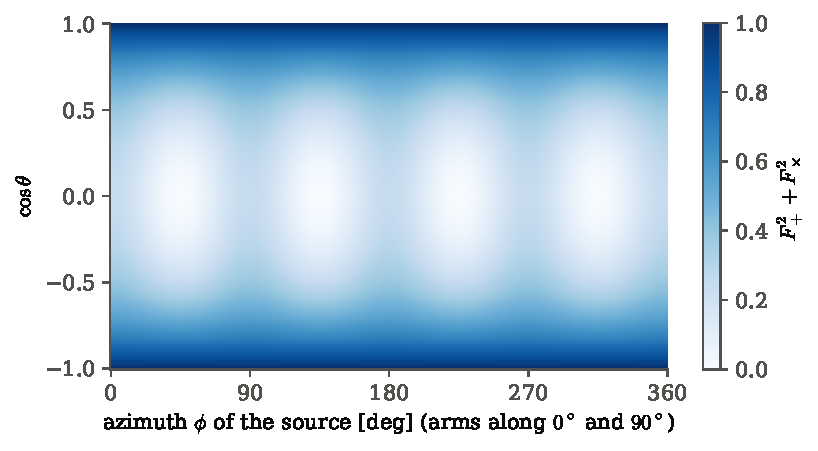
\includegraphics[width=0.78\linewidth]{figures/chT2/antenna_pattern.pdf}
\caption{The sensitivity of a right-angle interferometer over the sky, $F_+^2+F_\times^2$, as a function of the source's azimuth and of the cosine of its polar angle. It is largest above and below the detector ($\cos\theta=\pm1$), and drops to zero at four points in the plane of the arms ($\cos\theta=0$, $\phi=45^\circ$, $135^\circ$, $225^\circ$, $315^\circ$), where the wave stretches both arms equally.}
\label{T2g:fig:antenna}
\end{figure}

\paragraph{Example: a source overhead and a source in the plane of the arms.}
For a source straight overhead, $\theta=0$, \eqref{T2g:eq:Fplus} gives
\begin{align*}
  F_+&\eqby{1}\cos2\phi\cos2\psi-\sin2\phi\sin2\psi\eqby{2}\cos(2\phi+2\psi),\\
  F_\times&\eqby{1}-\cos2\phi\sin2\psi-\sin2\phi\cos2\psi\eqby{2}-\sin(2\phi+2\psi),
\end{align*}
\begin{explain}
  \item $\cos\theta=1$, so $\tfrac12(1+\cos^2\theta)=1$.
  \item The addition rules for $\cos(a+b)$ and $\sin(a+b)$.
\end{explain}
so $F_+^2+F_\times^2=1$ whatever the orientation: overhead, the detector catches the full wave, and turning the polarisation axes only moves the signal from one polarisation to the other. For a source in the plane of the arms, in the direction of the $x$ arm ($\theta=90^\circ$, $\phi=0$), we get $F_+=\tfrac12\cos2\psi$ and $F_\times=-\tfrac12\sin2\psi$, so $F_+^2+F_\times^2=\tfrac14$: the wave travels along the $x$ arm, which it cannot stretch because the wave is transverse, and only the $y$ arm responds, with its weight $\tfrac12$ in the difference \eqref{T2g:eq:michelson}.

\emph{The sky and polarisation average.} For forecasts the source's position and orientation are not known, so the response is averaged over all of them, with the source direction uniform on the sphere and $\psi$ uniform. Take $\langle F_+^2\rangle$ in three steps, one angle at a time:
\begin{align}
  \big\langle F_+^2\big\rangle_\psi
  &\eqby{1}\tfrac12\Big[\tfrac14(1+\cos^2\theta)^2\cos^22\phi+\cos^2\theta\sin^22\phi\Big],\nonumber\\
  \big\langle F_+^2\big\rangle_{\psi,\phi}
  &\eqby{2}\tfrac14\Big[\tfrac14(1+\cos^2\theta)^2+\cos^2\theta\Big],\nonumber\\
  \big\langle F_+^2\big\rangle
  &\eqby{3}\tfrac14\Big[\tfrac14\cdot\tfrac{28}{15}+\tfrac13\Big]=\tfrac14\cdot\tfrac{12}{15}=\tfrac15 .
  \label{T2g:eq:one-fifth}
\end{align}
\begin{explain}
  \item Square \eqref{T2g:eq:Fplus}; over a full turn of $\psi$, $\langle\cos^22\psi\rangle=\langle\sin^22\psi\rangle=\tfrac12$ and $\langle\cos2\psi\sin2\psi\rangle=0$, so the cross term drops.
  \item The same averages over $\phi$.
  \item A direction uniform on the sphere has $x=\cos\theta$ uniform on $[-1,1]$, so $\langle(1+x^2)^2\rangle=\tfrac12\int_{-1}^1(1+2x^2+x^4)\dd x=1+\tfrac13+\tfrac15=\tfrac{28}{15}$ and $\langle x^2\rangle=\tfrac13$.
\end{explain}
The same steps give $\langle F_\times^2\rangle=\tfrac15$, and $\langle F_+F_\times\rangle=0$. This is the $\tfrac15$ of \cite[eq.~(7)]{Robson2019}. The bracket in the second line is the same function $\tfrac14(1+\cos^2)^2+\cos^2$ that described the radiation pattern of a binary in \cref{T2g:sec:quadrupole}: a detector receives from each direction in the same pattern as a rotating quadrupole emits into it, because both are the TT part of a quadrupolar tensor.

\emph{The inclination average.} The source has its own orientation. By \eqref{T2g:eq:hpc} a circular binary at inclination $\iota$ has $h_+=A\tfrac12(1+\cos^2\iota)\cos\Phi$ and $h_\times=A\cos\iota\sin\Phi$ (up to an overall sign), where $\Phi$ is the wave's phase. Averaged over $\psi$, $F_+^2$ and $F_\times^2$ have the same mean and no correlation, so the mean squared signal is $\langle F_+^2\rangle A^2[\tfrac14(1+\cos^2\iota)^2+\cos^2\iota]$, and averaging over orientations of the orbit, $x=\cos\iota$ uniform,
\begin{equation}
  \Big\langle\tfrac14(1+x^2)^2+x^2\Big\rangle_x=\tfrac14\cdot\tfrac{28}{15}+\tfrac13=\tfrac{7}{15}+\tfrac{5}{15}=\tfrac45 .
  \label{T2g:eq:four-fifths}
\end{equation}
This is the $\tfrac45$ in the sky-averaged waveform $\tilde h=\sqrt{4/5}\,\mathcal Af^{-7/6}e^{-i\Psi}$ of \cite[eq.~(44)]{Kim2023} and \cite[eq.~(16)]{Robson2019}, and divided into $16\pi/5$ over $4\pi$ it is the same angular integral that gave the binary's total power. For a ground-based detector the two averages combine to $\tfrac45\cdot\tfrac15=\tfrac4{25}$ in power, $\tfrac25$ in amplitude, the factor quoted in the LIGO literature.

\subsection{LISA at low frequency: \texorpdfstring{$60^\circ$}{60 degree} arms and two channels}

LISA's three spacecraft form an equilateral triangle (\cref{T2a:fig:lisa-triangle}), so two arms meeting at a spacecraft make $60^\circ$, not $90^\circ$. \emph{How much does that cost?} Let $\hat{\bm e}_1$ be the unit vector along the bisector of the two arms and $\hat{\bm e}_2$ the perpendicular one in their plane, so that with $\alpha=60^\circ$ the opening angle,
\begin{align}
  \hat{\bm u}&=\cos\tfrac\alpha2\,\hat{\bm e}_1+\sin\tfrac\alpha2\,\hat{\bm e}_2,\qquad
  \hat{\bm v}=\cos\tfrac\alpha2\,\hat{\bm e}_1-\sin\tfrac\alpha2\,\hat{\bm e}_2,\nonumber\\
  2D=\hat{\bm u}\hat{\bm u}^{\mathsf T}-\hat{\bm v}\hat{\bm v}^{\mathsf T}
  &\eqby{1}2\cos\tfrac\alpha2\sin\tfrac\alpha2\big(\hat{\bm e}_1\hat{\bm e}_2^{\mathsf T}+\hat{\bm e}_2\hat{\bm e}_1^{\mathsf T}\big)
  \eqby{2}\sin\alpha\,\big(\hat{\bm e}_1\hat{\bm e}_2^{\mathsf T}+\hat{\bm e}_2\hat{\bm e}_1^{\mathsf T}\big).
  \label{T2g:eq:sixty}
\end{align}
\begin{explain}
  \item Multiply out: the $\hat{\bm e}_1\hat{\bm e}_1^{\mathsf T}$ and $\hat{\bm e}_2\hat{\bm e}_2^{\mathsf T}$ terms are the same in both and cancel; the mixed terms add.
  \item $2\sin\tfrac\alpha2\cos\tfrac\alpha2=\sin\alpha$.
\end{explain}
For $\alpha=90^\circ$ the bracket is the detector tensor of a right-angle interferometer whose arms lie along $(\hat{\bm e}_1\pm\hat{\bm e}_2)/\sqrt2$. So a $60^\circ$ interferometer is a right-angle interferometer, turned by $45^\circ$ relative to its bisector, with every response multiplied by $\sin60^\circ=\sqrt3/2$: the factor in \cite[eq.~(14)]{BarackCutler2004}. Turning does not change a sky average, so each $60^\circ$ channel has $\langle F_+^2\rangle=\tfrac34\cdot\tfrac15=\tfrac{3}{20}$. The three arms of the triangle provide two such independent channels at low frequency, the second equivalent to the first turned by $45^\circ$ \cite[eqs.~(12), (15b)]{BarackCutler2004}, and the sensitivity-curve literature sums them: $R=2\times\tfrac3{20}=\tfrac3{10}$ \cite[eqs.~(8)--(9)]{Robson2019}. The script \pyname{13_lisa_response.py} checks all of these averages by quadrature over the sky and $\psi$ and finds $\TwFpNinety$ and $\TwFxNinety$ for a right-angle detector, $\TwFpSixty$ for one $60^\circ$ channel, $\TwInclAvg$ for the inclination average and $\TwFluxInt\,\pi$ for the angular integral of the binary's power.

\begin{figure}[htbp]
\centering
\begin{tikzpicture}[scale=1.0]
  \coordinate (A) at (0,0);
  \coordinate (B) at (4.2,0);
  \coordinate (C) at (2.1,3.637);
  \draw[formblue,thick] (A) -- (B) -- (C) -- cycle;
  \foreach \P/\n/\pos in {A/1/north east,B/2/north west,C/3/south}{
    \fill[accent] (\P) circle (3pt);
    \node[lbl,anchor=\pos] at (\P) {S/C\,\n};}
  \node[lbl,anchor=north] at (2.1,-0.1) {$L=2.5\times10^9$\,m};
  \pic[draw,faint,angle radius=0.9cm,"$60^\circ$",angle eccentricity=0.7] {angle=B--A--C};
  \node[lbl,align=left,anchor=west] at (4.6,2.6) {each arm: two one-way\\ laser links between\\ free-falling test masses};
  \node[lbl,align=left,anchor=west] at (4.6,1.0) {three arms give two\\ independent Michelson-type\\ signals at low frequency};
\end{tikzpicture}
\caption{The LISA constellation. Three spacecraft form an equilateral triangle; each side carries laser links in both directions. Two arms meeting at a spacecraft act as a Michelson interferometer whose arms make $60^\circ$ rather than $90^\circ$. At low frequency the three arms carry two independent combinations, written as detectors I and II in \cite[eqs.~(11)--(12)]{BarackCutler2004}.}
\label{T2a:fig:lisa-triangle}
\end{figure}

\subsection{Long arms: the transfer frequency}

LISA's arms are $L=2.5\times10^9$\,m long, and light needs $L/c=8.3$\,s to cross one. A wave of $10$\,mHz has a period of $100$\,s, so it changes noticeably while the light is in flight, and \eqref{T2g:eq:arm}, which froze $h$ during the trip, must be redone.

\emph{The simplest case: a wave arriving perpendicular to the arm.} Then $h_{xx}=h(t)$ is the same at every point of the arm but changes in time. Light reflected at the far end at time $t_m$ left at $t_m-L/c$ and returns at $t_m+L/c$. Following the steps of \eqref{T2g:eq:arm} with $h$ evaluated at the moment the light passes, for $h(t)=h_0\cos2\pi ft$,
\begin{align}
  \delta T_{\rm round}
  &\eqby{1}\frac12\int_{t_m-L/c}^{t_m+L/c}h_0\cos(2\pi ft')\,\dd t'
  \eqby{2}\frac{h_0}{4\pi f}\Big[\sin2\pi f\Big(t_m+\frac Lc\Big)-\sin2\pi f\Big(t_m-\frac Lc\Big)\Big]\nonumber\\
  &\eqby{3}\frac{h_0}{2\pi f}\cos(2\pi ft_m)\,\sin\frac{2\pi fL}{c}
  \eqby{4}\frac{L}{c}\,h(t_m)\,\mathrm{sinc}\Big(\frac{f}{f_*}\Big),
  \qquad f_*\equiv\frac{c}{2\pi L},
  \label{T2g:eq:transfer}
\end{align}
\begin{explain}
  \item Each element $\dd x=c\,\dd t'$ of the path adds $\tfrac12h(t')\,\dd t'$ to the travel time, by step (3) of \eqref{T2g:eq:arm}.
  \item The integral of $\cos$ is $\sin/(2\pi f)$.
  \item $\sin a-\sin b=2\cos\tfrac{a+b}2\sin\tfrac{a-b}2$, with $\tfrac{a+b}2=2\pi ft_m$ and $\tfrac{a-b}2=2\pi fL/c$.
  \item Multiply and divide by $2\pi fL/c=f/f_*$, with $\mathrm{sinc}\,z\equiv\sin z/z$.
\end{explain}
For $f\ll f_*$, $\mathrm{sinc}\to1$ and we are back at $\delta T=(L/c)h$, i.e.\ $\delta L/L=\tfrac12h$. The \newterm{transfer frequency} $f_*$ is where the wave's phase advances by one radian while the light crosses one arm:
\begin{equation}
  f_*=\frac{c}{2\pi L}=\frac{3.0\times10^8\,{\rm m\,s^{-1}}}{2\pi\times2.5\times10^9\,{\rm m}}=19.1\,{\rm mHz}.
\end{equation}
At $f=\pi f_*=c/(2L)=\TwfZero$\,mHz the wave completes exactly one cycle during the round trip, the stretching on the way out is undone by the squeezing on the way back, and the arm sees nothing. Above $f_*$, $\lvert\mathrm{sinc}(f/f_*)\rvert\le f_*/f$, so the response in power falls at least as $(f_*/f)^2$.

\paragraph{Example: how much is lost at 10 and at 100 millihertz.}
At $f=10$\,mHz, $f/f_*=0.52$ and $\mathrm{sinc}(0.52)=\sin(0.52)/0.52=0.497/0.52=0.96$, so the response in power is $0.96^2=0.91$ of its low-frequency value: hardly any loss. At $f=100$\,mHz, $f/f_*=5.24$ and $\mathrm{sinc}(5.24)=\sin(5.24)/5.24=-0.866/5.24=-0.17$, a power response of $0.027$, below the bound $(f_*/f)^2=0.036$. A tenfold rise in frequency has cost a factor thirty in power, which the noise curve of \cref{T2a:sec:lisa} will show as a rising high-frequency wall.

\emph{Any direction.} If the wave travels along $\hat{\bm k}$ and the arm points along $\hat{\bm a}$, the light moving outwards meets the wave at the position $\bm x=\hat{\bm a}\,c(t'-t_0)$, where the wave's phase is $2\pi f(t'-\hat{\bm k}\cdot\bm x/c)=2\pi f[(1-\hat{\bm k}\cdot\hat{\bm a})t'+\text{const}]$. The light rides with the wave if $\hat{\bm k}\cdot\hat{\bm a}=1$ and meets it head on if $-1$, so the phase runs at the Doppler-shifted rate $2\pi f(1-\hat{\bm k}\cdot\hat{\bm a})$ along the outward leg and $2\pi f(1+\hat{\bm k}\cdot\hat{\bm a})$ on the way back. The integral over one leg of duration $L/c$ is therefore
\begin{equation}
  \int_{t_0}^{t_0+L/c}e^{2\pi if(1\mp\hat{\bm k}\cdot\hat{\bm a})t'}\,\dd t'
  =\frac{L}{c}\,e^{2\pi if(1\mp\hat{\bm k}\cdot\hat{\bm a})(t_0+L/2c)}\,
  \mathrm{sinc}\Big[\frac{f}{2f_*}\big(1\mp\hat{\bm k}\cdot\hat{\bm a}\big)\Big],
  \label{T2g:eq:leg}
\end{equation}
the same calculation as \eqref{T2g:eq:transfer} for half the path and a shifted frequency. Putting both legs of both arms into \eqref{T2g:eq:michelson} gives the frequency-dependent $F_+(f)$ and $F_\times(f)$ of a LISA channel. The script averages $\lvert F_+(f)\rvert^2$ over the sky and polarisation for one $60^\circ$ Michelson and doubles it for the two channels:

\pyfile[firstline=95,lastline=121,firstnumber=95]{code/chT2/13_lisa_response.py}{The light-travel integrals of one arm, and the sky-averaged response}

\noindent The function \pyname{leg} is \eqref{T2g:eq:leg} with the light time $L/c$ set to one, so that $2\pi f=f/f_*$. \pyname{arm_transfer} adds the outward and return legs and divides by the round-trip time, so it tends to one at low frequency. The loop forms $F_+(f)$ for each sky direction and polarisation angle and averages its squared modulus with the quadrature weights \pyname{W}.

\begin{figure}[htbp]
\centering
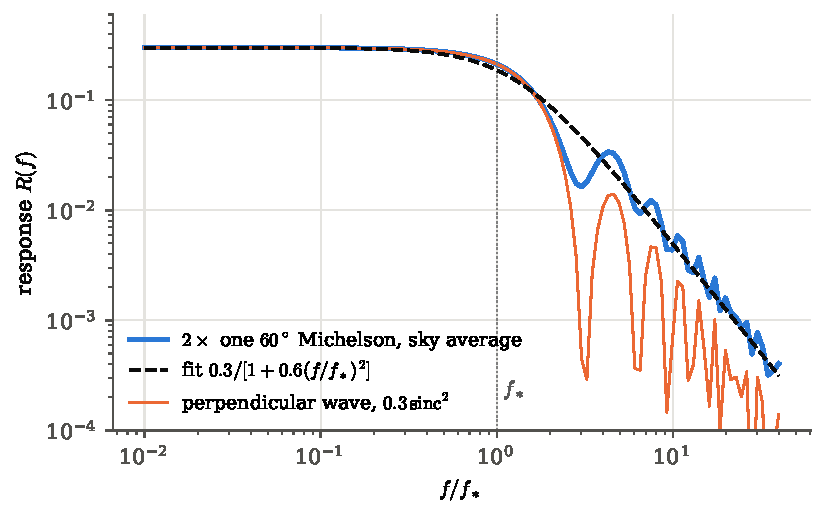
\includegraphics[width=0.8\linewidth]{figures/chT2/lisa_response.pdf}
\caption{The sky- and polarisation-averaged response of LISA against frequency in units of $f_*=c/(2\pi L)$. Blue: computed from the light-travel integrals \eqref{T2g:eq:leg} for one $60^\circ$ Michelson channel and doubled for two channels. Dashed: the fit of Robson et al. Orange: a wave arriving perpendicular to the arms, whose response $\mathrm{sinc}^2(f/f_*)$ vanishes whenever a whole number of cycles fits into the round trip. Averaging over directions fills in those zeros, but the $f^{-2}$ fall above $f_*$ remains.}
\label{T2g:fig:response}
\end{figure}

\Cref{T2g:fig:response} shows the result. At low frequency it is $\TwRzero$, the $\tfrac3{10}$ found above. At $f_*$ it has dropped to $\TwRstarRatio$ of that (the fit $R(f)=\tfrac3{10}/[1+0.6(f/f_*)^2]$ of \cite[eq.~(9)]{Robson2019} gives $0.625$), and well above $f_*$ it falls as $f^{\TwRslope}$, the $f^{-2}$ of the single-arm argument. Between about $2f_*$ and $10f_*$ our single-Michelson response wiggles around the fit by up to $\TwRfitDev\%$: these are the zeros of the individual arm responses, partly filled in by the sky average. The fit smooths them over, and the full response used in research analyses adds the third, high-frequency channel of the triangle \cite{Robson2019}.

\begin{keyidea}[The numbers that turn a source into an average source]
A detector reports $h=F_+h_++F_\times h_\times$. Averaged over the sky and the polarisation angle, a right-angle interferometer has $\langle F_+^2\rangle=\langle F_\times^2\rangle=\tfrac15$; a $60^\circ$ channel has $\tfrac34$ of that, $\tfrac3{20}$, and LISA's two channels together $\tfrac3{10}$. Averaging a circular binary over its inclination multiplies the signal power by $\tfrac45$. Above the transfer frequency $f_*=c/(2\pi L)$ the wave changes while the light is in flight and the response falls as $f^{-2}$.
\end{keyidea}

\paragraph{What the sky average leaves out.}
LISA orbits the Sun, so a source's signal is Doppler shifted back and forth over a year, and the triangle rotates, so the antenna patterns \eqref{T2g:eq:Fplus} change slowly with time \cite[eqs.~(16)--(17)]{BarackCutler2004}. The phase is modulated by $2\pi fR\sin\theta_S\cos(2\pi t/{\rm yr}-\phi_S)$, with $R=1\,{\rm AU}/c=499$\,s and $(\theta_S,\phi_S)$ the source's sky position \cite[eq.~(33)]{BarackCutler2004}. At $f=10$\,mHz the amplitude of this modulation is $2\pi\times0.01\times499\approx31$\,rad, so it is easily measured, and it is how LISA locates sources on the sky. The sky-averaged response drops that information and replaces the real, moving detector by an average one. For forecasts of an environment, which acts on the phase evolution and not on the sky position, the averaged response is adequate, and the signal-to-noise ratios it gives are good to a factor of about two \cite{Robson2019}.

\paragraph{Where this is used.}
The response rule \eqref{T2g:eq:response} is what turns a template into the predicted data stream in the detection problem of \cref{10b:sec:detection}. The averages $\tfrac45$ and $\tfrac3{10}$ are the ones built into the sky-averaged waveform and the sensitivity curve of \cref{T2a:sec:lisa}, which \cref{10b:sec:robson} checks against its source; $f_*$ and the high-frequency fall of the response set the shape of that curve above about $20$\,mHz.
\section{Why a compact binary chirps}
\label{T2a:sec:chirp}

Take two black holes, masses $m_1$ and $m_2$, on a circular orbit of radius $r$. \Cref{T2g:sec:quadrupole} showed that the pair radiates gravitational waves at twice its orbital frequency, with the power $P_{\rm GW}=\tfrac{32}{5}(G/c^5)\mu^2r^4\omega^6$ of \eqref{T2g:eq:power-binary}, and the energy flux of \cref{T2g:sec:energy} says that this power is real energy leaving the system. The pair therefore has less and less orbital energy, so it must sit deeper in its own potential well, on a smaller orbit. A smaller orbit is a faster orbit, and since $P_{\rm GW}\propto r^4\omega^6\propto r^{-5}$, a faster orbit radiates far more strongly. The process runs away: the orbit shrinks ever faster, and the frequency of the wave rises ever faster until the holes merge. Played as sound, the signal is a rising whistle, a \newterm{chirp}.

Every statistics calculation with such a signal starts from one question: \emph{given the two masses and the frequency $f$ of the wave we see today, how fast is $f$ rising, and how long is left before the merger?} The answer is a single formula for $\dot f$. The time to merger, the number of cycles, the phase of the wave and the end of the inspiral all follow from it.

\subsection{The inputs}

As with the Poisson process of \cref{ch:02}, we first separate what goes in from what comes out. Four things go in, and only the first two are new.
\begin{enumerate}[itemsep=1pt]
  \item \emph{Physical: Newtonian circular orbits.} The two bodies obey Newton's gravity and move on a circle. The two-body problem reduces, as usual, to one body of reduced mass $\mu=m_1m_2/M$ circling a fixed mass $M=m_1+m_2$, with Kepler's third law $\omega^2=GM/r^3$ for the orbital angular frequency $\omega$.
  \item \emph{Physical: slow evolution.} One orbit takes much less time than the orbit takes to shrink noticeably. So at each moment the orbit is a circle of the current radius, and the orbital energy simply drains into the waves, $\dd E/\dd t=-P_{\rm GW}$. We check this with numbers at the end of the section.
  \item \emph{Derived earlier: the radiated power} $P_{\rm GW}=\tfrac{32}{5}(G/c^5)\mu^2r^4\omega^6$ of \eqref{T2g:eq:power-binary}, which came from the linearised field equation and the energy flux in \cref{T2g:sec:quadrupole}, and the wave frequency $f=\omega/\pi$ of \eqref{T2g:eq:twice}.
  \item \emph{Mathematical:} $r(t)$ is smooth, so we may differentiate it.
\end{enumerate}
That only one combination of the masses matters is \emph{not} an input; it comes out of the derivation.

\subsection{From the radiated power to the chirp}

\paragraph{Energy and power as functions of the wave frequency.}
The frequency is what the detector measures, so we trade $r$ for $f$ using Kepler, $r=(GM/\omega^2)^{1/3}$ with $\omega=\pi f$:
\begin{align}
  E&\eqby{1}-\frac{GM\mu}{2r}\eqby{2}-\frac{\mu}{2}\,(\pi GMf)^{2/3},\label{T2a:eq:Ef}\\
  P_{\rm GW}&\eqby{3}\frac{32}{5}\frac{G}{c^5}\,\mu^2(GM)^{4/3}(\pi f)^{10/3}
  \eqby{4}\frac{32}{5}\frac{c^5}{G}\Big(\frac{\pi G\mathcal M f}{c^3}\Big)^{10/3},
  \qquad \mathcal M\equiv\mu^{3/5}M^{2/5}=\frac{(m_1m_2)^{3/5}}{(m_1+m_2)^{1/5}} .\label{T2a:eq:Pf}
\end{align}
\begin{explain}
  \item Kinetic plus potential energy of a circular orbit: $\tfrac12\mu v^2-GM\mu/r$ with $v^2=GM/r$.
  \item $1/r=(\omega^2/GM)^{1/3}$, so $GM/r=(GM)^{2/3}\omega^{2/3}$.
  \item $r^4\omega^6=(GM)^{4/3}\omega^{-8/3}\omega^6=(GM)^{4/3}\omega^{10/3}$.
  \item Collect the masses: $\mu^2M^{4/3}=(\mu^{3/5}M^{2/5})^{10/3}$, and the powers of $G$ and $c$ rearrange as $G^{7/3}/c^5=(c^5/G)(G/c^3)^{10/3}$.
\end{explain}
The combination $\mathcal M$ is the chirp mass of \eqref{T2g:eq:amp}: it appeared there in the amplitude of the wave and appears here again, on its own, in step (4).

\paragraph{The chirp rate.}
Energy balance says $\dd E/\dd t=-P_{\rm GW}$. Since $E$ depends on time only through $f$, $\dd E/\dd t=(\dd E/\dd f)\,\dot f$, so
\begin{align}
  \dot f&\eqby{1}\frac{P_{\rm GW}}{\lvert\dd E/\dd f\rvert}
  \eqby{2}\frac{\tfrac{32}{5}\tfrac{G^{7/3}}{c^5}\mu^2M^{4/3}(\pi f)^{10/3}}{\tfrac{\mu}{3}(\pi GM)^{2/3}f^{-1/3}}
  \eqby{3}\frac{96}{5}\,\pi^{8/3}\Big(\frac{G\mathcal M}{c^3}\Big)^{5/3}f^{11/3}.\label{T2a:eq:fdot}
\end{align}
\begin{explain}
  \item Energy balance, with $\dd E/\dd f<0$ (a higher frequency is a more bound orbit).
  \item $P_{\rm GW}$ from step (3) of \eqref{T2a:eq:Pf}; $\dd E/\dd f=-\tfrac{\mu}{3}(\pi GM)^{2/3}f^{-1/3}$ from \eqref{T2a:eq:Ef}.
  \item One $\mu$ cancels; $\mu M^{4/3}/M^{2/3}=\mu M^{2/3}=\mathcal M^{5/3}$, $G^{7/3}/G^{2/3}=G^{5/3}$ so $G^{5/3}/c^5=(G/c^3)^{5/3}$, and $\pi^{10/3}/\pi^{2/3}\cdot f^{10/3}f^{1/3}=\pi^{8/3}f^{11/3}$.
\end{explain}

\begin{keyidea}[The Newtonian chirp]
A circular binary radiating quadrupole waves sweeps up in frequency at the rate
$\dot f=\frac{96}{5}\pi^{8/3}(G\mathcal M/c^3)^{5/3}f^{11/3}$. At this order the masses enter only through the chirp mass $\mathcal M=(m_1m_2)^{3/5}/(m_1+m_2)^{1/5}$, so the data measure $\mathcal M$ first and the separate masses only through smaller corrections.
\end{keyidea}

The product $G\mathcal M/c^3$ has units of time. For the Sun it is $GM_\odot/c^3=4.93\,\mu$s, which is the handiest number in gravitational-wave astronomy: a mass in solar units times $4.93\,\mu$s is that mass as a time.

\paragraph{Frequency against time, and the number of cycles.}
Since $\dd t=\dd f/\dot f$, the time left before the frequency runs off to infinity (the formal coalescence time $t_c$) is
\begin{align}
  \tau(f)\equiv t_c-t
  &\eqby{1}\int_f^\infty\frac{\dd f'}{\dot f(f')}
  \eqby{2}\frac{5}{96}\pi^{-8/3}\Big(\frac{G\mathcal M}{c^3}\Big)^{-5/3}\cdot\frac38 f^{-8/3}
  =\frac{5}{256}\Big(\frac{G\mathcal M}{c^3}\Big)^{-5/3}(\pi f)^{-8/3},\label{T2a:eq:tau}
\end{align}
\begin{explain}
  \item Time is the integral of $\dd f/\dot f$ along the sweep.
  \item $\int_f^\infty f'^{-11/3}\dd f'=\tfrac38 f^{-8/3}$; then $\tfrac{5}{96}\cdot\tfrac38=\tfrac{5}{256}$ and $\pi^{-8/3}f^{-8/3}=(\pi f)^{-8/3}$.
\end{explain}
and inverting, $f(\tau)=\frac{1}{8\pi}\big(G\mathcal M/c^3\big)^{-5/8}\big(5/\tau\big)^{3/8}$ \cite[eq.~(24)]{Robson2019}. The number of wave cycles between $f_1$ and $f_2$ is $N=\int f\,\dd t=\int f\,\dd f/\dot f$:
\begin{equation}
  N(f_1,f_2)=\frac{1}{32\pi^{8/3}}\Big(\frac{G\mathcal M}{c^3}\Big)^{-5/3}\big(f_1^{-5/3}-f_2^{-5/3}\big),
  \label{T2a:eq:Ncyc}
\end{equation}
from $\int f^{-8/3}\dd f=-\tfrac35f^{-5/3}$ and $\tfrac35\cdot\tfrac{5}{96}=\tfrac1{32}$. The low-frequency end dominates: most cycles are spent where the binary is slow.

\paragraph{Where the inspiral ends.}
In Newton's theory circular orbits exist all the way down. In general relativity they stop being stable inside the \newterm{innermost stable circular orbit} (ISCO), $r_{\rm ISCO}=6GM/c^2$, three Schwarzschild radii; inside it the small body plunges. Kepler's law there gives $\omega^2=c^6/(216\,G^2M^2)$, so
\begin{equation}
  f_{\rm ISCO}=\frac{c^3}{6^{3/2}\pi GM}\approx 4.4\,\mathrm{kHz}\times\frac{M_\odot}{M}.
  \label{T2a:eq:fisco}
\end{equation}
Papers on dark-matter environments stop their inspirals here \cite{Eda2015,Kim2023}, and so do we.

\begin{figure}[htbp]
\centering
\begin{tikzpicture}[scale=1.0]
  \draw[formblue,thick,domain=0:18.4,samples=600,smooth,variable=\t]
    plot ({2.4*((18.85-\t)/18.85)^(0.4)*cos(\t r)},{2.4*((18.85-\t)/18.85)^(0.4)*sin(\t r)});
  \fill[black] (0,0) circle (2.2pt);
  \fill[fibreorange] (2.4,0) circle (1.6pt);
  \node[lbl,anchor=west] at (2.5,0) {$m_2$ (start)};
  \foreach \R in {3.0,3.4,3.8}{\draw[faint] (15:\R) arc (15:45:\R);}
  \node[lbl,align=left,anchor=west] at (1.2,3.4) {energy carried\\ off by waves};
  \begin{scope}[xshift=5.4cm,yshift=-1.6cm]
    \draw[->] (0,0) -- (5.6,0);
    \node[lbl,below] at (2.5,0) {time $t$};
    \draw[->] (0,0) -- (0,3.4) node[left,lbl] {$f$};
    \draw[formblue,thick,domain=0:4.95,samples=200,smooth] plot (\x,{0.45*((5-0)/(5-\x))^(0.375)});
    \draw[faint,dashed] (5,0) -- (5,3.3);
    \node[lbl,below] at (5,0) {$t_c$};
    \node[lbl,anchor=west,align=left] at (0.3,2.6) {$f\propto (t_c-t)^{-3/8}$};
  \end{scope}
\end{tikzpicture}
\caption{The chirp. Left: the light body's path around the heavy one (dot) for a Newtonian inspiral, the last three turns, drawn to scale in shape ($r\propto(\phi_c-\phi)^{2/5}$, which follows from $r\propto\tau^{1/4}$ and $\phi\propto\tau^{5/8}$); each turn is tighter and quicker than the last. Right: the wave frequency of \eqref{T2a:eq:tau} inverted, rising slowly for a long time and then very fast just before $t_c$.}
\label{T2a:fig:chirp-cartoon}
\end{figure}

\subsection{The phase of the wave, and the two numbers that fix it}
\label{T2g:sec:tc-phic}

The detector does not record the frequency; it records the wave, $h(t)=A(t)\cos\phi(t)$ for one polarisation, with the amplitude $A\propto f^{2/3}$ of \eqref{T2g:eq:amp} and a phase $\phi(t)$ whose rate of change is the angular frequency, $\dot\phi=2\pi f$. So the phase is the integral of the frequency history. Write $T_{\mathcal M}\equiv G\mathcal M/c^3$, the chirp mass as a time, and $\tau=t_c-t$. The inverse of \eqref{T2a:eq:tau} is $2\pi f(\tau)=\tfrac14T_{\mathcal M}^{-5/8}5^{3/8}\tau^{-3/8}$, and since $\dd\tau=-\dd t$,
\begin{align}
  \phi(t)
  &\eqby{1}\phi_c-\int_0^{\tau}2\pi f(\tau')\,\dd\tau'
  \eqby{2}\phi_c-\tfrac14T_{\mathcal M}^{-5/8}5^{3/8}\cdot\tfrac85\,\tau^{5/8}
  \eqby{3}\phi_c-2\Big(\frac{\tau}{5T_{\mathcal M}}\Big)^{5/8},
  \label{T2g:eq:phit}
\end{align}
\begin{explain}
  \item The phase grows by $2\pi f\,\dd t$ in each moment. Integrating backwards from the end, where it reaches the value $\phi_c$, the phase at time $t$ is $\phi_c$ minus everything still to come.
  \item $\int_0^\tau\tau'^{-3/8}\dd\tau'=\tfrac85\tau^{5/8}$.
  \item $\tfrac14\cdot\tfrac85\cdot5^{3/8}=\tfrac25\cdot5^{3/8}=2\cdot5^{-5/8}$, and $5^{-5/8}T_{\mathcal M}^{-5/8}\tau^{5/8}=(\tau/5T_{\mathcal M})^{5/8}$.
\end{explain}
which is \cite[eq.~(17)]{CutlerFlanagan1994}. Two integration constants appeared on the way, and both are now parameters of the signal.

\emph{The time of coalescence $t_c$} is the moment at which the Newtonian frequency \eqref{T2a:eq:tau} would formally run off to infinity. The real inspiral ends a little earlier, at the ISCO, but $t_c$ is a convenient label for ``when it all happens''. Changing $t_c$ by $\Delta$ slides the whole signal along the time axis, $h(t)\to h(t-\Delta)$, without changing its shape.

\emph{The phase at coalescence $\phi_c$} is the value of the phase at $t_c$. Since the wave phase is twice the orbital phase, changing $\phi_c$ by $\delta$ is the same as having started the two bodies at a different place on their orbit, turned by $\delta/2$ about the orbital axis. It does not change $t_c$, the masses or the frequency history; it only shifts the crests of the wave.

\emph{Why they are nuisance parameters.} Neither number says anything about the physics of the source. $t_c$ records when, on our clocks, the binary happened to merge; $\phi_c$ records where the two bodies happened to be on their orbit at that moment. Both are pure accident, both are unknown before the data arrive, and both must nevertheless be in the template: a template whose crests sit half a cycle away from the signal's crests correlates with it negatively, however right its masses. In the language of \cref{ch:05} they are \newterm{nuisance parameters}, unknowns we must fit or integrate over but do not care about. \Cref{10b:sec:phase-time} shows that both can be searched over almost for free, the phase with two filters and the arrival time with one Fourier transform, and \cref{T2a:sec:spa} shows why: in the frequency domain they enter the phase only as the straight line $2\pi ft_c-\phi_c$.

\subsection{Examples: the benchmark binaries of the book}

Two systems recur in the dark-matter literature and in \cref{ch:10}. In both, a light black hole falls into a much heavier one. Binaries are named by their mass ratio $q=m_2/m_1$: comparable-mass binaries have $q\sim1$, \newterm{intermediate mass-ratio inspirals} (IMRIs) roughly $q\sim10^{-2}$--$10^{-4}$, and \newterm{extreme mass-ratio inspirals} (EMRIs) $q\lesssim10^{-4}$; the boundary is a convention, and papers place it differently \cite{Speeney2022,Kim2023}. A small $q$ is what makes these systems good probes. By \eqref{T2a:eq:fdot}, $\dot f\propto\mathcal M^{5/3}\approx m_2\,m_1^{2/3}$ when $m_2\ll m_1$, so a light companion spirals in slowly and completes a huge number of orbits inside the environment.

\paragraph{The numbers.}
Every number quoted in the examples below comes from a few lines of \pyname{01_chirp.py}, which apply \eqref{T2a:eq:fisco}, \eqref{T2a:eq:tau}, \eqref{T2a:eq:Ncyc} and \eqref{T2a:eq:fdot} to a pair of masses:

\pyfile[firstline=28,lastline=33,firstnumber=28]{code/chT2/01_chirp.py}{From two masses to the end of the inspiral}

\noindent Line 29 is the ISCO frequency. Line 30 is the time left at that frequency, \eqref{T2a:eq:tau}. Line 31 adds four years to that time and inverts, giving the frequency four years before the ISCO. Line 32 counts the cycles between the two frequencies, and line 33 is the slow-evolution number checked in the last example. The helper functions (\pyname{tau_of_f}, \pyname{cycles}, and so on) sit in \pyname{lib_lisa.py} and are one-line transcriptions of the equations above.

\paragraph{Example: the EMRI of Kim et al.}
A $1\,M_\odot$ black hole falls into a $10^4\,M_\odot$ one \cite[Sec.~III F]{Kim2023}. Kim et al.\ call it an IMRI; with $q=10^{-4}$ it sits on the boundary, and we call it the EMRI. The chirp mass is
\[
  \mathcal M=\frac{(10^4\cdot1)^{3/5}}{(10^4+1)^{1/5}}\approx\frac{10^{2.4}}{10^{0.8}}=10^{1.6}\approx 40\,M_\odot,
\]
and the code gives $\mathcal M=\TwEmriMc\,M_\odot$. By \eqref{T2a:eq:fisco} the inspiral ends at $f_{\rm ISCO}=4.4\,\mathrm{kHz}/10^4\approx\TwEmrifisco$\,Hz, inside the LISA band ($10^{-4}$--$1$\,Hz). Four years earlier, from \eqref{T2a:eq:tau}, the frequency was $\TwEmriffouryr$\,mHz, and by \eqref{T2a:eq:Ncyc} the binary completes $N=\TwEmriNcyc$ wave cycles in those four years.

\paragraph{Example: the IMRI of Eda et al.\ and Coogan et al.}
A $1.4\,M_\odot$ object falls into a $10^3\,M_\odot$ black hole \cite{Eda2015,Coogan2022}. Now $\mathcal M=\TwImriMc\,M_\odot$ and $f_{\rm ISCO}=\TwImrifisco$\,Hz, above LISA's band: the last stretch of this inspiral is invisible to LISA. Four years before the ISCO the frequency is $\TwImriffouryr$\,mHz, and $N=\TwImriNcyc$ cycles follow. \Cref{T2a:fig:chirp-tracks} shows both frequency tracks.

\begin{figure}[htbp]
\centering
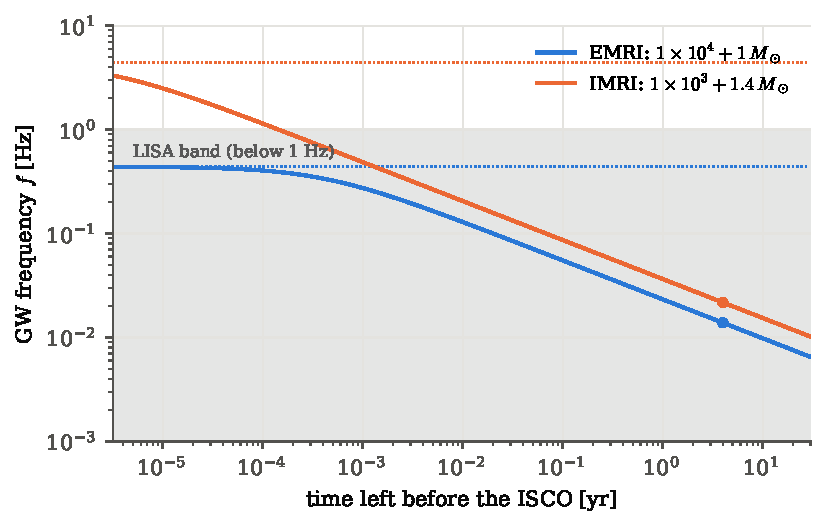
\includegraphics[width=0.82\linewidth]{figures/chT2/chirp_tracks.pdf}
\caption{Frequency against the time left before the ISCO for the two benchmark binaries. Far from the end both tracks are straight lines of slope $-3/8$ on these log axes; close to the end they flatten onto $f_{\rm ISCO}$ (dotted). Dots mark the frequency four years before the ISCO. The shaded band is LISA's frequency range: the IMRI leaves it before its ISCO, the EMRI does not.}
\label{T2a:fig:chirp-tracks}
\end{figure}

\paragraph{Example: a GW150914-like binary passing through the LISA band.}
Robson, Cornish and Liu note that a binary like the first LIGO detection, five years before merger, sweeps from $16$ to $29$\,mHz during a four-year mission \cite[Sec.~2]{Robson2019}. We can check this with \eqref{T2a:eq:tau}. Take $m_1=36$, $m_2=29\,M_\odot$, so $\mathcal M=\TwGWMc\,M_\odot$ and $G\mathcal M/c^3=28.1\times4.93\,\mu{\rm s}=1.38\times10^{-4}$\,s. Five years before merger, $\tau=1.58\times10^8$\,s, and
\begin{align*}
  f&\eqby{1}\frac{1}{8\pi\,G\mathcal M/c^3}\Big(\frac{5\,G\mathcal M/c^3}{\tau}\Big)^{3/8}
  \eqby{2}\frac{1}{3.47\times10^{-3}\,{\rm s}}\big(4.37\times10^{-12}\big)^{3/8}\\
  &\eqby{3}288\,{\rm Hz}\times5.5\times10^{-5}\approx16\,{\rm mHz}.
\end{align*}
\begin{explain}
  \item The inverse of \eqref{T2a:eq:tau}.
  \item $8\pi\times1.38\times10^{-4}=3.47\times10^{-3}$ and $5\times1.38\times10^{-4}/1.58\times10^8=4.37\times10^{-12}$.
  \item $(4.37\times10^{-12})^{3/8}=10^{-11.36\times3/8}=10^{-4.26}$.
\end{explain}
The same steps with $\tau=1$\,yr give $29$\,mHz. The code returns $\TwGWfFive$ and $\TwGWfOne$\,mHz, and the binary completes $\TwGWNcyc$ cycles in between.

\paragraph{Example: checking the slow-evolution input.}
Input 2 assumed the orbit barely changes during one cycle. The fractional change of $f$ during one cycle (duration $1/f$) is $\dot f/f^2=\frac{96}{5}\pi^{8/3}(G\mathcal Mf/c^3)^{5/3}$, largest at the ISCO. The code gives $\TwEmriadiab$ for the EMRI and $\TwImriadiab$ for the IMRI. Even on the last orbit the frequency changes by less than a part in a thousand per cycle, so treating the orbit as a slowly shrinking circle is safe \cite[eq.~(25)]{CutlerFlanagan1994}.

\paragraph{What a million cycles buys.}
A template that drifts out of step with the signal by a single cycle, out of millions, no longer matches it. So the data pin down whatever sets the number of cycles very precisely \cite[Sec.~I]{CutlerFlanagan1994}. By \eqref{T2a:eq:Ncyc}, $N\propto\mathcal M^{-5/3}$, so a fractional change $\delta\mathcal M/\mathcal M$ shifts the count by $\delta N=\frac53N\,\delta\mathcal M/\mathcal M$. Requiring $\delta N\lesssim1$ gives $\delta\mathcal M/\mathcal M\lesssim3/(5N)$, of order $10^{-7}$ for the EMRI. This is only a rough estimate: noise, a finite signal-to-noise ratio and correlations with other parameters weaken it, and the Fisher matrix of \cref{ch:10} does the calculation properly. For this EMRI with five years of data and signal-to-noise ratio $15$, Kim et al.\ find $\mathcal M=39.8^{+0.0012}_{-0.0006}\,M_\odot$ (95\% range), a fractional error of about $2\times10^{-5}$ \cite[Fig.~4]{Kim2023}. The parameters that only set the amplitude, such as the distance, are measured with fractional errors of order one over the signal-to-noise ratio. This difference is the reason an environment is detectable at all: it acts on the phase, the most precisely measured part of the signal.

\begin{pitfall}[Which mass is measured]
The wave reaches us stretched by the cosmological redshift $z$, and a stretched chirp from mass $\mathcal M$ is indistinguishable from an unstretched chirp from mass $(1+z)\mathcal M$. The data measure the \emph{detector-frame} (redshifted) chirp mass $(1+z)\mathcal M$, and \eqref{T2a:eq:fdot}--\eqref{T2a:eq:fisco} must be used with it \cite[Sec.~2]{Robson2019}. For the nearby benchmark binaries $z\ll1$ and the difference is negligible.
\end{pitfall}

\paragraph{Where this is used.}
The chirp rate \eqref{T2a:eq:fdot} and the binding energy \eqref{T2a:eq:Ef} are the vacuum baseline that \cref{10b:sec:env-derive} perturbs when an environment drains extra energy; the frequency four years before the ISCO and the cycle counts fix the band and the benchmark source of \cref{10b:sec:benchmark}; and $t_c$, $\phi_c$ are the two nuisance parameters that \cref{10b:sec:phase-time} maximises over and that the Fisher matrix of \cref{10b:sec:fisher} carries alongside the masses.
\section{The chirp in the frequency domain}
\label{T2a:sec:spa}

The detector records a time series, but the likelihood of \cref{10b:sec:noise-fd} is written in the frequency domain. There the stationary noise of the detector is simple: different Fourier components are independent, each with a variance set by the noise spectrum $S_n(f)$, and the log-likelihood is $-\tfrac12(d-h\,|\,d-h)$ with the noise-weighted inner product $(a\,|\,b)=4\,\mathrm{Re}\int_0^\infty\tilde a\tilde b^*/S_n\,\dd f$. So the statistics needs the Fourier transform of the chirp of \cref{T2a:sec:chirp}, as a formula in which the masses, the arrival time $t_c$ and the phase $\phi_c$ appear explicitly.

A chirp makes this easy. At each moment it has one frequency, and it passes through each frequency once. So we ask in words: \emph{which part of the time series builds the Fourier component at frequency $f$?} The answer is: essentially only the stretch during which the chirp's own frequency is close to $f$. At all other times the chirp and the probe wave $e^{-2\pi ift}$ run at different rates, their product oscillates, and the oscillations cancel in the integral. Only near the moment $t_f$ at which the chirp's frequency equals $f$ do the two stay in step long enough to add up. Turning this sentence into a formula is the \newterm{stationary-phase approximation} (SPA) \cite[eq.~(21)]{CutlerFlanagan1994}.

\subsection{The Fourier convention, and why only positive frequencies count}

The book's convention, used in every chapter, is
\begin{equation}
  \tilde h(f)=\int_{-\infty}^{\infty}h(t)\,e^{-2\pi ift}\,\dd t,\qquad
  h(t)=\int_{-\infty}^{\infty}\tilde h(f)\,e^{2\pi ift}\,\dd f ,
  \label{T2g:eq:fourier}
\end{equation}
with $f$ in cycles per second, so that no factors of $2\pi$ stand in front of the integrals. A detector output is a real number at every instant, and that fixes the negative frequencies in terms of the positive ones:
\begin{equation}
  \tilde h(-f)\eqby{1}\int h(t)\,e^{+2\pi ift}\,\dd t\eqby{2}\Big[\int h(t)\,e^{-2\pi ift}\,\dd t\Big]^*\eqby{3}\tilde h(f)^* .
  \label{T2g:eq:reality}
\end{equation}
\begin{explain}
  \item The definition at $-f$.
  \item $h(t)$ is real, so complex-conjugating the integrand only flips the sign in the exponent.
  \item The definition at $+f$.
\end{explain}
For example, the tone $\cos2\pi f_0t=\tfrac12e^{2\pi if_0t}+\tfrac12e^{-2\pi if_0t}$ has $\tilde h(f)=\tfrac12\delta(f-f_0)+\tfrac12\delta(f+f_0)$: half its weight sits at $+f_0$ and half, the complex conjugate, at $-f_0$. Since the negative half carries no new information, every quantity built from a real signal can be written with $f>0$ only, at the price of a factor two. That is where the $4$ in the inner product comes from: the $2$ of the one-sided noise spectrum of \cref{10b:sec:noise-fd} times the $2$ from folding $-f$ onto $+f$. So it is enough to know $\tilde h(f)$ for $f>0$.

\begin{figure}[htbp]
\centering
\begin{tikzpicture}
\begin{axis}[width=11cm,height=4.2cm,axis x line=middle,axis y line=none,xmin=-4.2,xmax=4.4,ymin=-1.35,ymax=1.5,
  xtick=\empty,ytick=\empty,xlabel={$t$},xlabel style={anchor=west},
  clip=false]
  \fill[formblue!10] (axis cs:-0.58,-1.25) rectangle (axis cs:0.58,1.25);
  \addplot[formblue,thick,domain=-4:4,samples=900] {cos(deg(3*x^2))};
  \draw[faint] (axis cs:0,-0.08) -- (axis cs:0,0.08);
  \node[lbl,anchor=north] at (axis cs:0,-0.1) {$t_f$};
  \node[lbl,anchor=south] at (axis cs:0,1.25) {in step: adds up};
  \node[lbl,anchor=south] at (axis cs:-2.9,1.1) {out of step: cancels};
  \node[lbl,anchor=south] at (axis cs:2.9,1.1) {out of step: cancels};
\end{axis}
\end{tikzpicture}
\caption{The real part of the integrand $e^{i[\phi(t)-2\pi ft]}$ near the moment $t_f$ at which the chirp has frequency $f$, for a chirp whose frequency rises linearly: the phase difference grows like $(t-t_f)^2$. In the shaded window, of width about $1/\sqrt{\dot f}$, the integrand barely turns and its contributions add. Outside, positive and negative lobes alternate faster and faster and cancel.}
\label{T2a:fig:spa-picture}
\end{figure}

\subsection{The stationary-phase formula}

\emph{Inputs.} The signal is $h(t)=A(t)\cos\phi(t)$, with an amplitude that changes slowly compared with the phase ($\dot A/A\ll\dot\phi$) and a frequency $\dot\phi/2\pi$ that changes slowly, $\ddot\phi\ll\dot\phi^2$. The second condition is $\dot f/f^2\ll1$, the slow-evolution number already checked in \cref{T2a:sec:chirp}. We want $\tilde h(f)$ for $f>0$.

\emph{Two exponentials.} Writing the cosine as $\cos\phi=\tfrac12(e^{i\phi}+e^{-i\phi})$,
\begin{equation}
  \tilde h(f)=\frac12\int A(t)\,e^{i[\phi(t)-2\pi ft]}\,\dd t+\frac12\int A(t)\,e^{-i[\phi(t)+2\pi ft]}\,\dd t .
  \label{T2g:eq:two-exp}
\end{equation}
\emph{The second integral is negligible.} Its phase $\phi(t)+2\pi ft$ always grows, at the rate $\dot\phi+2\pi f\ge2\pi f$, so its integrand turns steadily and its positive and negative lobes cancel. Integrating by parts once shows how well: $\int Ae^{i\theta}\dd t=[Ae^{i\theta}/(i\dot\theta)]-\int(\dd/\dd t)(A/i\dot\theta)\,e^{i\theta}\dd t$, so the integral is of order $A/(2\pi f)$, the amplitude times the time the integrand needs to turn once. We will see that the first integral is of order $A/\sqrt{\dot f}$; the ratio is $\sqrt{\dot f}/f=(\dot f/f^2)^{1/2}\ll1$.

\emph{Where the first integral comes from.} Call its phase $\vartheta(t)\equiv\phi(t)-2\pi ft$. It is \emph{stationary}, $\dot\vartheta=0$, where $\dot\phi=2\pi f$: at the moment $t_f$ when the chirp's own frequency equals $f$. Near that moment Taylor-expand, $\vartheta(t)=\vartheta(t_f)+0\cdot(t-t_f)+\tfrac12\ddot\phi(t_f)(t-t_f)^2+\dots$, the linear term vanishing by the definition of $t_f$, and freeze the slowly varying amplitude at $A(t_f)$. Then
\begin{align}
  \tilde h(f)
  &\eqby{1}\frac12A(t_f)\,e^{i\vartheta(t_f)}\int_{-\infty}^{\infty}e^{\frac i2\ddot\phi(t_f)\,s^2}\,\dd s
  \eqby{2}\frac12A(t_f)\,e^{i\vartheta(t_f)}\sqrt{\frac{2\pi}{\ddot\phi(t_f)}}\;e^{i\pi/4}\nonumber\\
  &\eqby{3}\frac12A(t_f)\,\dot f(t_f)^{-1/2}\,e^{-i\Psi(f)},\qquad
  \Psi(f)\equiv2\pi ft_f-\phi(t_f)-\frac\pi4 .\label{T2a:eq:spa}
\end{align}
\begin{explain}
  \item The expansion with $s=t-t_f$. The limits can be taken to $\pm\infty$, because far from $t_f$ the integrand oscillates ever faster and contributes nothing more (\cref{T2a:fig:spa-picture}).
  \item The Fresnel integral, derived just below: $\int e^{ias^2/2}\dd s=\sqrt{2\pi/a}\,e^{i\pi/4}$ for $a>0$, here with $a=\ddot\phi(t_f)>0$ because the frequency rises.
  \item $\ddot\phi=2\pi\dot f$, so $\sqrt{2\pi/\ddot\phi}=\dot f^{-1/2}$. Collecting the phases, $\vartheta(t_f)+\tfrac\pi4=\phi(t_f)-2\pi ft_f+\tfrac\pi4=-\Psi(f)$.
\end{explain}

\emph{The Fresnel integral.} The integrand $e^{ias^2/2}$ has modulus one everywhere, so the integral converges only because of the cancellations. Make that explicit by adding a small damping $e^{-\epsilon s^2}$, $\epsilon>0$, and letting $\epsilon\to0$ at the end. With $b\equiv\epsilon-ia/2$,
\begin{align}
  \int_{-\infty}^\infty e^{-\epsilon s^2+ias^2/2}\,\dd s
  &\eqby{1}\int_{-\infty}^\infty e^{-bs^2}\,\dd s
  \eqby{2}\sqrt{\frac\pi b}
  \;\xrightarrow{\ \epsilon\to0\ }\;
  \sqrt{\frac{\pi}{-ia/2}}
  \eqby{3}\sqrt{\frac{2\pi}{a}}\;e^{i\pi/4} .
  \label{T2g:eq:fresnel}
\end{align}
\begin{explain}
  \item Definition of $b$; its real part $\epsilon$ is positive, so the integral converges absolutely.
  \item The Gaussian integral $\int e^{-bs^2}\dd s=\sqrt{\pi/b}$, familiar for real $b>0$. Both sides are analytic functions of $b$ in the half-plane $\mathrm{Re}\,b>0$ (with the square root positive for real $b$), and two analytic functions that agree on the positive real axis agree everywhere in that half-plane.
  \item $-i=e^{-i\pi/2}$, so $1/(-i)=e^{i\pi/2}$ and its square root is $e^{i\pi/4}$; the branch is the one that is continuous from $\mathrm{Re}\,b>0$, where $\arg b\to-\pi/2$ and $\arg\sqrt{1/b}\to+\pi/4$.
\end{explain}
The real and imaginary parts are the classic Fresnel integrals, $\int\cos(as^2/2)\dd s=\int\sin(as^2/2)\dd s=\sqrt{\pi/a}$; the phase $e^{i\pi/4}$ says they are equal.

\emph{How accurate is it?} The width of the window that contributes is set by the Gaussian factor in step (1): $\lvert t-t_f\rvert\lesssim1/\sqrt{\ddot\phi}\sim1/\sqrt{\dot f}$. During that window the chirp completes about $f/\sqrt{\dot f}=(\dot f/f^2)^{-1/2}$ cycles, which is large precisely when the slow-evolution number is small. The first neglected term of the Taylor expansion, $\tfrac16\dddot\phi\,(t-t_f)^3$, is of size $\dddot\phi/\ddot\phi^{3/2}$ across the window; with $\dddot\phi=2\pi\ddot f$ and $\ddot f=\tfrac{11}{3}\dot f^2/f$ for the Newtonian chirp, that is again of order $(\dot f/f^2)^{1/2}$. So the same condition makes the orbit adiabatic and the SPA accurate.\footnote{Cutler and Flanagan, Eda et al.\ and Kim et al.\ define the Fourier transform with $e^{+2\pi ift}$ and therefore write $e^{+i\Psi(f)}$. The function $\Psi(f)$ is the same; the two conventions give complex-conjugate $\tilde h$, and the inner product, the signal-to-noise ratio and the Fisher matrix, which contain only $\mathrm{Re}\,\tilde a\tilde b^*$, are unchanged.}

\paragraph{What the phase knows.}
Differentiate $\Psi$ and use $\dot\phi(t_f)=2\pi f$:
\begin{align}
  \frac{\dd\Psi}{\dd f}
  &\eqby{1}2\pi t_f+2\pi f\frac{\dd t_f}{\dd f}-\dot\phi(t_f)\frac{\dd t_f}{\dd f}
  \eqby{2}2\pi t(f),\qquad
  \frac{\dd^2\Psi}{\dd f^2}\eqby{3}\frac{2\pi}{\dot f}.\label{T2a:eq:psi-derivs}
\end{align}
\begin{explain}
  \item Product rule on $2\pi ft_f$ and chain rule on $\phi(t_f)$, since $t_f$ depends on $f$.
  \item The last two terms cancel because $\dot\phi(t_f)=2\pi f$. We write $t(f)\equiv t_f$.
  \item $\dd t/\dd f=1/\dot f$.
\end{explain}
In words: the slope of the Fourier phase is the time at which frequency $f$ arrives, and its curvature is $2\pi$ divided by the chirp rate. Whatever changes how fast the binary sweeps, an environment included, changes $\Psi$ through \eqref{T2a:eq:psi-derivs}. \Cref{T2a:sec:forces} applies exactly this equation to a binary that is losing energy to its surroundings as well as to waves.

\paragraph{The Newtonian waveform.}
Integrate \eqref{T2a:eq:psi-derivs} with $t(f)=t_c-\tau(f)$ from \eqref{T2a:eq:tau}:
\begin{align}
  \Psi(f)
  &\eqby{1}2\pi ft_c-2\pi\int\tau(f)\,\dd f+\text{const}
   \eqby{2}2\pi ft_c+2\pi\cdot\frac35\cdot\frac{5}{256}\Big(\frac{G\mathcal M}{c^3}\Big)^{-5/3}\pi^{-8/3}f^{-5/3}+\text{const}\nonumber\\
  &\eqby{3}2\pi ft_c-\phi_c-\frac\pi4+\frac{3}{128}\Big(\frac{\pi G\mathcal Mf}{c^3}\Big)^{-5/3}.\label{T2a:eq:psiN}
\end{align}
\begin{explain}
  \item Integrate $\dd\Psi/\dd f=2\pi t_c-2\pi\tau(f)$ once.
  \item $\tau=\tfrac{5}{256}(G\mathcal M/c^3)^{-5/3}\pi^{-8/3}f^{-8/3}$ and $\int f^{-8/3}\dd f=-\tfrac35f^{-5/3}$.
  \item $2\pi\cdot\tfrac{3}{256}\pi^{-8/3}=\tfrac{3}{128}\pi^{-5/3}$; the integration constant is named after the phase at coalescence, $-\phi_c-\pi/4$.
\end{explain}
This agrees with \cite[eq.~(24)]{CutlerFlanagan1994}, where the last term is written $\tfrac34(8\pi\mathcal Mf)^{-5/3}$ ($G=c=1$); $\tfrac34\cdot8^{-5/3}=\tfrac34\cdot\tfrac1{32}=\tfrac3{128}$. The phase constant $-\phi_c-\pi/4$ and the term $2\pi ft_c$ are exactly the two nuisance parameters of \cref{T2g:sec:tc-phic}, and in the frequency domain they enter only as a straight line in $f$: a shift of the arrival time is a phase that grows linearly with frequency.

\emph{The amplitude.} For the amplitude we need $A(t_f)$, the face-on amplitude of \eqref{T2g:eq:amp} at frequency $f$, with the distance now the luminosity distance $D_L$, and $\dot f$ from \eqref{T2a:eq:fdot}. With $T_{\mathcal M}=G\mathcal M/c^3$,
\begin{align}
  \tfrac12A\,\dot f^{-1/2}
  &\eqby{1}\frac12\cdot4T_{\mathcal M}^{5/3}(\pi f)^{2/3}\frac{c}{D_L}\cdot\Big(\frac{96}{5}\Big)^{-1/2}\pi^{-4/3}T_{\mathcal M}^{-5/6}f^{-11/6}
  \eqby{2}\sqrt{\frac{5}{24}}\;\pi^{-2/3}\,T_{\mathcal M}^{5/6}\,\frac{c}{D_L}\,f^{-7/6},
\end{align}
\begin{explain}
  \item $A=4(G\mathcal M)^{5/3}(\pi f)^{2/3}/(c^4D_L)=4T_{\mathcal M}^{5/3}(\pi f)^{2/3}c/D_L$, and $\dot f^{-1/2}=(\tfrac{96}5)^{-1/2}\pi^{-4/3}T_{\mathcal M}^{-5/6}f^{-11/6}$.
  \item $2(\tfrac{5}{96})^{1/2}=(\tfrac{20}{96})^{1/2}=(\tfrac5{24})^{1/2}$; $\pi^{2/3-4/3}=\pi^{-2/3}$; $T_{\mathcal M}^{5/3-5/6}=T_{\mathcal M}^{5/6}$; $f^{2/3-11/6}=f^{-7/6}$.
\end{explain}
so that
\begin{equation}
  \tilde h(f)=\mathcal A\,f^{-7/6}e^{-i\Psi(f)},\qquad
  \mathcal A=\sqrt{\frac{5}{24}}\;\pi^{-2/3}\Big(\frac{G\mathcal M}{c^3}\Big)^{5/6}\frac{c}{D_L},
  \label{T2a:eq:hf}
\end{equation}
the amplitude of Robson et al.\ \cite[eq.~(20)]{Robson2019} and of Kim et al.\ \cite[eq.~(45)]{Kim2023}, written out; the time-domain amplitude is that of Eda et al.\ \cite[eq.~(21)]{Eda2015}. A real source is not face-on, and the detector does not see both polarisations equally. By \eqref{T2g:eq:hpc} the polarisations of a circular binary have amplitudes $\tfrac12(1+x^2)$ and $x$ times $A$, with $x=\cos\iota$, and \cref{T2g:sec:detector} showed that averaging over the orientation of the orbit multiplies the signal power by $\tfrac45$, \eqref{T2g:eq:four-fifths}, while the average over sky position and polarisation is put into the noise curve (\cref{T2a:sec:lisa}). Hence the sky-averaged waveform $\tilde h=\sqrt{4/5}\,\mathcal A f^{-7/6}e^{-i\Psi}$ used in the forecasts \cite[eq.~(44)]{Kim2023}.

\begin{keyidea}[The signal model of the forecasts]
In the stationary-phase approximation a slowly chirping binary has $\tilde h(f)=\tfrac12A(t_f)\dot f^{-1/2}e^{-i\Psi(f)}$, with $\dd\Psi/\dd f=2\pi t(f)$ and $\dd^2\Psi/\dd f^2=2\pi/\dot f$. For the Newtonian chirp this is $\mathcal A f^{-7/6}e^{-i\Psi}$ with $\Psi=2\pi ft_c-\phi_c-\pi/4+\tfrac{3}{128}(\pi G\mathcal Mf/c^3)^{-5/3}$: four parameters, $\ln\mathcal A$, $\mathcal M$, $t_c$ and $\phi_c$.
\end{keyidea}

\subsection{Checking the formula numerically}

A stellar-mass chirp lasts seconds, so its Fourier transform can be computed directly and compared with \eqref{T2a:eq:spa}. The script \pyname{02_spa_check.py} builds a Newtonian chirp with $\mathcal M=10\,M_\odot$ from $20$\,Hz to $1$\,kHz, $\TwSpaDuration$\,s long, sampled at $4096$\,Hz:

\pyfile[firstline=26,lastline=37,firstnumber=26]{code/chT2/02_spa_check.py}{A Newtonian chirp in the time domain}

\noindent Lines 28--29 are the inverse of \eqref{T2a:eq:tau} and its time integral, $\phi(t)=\phi_c-2[\tau/(5G\mathcal M/c^3)]^{5/8}$ \cite[eq.~(22)]{CutlerFlanagan1994}. The amplitude $\propto f^{2/3}$ follows the quadrupole formula (the overall scale is irrelevant here). The cosine ramps at the two ends switch the signal on and off gently. An abrupt start would add the transform of a step, which rings across all frequencies. The ramps are kept short and placed at the ends of the sweep, so the band we compare, $30$--$150$\,Hz, is untouched. The prediction is then four lines:

\pyfile[firstline=44,lastline=50,firstnumber=44]{code/chT2/02_spa_check.py}{The stationary-phase prediction}

\noindent Here \pyname{tf} is $t_f$ from \eqref{T2a:eq:tau}, \pyname{phif} is $\phi(t_f)$, and line 50 is \eqref{T2a:eq:spa}. \Cref{T2a:fig:spa-check} shows the result. In the comparison band the modulus agrees with the FFT to within $\TwSpaAmpErr\%$, and the phase difference has an rms of $\TwSpaPhaseRms$\,rad while $\Psi$ itself changes by $\TwSpaPsiBand$\,rad across the band. The small ripples that remain are the leftovers of switching the signal on and off, not a failure of the approximation.

\begin{figure}[htbp]
\centering
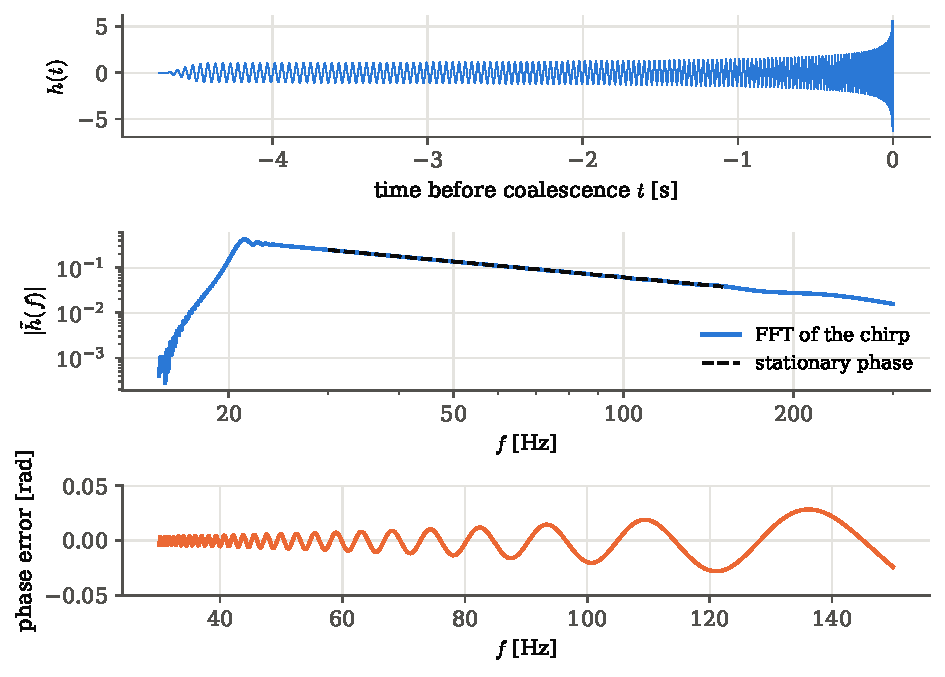
\includegraphics[width=0.85\linewidth]{figures/chT2/spa_check.pdf}
\caption{The stationary-phase formula against a direct FFT. Top: the chirp in time, its amplitude and frequency rising towards coalescence. Middle: $\lvert\tilde h\rvert$ from the FFT and from \eqref{T2a:eq:spa}, which fall together as $f^{-7/6}$ in the band; the FFT drops at $20$\,Hz, where the signal starts. Bottom: the phase of the FFT minus the predicted $-\Psi(f)$, a few hundredths of a radian.}
\label{T2a:fig:spa-check}
\end{figure}

\paragraph{Example: two phases that are easy to confuse.}
Papers on environments plot the \emph{time-domain} phase left before merger, $\Phi(f)=2\pi\int_t^{t_c}f\,\dd t$, which is $2\pi$ times the number of cycles \cite{Coogan2022}, \cite[eq.~(48)]{Kim2023}. The Fisher matrix uses the Fourier phase $\Psi(f)$. For the Newtonian chirp, \eqref{T2a:eq:Ncyc} with $f_2\to\infty$ gives $\Phi(f)=\tfrac1{16}x$, with $x\equiv(\pi G\mathcal Mf/c^3)^{-5/3}$. With $t_c=\phi_c=0$, the phase at time $t_f$ is $\phi(t_f)=-\Phi(f)$, so
\begin{align*}
  \Psi(f)+\frac\pi4
  &\eqby{1}2\pi f\,t_f-\phi(t_f)
  \eqby{2}-2\pi f\,\tau(f)+\Phi(f)
  \eqby{3}-\frac{10}{256}\,x+\frac{16}{256}\,x
  =\frac{3}{128}\,x .
\end{align*}
\begin{explain}
  \item Definition of $\Psi$ in \eqref{T2a:eq:spa}.
  \item $t_f=-\tau(f)$ and $\phi(t_f)=-\Phi(f)$, since the phase still to come is $\Phi(f)$ and the phase reaches $\phi_c=0$ at $t_c$.
  \item $2\pi f\tau=2\pi\cdot\tfrac5{256}(G\mathcal M/c^3)^{-5/3}\pi^{-8/3}f^{-5/3}=\tfrac{10}{256}x$, and $\tfrac1{16}=\tfrac{16}{256}$.
\end{explain}
So $\Psi$ carries $\tfrac38$ of the time-domain phase, because the term $2\pi f t_f$ removes the part a shift of the arrival time can absorb. For the EMRI four years before the ISCO, $\Phi\approx2\pi\times\TwEmriNcyc$ while the $f$-dependent part of $\Psi$ is about three eighths of that. Both phases are correct; they answer different questions, and a dephasing quoted in one cannot be compared with a phase error in the other without this conversion.

\paragraph{Where this is used.}
The waveform \eqref{T2a:eq:hf} with the phase \eqref{T2a:eq:psiN} is the signal model of \cref{10b:sec:signal-model}, extended there by the post-Newtonian terms derived in \cref{T2g:sec:pn}. The fact that $t_c$ and $\phi_c$ enter $\Psi$ only as $2\pi ft_c-\phi_c$ is what lets \cref{10b:sec:phase-time} search all arrival times with one inverse Fourier transform. The relations \eqref{T2a:eq:psi-derivs} are the bridge from any change of the sweep rate to a change of the phase, used in \cref{10b:sec:env-derive}, and \cref{10b:sec:two-phases} carries out the conversion between the two kinds of phase.
\section{Corrections to the phase: post-Newtonian orders and the ppE form}
\label{T2g:sec:pn}

The chirp of \cref{T2a:sec:chirp} rests on Newton's law of gravity and on the quadrupole formula, both of which are the first term of an expansion in $v/c$. Far from merger that is excellent. Near the ISCO the orbital speed is $v=c/\sqrt6\approx0.4c$, and the corrections are tens of per cent. Even far from merger, a correction of a few per cent to the rate of the inspiral is not small in the only currency that matters for a matched filter: over a million cycles, a few per cent is tens of thousands of cycles, and a template that slips by one cycle has lost the signal (\cref{T2a:sec:chirp}). Other physics acts the same way. A cloud of dark matter, a disc of gas, or a departure from general relativity each changes how fast the binary loses energy, by a fraction that depends on the frequency.

So the question is: \emph{if the binding energy or the radiated power differs from its Newtonian value by a small fractional term, how does that change the Fourier phase $\Psi(f)$, and which power of $f$ does each kind of correction produce?} The answer is one rule. A correction that scales as $v^p$ relative to the Newtonian term adds to $\Psi$ a term proportional to $f^{(p-5)/3}$, with a coefficient we can compute once and for all. General-relativistic corrections have $p=2,3,4,\dots$; environments and some modifications of gravity have negative $p$. The rule turns the whole zoo of corrections into one family, $\delta\Psi=\beta u^b$, which is the form the forecast of \cref{ch:10} uses.

\subsection{The expansion parameter}

Measure the speed of the orbit by the observable wave frequency. For a Newtonian circular orbit, Kepler's law gives the orbital speed $v_{\rm orb}=r\omega=(GM\omega)^{1/3}$, and with $\omega=\pi f$ from \eqref{T2g:eq:twice},
\begin{equation}
  v\equiv\Big(\frac{\pi GMf}{c^3}\Big)^{1/3}=\frac{v_{\rm orb}}{c},\qquad x\equiv v^2 ,
  \label{T2g:eq:v}
\end{equation}
with $M=m_1+m_2$ the total mass. A correction of relative size $v^{2k}$ is called \newterm{$k$PN} (post-Newtonian) order, so $1$PN means $v^2$, $1.5$PN means $v^3$. Using $f$ rather than the orbital radius $r$ is deliberate: $r$ depends on the coordinates used to describe the strong-field region, while the frequency of the wave at the detector does not \cite[Sec.~III A]{CutlerFlanagan1994}. Two mass combinations will appear: the \newterm{symmetric mass ratio} $\eta=m_1m_2/M^2=\mu/M$ \unpack{$\tfrac14$ for equal masses, about $m_2/m_1$ when one body is much lighter}, and the chirp mass, $\mathcal M=\eta^{3/5}M$. The reduced frequency of the Newtonian phase is then
\begin{equation}
  u\equiv\frac{\pi G\mathcal Mf}{c^3}=\eta^{3/5}v^3,\qquad u^{-5/3}=\eta^{-1}v^{-5}.
  \label{T2g:eq:u}
\end{equation}

\subsection{From the energy and the flux to the phase}

\emph{Inputs.} The orbit is still circular and evolves slowly, so energy balance $\dd E/\dd t=-\mathcal F$ holds at each moment, with $E(v)$ the binding energy and $\mathcal F(v)$ the power radiated, now allowed to carry corrections. In the Newtonian limit, by \eqref{T2a:eq:Ef} and \eqref{T2a:eq:Pf} written in terms of $v$,
\begin{equation}
  E_{\rm N}=-\tfrac12\mu c^2v^2,\qquad
  \mathcal F_{\rm N}=\frac{32}{5}\frac{c^5}{G}\,\eta^2v^{10}.
  \label{T2g:eq:EFnewton}
\end{equation}
(For $E$: $\tfrac12\mu(\pi GMf)^{2/3}=\tfrac12\mu c^2v^2$. For the power: $u^{10/3}=\eta^2v^{10}$ by \eqref{T2g:eq:u}.)

\emph{The time.} Energy balance gives $\dd t=-\dd E/\mathcal F=-(\dd E/\dd v)\,\dd v/\mathcal F$. Write the corrections to $\dd E/\dd v$ and $\mathcal F$ together as one bracket,
\begin{equation}
  \frac{\dd t}{\dd v}=-\frac{E'(v)}{\mathcal F(v)}
  =-\frac{E_{\rm N}'}{\mathcal F_{\rm N}}\,\big[1+c_pv^p+\dots\big]
  =\frac{5GM}{32c^3\eta}\,v^{-9}\big[1+c_pv^p+\dots\big],
  \label{T2g:eq:dtdv}
\end{equation}
because $-E_{\rm N}'/\mathcal F_{\rm N}=\mu c^2v\big/\big(\tfrac{32}{5}\tfrac{c^5}{G}\eta^2v^{10}\big)=\tfrac{5}{32}\tfrac{G\mu}{c^3\eta^2}v^{-9}$ and $\mu=\eta M$. The bracket may contain several terms; each acts separately at first order, so we follow one, $c_pv^p$.

\emph{The phase.} From \eqref{T2a:eq:psi-derivs}, $\dd\Psi/\dd f=2\pi t(f)=2\pi t_c-2\pi\tau(f)$, where $\tau=t_c-t$ is the time left. So $\Psi=2\pi ft_c-\phi_c-\tfrac\pi4-2\pi\int^f\tau\,\dd f'$, with the integration constants named as in \eqref{T2a:eq:psiN}. We need $\tau$ as a function of $v$, and $\dd f$ in terms of $\dd v$:
\begin{align}
  \tau(v)&\eqby{1}\int_v^\infty\frac{\dd t}{\dd v'}\,\dd v'
  \eqby{2}\frac{5GM}{32c^3\eta}\Big[\frac{v^{-8}}{8}+c_p\frac{v^{p-8}}{8-p}\Big],
  \qquad \dd f\eqby{3}\frac{3c^3v^2}{\pi GM}\,\dd v,\nonumber\\
  -2\pi\int\tau\,\dd f
  &\eqby{4}-\frac{15}{16\eta}\int\Big[\frac{v^{-6}}{8}+c_p\frac{v^{p-6}}{8-p}\Big]\dd v
  \eqby{5}\frac{15}{16\eta}\Big[\frac{v^{-5}}{40}+c_p\frac{v^{p-5}}{(8-p)(5-p)}\Big]\nonumber\\
  &\eqby{6}\frac{3}{128\,\eta\,v^5}\Big[1+\frac{40\,c_p}{(8-p)(5-p)}\,v^p\Big].
  \label{T2g:eq:rule}
\end{align}
\begin{explain}
  \item The time left is the integral of $\dd t$ from the current speed to the end, where $v\to\infty$ formally, as in \eqref{T2a:eq:tau}.
  \item $\int_v^\infty v'^{q}\dd v'=v^{q+1}/(-q-1)$ for $q<-1$; here $q=-9$ and $q=p-9$, which needs $p<8$.
  \item $f=c^3v^3/(\pi GM)$ from \eqref{T2g:eq:v}.
  \item Multiply: $2\pi\cdot\tfrac{5GM}{32c^3\eta}\cdot\tfrac{3c^3}{\pi GM}=\tfrac{15}{16\eta}$, and $v^{-8}v^2=v^{-6}$.
  \item $\int v^{q}\dd v=v^{q+1}/(q+1)$: for $q=-6$ this is $-v^{-5}/5$ and for $q=p-6$ it is $-v^{p-5}/(5-p)$, which needs $p\neq5$. The two minus signs cancel the one in front; the constants of integration join $\phi_c$.
  \item Factor out the Newtonian term: $\tfrac{15}{16}\cdot\tfrac1{40}=\tfrac{3}{128}$, and the ratio of the two coefficients is $\tfrac{1/((8-p)(5-p))}{1/40}$.
\end{explain}
For $p=0$ only the Newtonian term is left, $\tfrac{3}{128}\eta^{-1}v^{-5}=\tfrac3{128}u^{-5/3}$, which is \eqref{T2a:eq:psiN} again. A correction $c_pv^p$ in the rate of the inspiral therefore becomes a phase term
\begin{equation}
  \delta\Psi=\frac{3}{128}\,u^{-5/3}\,\frac{40\,c_p}{(8-p)(5-p)}\,v^p\ \propto\ f^{(p-5)/3}.
  \label{T2g:eq:power-rule}
\end{equation}
At $p=5$ the integral in step (5) is a logarithm instead of a power; this is why the $2.5$PN term of the phase contains $\ln f$.

\subsection{The 1PN and 1.5PN phase}

\emph{The inputs from general relativity.} The binding energy to $1$PN order and the flux to $1.5$PN order are standard results, which Cutler and Flanagan quote in terms of the orbital radius $r$ in a particular coordinate system \cite[eqs.~(35)--(37)]{CutlerFlanagan1994}, \cite{Blanchet2014}. In units $G=c=1$,
\begin{equation}
  \Omega^2=\frac{M}{r^3}\Big[1-(3-\eta)\frac Mr\Big],\qquad
  E=-\frac{\mu M}{2r}\Big[1-\frac{7-\eta}{4}\frac Mr\Big],
\end{equation}
and the flux is $\tfrac{32}{5}\eta^2(M\Omega)^{10/3}[1-(\tfrac{1247}{336}+\tfrac{35}{12}\eta)\tfrac Mr+4\pi(\tfrac Mr)^{3/2}]$. The first expression is the square of their eq.~(35), to the same order. The $4\pi$ is the \newterm{tail}: part of the outgoing wave scatters off the curved spacetime around the binary on its way out, and the scattered part interferes with the rest.

\emph{Rewritten in $v$.} With $v^2=(M\Omega)^{2/3}$,
\begin{align}
  v^2&\eqby{1}\frac Mr\Big[1-(3-\eta)\frac Mr\Big]^{1/3}\eqby{2}\frac Mr\Big[1-\Big(1-\frac\eta3\Big)\frac Mr\Big],
  \qquad \frac Mr\eqby{3}v^2\Big[1+\Big(1-\frac\eta3\Big)v^2\Big],\nonumber\\
  E&\eqby{4}-\frac{\mu}{2}v^2\Big[1+\Big(1-\frac\eta3\Big)v^2-\frac{7-\eta}{4}v^2\Big]
  \eqby{5}-\frac{\mu}{2}v^2\Big[1-\frac{9+\eta}{12}v^2\Big].
  \label{T2g:eq:E1PN}
\end{align}
\begin{explain}
  \item $(M\Omega)^{2/3}=(M^2/r^3)^{1/3}[\dots]^{1/3}=(M/r)[\dots]^{1/3}$.
  \item $(1-\epsilon)^{1/3}=1-\epsilon/3$.
  \item Invert to first order: if $v^2=y(1-ky)$ then $y=v^2(1+kv^2)$.
  \item Insert into $E$; in the $1$PN bracket $M/r=v^2$ is enough.
  \item $1-\tfrac\eta3-\tfrac74+\tfrac\eta4=-\tfrac34-\tfrac{\eta}{12}=-\tfrac{9+\eta}{12}$.
\end{explain}
The flux is already written with $(M\Omega)^{10/3}=v^{10}$ in front, and inside its bracket $M/r=v^2$ to the order needed. So, restoring $c$,
\begin{equation}
  E'(v)=-\mu c^2v\Big[1-\frac{9+\eta}{6}v^2\Big],\qquad
  \mathcal F=\frac{32}{5}\frac{c^5}{G}\eta^2v^{10}\Big[1-\Big(\frac{1247}{336}+\frac{35}{12}\eta\Big)v^2+4\pi v^3\Big],
\end{equation}
where $E'$ comes from differentiating $v^2-\tfrac{9+\eta}{12}v^4$ to $2v-\tfrac{9+\eta}{3}v^3$.

\emph{The bracket of \eqref{T2g:eq:dtdv}.} Dividing,
\begin{align}
  \frac{E'/E_{\rm N}'}{\mathcal F/\mathcal F_{\rm N}}
  &\eqby{1}\Big[1-\frac{9+\eta}{6}v^2\Big]\Big[1+\Big(\frac{1247}{336}+\frac{35}{12}\eta\Big)v^2-4\pi v^3\Big]
  \eqby{2}1+\Big(\frac{743}{336}+\frac{11}{4}\eta\Big)v^2-4\pi v^3,
\end{align}
\begin{explain}
  \item $1/(1-\epsilon)=1+\epsilon$ to first order, applied to the flux bracket.
  \item Multiply out to order $v^3$: $\tfrac{1247}{336}-\tfrac96=\tfrac{1247-504}{336}=\tfrac{743}{336}$ and $\tfrac{35}{12}-\tfrac16=\tfrac{33}{12}=\tfrac{11}{4}$.
\end{explain}
so $c_2=\tfrac{743}{336}+\tfrac{11}{4}\eta$ and $c_3=-4\pi$. The rule \eqref{T2g:eq:rule} gives the factors $\tfrac{40}{6\cdot3}=\tfrac{20}{9}$ for $p=2$ and $\tfrac{40}{5\cdot2}=4$ for $p=3$:
\begin{equation}
  \Psi(f)=2\pi ft_c-\phi_c-\frac\pi4+\frac{3}{128}\,u^{-5/3}\Big[1+\frac{20}{9}\Big(\frac{743}{336}+\frac{11}{4}\eta\Big)x-16\pi x^{3/2}\Big],
  \label{T2g:eq:psi-pn}
\end{equation}
with $x=v^2$. This is Cutler and Flanagan's restricted post-Newtonian phase \cite[eq.~(42)]{CutlerFlanagan1994}, in our sign convention, and it is the waveform used in \cref{10b:sec:signal-model}. The same bracket inverted gives the chirp rate, $\dot f\propto1-(\tfrac{743}{336}+\tfrac{11}4\eta)x+4\pi x^{3/2}$, their eq.~(38). The symmetric mass ratio $\eta$ appears for the first time at $1$PN: it is the post-Newtonian terms that let the data separate $m_1$ from $m_2$ once $\mathcal M$ is known.

\paragraph{Example: how many cycles each term is worth.}
Count cycles instead of phase: the number of wave cycles is $N=\int f\,\dd t=\int f(\dd t/\dd v)\,\dd v$, and with \eqref{T2g:eq:dtdv} and $f=c^3v^3/(\pi GM)$,
\begin{equation}
  N(v_1,v_2)=\frac{5}{32\pi\eta}\int_{v_1}^{v_2}v^{-6}\big[1+c_2v^2+c_3v^3\big]\dd v
  =\frac{5}{32\pi\eta}\Big[\frac{v^{-5}}{5}+c_2\frac{v^{-3}}{3}+c_3\frac{v^{-2}}{2}\Big]_{v_2}^{v_1}.
\end{equation}
The first term is \eqref{T2a:eq:Ncyc} again. The script \pyname{14_pn_cycles.py} evaluates the three terms separately (\cref{T2g:fig:pn-cycles}). For a pair of $1.4\,M_\odot$ neutron stars observed from $10$\,Hz to the ISCO by a ground-based detector, the Newtonian term gives $\TwPNNsN$ cycles, the $1$PN term $\TwPNNsOne$ and the tail $\TwPNNsOnefive$, in agreement with the counts Blanchet tabulates for the same band (about $1.6\times10^{4}$, $441$ and $-211$) \cite{Blanchet2014}. For the book's intermediate mass-ratio benchmark in its last four years ($v$ from $\TwPNImrivone$ to $\TwPNImrivtwo$), the counts are $\TwPNImriN$, $\TwPNImriOne$ and $\TwPNImriOnefive$; for the EMRI, $\TwPNEmriN$, $\TwPNEmriOne$ and $\TwPNEmriOnefive$. Tens of thousands of cycles from each correction: no template can leave them out. Even the GW150914-like binary crossing the LISA band years before merger, at $v\approx0.03$, gains $\TwPNGWOne$ cycles from the $1$PN term.

\begin{figure}[htbp]
\centering
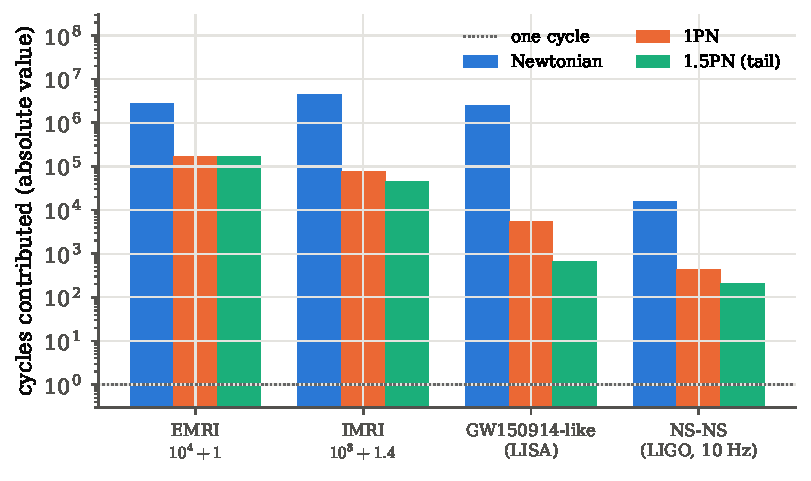
\includegraphics[width=0.82\linewidth]{figures/chT2/pn_cycles.pdf}
\caption{Number of wave cycles contributed by the Newtonian term and by the $1$PN and $1.5$PN (tail) corrections, for the four binaries named below the bars, each in its observation window. The dotted line marks one cycle, the slip that ruins a matched filter. Every correction is worth hundreds to hundreds of thousands of cycles.}
\label{T2g:fig:pn-cycles}
\end{figure}

\begin{pitfall}[Post-Newtonian series for extreme mass ratios]
For the EMRI the $1$PN and $1.5$PN counts are almost equal and opposite, each about six per cent of the total. Near the ISCO, $v\approx0.4$, successive terms of the series shrink only slowly, so truncating it at $1.5$PN leaves an error of many cycles. Research templates for extreme mass ratios therefore come from black-hole perturbation theory (the small body moving in the exact geometry of the large one, corrected by its own field) rather than from the post-Newtonian series; the power-law structure derived here is used to describe small \emph{changes} to such a template, not the template itself.
\end{pitfall}

\subsection{Every correction is a power of the frequency: the ppE form}

The rule \eqref{T2g:eq:power-rule} applies to any small correction that scales as a power of $v$, whatever its origin. In terms of the reduced frequency $u$ of \eqref{T2g:eq:u}, $v^p=\eta^{-p/5}u^{p/3}$, so a correction of relative order $v^p$ becomes
\begin{equation}
  \delta\Psi=\beta\,u^{b},\qquad b=\frac{p-5}{3},
  \label{T2g:eq:ppe-rule}
\end{equation}
with all the constants, including the powers of $\eta$, in $\beta$. For the general-relativistic terms $p=2k$ at $k$PN order, so $b=(2k-5)/3$: $-1$ at $1$PN, $-2/3$ at $1.5$PN, $-1/3$ at $2$PN. A term that grows \emph{at low frequency} faster than the Newtonian $-\tfrac53$ must come from a correction with $p<0$, one that is relatively more important when the binary is wide and slow. Yunes and Pretorius proposed to test general relativity with exactly this family: the \newterm{parameterised post-Einsteinian} (ppE) waveform
\begin{equation}
  \tilde h(f)=\tilde h_{\rm GR}(f)\,\big(1+\alpha u^{a}\big)\,e^{-i\beta u^{b}},
  \label{T2g:eq:ppe}
\end{equation}
in our sign convention, where $(\alpha,a)$ change the amplitude and $(\beta,b)$ the phase, and general relativity is $\alpha=\beta=0$ \cite[eq.~(1)]{YunesPretorius2009}. (Yunes and Pretorius write the powers of $(\pi G\mathcal Mf/c^3)^{1/3}$, so each of their exponents is three times ours.) The environments of \cref{T2a:sec:forces} fit into the same family: a dark-matter spike adds a drag whose power relative to the radiated one falls as $f^{-n}$, which by \eqref{T2g:eq:ppe-rule} with $p=-3n$ is $b=-\tfrac53-n$, \eqref{T2a:eq:ppe}.

\paragraph{Example: dipole radiation, $b=-7/3$.}
In some alternatives to general relativity, such as the Brans--Dicke theory, a compact body carries a scalar ``charge'' that is not proportional to its mass, and the binary emits dipole radiation as well. By the estimate at the end of \cref{T2g:sec:quadrupole}, dipole power relative to quadrupole power scales as $(v/c)^{-2}$. So $\mathcal F=\mathcal F_{\rm N}(1+Bv^{-2})$, the bracket of \eqref{T2g:eq:dtdv} gains $-Bv^{-2}$, $p=-2$, and $b=(-2-5)/3=-\tfrac73$: Yunes and Pretorius's Brans--Dicke case \cite{YunesPretorius2009}. A ``$-1$PN'' term, it is largest at the lowest frequencies, which is why a long, slow inspiral in the LISA band is a sensitive test of it.

\paragraph{Example: a massive graviton, $b=-1$.}
If the graviton had a mass $m_g$, waves of energy $hf$ would travel at the group velocity $v_g=c\sqrt{1-m_g^2c^4/(hf)^2}\approx c\,[1-m_g^2c^4/(2h^2f^2)]$, and low frequencies would arrive late. Over a distance $D$ the delay is $\Delta t(f)=(D/c)\,m_g^2c^4/(2h^2f^2)=Dc/(2\lambda_g^2f^2)$, with $\lambda_g=h/(m_gc)$ the graviton's Compton wavelength. The arrival time of frequency $f$ is what the slope of the Fourier phase measures, $\dd\Psi/\dd f=2\pi t(f)$ by \eqref{T2a:eq:psi-derivs}, so
\begin{align}
  \delta\Psi(f)&\eqby{1}2\pi\int\Delta t(f)\,\dd f
  \eqby{2}2\pi\,\frac{Dc}{2\lambda_g^2}\int f^{-2}\,\dd f
  \eqby{3}-\frac{\pi Dc}{\lambda_g^2}\,f^{-1}+\text{const},
\end{align}
\begin{explain}
  \item Integrate the extra delay once, as in \eqref{T2a:eq:psiN}.
  \item Insert $\Delta t(f)$.
  \item $\int f^{-2}\dd f=-f^{-1}$; the constant joins $\phi_c$.
\end{explain}
a term $\propto f^{-1}$, so $b=-1$, the ppE massive-graviton case \cite{YunesPretorius2009}. It has the same exponent as the $1$PN term, which is why a graviton mass and the mass ratio are partly degenerate in a fit, a correlation \cref{10b:sec:corr} meets in another guise.

\begin{figure}[htbp]
\centering
\begin{tikzpicture}[scale=1.0]
  \def\s{2.6}
  \draw[->,thick] ({-4.1*\s},0) -- ({0.6*\s},0) node[right,lbl] {$b$};
  \foreach \b/\t in {-4/{$-4$},-3/{$-3$},-2/{$-2$},-1/{$-1$},0/{$0$}}{
    \draw ({\b*\s},0.08) -- ({\b*\s},-0.08);
    \node[lbl,below] at ({\b*\s},-0.08) {\t};}
  \foreach \b/\lab/\h in {-1.6667/{Newtonian\\ $-5/3$}/0.95,-1/{1PN}/0.55,-0.6667/{1.5PN}/1.05,-0.3333/{2PN}/0.55}{
    \fill[formblue] ({\b*\s},0) circle (2pt);
    \draw[formblue,thin] ({\b*\s},0) -- ({\b*\s},{\h-0.18});
    \node[lbl,formblue,align=center,anchor=south] at ({\b*\s},{\h-0.2}) {\lab};}
  \foreach \b/\lab/\h/\dx in {-3.7778/{friction in a\\ $7/3$ spike}/-0.75/0,-2.3333/{dipole\\ radiation}/-0.75/0,-1/{graviton\\ mass}/-0.75/0.3}{
    \fill[bdryred] ({\b*\s},0) circle (2pt);
    \draw[bdryred,thin] ({\b*\s},0) -- ({(\b+\dx)*\s},{\h+0.3});
    \node[lbl,bdryred,align=center,anchor=north] at ({(\b+\dx)*\s},{\h+0.3}) {\lab};}
  \node[lbl,align=left,anchor=west] at ({-4.1*\s},1.3) {general relativity:};
  \node[lbl,align=left,anchor=west] at ({-4.1*\s},-1.75) {environments and modified gravity:};
\end{tikzpicture}
\caption{The exponent $b$ of the term $\beta u^b$ that each effect adds to the Fourier phase. General-relativistic corrections (blue, above the line) sit at $b=(2k-5)/3$ and climb towards zero as the PN order $k$ grows. Effects that matter most when the binary is wide and slow (red, below) have $b<-5/3$: dipole radiation at $-7/3$, dynamical friction in a dark-matter spike of slope $7/3$ at $-34/9$. A graviton mass lands on the same exponent as the $1$PN term.}
\label{T2g:fig:exponents}
\end{figure}

\begin{keyidea}[A correction $v^p$ becomes a phase term $f^{(p-5)/3}$]
If the binding energy or the radiated power differs from its Newtonian value by a relative term $c_pv^p$, the Fourier phase gains $\delta\Psi=\tfrac{3}{128}u^{-5/3}\cdot\tfrac{40c_p}{(8-p)(5-p)}v^p\propto u^{(p-5)/3}$. General relativity's $k$PN terms have $p=2k$; environments and dipole radiation have $p<0$. Any such effect is a ppE term $\beta u^b$, with the exponent $b$ naming the physics and $\beta$ its strength.
\end{keyidea}

\paragraph{Where this is used.}
The phase \eqref{T2g:eq:psi-pn} is the signal model of \cref{10b:sec:signal-model}, and the exponents of its terms are what make its Fisher matrix in \cref{10b:sec:fisher-structure} a set of weighted averages of powers of $f$. The rule \eqref{T2g:eq:ppe-rule} is the general form behind \cref{10b:sec:env-derive}, where an environment is a power law in the phase, and behind \cref{10b:sec:sigma-b}, which computes the error on $\beta$ for every exponent $b$ at once; the specific exponents of dark-matter environments are derived in \cref{T2a:sec:forces}.
\section{What LISA measures, and what hides the signal}
\label{T2a:sec:lisa}

LISA will be three spacecraft flying in a triangle $L=2.5$ million kilometres on a side, trailing the Earth around the Sun (\cref{T2a:fig:lisa-triangle}). Each spacecraft shields test masses that fall freely, and laser links measure the distance between test masses on different spacecraft. By \eqref{T2g:eq:displacement} a gravitational wave of strain $h$ changes an arm's length by about $\tfrac12hL$. For $h\sim10^{-20}$ that is about $10^{-11}$\,m, ten picometres over millions of kilometres. The whole instrument is designed around measuring such changes, and its noise is the floor under which a signal can hide.

For the statistics, LISA is summarised by a single function. The data are the signal plus noise, $d=h(\params)+n$. For a given $\params$, the likelihood of \cref{10b:sec:noise-fd} asks how plausible the particular noise realisation $n=d-h(\params)$ is, and for stationary Gaussian noise that plausibility is set, one Fourier component at a time, by the noise power at that frequency. So the likelihood weights each frequency by the inverse of the noise power there, and the Fisher matrix of \cref{ch:10} inherits that weight. The question is therefore physical: \emph{at each frequency, how large is the noise, where does it come from, and how large would a gravitational wave have to be to produce the same output?} The answer is the sensitivity curve $S_n(f)$ \cite{Robson2019}.

\subsection{A noise spectrum as a physical quantity}

The statistics of a noise spectrum, how it describes the correlations of a stationary random process and how it is estimated from data, is developed in \cref{10b:sec:noise-fd,10b:sec:welch}. Here we need only what it means physically. Pass the noise $n(t)$ through a narrow filter that keeps only frequencies between $f$ and $f+\Delta f$, and measure the mean square of what comes out. The \newterm{one-sided power spectral density} $S_n(f)$ is that mean square divided by $\Delta f$:
\begin{equation}
  \big\langle n^2\big\rangle_{[f,f+\Delta f]}=S_n(f)\,\Delta f,\qquad
  \big\langle n^2\big\rangle=\int_0^\infty S_n(f)\,\dd f .
  \label{T2g:eq:band-power}
\end{equation}
``One-sided'' means that only positive frequencies are counted, the negative ones having been folded onto them as in \cref{T2a:sec:spa}. Its square root, the \newterm{amplitude spectral density} $\sqrt{S_n}$, is in units of the measured quantity per $\sqrt{\rm Hz}$: a displacement noise of $15$\,pm\,Hz$^{-1/2}$ means that, averaged over one second (a band of about $1$\,Hz), the length reading scatters by about $15$\,pm. Two noises from independent causes add in power, $S=S_1+S_2$, because the mean square of a sum of uncorrelated terms is the sum of their mean squares. And if a noise in one quantity is converted into another by a linear, frequency-dependent factor, as a force becomes a displacement, the spectrum is multiplied by the squared modulus of that factor.

\subsection{From test-mass jitter and photon counting to strain sensitivity}

\paragraph{The two instrumental noises.}
Two processes limit the arm-length measurement \cite[eqs.~(10)--(11)]{Robson2019}:
\begin{align}
  P_{\rm OMS}(f)&=(1.5\times10^{-11}\,{\rm m})^2\Big[1+\Big(\frac{2\,{\rm mHz}}{f}\Big)^4\Big]\ {\rm Hz}^{-1},\nonumber\\
  P_{\rm acc}(f)&=(3\times10^{-15}\,{\rm m\,s^{-2}})^2\Big[1+\Big(\frac{0.4\,{\rm mHz}}{f}\Big)^2\Big]\Big[1+\Big(\frac{f}{8\,{\rm mHz}}\Big)^4\Big]\ {\rm Hz}^{-1}.\label{T2a:eq:lisa-noise}
\end{align}
The first is \newterm{optical metrology} noise, the error with which the laser interferometry reads the length of one link: about $15$\,pm\,Hz$^{-1/2}$, flat in frequency apart from a rise below $2$\,mHz. The second is \newterm{acceleration noise}: stray forces on the free-falling test masses, from impacts of residual gas molecules, electrostatic and magnetic forces on the slightly charged and magnetised masses, and the pressure of thermal radiation from their housing, push each of them around by about $3\times10^{-15}$\,m\,s$^{-2}$\,Hz$^{-1/2}$.

\paragraph{Example: where 15 picometres comes from.}
Most of the metrology noise is photon \emph{shot noise}, the graininess of light, and its size follows from counting photons. A laser of about $2$\,W leaves one spacecraft through a telescope of diameter $D\approx0.3$\,m. Diffraction spreads the beam by an angle $\theta\approx\lambda/D=1.064\,\mu{\rm m}/0.3\,{\rm m}=3.5\times10^{-6}$, so after $L=2.5\times10^9$\,m the spot has a radius of about $\theta L\approx9$\,km, and the receiving telescope, of radius $0.15$\,m, catches a fraction of order $(0.15/9000)^2\approx3\times10^{-10}$ of it: a received power $P_r\approx6\times10^{-10}$\,W. Each photon carries $hc/\lambda=1.9\times10^{-19}$\,J, so about $\dot N=P_r\lambda/hc\approx3\times10^9$ photons arrive per second. A phase measured by counting $N$ photons is uncertain by $1/\sqrt N$ radians, the Poisson fluctuation of the count (\cref{ch:02}), and a phase $\delta\varphi$ is a length $\lambda\,\delta\varphi/2\pi$. Per second of averaging,
\begin{equation*}
  \delta x\approx\frac{\lambda}{2\pi}\frac{1}{\sqrt{\dot N\times1\,{\rm s}}}
  =\frac{1.06\times10^{-6}\,{\rm m}}{2\pi}\times\frac{1}{\sqrt{3\times10^9}}\approx3\times10^{-12}\,{\rm m},
\end{equation*}
a few picometres per $\sqrt{\rm Hz}$, the same order as the $15$\,pm\,Hz$^{-1/2}$ allocated to all the metrology noise together. Counting statistics does not depend on how fast the signal varies, so shot noise is white in displacement. The arm length helps the signal ($\delta L\propto L$) but hurts the light budget ($P_r\propto L^{-2}$); $2.5$ million kilometres is a compromise between the two.

\paragraph{Why acceleration noise is divided by $(2\pi f)^4$.}
A force noise becomes a displacement noise by integrating twice in time, and integration in time is division by frequency:
\begin{align}
  \ddot x(t)=a(t)
  \;\;\Rightarrow\;\;
  (2\pi i f)^2\tilde x(f)\eqby{1}\tilde a(f)
  \;\;\Rightarrow\;\;
  P_x(f)\eqby{2}\frac{P_a(f)}{(2\pi f)^4}.
  \label{T2g:eq:acc-disp}
\end{align}
\begin{explain}
  \item Fourier transform with the book's convention \eqref{T2g:eq:fourier}: each time derivative becomes a factor $2\pi if$.
  \item The spectrum is multiplied by the squared modulus of the conversion factor; $\lvert(2\pi if)^2\rvert^2=(2\pi f)^4$.
\end{explain}
A random push of given strength moves a mass far if it keeps pushing the same way for a long time, that is at low frequency, and hardly at all if it reverses quickly. So acceleration noise is harmless at high frequency and dominates at low frequency, rising as $f^{-4}$ in power.

\paragraph{Adding up the noise in one Michelson channel.}
Follow one arm, with test mass A at the vertex spacecraft and test mass B at the far one, and let $x_A(t)$, $x_B(t)$ be their random displacements along the arm (positive in the direction from A to B). Light leaves A at $t-2L/c$, is sent back from B at $t-L/c$ and returns to A at $t$. The measured round-trip length changes by
\begin{align}
  \delta\ell(t)
  &\eqby{1}\big[x_B(t-L/c)-x_A(t-2L/c)\big]+\big[x_B(t-L/c)-x_A(t)\big],\nonumber\\
  \tilde{\delta\ell}(f)
  &\eqby{2}2e^{-2\pi ifL/c}\,\tilde x_B-\big(1+e^{-4\pi ifL/c}\big)\tilde x_A,\nonumber\\
  P_{\delta\ell}
  &\eqby{3}4P_x+\big\lvert1+e^{-4\pi ifL/c}\big\rvert^2P_x
  \eqby{4}4P_x+4\cos^2\!\Big(\frac{2\pi fL}{c}\Big)P_x
  =4\Big(1+\cos^2\frac{f}{f_*}\Big)P_x .
\end{align}
\begin{explain}
  \item The outward leg is lengthened by B's displacement when the light arrives and shortened by A's when it left; the return leg likewise, with A's displacement at the end.
  \item A delay by $T$ multiplies a Fourier transform by $e^{-2\pi ifT}$, as in a time shift (\cref{10b:sec:phase-time}).
  \item A and B jitter independently with the same spectrum $P_x$, so their contributions add in power; $\lvert2e^{-i\cdot}\rvert^2=4$.
  \item $\lvert1+e^{-i\theta}\rvert^2=2+2\cos\theta=4\cos^2(\theta/2)$ with $\theta=4\pi fL/c$, and $2\pi fL/c=f/f_*$.
\end{explain}
The far mass counts four times because the light touches it twice at the same moment; the vertex mass counts at two moments $2L/c$ apart, which add in step at low frequency and cancel when the round trip is half a period. A Michelson channel is the difference of two such arms, and in LISA each arm has its own test mass at the vertex, so the acceleration noise of the channel is $8(1+\cos^2f/f_*)P_{\rm acc}/(2\pi f)^4$: sixteen units at low frequency. The metrology noise enters once per one-way link, two links per arm, two arms: $4P_{\rm OMS}$. The signal in the same channel is the round-trip difference $2L\,D_{ij}h_{ij}$ of \cref{T2g:sec:detector}, so dividing the noise by $(2L)^2$ expresses it as an equivalent strain:
\begin{equation}
  P_n(f)=\frac{4P_{\rm OMS}+8\big(1+\cos^2\frac{f}{f_*}\big)\frac{P_{\rm acc}}{(2\pi f)^4}}{4L^2}
  =\frac{1}{L^2}\Big[P_{\rm OMS}+2\Big(1+\cos^2\frac{f}{f_*}\Big)\frac{P_{\rm acc}}{(2\pi f)^4}\Big],
  \label{T2g:eq:Pn}
\end{equation}
which is Robson et al.'s eq.~(12), with its ``four contributions from the optical metrology noise and sixteen from the test mass acceleration noise'' \cite{Robson2019}.

\paragraph{The noise that is cancelled before it is counted.}
There is a third noise, far larger than both: the laser's own frequency jitter. Even a stabilised laser wanders in frequency by about one part in $10^{13}$ per $\sqrt{\rm Hz}$, and a Michelson interferometer is immune to that only if its two arms are equally long, so that both beams carry the same old laser light back to be compared. LISA's arms differ by about one per cent, some $2.5\times10^7$\,m, so the jitter would appear as a length noise of order $10^{-13}\times2.5\times10^7\,{\rm m}\approx2.5\,\mu$m per $\sqrt{\rm Hz}$, some $10^5$ times the signal. LISA therefore records every one-way link separately and, on the ground, adds the records with time shifts chosen so that the laser noise cancels exactly, synthesising an equal-arm Michelson after the fact. This is \newterm{time-delay interferometry}. What survives it is the test-mass and metrology noise counted above.

\paragraph{From the noise in the channel to the sensitivity curve.}
$P_n$ is the noise of one channel expressed as a strain, but a real wave is not optimally oriented: on average over the sky and polarisation the channels respond to only a fraction $R(f)$ of the wave's power, $\tfrac{3}{10}$ at low frequency for the two channels together and falling above $f_*$ (\cref{T2g:sec:detector}). It is conventional to move that factor from the signal onto the noise \cite[eq.~(2)]{Robson2019}: the \newterm{sensitivity curve} is the noise divided by the response. With the fit $R(f)=\tfrac3{10}/[1+0.6(f/f_*)^2]$, checked in \cref{T2g:fig:response},
\begin{equation}
  S_n(f)=\frac{P_n(f)}{R(f)}
  =\frac{10}{3L^2}\Big[P_{\rm OMS}(f)+2\Big(1+\cos^2\frac{f}{f_*}\Big)\frac{P_{\rm acc}(f)}{(2\pi f)^4}\Big]\Big[1+\frac{6}{10}\Big(\frac{f}{f_*}\Big)^2\Big]+S_c(f).
  \label{T2a:eq:Sn}
\end{equation}
At $f\ll f_*$ the factor $2(1+\cos^2)$ is $4$, the simpler form of Robson et al.'s eq.~(1) \cite{Robson2019}; the code uses the full factor.

\paragraph{The Galactic confusion noise.}
The last term in \eqref{T2a:eq:Sn} is not instrumental. Our Galaxy contains tens of millions of binaries of white dwarfs radiating at millihertz frequencies. A four-year observation divides the frequency axis into bins of width $1/T\approx8$\,nHz, and below a few millihertz there are more binaries than bins. They cannot be separated from one another, and their sum acts as an extra noise \cite[Sec.~1]{Robson2019}:
\begin{equation}
  S_c(f)=A\,f^{-7/3}\,e^{-f^{\alpha}+\beta f\sin(\kappa f)}\,\big[1+\tanh(\gamma(f_k-f))\big]\ {\rm Hz}^{-1},
\end{equation}
with $A=9\times10^{-45}$ and, for four years, $(\alpha,\beta,\kappa,\gamma,f_k)=(0.138,-221,521,1680,1.13\,{\rm mHz})$ \cite[eq.~(14)]{Robson2019}.

\emph{Why $f^{-7/3}$?} The power law follows from the chirp. Suppose white-dwarf binaries form at a steady rate at low frequency and then drift upwards in frequency at the rate $\dot f\propto f^{11/3}$ of \eqref{T2a:eq:fdot}. In a steady state the number of binaries crossing any frequency per unit time is the same at every $f$, like a steady flow of traffic: $(\dd N/\dd f)\,\dot f=\text{const}$, so $\dd N/\dd f\propto f^{-11/3}$. Where binaries move quickly they are few. Each binary contributes a mean-square strain $\propto A^2\propto f^{4/3}$, by \eqref{T2g:eq:amp}. Summing the power of all binaries in a band, as \eqref{T2g:eq:band-power} sums the power of a noise,
\begin{equation}
  S_c(f)\propto\frac{\dd N}{\dd f}\,A^2\propto f^{-11/3}\,f^{4/3}=f^{-7/3}.
\end{equation}
The other factors of the fit describe where this simple picture fails. Above the knee $f_k$ there is less than about one binary per bin, so the binaries can be fitted and subtracted one by one, and the $\tanh$ switches the confusion off. The longer LISA observes, the finer the bins, the more binaries are resolved, and the lower the knee moves (it is $2.58$\,mHz after six months). The confusion noise is also not stationary: it rises and falls during the year as the antenna pattern of \cref{T2g:sec:detector} sweeps across the Galactic centre. The fit is its average.

\begin{workdef}[sensitivity curve]
The \newterm{sensitivity curve} $S_n(f)$ is the one-sided noise power spectral density of the detector divided by its sky- and polarisation-averaged response, plus any unresolved foreground \unpack{the noise expressed as the strain power a gravitational wave would need to produce the same output}. \emph{Operationally:} in the inner product $(a\,|\,b)=4\,\mathrm{Re}\int\tilde a\tilde b^*/S_n\,\dd f$ use $S_n(f)$ of \eqref{T2a:eq:Sn} together with the angle-averaged waveform $\tilde h=\sqrt{4/5}\,\mathcal Af^{-7/6}e^{-i\Psi}$.
\end{workdef}

\Cref{T2a:fig:lisa-noise} shows the three pieces. Acceleration noise dominates below $\TwfAccOms$\,mHz (by hand: setting $P_{\rm OMS}=4P_{\rm acc}/(2\pi f)^4$ without the correction factors gives $(2\pi f)^4=4\times9\times10^{-30}/2.25\times10^{-22}=1.6\times10^{-7}\,{\rm s^{-4}}$, i.e.\ $f=3.2$\,mHz). The confusion noise exceeds the instrument between $\TwfConfLo$ and $\TwfConfHi$\,mHz. Above $f_*=\Twfstar$\,mHz the falling response makes the curve rise again. The best sensitivity, $\sqrt{S_n}=\TwASDmin\,{\rm Hz^{-1/2}}$, is reached near $\TwfASDmin$\,mHz.

\begin{figure}[htbp]
\centering
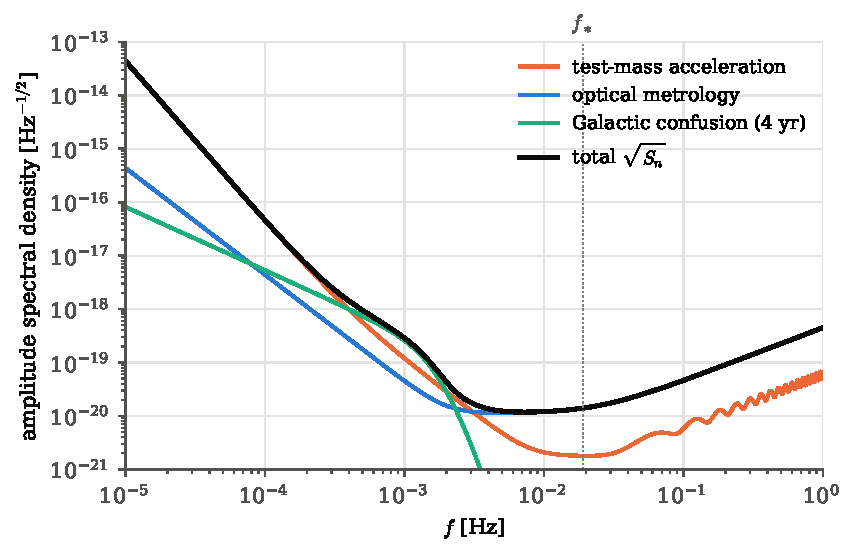
\includegraphics[width=0.8\linewidth]{figures/chT2/lisa_noise.pdf}
\caption{The LISA sensitivity curve and its three ingredients, as amplitude spectral densities $\sqrt{S}$. Test-mass acceleration noise falls steeply with frequency, optical metrology noise is flat and then rises above $f_*$ (dotted) where the arms respond less, and the Galactic confusion noise fills the gap around a millihertz. The thick curve is the total used throughout the book.}
\label{T2a:fig:lisa-noise}
\end{figure}

The curve is a short function in \pyname{lib_lisa.py}:

\pyfile[firstline=100,lastline=111,firstnumber=100]{code/chT2/lib_lisa.py}{The three pieces of $S_n(f)$ and their sum}

\noindent The factor \pyname{resp} on line 102 is $\tfrac{10}{3L^2}[1+0.6(f/f_*)^2]$, the conversion from displacement noise to strain sensitivity. Line 103 is the metrology term of \eqref{T2a:eq:Sn}, line 104 the acceleration term with its $f^{-4}$ and the full factor $2(1+\cos^2)$, and line 105 hands back the confusion fit. \pyname{Sn_lisa} adds the three; with \pyname{confusion=False} it is the instrument alone.

\subsection{How loud is a source?}

With the noise in hand, the signal-to-noise ratio of \cref{ch:00} is $\rho^2=(h\,|\,h)=4\int\lvert\tilde h\rvert^2/S_n\,\dd f$. For the angle-averaged waveform of \cref{T2a:sec:spa}, $\lvert\tilde h\rvert^2=\tfrac45\mathcal A^2f^{-7/3}$ (with $\mathcal A$ the amplitude of \eqref{T2a:eq:hf}), and it is useful to rewrite the integral so that a plot shows it:
\begin{equation}
  \rho^2\eqby{1}\frac{16}{5}\int\frac{\mathcal A^2f^{-7/3}}{S_n(f)}\,\dd f
  \eqby{2}\int\Big(\frac{h_c(f)}{h_n(f)}\Big)^2\dd\ln f,
  \qquad h_c\equiv2f\lvert\tilde h(f)\rvert,\quad h_n\equiv\sqrt{fS_n(f)} .
  \label{T2a:eq:snr}
\end{equation}
\begin{explain}
  \item Insert $\lvert\tilde h\rvert^2=\tfrac45\mathcal A^2f^{-7/3}$; $4\cdot\tfrac45=\tfrac{16}{5}$ \cite[eq.~(18)]{Robson2019}.
  \item $4\lvert\tilde h\rvert^2\dd f/S_n=(2f\lvert\tilde h\rvert)^2/(fS_n)\cdot\dd f/f$, and $\dd f/f=\dd\ln f$.
\end{explain}
Both $h_c$, the \newterm{characteristic strain}, and $h_n$ are dimensionless. On log--log axes the height of a source's track above the noise curve shows how much signal-to-noise ratio each decade of frequency contributes. A track below the curve can still be detected if it is long enough, because the integral adds up many frequencies.

\paragraph{Example: the three benchmark sources.}
The script \pyname{03_lisa_noise.py} evaluates \eqref{T2a:eq:snr} on the four-year stretch of each binary of \cref{T2a:sec:chirp}. Kim et al.\ place the EMRI at $D_L=203$\,Mpc, where five years of data give a signal-to-noise ratio of about $15$ \cite[Sec.~III F]{Kim2023}. For our four years we place it where $\rho=\TwEmriSNR$, which is $D_L=\TwEmriDL$\,Mpc, close to their distance. The IMRI at $75$\,Mpc, the distance out to which Coogan et al.\ find dark-matter environments measurable \cite{Coogan2022}, reaches $\rho=\TwImriSNR$ between $\TwImriffouryr$\,mHz and the $1$\,Hz end of the band. The GW150914-like binary at $410$\,Mpc reaches only $\rho=\TwGWlikeSNR$: on its own LISA would not claim it, which is why such sources are studied together with ground-based detectors. \Cref{T2a:fig:lisa-tracks} shows the tracks. Since $h_c\propto f\cdot f^{-7/6}=f^{-1/6}$, each inspiral is an almost flat line that ends where the binary reaches its ISCO or leaves the band.

\begin{figure}[htbp]
\centering
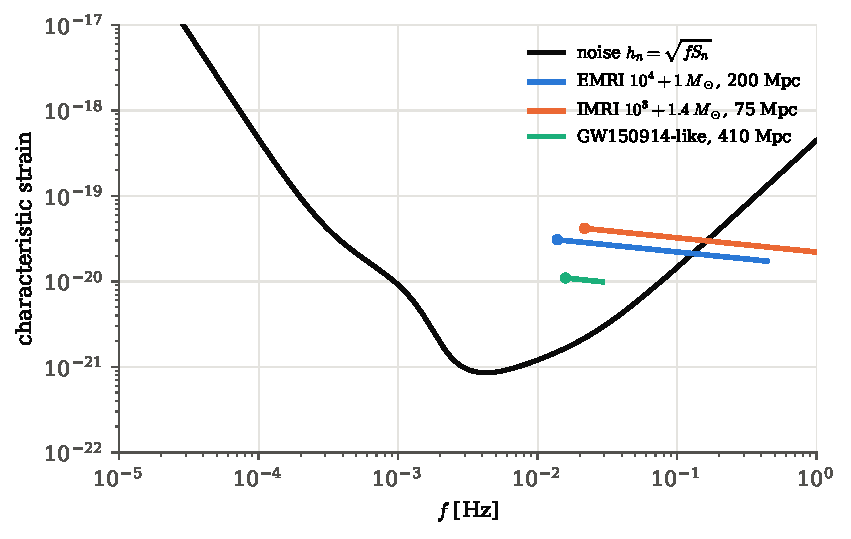
\includegraphics[width=0.8\linewidth]{figures/chT2/lisa_tracks.pdf}
\caption{Characteristic strain of the three benchmark binaries during four years of observation (dots mark the start), over the LISA noise amplitude $h_n=\sqrt{fS_n}$. The squared ratio of the two curves, integrated over $\ln f$, is the squared signal-to-noise ratio \eqref{T2a:eq:snr}. The EMRI and the IMRI sit well above the noise over a decade or more of frequency; the GW150914-like binary is short and sits only several times above it.}
\label{T2a:fig:lisa-tracks}
\end{figure}

\begin{pitfall}[Three conventions for one curve]
The literature plots $\sqrt{P_n}$ (noise only), $\sqrt{S_n}=\sqrt{P_n/R}$ (noise over response) and $h_n=\sqrt{fS_n}$ (dimensionless), and quotes the low-frequency response as $3/10$ (two channels) or $3/20$ (one) \cite[Sec.~1]{Robson2019}. Each is correct with the matching signal. Pair $S_n$ with the angle-averaged waveform $\sqrt{4/5}\,\mathcal Af^{-7/6}$, or $P_n$ with the full detector response, and never mix them: a mismatch changes every signal-to-noise ratio and Fisher error by a constant factor that nothing else in the calculation will reveal.
\end{pitfall}

\paragraph{Where this is used.}
The curve \eqref{T2a:eq:Sn} is the $S_n(f)$ of the noise-weighted inner product of \cref{10b:sec:noise-fd}, and with it of every likelihood, matched filter and Fisher matrix in \cref{ch:10}; \cref{10b:sec:robson} checks it against the published figure, and \cref{10b:sec:benchmark} uses the signal-to-noise ratio \eqref{T2a:eq:snr} to place the benchmark source. In real data $S_n$ is not known in advance but estimated, which is the subject of \cref{10b:sec:welch,10b:sec:psd}; the non-stationary confusion noise is one reason why that estimate is hard.
\section{The symbols, where they come from, and where they are used}
\label{T2g:sec:symbols}

Every gravitational-wave object that \cref{ch:10} takes as given has a short derivation above. The table that follows gives each symbol in a few words, the equation or section where it was derived, and the part of \cref{ch:10} in which it does its work. The rows follow the chain of \cref{T2a:fig:roadmap}: the wave, the source, the chirp, the frequency domain, the corrections, the detector and its noise.

\begin{table}[htbp]
\centering
\footnotesize
\renewcommand{\arraystretch}{1.18}
\begin{tabularx}{\linewidth}{@{}>{\raggedright\arraybackslash}p{2.35cm} >{\raggedright\arraybackslash}X >{\raggedright\arraybackslash}p{2.1cm} >{\raggedright\arraybackslash}p{2.5cm}@{}}
\toprule
symbol & meaning & derived in & used in \cref{ch:10} \\
\midrule
$h_+$, $h_\times$ & the two polarisations of a wave, in the transverse plane & \eqref{T2g:eq:tt} & \S\ref{10b:sec:detection} \\
$\delta L/L=\tfrac12h_{aa}$ & fractional change of an arm's length, read by light travel time & \eqref{T2g:eq:displacement}, \eqref{T2g:eq:arm} & \S\ref{10b:sec:detection} \\
$F_+$, $F_\times$; $D_{ij}$ & antenna patterns: weights of the polarisations in the detector output; detector tensor & \eqref{T2g:eq:response}, \eqref{T2g:eq:Fplus} & \S\ref{10b:sec:detection} \\
$\tfrac15$, $\tfrac3{20}$, $R=\tfrac3{10}$ & sky- and polarisation-averaged response: right-angle, one $60^\circ$ channel, two LISA channels & \eqref{T2g:eq:one-fifth}, \eqref{T2g:eq:sixty} & \S\ref{10b:sec:robson} \\
$\tfrac45$ & inclination average of a circular binary's signal power & \eqref{T2g:eq:four-fifths} & \S\ref{10b:sec:robson}, \S\ref{10b:sec:benchmark} \\
$f_*=c/2\pi L$ & transfer frequency; response falls as $f^{-2}$ above it & \eqref{T2g:eq:transfer} & \S\ref{10b:sec:robson} \\
$M$, $\mu$, $\eta$ & total mass, reduced mass, symmetric mass ratio $\mu/M$ & \S\ref{T2g:sec:quadrupole}, \eqref{T2g:eq:v} & \S\ref{10b:sec:signal-model} \\
$\mathcal M$ & chirp mass $\mu^{3/5}M^{2/5}$, the mass the Newtonian signal depends on & \eqref{T2g:eq:amp}, \eqref{T2a:eq:Pf} & \S\ref{10b:sec:signal-model}, \S\ref{10b:sec:fisher-examples} \\
$f=2f_{\rm orb}$ & wave frequency, twice the orbital one & \eqref{T2g:eq:twice} & throughout \\
$A$; $\mathcal A$ & time-domain amplitude; Fourier amplitude of $\tilde h=\mathcal Af^{-7/6}e^{-i\Psi}$ & \eqref{T2g:eq:amp}, \eqref{T2a:eq:hf} & \S\ref{10b:sec:matched-filter}, \S\ref{10b:sec:signal-model} \\
$\iota$, $\psi$ & inclination of the orbit; polarisation angle & \eqref{T2g:eq:hpc}, \eqref{T2g:eq:Fplus} & \S\ref{10b:sec:robson} \\
$P_{\rm GW}$, $E(f)$ & radiated power; orbital binding energy & \eqref{T2g:eq:power-binary}, \eqref{T2a:eq:Ef} & \S\ref{10b:sec:env-derive} \\
$\dot f$ & chirp rate $\tfrac{96}{5}\pi^{8/3}(G\mathcal M/c^3)^{5/3}f^{11/3}$ & \eqref{T2a:eq:fdot} & \S\ref{10b:sec:env-derive} \\
$\tau(f)$, $N$, $f_{\rm ISCO}$ & time left to coalescence; number of cycles; end of the inspiral & \eqref{T2a:eq:tau}, \eqref{T2a:eq:Ncyc}, \eqref{T2a:eq:fisco} & \S\ref{10b:sec:benchmark} \\
$t_c$, $\phi_c$ & time and phase of coalescence: nuisance parameters & \eqref{T2g:eq:phit}, \S\ref{T2g:sec:tc-phic} & \S\ref{10b:sec:phase-time}, \S\ref{10b:sec:fisher-examples} \\
$\tilde h(f)$ & Fourier transform, $\int h\,e^{-2\pi ift}\dd t$; $\tilde h(-f)=\tilde h(f)^*$ & \eqref{T2g:eq:fourier}, \eqref{T2g:eq:reality} & \S\ref{10b:sec:noise-fd} \\
$\Psi(f)$ & Fourier phase of the chirp, from the stationary-phase approximation & \eqref{T2a:eq:spa}, \eqref{T2a:eq:psiN} & \S\ref{10b:sec:signal-model} \\
$\Psi'=2\pi t(f)$, $\Psi''=2\pi/\dot f$ & what the phase knows: arrival time and chirp rate & \eqref{T2a:eq:psi-derivs} & \S\ref{10b:sec:env-derive} \\
$\Phi(f)$ & time-domain phase still to come; $\Psi$ carries $\tfrac38$ of it & \S\ref{T2a:sec:spa} (example) & \S\ref{10b:sec:two-phases} \\
$v$, $x$, $u$ & PN parameter $(\pi GMf/c^3)^{1/3}$, $x=v^2$, reduced frequency $\pi G\mathcal Mf/c^3$ & \eqref{T2g:eq:v}, \eqref{T2g:eq:u} & \S\ref{10b:sec:signal-model} \\
1PN, 1.5PN terms & corrections $\tfrac{20}{9}(\tfrac{743}{336}+\tfrac{11}4\eta)x$ and $-16\pi x^{3/2}$ & \eqref{T2g:eq:psi-pn} & \S\ref{10b:sec:signal-model} \\
$\beta$, $b$ & ppE amplitude and exponent of a phase term $\beta u^b$; $b=(p-5)/3$ & \eqref{T2g:eq:ppe-rule}, \eqref{T2a:eq:ppe} & \S\ref{10b:sec:env}, \S\ref{10b:sec:sigma-b} \\
$S_n(f)$ & one-sided noise spectrum divided by the response: the sensitivity curve & \eqref{T2g:eq:band-power}, \eqref{T2a:eq:Sn} & \S\ref{10b:sec:noise-fd}, \S\ref{10b:sec:robson} \\
$P_{\rm OMS}$, $P_{\rm acc}$, $S_c$ & metrology, test-mass acceleration and Galactic confusion noise & \eqref{T2a:eq:lisa-noise}, \eqref{T2g:eq:Pn} & \S\ref{10b:sec:robson} \\
$h_c$, $h_n$, $\rho$ & characteristic strain, noise amplitude, signal-to-noise ratio & \eqref{T2a:eq:snr} & \S\ref{10b:sec:benchmark} \\
\bottomrule
\end{tabularx}
\caption{The gravitational-wave symbols of \cref{ch:10}: what each one is, the equation or section that derives it, and the section of \cref{ch:10} that uses it.}
\label{T2g:tab:symbols}
\end{table}

The rows are links of one chain of reasoning. Einstein's equation for a weak field gave a wave with two polarisations that changes distances by $\tfrac12h$. Mass and momentum conservation made the quadrupole the first source of such waves, and the energy they carry made a binary chirp. The stationary-phase approximation turned the chirp into a Fourier-domain template whose phase is a sum of powers of $f$, two of whose terms, $2\pi ft_c-\phi_c$, are nuisances, and whose other terms, Newtonian, post-Newtonian or environmental, carry the physics. The detector added its geometry, through $F_+$, $F_\times$ and the averages $\tfrac45$ and $\tfrac3{10}$, and its noise, through $S_n(f)$. Nothing in the list is a convention to be taken on trust; each entry can be recomputed from the two physical inputs of \cref{T2g:sec:wave} and Newton's law of gravity.

\begin{recap}
\begin{itemize}[itemsep=1pt]
  \item A weak gravitational wave is a transverse, traceless ripple $h_{ij}$ moving at $c$, with two polarisations $h_+$, $h_\times$ that mix under rotations with twice the angle; it changes the distance between free masses by $\delta L/L=\tfrac12h_{ij}\hat n_i\hat n_j$, a travelling tidal squeeze.
  \item Conservation of mass and momentum forbids monopole and dipole radiation, so slow sources radiate through $\ddot Q_{ij}$: $h^{\rm TT}_{ij}=(2G/c^4r)[\ddot Q_{ij}]^{\rm TT}$ and $P=(G/5c^5)\langle\dddot Q\dddot Q\rangle$. A circular binary radiates at $f=2f_{\rm orb}$ with amplitude $4(G\mathcal M)^{5/3}(\pi f)^{2/3}/(c^4D)$ and power $\tfrac{32}{5}(G/c^5)\mu^2r^4\omega^6$.
  \item A detector outputs $h=F_+h_++F_\times h_\times$. Averages: $\tfrac15$ over sky and polarisation, $\tfrac34$ for $60^\circ$ arms, $\tfrac3{10}$ for LISA's two channels, $\tfrac45$ over inclination. Above $f_*=c/(2\pi L)=19$\,mHz the response falls as $f^{-2}$.
  \item Energy balance gives the chirp $\dot f\propto\mathcal M^{5/3}f^{11/3}$; integrating it gives the time to merger, the number of cycles and the phase, with the nuisance constants $t_c$ and $\phi_c$.
  \item The stationary-phase approximation, a Taylor expansion of the phase plus a Fresnel integral, gives $\tilde h=\mathcal Af^{-7/6}e^{-i\Psi}$ with $\Psi'=2\pi t(f)$ and $\Psi''=2\pi/\dot f$, checked against an FFT.
  \item A relative correction $v^p$ to the energy or flux adds $\propto f^{(p-5)/3}$ to $\Psi$: the 1PN and 1.5PN terms of the standard template, dipole radiation at $b=-7/3$, a graviton mass at $b=-1$, environments at $b=-5/3-n$, all of the ppE form $\beta u^b$.
  \item LISA's noise is shot noise (flat in displacement) and test-mass acceleration noise (divided by $(2\pi f)^4$), counted through the round trips of a Michelson channel and divided by the response to give $S_n(f)$, plus the $f^{-7/3}$ confusion noise of unresolved Galactic binaries.
\end{itemize}
\end{recap}

\providecommand{\TwEmriMc}{}\renewcommand{\TwEmriMc}{39.81}
\providecommand{\TwEmrifisco}{}\renewcommand{\TwEmrifisco}{0.4397}
\providecommand{\TwEmriffouryr}{}\renewcommand{\TwEmriffouryr}{13.84}
\providecommand{\TwEmriNcyc}{}\renewcommand{\TwEmriNcyc}{2.787\times10^{6}}
\providecommand{\TwEmriadiab}{}\renewcommand{\TwEmriadiab}{6.839\times10^{-5}}
\providecommand{\TwImriMc}{}\renewcommand{\TwImriMc}{19.39}
\providecommand{\TwImrifisco}{}\renewcommand{\TwImrifisco}{4.391}
\providecommand{\TwImriffouryr}{}\renewcommand{\TwImriffouryr}{21.7}
\providecommand{\TwImriNcyc}{}\renewcommand{\TwImriNcyc}{4.382\times10^{6}}
\providecommand{\TwImriadiab}{}\renewcommand{\TwImriadiab}{9.550\times10^{-4}}
\providecommand{\TwGWMc}{}\renewcommand{\TwGWMc}{28.1}
\providecommand{\TwGWfFive}{}\renewcommand{\TwGWfFive}{15.83}
\providecommand{\TwGWfOne}{}\renewcommand{\TwGWfOne}{28.94}
\providecommand{\TwGWNcyc}{}\renewcommand{\TwGWNcyc}{2.534\times10^{6}}
\providecommand{\TwSpaAmpErr}{}\renewcommand{\TwSpaAmpErr}{3.655}
\providecommand{\TwSpaPhaseRms}{}\renewcommand{\TwSpaPhaseRms}{0.01296}
\providecommand{\TwSpaPsiBand}{}\renewcommand{\TwSpaPsiBand}{168.4}
\providecommand{\TwSpaDuration}{}\renewcommand{\TwSpaDuration}{4.729}
\providecommand{\Twfstar}{}\renewcommand{\Twfstar}{19.09}
\providecommand{\TwASDmin}{}\renewcommand{\TwASDmin}{1.178\times10^{-20}}
\providecommand{\TwfASDmin}{}\renewcommand{\TwfASDmin}{7.256}
\providecommand{\TwfAccOms}{}\renewcommand{\TwfAccOms}{3.077}
\providecommand{\TwfConfLo}{}\renewcommand{\TwfConfLo}{0.4101}
\providecommand{\TwfConfHi}{}\renewcommand{\TwfConfHi}{1.908}
\providecommand{\TwEmriDL}{}\renewcommand{\TwEmriDL}{199.8}
\providecommand{\TwEmriSNR}{}\renewcommand{\TwEmriSNR}{14}
\providecommand{\TwImriSNR}{}\renewcommand{\TwImriSNR}{12.1}
\providecommand{\TwGWlikeSNR}{}\renewcommand{\TwGWlikeSNR}{3.89}
\providecommand{\Twconc}{}\renewcommand{\Twconc}{13.49}
\providecommand{\Twrtwohundred}{}\renewcommand{\Twrtwohundred}{9.82}
\providecommand{\TwrsNFW}{}\renewcommand{\TwrsNFW}{0.7279}
\providecommand{\Twdeltac}{}\renewcommand{\Twdeltac}{9.39\times10^{4}}
\providecommand{\Twrhos}{}\renewcommand{\Twrhos}{0.01184}
\providecommand{\Twrsp}{}\renewcommand{\Twrsp}{3.759}
\providecommand{\Twrhosp}{}\renewcommand{\Twrhosp}{2.269}
\providecommand{\Twrhpc}{}\renewcommand{\Twrhpc}{9.571\times10^{-10}}
\providecommand{\TwrsgOverRh}{}\renewcommand{\TwrsgOverRh}{4.5\times10^{4}}
\providecommand{\Twrhosg}{}\renewcommand{\Twrhosg}{1.190\times10^{11}}
\providecommand{\TwrorbFour}{}\renewcommand{\TwrorbFour}{30.09}
\providecommand{\TwrorbIsco}{}\renewcommand{\TwrorbIsco}{3}
\providecommand{\TwrhoOrb}{}\renewcommand{\TwrhoOrb}{2.279\times10^{16}}
\providecommand{\TwrhoBoost}{}\renewcommand{\TwrhoBoost}{2.279\times10^{18}}
\providecommand{\TwmuParticle}{}\renewcommand{\TwmuParticle}{2.003\times10^{-12}}
\providecommand{\TwmuCompton}{}\renewcommand{\TwmuCompton}{6.681\times10^{-15}}
\providecommand{\TwfeqA}{}\renewcommand{\TwfeqA}{4.181}
\providecommand{\TwdPhiFourA}{}\renewcommand{\TwdPhiFourA}{1.302\times10^{5}}
\providecommand{\TwbexpA}{}\renewcommand{\TwbexpA}{-4.333}
\providecommand{\TwfeqB}{}\renewcommand{\TwfeqB}{8.883}
\providecommand{\TwdPhiFourB}{}\renewcommand{\TwdPhiFourB}{1.325\times10^{6}}
\providecommand{\TwbexpB}{}\renewcommand{\TwbexpB}{-4}
\providecommand{\TwfeqC}{}\renewcommand{\TwfeqC}{16.75}
\providecommand{\TwdPhiFourC}{}\renewcommand{\TwdPhiFourC}{5.191\times10^{6}}
\providecommand{\TwbexpC}{}\renewcommand{\TwbexpC}{-3.778}
\providecommand{\TwclosedVsNum}{}\renewcommand{\TwclosedVsNum}{1.343\times10^{-13}}
\providecommand{\TwPLerrFour}{}\renewcommand{\TwPLerrFour}{35.35}
\providecommand{\TwfeqD}{}\renewcommand{\TwfeqD}{24.26}
\providecommand{\TwdPhiFourD}{}\renewcommand{\TwdPhiFourD}{8.937\times10^{6}}
\providecommand{\TwbexpD}{}\renewcommand{\TwbexpD}{-3.667}
\providecommand{\TwCwSmallErr}{}\renewcommand{\TwCwSmallErr}{0.8254}
\providecommand{\TwaccRatioThirty}{}\renewcommand{\TwaccRatioThirty}{0.02222}
\providecommand{\TwaccRatioThree}{}\renewcommand{\TwaccRatioThree}{0.2222}
\providecommand{\TwffourImri}{}\renewcommand{\TwffourImri}{21.7}
\providecommand{\TwlnLambdaC}{}\renewcommand{\TwlnLambdaC}{3.286}
 
\section{Dark matter around black holes}
\label{T2a:sec:dm}

The signal model of \cref{T2a:sec:spa,T2g:sec:pn} describes a binary in empty space: a chirp whose Fourier phase $\Psi(f)$ \eqref{T2a:eq:psiN} is fixed by the chirp mass $\mathcal M$ \eqref{T2a:eq:Pf} and the coalescence constants $t_c$, $\phi_c$ (\cref{T2g:sec:tc-phic}), and to which any extra physics adds a power of the frequency, $\beta u^b$ \eqref{T2g:eq:ppe-rule}. This section and the next supply the extra physics that the forecasts of \cref{ch:10} test. Here we ask where dark matter around a black hole comes from and how dense it becomes; \cref{T2a:sec:forces} finds the forces it exerts on the orbit and the exponent $b$ they produce.

Near the Sun, dark matter has a density of about $0.01\,M_\odot\,{\rm pc}^{-3}$. Spread at that density over a sphere the size of the EMRI orbit of \cref{T2a:sec:chirp}, about $30$ Schwarzschild radii of a $10^4\,M_\odot$ hole or $3\times10^{-8}$\,pc, it amounts to $\tfrac43\pi(3\times10^{-8})^3\times0.01\approx10^{-24}\,M_\odot$. No orbit could feel that. A survey of environmental effects on inspirals concludes exactly this: for most sources, galactic dark matter at ordinary densities is irrelevant \cite[Sec.~IX]{Barausse2014}. If a gravitational wave is to show dark matter, something must have packed it around the black hole at densities some eighteen orders of magnitude higher. The black hole itself can do it. So the question is: \emph{how does a black hole that grows at the centre of a dark-matter halo rearrange the dark matter around it, and how dense does it become where the companion orbits?}

\subsection{The halo far away}

Far from any black hole, simulations of cold dark matter find the \newterm{Navarro--Frenk--White} (NFW) profile
\begin{equation}
  \rho_{\rm NFW}(r)=\frac{\rho_s}{(r/r_s)(1+r/r_s)^2},
  \label{T2a:eq:nfw}
\end{equation}
which falls as $r^{-1}$ inside the scale radius $r_s$ and as $r^{-3}$ outside it \cite{NFW1996}, \cite[eq.~(1)]{NFW1997}. The inner $r^{-1}$ is called a \newterm{cusp}. A halo has no sharp edge, so it is labelled by the mass inside a conventional one. The reference density is the \newterm{critical density} $\rho_{\rm crit}=3H_0^2/(8\pi G)$, the mean density at which a universe expanding at today's rate $H_0$ would be spatially flat, about $1.3\times10^{-7}\,M_\odot\,{\rm pc}^{-3}$ for $h=0.674$. The edge $r_{200}$ is the radius within which the mean density of the halo is $200\rho_{\rm crit}$, and $M_{200}$ is the mass inside it. Since that mass is $200\rho_{\rm crit}$ times the volume $\tfrac43\pi r_{200}^3$, the mass fixes the edge, $r_{200}=[3M_{200}/(800\pi\rho_{\rm crit})]^{1/3}$. The second label is the concentration $c=r_{200}/r_s$, which then fixes $r_s=r_{200}/c$. What remains is $\rho_s$, and it follows from the enclosed mass:
\begin{align}
  M(<r)&\eqby{1}4\pi\rho_sr_s^3\int_0^{r/r_s}\frac{x\,\dd x}{(1+x)^2}
  \eqby{2}4\pi\rho_sr_s^3\Big[\ln\Big(1+\frac r{r_s}\Big)-\frac{r/r_s}{1+r/r_s}\Big],\nonumber\\
  \rho_s&\eqby{3}\rho_{\rm crit}\,\frac{200}{3}\,\frac{c^3}{\ln(1+c)-c/(1+c)}\equiv\rho_{\rm crit}\,\delta_c .\label{T2a:eq:nfw-mass}
\end{align}
\begin{explain}
  \item $M=\int_0^r4\pi r'^2\rho\,\dd r'$ with $x=r'/r_s$; the factor $x^2/x$ leaves $x$.
  \item $\frac{x}{(1+x)^2}=\frac1{1+x}-\frac1{(1+x)^2}$ integrates to $\ln(1+x)+\frac1{1+x}-1=\ln(1+x)-\frac x{1+x}$.
  \item Evaluate step (2) at $r=r_{200}=cr_s$ and set it equal to $200\rho_{\rm crit}\cdot\tfrac43\pi r_{200}^3$:
        $4\pi\rho_sr_s^3\big[\ln(1+c)-\tfrac{c}{1+c}\big]=\tfrac{800\pi}{3}\rho_{\rm crit}\,c^3r_s^3$. The factor $r_s^3$ cancels, and dividing by $4\pi[\dots]$ gives $\rho_s$ \cite[eq.~(2)]{NFW1997}.
\end{explain}
Take a dwarf-galaxy halo with $M_{200}=10^8\,M_\odot$. The concentration--mass relation of Correa et al.\ at redshift zero \cite[eq.~(19)]{Correa2015} gives $c=\Twconc$, and then $r_{200}=\Twrtwohundred$\,kpc, $r_s=\TwrsNFW$\,kpc, $\delta_c=\Twdeltac$ and $\rho_s=\Twrhos\,M_\odot\,{\rm pc}^{-3}$ (with $h=0.674$). These are ordinary galactic numbers. The interesting physics is inside, where the black hole dominates.

\subsection{The spike: what slow growth of a black hole does}

Suppose a black hole of mass $M$ grows at the centre of the cusp slowly, over many orbital periods of the surrounding dark matter. Each dark-matter particle feels the potential deepen gradually and moves inward to a tighter orbit. Dark matter piles up around the hole. The simplest orbits, circles, already give the answer.

\emph{Inputs.} (i) Physical: the growth is \newterm{adiabatic} \unpack{slow compared with the orbital period of the dark matter at the radius considered}, so a particle on a circular orbit stays on a circular orbit and keeps its angular momentum, which is conserved in any spherical potential. (ii) Physical: orbits do not cross. Every circular orbit shrinks, but an orbit that started inside another stays inside it, so the shells keep their order, and the mass inside each orbit is the same before and after. (iii) Physical: before the growth the gravity at radius $r_i$ comes from the dark matter inside it; afterwards the gravity at the new radius $r_f$ comes from the hole alone. The last input needs a word. The compressed dark matter inside $r_f$ weighs the same $M_i(r_i)$ it weighed before the growth, and the radii of interest are those where that is much less than $M$; there the hole's pull dominates and the dark matter's own pull is a small correction.

\emph{The mass inside the old orbit.} For an initial cusp $\rho_i=\rho_0(r/r_0)^{-\gamma_i}$ with $\gamma_i<3$, adding up thin shells gives
\[
  M_i(r_i)=\int_0^{r_i}4\pi r^2\rho_0\Big(\frac{r}{r_0}\Big)^{-\gamma_i}\dd r=\frac{4\pi\rho_0r_0^{\gamma_i}}{3-\gamma_i}\,r_i^{3-\gamma_i}\propto r_i^{3-\gamma_i}.
\]

\emph{Same angular momentum, smaller orbit.} Equating the angular momentum before and after, and then following the mass of a shell to its new radius,
\begin{align}
  G\,M_i(r_i)\,r_i&\eqby{1}G\,M\,r_f
  \;\;\Rightarrow\;\; r_f\eqby{2}\frac{M_i(r_i)\,r_i}{M}\propto r_i^{4-\gamma_i},\nonumber\\
  \rho_f(r_f)&\eqby{3}\rho_i(r_i)\,\frac{r_i^2}{r_f^2}\,\frac{\dd r_i}{\dd r_f}
  \eqby{4}\frac{\rho_i(r_i)}{4-\gamma_i}\,\frac{r_i^3}{r_f^3}
  \propto r_i^{3-\gamma_i}\,r_f^{-3}
  \eqby{5}r_f^{\frac{3-\gamma_i}{4-\gamma_i}-3}
  =r_f^{-\frac{9-2\gamma_i}{4-\gamma_i}} .\label{T2a:eq:spike-slope}
\end{align}
\begin{explain}
  \item For a circular orbit $v^2=GM_{\rm enc}/r$, so the squared angular momentum per unit mass is $L^2=r^2v^2=GM_{\rm enc}\,r$. Before the growth $M_{\rm enc}=M_i(r_i)$; after it $M_{\rm enc}=M$ by input (iii). $L^2$ is the same by input (i).
  \item Solve for $r_f$ and use $M_i(r_i)\propto r_i^{3-\gamma_i}$.
  \item By input (ii) the shell between $r_i$ and $r_i+\dd r_i$ becomes the shell between $r_f$ and $r_f+\dd r_f$ with the same mass: $4\pi r_i^2\rho_i\,\dd r_i=4\pi r_f^2\rho_f\,\dd r_f$. Divide by $4\pi r_f^2\dd r_f$.
  \item From step (2), $\dd r_f/\dd r_i=(4-\gamma_i)\,r_f/r_i$, so $\dd r_i/\dd r_f=r_i/[(4-\gamma_i)r_f]$.
  \item Step (2) inverted, $r_i\propto r_f^{1/(4-\gamma_i)}$, and $\rho_i\propto r_i^{-\gamma_i}$. The exponent is $\frac{3-\gamma_i}{4-\gamma_i}-3=\frac{3-\gamma_i-12+3\gamma_i}{4-\gamma_i}=\frac{2\gamma_i-9}{4-\gamma_i}$.
\end{explain}

\begin{keyidea}[The dark-matter spike]
A black hole that grows slowly inside a cusp $\rho\propto r^{-\gamma_i}$ compresses it into a \newterm{spike}
$\rho_{\rm sp}(r)=\rho_{\rm sp}(r_{\rm sp}/r)^{\gamma_{\rm sp}}$ with $\gamma_{\rm sp}=(9-2\gamma_i)/(4-\gamma_i)$. An NFW cusp ($\gamma_i=1$) gives $\gamma_{\rm sp}=7/3$; the range $0\le\gamma_i\le2$ gives $2.25\le\gamma_{\rm sp}\le2.5$.
\end{keyidea}

The circular-orbit argument is a sketch, but it gives the same exponent as the full calculation, which follows the whole phase-space distribution of the dark matter through the growth using all the adiabatic invariants \cite{GondoloSilk1999}, \cite[eqs.~(1)--(6)]{Kim2023}. The full calculation changes two things that matter here.

\emph{The spike has a hole in the middle.} General relativity adds one input to the Newtonian picture: a particle that falls in from far away with angular momentum per unit mass below $4GM/c$ has no turning point and crosses the horizon \cite{Sadeghian2013}. The circular orbit that carries exactly this angular momentum has radius $4GM/c^2=2r_h$ ($r_h=2GM/c^2$), and no orbit is stable inside the innermost stable circular orbit (ISCO) at $6GM/c^2=3r_h$. A particle whose orbit dips below these radii is swallowed within one orbit, so the spike holds nothing there. The papers place the cutoff at $3r_h$ \cite[Sec.~II B]{Eda2015}, at $4GM/c^2$ \cite{Coogan2022}, or smooth it with a factor $(1-2r_h/r)^{\gamma_{\rm sp}}$ \cite[eq.~(6)]{Kim2023}. A fully relativistic calculation lets the spike reach closer to the hole and makes it denser there \cite{Sadeghian2013}, \cite[Sec.~II]{Speeney2022}.

\emph{The slope depends on how the dark matter moved before.} Real orbits are not all circles. A particle on an eccentric orbit that started far out can spend part of its time deep inside, so the mass inside $r_f$ collects contributions from many initial radii, and the one-to-one map $r_i\mapsto r_f$ of \eqref{T2a:eq:spike-slope} is lost. For an initially uniform core, Eda et al.\ quote the gentler $\rho\propto r^{-3/2}$ \cite[Sec.~II B]{Eda2015}. The reason fits in one line. A core has nearly the same density of particles in phase space for all its slow particles, and slow growth does not change that phase-space density (Liouville's theorem with adiabatic invariants). After the growth, the particles bound at radius $r$ have speeds up to the escape speed $v_{\rm esc}=\sqrt{2GM/r}$, so the density is that constant phase-space density times the volume $\tfrac43\pi v_{\rm esc}^3$ of a ball in velocity space: $\rho\propto v_{\rm esc}^3\propto r^{-3/2}$. The same exponent will appear for a wave falling freely into the hole, \eqref{T2a:eq:proca-heavy} below, for a related reason: in both cases the speeds near the hole scale as $r^{-1/2}$. Finally, mergers with other black holes, or scattering off stars, can erase a spike altogether \cite{Coogan2022}, which is why the slope $\gamma_{\rm sp}$ is treated as a parameter to measure rather than a prediction.

\begin{figure}[htbp]
\centering
\begin{tikzpicture}[scale=0.95]
  \begin{scope}
    \fill[formblue!12] (0,0) circle (1.6);
    \draw[formblue,thick] (0,0) circle (1.6);
    \foreach \a in {20,75,140,200,260,320}{\fill[formblue!60] (\a:0.7) circle (1pt);\fill[formblue!60] (\a+30:1.25) circle (1pt);}
    \draw[fibreorange,thick,->] (0,0) -- (40:1.6);
    \node[lbl,anchor=south east] at (40:0.75) {$r_i$};
    \node[lbl,align=center] at (0,-2.2) {before: orbit held by\\ dark matter $M_i(r_i)$ inside};
  \end{scope}
  \begin{scope}[xshift=6.2cm]
    \fill[formblue!45] (0,0) circle (0.75);
    \draw[formblue,thick] (0,0) circle (0.75);
    \draw[faint,dashed] (0,0) circle (1.6);
    \fill[black] (0,0) circle (3pt);
    \node[lbl,anchor=north] at (0,-0.1) {$M$};
    \draw[fibreorange,thick,->] (0,0) -- (40:0.75);
    \node[lbl,anchor=west] at (40:0.8) {$r_f$};
    \node[lbl,align=center] at (0,-2.2) {after: same $L^2=GMr_f$,\\ same mass in a smaller shell};
  \end{scope}
  \draw[->,thick,accent] (2.2,0) -- (4.3,0);
  \node[lbl,align=center,anchor=south] at (3.25,0.15) {slow growth};
\end{tikzpicture}
\caption{Adiabatic compression. Left: a dark-matter orbit of radius $r_i$ in the original cusp, held by the dark matter inside it. Right: after the hole has grown, the same orbit, with the same angular momentum, sits at a smaller radius $r_f$ (the dashed circle is the old one). The same mass now fills a smaller volume, so the density rises, more steeply the closer to the hole.}
\label{T2a:fig:adiabatic}
\end{figure}

\paragraph{Fixing the normalisation.}
The slope says nothing about how high the spike is: \eqref{T2a:eq:spike-slope} is a proportionality. Eda et al.\ wanted a height fixed by the black-hole mass alone, so that a single number, $M$, would set the whole profile inside a given halo \cite[Sec.~II B]{Eda2015}. They impose two conditions. The first is continuity: the spike joins the NFW profile at the radius $r_{\rm sp}$ where it begins, so $\rho_{\rm sp}=\rho_{\rm NFW}(r_{\rm sp})$. The second needs the idea of a \newterm{radius of influence} $r_{\rm infl}$, the radius out to which the black hole's gravity is comparable with that of the dark matter around it. The usual definition counts mass: $r_{\rm infl}$ is where the dark matter inside weighs twice the hole, $M_{\rm DM}(<r_{\rm infl})=2M$. Eda et al.\ then take the spike to occupy the inner fifth of that region, $r_{\rm sp}=0.2\,r_{\rm infl}$ \cite[eqs.~(4)--(5)]{Eda2015}. Both the factor $2$ and the factor $0.2$ are definitions, chosen to mark where the hole's influence ends; they are not consequences of a law, and a different choice moves the spike's height.

\emph{The condition in our notation.} With $r_{\rm infl}=5r_{\rm sp}$, the dark matter inside $5r_{\rm sp}$ is the spike from the inner cutoff $r_{\rm min}$ ($3r_h$ for Eda et al.) out to $r_{\rm sp}$, plus the undisturbed NFW halo from $r_{\rm sp}$ to $5r_{\rm sp}$:
\begin{equation}
  \underbrace{\frac{4\pi\rho_{\rm sp}r_{\rm sp}^{\gamma_{\rm sp}}}{3-\gamma_{\rm sp}}\Big(r_{\rm sp}^{3-\gamma_{\rm sp}}-r_{\rm min}^{3-\gamma_{\rm sp}}\Big)}_{\text{spike}}
  +\underbrace{M_{\rm NFW}(<5r_{\rm sp})-M_{\rm NFW}(<r_{\rm sp})}_{\text{halo, from \eqref{T2a:eq:nfw-mass}}}=2M .
  \label{T2a:eq:mass-cond}
\end{equation}
The spike term is $\int_{r_{\rm min}}^{r_{\rm sp}}4\pi r^2\rho_{\rm sp}(r_{\rm sp}/r)^{\gamma_{\rm sp}}\dd r$, done as for $M_i$ above; the halo terms are step (2) of \eqref{T2a:eq:nfw-mass} at the two radii. Since continuity fixes $\rho_{\rm sp}$ once $r_{\rm sp}$ is known, \eqref{T2a:eq:mass-cond} is one equation for one unknown, $r_{\rm sp}$. The script \pyname{04_dm_profile.py} solves it by root finding:

\pyfile[firstline=49,lastline=53,firstnumber=49]{code/chT2/04_dm_profile.py}{The spike radius from the mass condition}

\noindent Line 50 is the spike term of \eqref{T2a:eq:mass-cond}, with $\rho_{\rm sp}$ replaced by \pyname{nfw(rsp)} (continuity). Line 51 adds the halo term and subtracts $2M$, so the root of \pyname{mass_condition} is the $r_{\rm sp}$ we want. For the $10^4\,M_\odot$ hole in the $10^8\,M_\odot$ halo the root is $r_{\rm sp}=\Twrsp$\,pc, and then $\rho_{\rm sp}=\Twrhosp\,M_\odot\,{\rm pc}^{-3}$.

\emph{Coogan et al.'s shortcut.} Coogan et al.\ keep $r_{\rm sp}=0.2\,r_{\rm infl}$ and $M_{\rm DM}(<r_{\rm infl})=2M$ but count the mass with the spike power law alone, from the centre, and treat $\rho_{\rm sp}$ as a free parameter instead of tying it to a halo:
\begin{align*}
  2M
  &\eqby{1}\frac{4\pi\rho_{\rm sp}r_{\rm sp}^{\gamma_{\rm sp}}}{3-\gamma_{\rm sp}}\,r_{\rm infl}^{3-\gamma_{\rm sp}}
  \eqby{2}\frac{4\pi\rho_{\rm sp}r_{\rm sp}^{\gamma_{\rm sp}}}{3-\gamma_{\rm sp}}\,5^{3-\gamma_{\rm sp}}r_{\rm sp}^{3-\gamma_{\rm sp}}
  \;\;\Rightarrow\;\;
  r_{\rm sp}\eqby{3}\Big[\frac{(3-\gamma_{\rm sp})\,0.2^{3-\gamma_{\rm sp}}M}{2\pi\rho_{\rm sp}}\Big]^{1/3}.
\end{align*}
\begin{explain}
  \item The spike mass inside $r_{\rm infl}$, the spike term of \eqref{T2a:eq:mass-cond} with $r_{\rm min}\to0$ and upper limit $r_{\rm infl}$.
  \item $r_{\rm infl}=5r_{\rm sp}$.
  \item The powers of $r_{\rm sp}$ add to $r_{\rm sp}^3$; divide by $4\pi\rho_{\rm sp}5^{3-\gamma_{\rm sp}}/(3-\gamma_{\rm sp})$, and $1/5=0.2$.
\end{explain}
This is their formula for $r_{\rm sp}$ \cite[eq.~(2)]{Coogan2022}. The two rules side by side:
\begin{center}
\small
\begin{tabularx}{\linewidth}{@{}>{\raggedright\arraybackslash}p{0.24\linewidth} >{\raggedright\arraybackslash}X >{\raggedright\arraybackslash}X@{}}
\toprule
 & Eda et al. & Coogan et al.\\\midrule
height $\rho_{\rm sp}$ & $\rho_{\rm NFW}(r_{\rm sp})$ (continuity) & free parameter\\
mass inside $5r_{\rm sp}$ & spike above $3r_h$ + NFW, \eqref{T2a:eq:mass-cond} & spike power law from $r=0$\\
result & $r_{\rm sp}=\Twrsp$\,pc ($M=10^4\,M_\odot$, our halo) & $r_{\rm sp}=0.54$\,pc ($M=10^3\,M_\odot$, $\rho_{\rm sp}=226\,M_\odot\,{\rm pc}^{-3}$)\\
\bottomrule
\end{tabularx}
\end{center}

\paragraph{Example: why Coogan et al.\ use $\rho_6$.}
With their rule, $\rho_{\rm sp}$ is a poor parameter for a measurement. Write $r_{\rm sp}=(kM/\rho_{\rm sp})^{1/3}$ with $k=(3-\gamma_{\rm sp})0.2^{3-\gamma_{\rm sp}}/2\pi$. The density at a fixed radius $r$ is
\begin{align*}
  \rho(r)
  &\eqby{1}\rho_{\rm sp}\Big(\frac{r_{\rm sp}}{r}\Big)^{\gamma_{\rm sp}}
  \eqby{2}\rho_{\rm sp}\Big(\frac{kM}{\rho_{\rm sp}}\Big)^{\gamma_{\rm sp}/3}r^{-\gamma_{\rm sp}}
  \eqby{3}\rho_{\rm sp}^{\,1-\gamma_{\rm sp}/3}(kM)^{\gamma_{\rm sp}/3}\,r^{-\gamma_{\rm sp}} .
\end{align*}
\begin{explain}
  \item The spike profile.
  \item Insert $r_{\rm sp}$.
  \item Collect powers of $\rho_{\rm sp}$: $\rho_{\rm sp}^1\cdot\rho_{\rm sp}^{-\gamma_{\rm sp}/3}$.
\end{explain}
For $\gamma_{\rm sp}=7/3$ the exponent is $1-\tfrac79=\tfrac29$: the density felt by the binary grows only as $\rho_{\rm sp}^{2/9}$, so a factor of ten in $\rho_{\rm sp}$ moves the density at the orbit by $10^{2/9}\approx1.7$. The gravitational wave only senses the density near the orbit, at $10^{-8}$--$10^{-7}$\,pc for these systems. So Coogan et al.\ parametrise the spike by $\rho_6$, the density at the fixed radius $r_6=10^{-6}$\,pc close to the orbits, $\rho=\rho_6(r_6/r)^{\gamma_{\rm sp}}$ \cite[eqs.~(3)--(4)]{Coogan2022}.

\emph{Their benchmark in the new parameter.} For $m_1=10^3\,M_\odot$ and $\rho_{\rm sp}=226\,M_\odot\,{\rm pc}^{-3}$, their rule gives $r_{\rm sp}=[\tfrac23\times0.2^{2/3}\times10^3/(2\pi\times226)]^{1/3}\,{\rm pc}=0.544$\,pc, and then
\[
  \rho_6=\rho_{\rm sp}\Big(\frac{r_{\rm sp}}{r_6}\Big)^{\gamma_{\rm sp}}
  =226\times\big(5.44\times10^5\big)^{7/3}\,M_\odot\,{\rm pc}^{-3}
  =5.45\times10^{15}\,M_\odot\,{\rm pc}^{-3}.
\]

\emph{Why a pivot radius helps.} Suppose the data fix the density $\rho(r_o)$ at the orbit, $r_o\approx10^{-8}$\,pc, and nothing else. Write the profile through an amplitude $\rho_A$ at some radius $r_A$, $\ln\rho(r_o)=\ln\rho_A+\gamma_{\rm sp}\ln(r_A/r_o)$. Holding $\ln\rho(r_o)$ fixed, a change $\delta\gamma$ of the slope must be compensated by $\delta\ln\rho_A=-\ln(r_A/r_o)\,\delta\gamma$. With the amplitude at $r_A=r_{\rm sp}\approx0.5$\,pc the lever arm is $\ln(5\times10^7)\approx18$: a slope uncertainty of $0.01$ drags the amplitude by $18\%$, and the two are almost perfectly correlated. With the amplitude at $r_A=r_6$ the lever arm is $\ln100\approx4.6$, four times shorter, and the correlation is correspondingly weaker. Moving $r_A$ all the way to the place where the data carry their information would remove it entirely. This is the choice of a pivot scale in cosmology, and the straight-line example of \cref{10a:sec:degeneracy} shows that the decorrelating pivot sits at the information-weighted mean of the variable along which the line is drawn; \cref{ch:10} reads these correlations off a Fisher matrix.

\subsection{Ultralight dark matter: a wave falling into the hole}

If dark matter is a very light boson of mass $\mu$, its quantum nature can show on astrophysical scales. Two comparisons of lengths decide when.

\emph{Particle or wave?} A particle of momentum $\mu v$ is also a wave of de Broglie wavelength $\lambda_{\rm dB}=2\pi\hbar/(\mu v)$, and a wave cannot be squeezed into a region smaller than its wavelength. If $\lambda_{\rm dB}$ is much shorter than the region $r$ we look at, the wave can be built into packets much smaller than $r$ that move like particles along orbits; if it is longer, there is no way to say where along the orbit the dark matter is, and only the wave description makes sense. Up to the factor $2\pi$, the dividing line is $\mu vr/\hbar\sim1$: particles for $\mu vr/\hbar\gg1$, a wave otherwise.

\emph{Does the wave see the horizon?} The second length is the Compton wavelength $\hbar/(\mu c)$, the wavelength of the field's oscillation in time, to be compared with the size $r_h$ of the hole. A wave meets the hole roughly as light meets an obstacle. If its wavelength is much shorter than the obstacle, it behaves like a ray and simply falls in. If its wavelength is much longer, it hardly resolves the horizon: most of it is reflected by the gravitational potential around the hole, and only a small part is absorbed per encounter. The reflected wave interferes with the incoming one, and the density shows standing-wave nodes.

For the speed we take $v=1000$\,km\,s$^{-1}$, which is $c/300$. Near the hole the typical speed is not fixed; it grows inward as the orbital speed $\sqrt{GM/r}$ does, from the $\sim10$\,km\,s$^{-1}$ dispersion of a dwarf galaxy to near $c$ at the horizon. A value of $c/300$ is near the top of the range of dispersions that Hui et al.\ consider around black holes \cite[eq.~(1.5)]{HuiKabat2019}; a smaller $v$ only raises the boson mass at which the wave regime ends ($\mu\propto1/v$ below) and moves the self-gravity radius outward ($r_{\rm sg}\propto1/v^2$ below). The hole is the $10^4\,M_\odot$ one, for which $r_h=\Twrhpc$\,pc.

\paragraph{Example: where the wave regime begins.}
With $\hbar c=1.97\times10^{-7}$\,eV\,m and $r_h=2.95\times10^7$\,m, the condition $\mu v r_h/\hbar=1$ reads
\[
  \mu c^2=\frac{\hbar c}{(v/c)\,r_h}=\frac{1.97\times10^{-7}\,{\rm eV\,m}}{3.3\times10^{-3}\times2.95\times10^7\,{\rm m}}\approx2\times10^{-12}\,{\rm eV},
\]
and the code gives $\TwmuParticle$\,eV. Heavier dark matter is particle-like everywhere outside the hole. Dropping the factor $v/c$ gives the mass at which the Compton wavelength equals the horizon, $\mu c^2=\hbar c/r_h=\TwmuCompton$\,eV. Hui et al.\ sort boson masses by this comparison \cite[Sec.~1]{HuiKabat2019}. Above it the field falls straight into the hole. Below it, part of the wave is reflected near the hole and the profile develops nodes.

\paragraph{How far the black hole rules.}
Close to the hole its gravity dominates; far away the dark matter's own gravity does. The boundary, the \newterm{self-gravity radius} $r_{\rm sg}$, is where the hole stops controlling the motion. The idea is to compare two energies per unit mass: the kinetic energy of the dark matter, of order $v^2$, and the depth of the hole's potential, $GM/r$. Far out $v^2>GM/r$: the dark matter moves too fast for the hole to hold it, and its motion is set by the halo. Close in $GM/r>v^2$: the hole binds it. The boundary is where the two are equal. The virial theorem for dark matter of mass $M_{\rm sg}$ moving with dispersion $v$ in the hole's potential says exactly this: $2\langle T\rangle+\langle V\rangle=M_{\rm sg}v^2-GMM_{\rm sg}/r_{\rm sg}=0$, so
\[
  r_{\rm sg}=\frac{GM}{v^2}=\frac{r_h}2\Big(\frac{c}{v}\Big)^2=\TwrsgOverRh\,r_h\qquad(v=1000\,{\rm km\,s^{-1}}).
\]
Hui et al.\ define the radius by $r_h/r_{\rm sg}=(v/c)^2$ \cite[eq.~(1.5)]{HuiKabat2019}, that is $r_{\rm sg}=2GM/v^2$, twice as large, about $10^5r_h$. The factor $2$ is the choice between the circular speed, $v^2=GM/r$, and the escape speed, $v^2=2GM/r$, as the speed that marks the boundary; neither is more correct. We use the round value $r_{\rm sg}=10^5r_h$. How much does the choice matter? Inside $r_{\rm sg}$ the density follows $r^{-3/2}$ (below), and at $r_{\rm sg}$ it joins the spike $r^{-7/3}$. The density at an orbit inside $r_{\rm sg}$ is then $\rho_{\rm sp}(r_{\rm sp}/r_{\rm sg})^{7/3}(r_{\rm sg}/r)^{3/2}\propto r_{\rm sg}^{-5/6}$, so moving $r_{\rm sg}$ by a factor $2.2$ changes the density at the orbit by $2.2^{5/6}\approx1.9$. That is small next to the eighteen orders of magnitude we are explaining, and in the forecasts the overall density is a free parameter anyway. Inside $r_{\rm sg}$ the dark matter is a test field on the black-hole spacetime.

\paragraph{The field falling into the hole.}
\emph{The question.} Hui et al.\ asked what a field of mass $\mu$ does once it is inside $r_{\rm sg}$, where only the hole's gravity acts on it and the horizon swallows whatever reaches it \cite[Sec.~2]{HuiKabat2019}. Hancock and Witek asked the same for a massive vector (Proca) field \cite[Sec.~V]{HancockWitek2025}. Their answer, for the heavier masses $\mu r_h\gtrsim1$ ($\hbar=c=1$ from here to the end of the paragraph), is \cite[eq.~(2.17)]{HuiKabat2019}
\begin{equation}
  \chi(t,r)\propto r^{1/4}\,e^{-i\mu t}\,e^{-2i\mu\sqrt{rr_h}} ,
  \label{T2a:eq:proca-heavy}
\end{equation}
where $\chi=r\phi$ is $r$ times the field $\phi$. We now derive it far from the horizon, where gravity is weak.

\emph{Symbols.} The field is complex, $\phi$, and the physical (real) field is $\phi+\phi^*$. A field that oscillates as $e^{-i\mu t}$ is an oscillator of frequency $\mu$, whose energy density is $\tfrac12(\dot\phi_{\rm real}^2+\mu^2\phi_{\rm real}^2)=\tfrac12\mu^2(2\lvert\phi\rvert)^2$, so $\rho\approx2\mu^2\lvert\phi\rvert^2$ \cite[eq.~(2.12)]{HuiKabat2019}, and $\rho\propto\lvert\chi\rvert^2/r^2$.

\emph{The equation.} Far from the horizon the field's equation (the Klein--Gordon equation on the Schwarzschild spacetime) reduces to the Schr\"odinger equation for a particle of mass $\mu$ in the Newtonian potential $-GM/r=-r_h/(2r)$, with the fast factor $e^{-i\mu t}$ split off. Dark matter that starts at rest far away has zero energy in that equation, and for the spherically symmetric part of the field the usual substitution $\chi=r\phi$ removes the first derivative. The radial equation is
\begin{equation}
  \chi''+k(r)^2\chi=0,\qquad k(r)^2=2\mu^2\,\frac{GM}{r}=\mu^2\,\frac{r_h}{r} .
  \label{T2a:eq:kg-radial}
\end{equation}
In words: $k(r)=\mu v_{\rm ff}$, with $v_{\rm ff}=\sqrt{2GM/r}=\sqrt{r_h/r}$ the speed of a particle dropped from rest far away. The local wavenumber is the de Broglie wavenumber of freely falling dark matter.

\emph{A slowly changing wave.} Where $k$ changes little over one wavelength, try a wave with a slowly varying amplitude $A(r)$ and a phase that accumulates the local wavenumber, $\chi=A\,e^{-iS}$ with $S'=k$:
\begin{align*}
  \chi''+k^2\chi
  &\eqby{1}\big(A''-2iA'k-iAk'-Ak^2\big)e^{-iS}+k^2Ae^{-iS}
  \eqby{2}\big[A''-i(2A'k+Ak')\big]e^{-iS}=0,\\
  \text{so}\quad 2A'k+Ak'&\eqby{3}0
  \;\;\Leftrightarrow\;\; (A^2k)'=0
  \;\;\Rightarrow\;\; A\propto k^{-1/2}\eqby{4}r^{1/4}.
\end{align*}
\begin{explain}
  \item Differentiate twice: $\chi'=(A'-iAk)e^{-iS}$, $\chi''=(A''-2iA'k-iAk'-Ak^2)e^{-iS}$.
  \item The $Ak^2$ terms cancel.
  \item Drop $A''$, which is smaller than the kept terms by a factor of order $1/(kr)^2=1/(\mu^2rr_h)$, small when $\mu r_h\gtrsim1$ and $r\gg r_h$; the imaginary part must vanish. Multiplying by $A$ shows $2AA'k+A^2k'=(A^2k)'$.
  \item $k\propto r^{-1/2}$, so $k^{-1/2}\propto r^{1/4}$.
\end{explain}
The phase is the one the free-fall picture predicts:
\begin{align*}
  S(r)=\int^r k(r')\,\dd r'
  \eqby{1}\mu\sqrt{r_h}\int^r\frac{\dd r'}{\sqrt{r'}}
  \eqby{2}2\mu\sqrt{rr_h},
\end{align*}
\begin{explain}
  \item $k=\mu v_{\rm ff}$ with $v_{\rm ff}=\sqrt{r_h/r'}$.
  \item $\int r'^{-1/2}\dd r'=2r^{1/2}$.
\end{explain}
and with $e^{-i\mu t}$ restored, $e^{-i(\mu t+S)}$ has constant phase along $S=-\mu t+{\rm const}$: as $t$ grows, $r$ shrinks. The wave moves \emph{inward}, which is the only choice allowed when the horizon absorbs everything and nothing comes back out. This is \eqref{T2a:eq:proca-heavy}: amplitude $r^{1/4}$, phase $2\mu\sqrt{rr_h}$. So the field is dark matter falling freely into the hole.

\emph{The density, and a check.} $\rho\propto\lvert\chi\rvert^2/r^2\propto r^{1/2}/r^2=r^{-3/2}$. The amplitude condition $(A^2k)'=0$ has a direct meaning: $A^2k\propto\lvert\chi\rvert^2v_{\rm ff}\propto r^2\rho\,v_{\rm ff}$ is the mass crossing a sphere per unit time, divided by $4\pi$. So the same exponent follows from steady inflow without any wave equation: the flux $4\pi r^2\rho\,v_{\rm ff}$ must be the same at every radius, and $v_{\rm ff}\propto r^{-1/2}$ forces $\rho\propto r^{-3/2}$ \cite[Sec.~4]{HuiKabat2019}. Hancock and Witek find the same $r^{-3/2}$ for the vector field, for every mode \cite[Sec.~VI A]{HancockWitek2025}.

\emph{Joining the pieces.} At $r_{\rm sg}$ the infall profile must take over from the spike with the same density, $\rho_{\rm sp}(r_{\rm sp}/r_{\rm sg})^{7/3}$. Inside, it falls as $r^{-3/2}$:
\[
  \rho(r)=\rho_{\rm sp}\Big(\frac{r_{\rm sp}}{r_{\rm sg}}\Big)^{7/3}\Big(\frac{r_{\rm sg}}{r}\Big)^{3/2}\quad(r<r_{\rm sg}).
\]
The resulting profile is piecewise: infall $\rho\propto r^{-3/2}$ inside $r_{\rm sg}$, spike $r^{-7/3}$ out to $r_{\rm sp}$, NFW beyond. For $\mu\lesssim\TwmuCompton$\,eV the WKB step fails near the hole and the field must be found numerically. Its density then oscillates on the scale of the de Broglie wavelength, and Hancock and Witek smooth it over a few radial periods before matching \cite[eq.~(69)]{HancockWitek2025}. The smoothed profile is spread out near the hole instead of sharply peaked \cite{HancockWitek2025}.

\Cref{T2a:fig:dm-profile} shows the whole construction. At $r_{\rm sg}$ the spike has reached $\Twrhosg\,M_\odot\,{\rm pc}^{-3}$. On the EMRI's orbit four years before the ISCO, at $\TwrorbFour\,r_h$, the density is $\TwrhoOrb\,M_\odot\,{\rm pc}^{-3}$, about $\TwrhoBoost$ times the local value. That is the enhancement the opening estimate called for.

\begin{figure}[htbp]
\centering
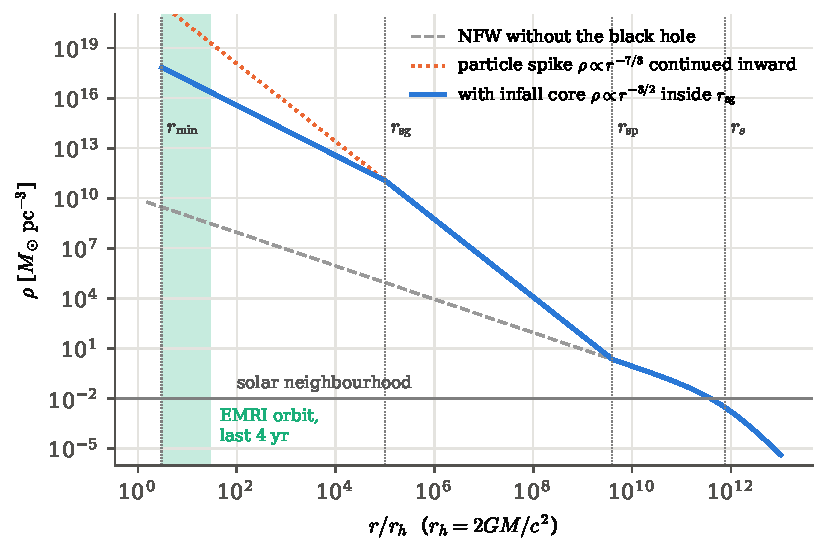
\includegraphics[width=0.82\linewidth]{figures/chT2/dm_profile.pdf}
\caption{Dark matter around a $10^4\,M_\odot$ black hole in a $10^8\,M_\odot$ NFW halo. Without the hole the density would follow the grey dashed NFW profile. Slow growth of the hole turns the cusp inside $r_{\rm sp}$ into a $r^{-7/3}$ spike (dotted where continued inward). Inside the self-gravity radius $r_{\rm sg}=10^5r_h$ an ultralight field falls freely into the hole and the profile flattens to $r^{-3/2}$ (solid). The curves stop at $r_{\rm min}=3r_h$: inside it nothing survives, the hole in the middle of the spike, and the density is zero. The green band is where the EMRI orbits during its last four years; the horizontal line is the density near the Sun.}
\label{T2a:fig:dm-profile}
\end{figure}

\paragraph{Two further wave-dark-matter pictures.}
Kim et al.\ follow the adiabatic compression of a wave halo quantum mechanically \cite{Kim2023}. Far from the hole the compressed wave halo looks like the particle spike, as expected when the wavelength is short. Close to it the picture changes, and the reason is the capture rule used above for particles. A wave component with angular-momentum quantum number $l$ carries angular momentum $l\hbar$, that is $l\hbar/\mu$ per unit mass. A particle with less than $4GM/c$ per unit mass is swallowed, so the components with
\[
  l\lesssim l_{\rm crit}=\frac{4GM}{c}\cdot\frac{\mu}{\hbar}=\frac{2\mu c\,r_h}{\hbar}
\]
fall into the hole, and over the age of the halo they are gone. A component of angular momentum $l$ cannot come closer to the centre than the radius where its centrifugal barrier turns it back, a radius that grows with $l$. Once every component below $l_{\rm crit}$ has been absorbed, nothing is left to fill the region inside the turning radius of $l_{\rm crit}$, and the density is cut off there \cite[eq.~(40)]{Kim2023}. In the particle limit ($\mu r_h c/\hbar\gg1$) $l_{\rm crit}$ is huge and the cutoff is the particle cutoff near $2$--$3r_h$; for light bosons it moves out.

Chase et al.\ consider instead a virialised halo of ultralight \emph{vector} dark matter made of many random waves \cite{Chase2025}. The field oscillates at the frequency $\mu c^2/\hbar$, and its stress, which is quadratic in the field, oscillates at twice that, $\Omega=2\mu c^2/\hbar$. Through Einstein's equations the stress makes the gravitational potential oscillate at $\Omega$ too. What the binary feels depends on the shape of that oscillation. For a scalar the oscillating stress is a pressure, the same in every direction; the oscillating pull on the companion is radial and the same at every point of a circular orbit, so it exerts no torque, and over many field oscillations its effect on the orbit averages to zero. A vector field points along a direction, its polarisation, so its stress is stronger along that axis. The oscillating tidal pull then depends on where the companion is on its orbit: a pattern with two maxima per turn, which exerts a torque proportional to $\sin2(\omega t-\varphi_0)$ for orbital angular frequency $\omega$ and polarisation angle $\varphi_0$, and whose strength oscillates as $\cos\Omega t$. The product
\[
  \cos\Omega t\,\sin2(\omega t-\varphi_0)=\tfrac12\big[\sin\big((2\omega+\Omega)t-2\varphi_0\big)+\sin\big((2\omega-\Omega)t-2\varphi_0\big)\big]
\]
averages to zero over many orbits unless $2\omega\approx\Omega$, when the second term stops oscillating. Away from that condition the pushes cancel; at it they add up, the way a swing responds only to pushes timed to its own period. This is the \newterm{resonance}, and the binary's phase changes mainly while its orbital frequency sweeps through it \cite[Sec.~V]{Chase2025}. The effect is concentrated near one frequency, so, unlike friction and accretion (\cref{T2a:sec:forces}), it cannot be written as a single power of $f$.
\section{Environmental forces and the power law in the phase}
\label{T2a:sec:forces}

Put the light companion of \cref{T2a:sec:chirp} (mass $m_2$, circling the heavy hole $m_1$, with $M=m_1+m_2$) on its orbit inside the spike of \cref{T2a:sec:dm}. It moves at $v=\sqrt{GM/r}$, about $0.13c$ at $30r_h$, through dark matter of density $\rho(r)$. Three things happen. Its gravity focuses the dark matter it passes into a trailing wake, and the wake pulls it back: \newterm{dynamical friction}. It swallows the dark matter that comes close enough, and the swallowed matter has to be brought up to the companion's speed: \newterm{accretion}. And the dark matter inside the orbit adds to the central pull. The first two drain orbital energy on top of the gravitational waves, so the binary sweeps through frequency faster than in vacuum.

The question for the statistics is narrow: \emph{for each effect, by how much does it speed up the sweep at frequency $f$, and what does that do to the Fourier phase $\Psi(f)$?} ($\Psi$ is the phase of the stationary-phase signal of \cref{T2a:sec:spa}, $\tilde h=\mathcal Af^{-7/6}e^{-i\Psi}$.) The answer turns out to have the same form for all of them, a power of $f$ added to the phase, and that is what makes a single, general forecast possible in \cref{ch:10}.

\subsection{The forces}

\paragraph{Dynamical friction.}
For a body of mass $m_2$ moving at speed $v$ through collisionless matter of density $\rho$, Chandrasekhar's formula gives a drag
\begin{equation}
  F_{\rm DF}=\frac{4\pi G^2m_2^2\,\rho\,\xi\ln\Lambda}{v^2}
  \label{T2a:eq:df}
\end{equation}
\cite{Chandrasekhar1943}, \cite[eq.~(16)]{Eda2015}, \cite[eq.~(7)]{Coogan2022}. Every factor can be derived from one deflection.

\emph{One particle passing.} Work in the companion's frame, where the dark matter streams past at speed $v$. Take first the simplest stream, every particle moving at exactly $v$. A particle of mass $m_{\rm dm}\ll m_2$ that would miss the companion by the \newterm{impact parameter} $s$ (we write $s$, not the usual $b$, which is reserved for the ppE exponent below) is bent through an angle $\theta$ given by the Kepler hyperbola, $\tan(\theta/2)=Gm_2/(sv^2)$. Its speed far away is unchanged, only its direction turns, so it loses forward momentum $m_{\rm dm}v(1-\cos\theta)$. That momentum goes to the companion and points along the stream, that is, against the companion's motion through the dark matter. The sideways kicks cancel between particles passing on opposite sides.

\emph{All the particles.} Particles with impact parameter between $s$ and $s+\dd s$ arrive at the rate $(\rho/m_{\rm dm})\,v\,2\pi s\,\dd s$. With $s_{90}\equiv Gm_2/v^2$, the impact parameter that turns a particle through $90^\circ$,
\begin{align}
  F
  &\eqby{1}\int\frac{\rho}{m_{\rm dm}}\,v\,2\pi s\,\dd s\;m_{\rm dm}v\,(1-\cos\theta)
  \eqby{2}4\pi\rho v^2s_{90}^2\int_0^{s_{\max}}\frac{s\,\dd s}{s^2+s_{90}^2}\nonumber\\
  &\eqby{3}\frac{4\pi G^2m_2^2\rho}{v^2}\cdot\frac12\ln\Big(1+\frac{s_{\max}^2}{s_{90}^2}\Big)
  \eqby{4}\frac{4\pi G^2m_2^2\rho}{v^2}\,\ln\Lambda,\qquad\Lambda\equiv\frac{s_{\max}}{s_{90}} .\label{T2a:eq:df-derive}
\end{align}
\begin{explain}
  \item Momentum per particle times the rate of particles, summed over impact parameters. The mass $m_{\rm dm}$ cancels: only the density matters.
  \item $1-\cos\theta=2\sin^2(\theta/2)=2\tan^2(\theta/2)/[1+\tan^2(\theta/2)]=2s_{90}^2/(s^2+s_{90}^2)$, using $\tan(\theta/2)=s_{90}/s$.
  \item $\int s\,\dd s/(s^2+s_{90}^2)=\tfrac12\ln(s^2+s_{90}^2)$; and $v^2s_{90}^2=G^2m_2^2/v^2$.
  \item For $s_{\max}\gg s_{90}$, $\tfrac12\ln(1+\Lambda^2)\approx\ln\Lambda$.
\end{explain}
So each factor has a reason. One $m_2$ comes from the strength of each deflection and the other from the size $s_{90}$ of the region where deflections are strong; the $1/v^2$ says a slow body has more time to bend each particle. The logarithm counts the e-folds of impact parameter between $s_{90}$ and $s_{\max}$, each adding the same amount, so distant encounters matter as much as close ones and the integral must be cut off by hand. The lower end is $s_{\min}=s_{90}$, below which particles are turned right round and nothing more is gained; the upper end $s_{\max}$ is the size of the region in which the stream is a uniform flow, the orbit itself, $s_{\max}\sim r$.

\emph{Particles of all speeds.} A real spike has particles with a spread of speeds. Chandrasekhar showed that for an isotropic distribution the particles faster than the body pull it, on average, equally forwards and backwards, and only those slower than $v$ contribute. The factor $\xi$ in \eqref{T2a:eq:df} is that fraction, $\xi=4\pi\int_0^vf(u)u^2\,\dd u$ for the distribution $f(u)$ of particle speeds. For the $7/3$ spike, whose speeds are set by the hole's potential, it is about $0.58$ \cite{Coogan2022}; papers that ignore the spread set it to one.

\emph{The size of the logarithm.} On a circular orbit $v^2=GM/r$, so $s_{90}=Gm_2/v^2=r\,m_2/M$. With $s_{\max}=r$, $\Lambda\approx M/m_2\approx m_1/m_2$. Coogan et al.\ take a more cautious $s_{\max}=\sqrt{rs_{90}}$, the geometric mean of the two ends, which halves the logarithm: $\ln\Lambda=\ln\sqrt{m_1/m_2}$ \cite{Coogan2022}. For the $10^3+1.4\,M_\odot$ IMRI that is $\TwlnLambdaC$ against $6.6$; others take about $3$ \cite{Eda2015}. Only the logarithm enters, so this factor of two is the size of the uncertainty in the prescription. \emph{Check at $30r_h$.} There $v^2/c^2=r_h/(2r)=1/60$, so $s_{90}=Gm_2/v^2=\tfrac12(2Gm_2/c^2)(c/v)^2=30$ Schwarzschild radii of the companion: the deflections that build the logarithm happen well outside the companion's own horizon, where the Newtonian hyperbola is a fair description. The power the friction removes is $P_{\rm DF}=F_{\rm DF}\,v$.

\paragraph{Friction on a wave.}
If the dark matter is a wave (\cref{T2a:sec:dm}), a wake smaller than its wavelength cannot form. The force keeps the form of \eqref{T2a:eq:df}, with $\xi\ln\Lambda$ replaced by a function of $kr$, where $k=\mu v/\hbar$ is the dark matter's wavenumber \cite[eq.~(D14)]{HuiOstriker2017}, \cite[eq.~(42)]{Kim2023}:
\begin{equation}
  F_{\rm DF}^{\rm wave}=\frac{4\pi G^2m_2^2\rho\,C_w(kr)}{v^2},\qquad
  C_w(kr)=\mathrm{Cin}(2kr)-1+\frac{\sin2kr}{2kr},\qquad \mathrm{Cin}(z)=\int_0^z\frac{1-\cos t}{t}\,\dd t .
  \label{T2a:eq:df-wave}
\end{equation}
Hui and Ostriker obtain it by solving the scattering of the wave by the companion and summing the momentum carried off by its partial waves. The integral shows why it is a softened Coulomb logarithm. Its variable $t$ measures distance in units of the reduced wavelength. Far beyond a wavelength, $\cos t$ oscillates and averages away, and the integrand is $1/t$, the integrand $\dd s/s$ of $\ln\Lambda$. Within a wavelength the interference of the wave ($1-\cos t\approx t^2/2$) kills the integrand. So Cin is a Coulomb logarithm whose lower cutoff is the wavelength instead of $s_{90}$, and whose upper cutoff is the orbit, $z=2kr$; the terms $-1+\sin z/z$ come from the finite size of the region.

Its two limits tell the story. For a short wavelength, $kr\gg1$, split off the logarithm: $\mathrm{Cin}(z)=\gamma_E+\ln z-\mathrm{Ci}(z)$, where $\gamma_E=0.577$ is Euler's constant and $\mathrm{Ci}(z)=-\int_z^\infty\cos t\,\dd t/t$ is a decaying oscillation, of size $\lvert\sin z\rvert/z$ for large $z$. Both $\mathrm{Ci}(z)$ and $\sin z/z$ go to zero, so $C_w\to\ln(2kr)+\gamma_E-1$: a Coulomb logarithm with $s_{\max}\sim r$ and $s_{\min}\sim1/k$, the particle result. For a long wavelength, $z=2kr\ll1$,
\begin{align*}
  C_w
  &\eqby{1}\Big(\frac{z^2}{4}-\frac{z^4}{96}\Big)-1+\Big(1-\frac{z^2}{6}+\frac{z^4}{120}\Big)+O(z^6)
  \eqby{2}\frac{z^2}{12}+O(z^4)=\frac{(kr)^2}{3}+O\big((kr)^4\big),
\end{align*}
\begin{explain}
  \item Expand $1-\cos t=t^2/2-t^4/24$, so $\mathrm{Cin}(z)=z^2/4-z^4/96$; and $\sin z/z=1-z^2/6+z^4/120$.
  \item The constants cancel and $\tfrac14-\tfrac16=\tfrac1{12}$; with $z=2kr$, $z^2/12=(kr)^2/3$.
\end{explain}
so friction is suppressed as $(kr)^2$ when the wavelength exceeds the orbit. \Cref{T2a:fig:wave-df} shows both limits; at $kr=0.1$ the small-$kr$ form is already accurate to $\TwCwSmallErr\%$. This suppression, together with the lower density near the hole, is why wave-like dark matter dephases the inspiral less than particle dark matter of the same mass density \cite[Sec.~III D]{Kim2023}.

\begin{figure}[htbp]
\centering
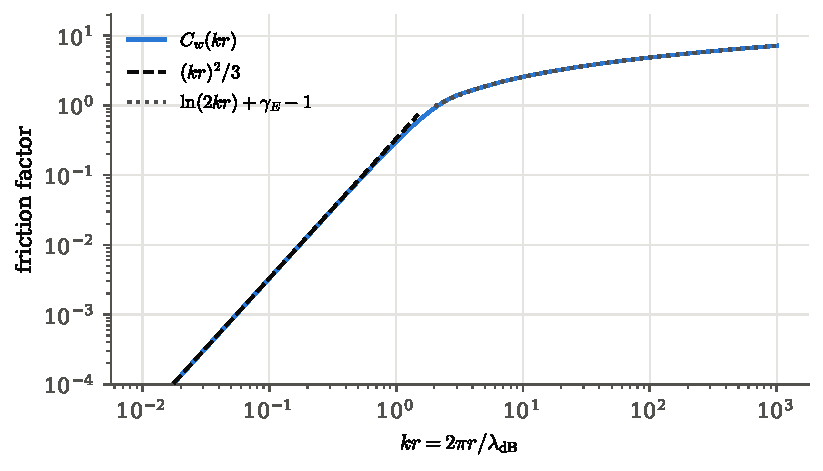
\includegraphics[width=0.75\linewidth]{figures/chT2/wave_df.pdf}
\caption{The friction factor of a wave-like medium as a function of $kr=2\pi r/\lambda_{\rm dB}$. When the de Broglie wavelength is longer than the orbit ($kr\ll1$) friction is suppressed as $(kr)^2/3$ (dashed); when it is shorter, the factor grows like the Coulomb logarithm of particle dark matter (dotted).}
\label{T2a:fig:wave-df}
\end{figure}

\paragraph{Accretion.}
How much dark matter does the companion swallow? In its own rest frame the dark matter streams in at speed $v$, each particle with angular momentum per unit mass $L=sv$ about the companion. General relativity supplies one fact: a particle arriving from far away with $L$ below $L_{\rm crit}=4Gm_2/c$ meets no centrifugal barrier and crosses the horizon (the same capture rule that cuts off the spike near the central hole, \cref{T2a:sec:dm}). Setting $sv=L_{\rm crit}$ gives the capture radius and the cross-section,
\[
  s_{\rm cap}=\frac{4Gm_2}{cv},\qquad \sigma=\pi s_{\rm cap}^2=\frac{16\pi G^2m_2^2}{c^2v^2}.
\]
The mass swallowed per unit time is the mass flux through that area, $\dot m=\rho v\sigma=16\pi G^2m_2^2\rho/(c^2v)$. Now go back to the frame of the spike. There the dark matter is (on average) at rest, and after capture it moves with the companion at speed $v$. The companion must supply that momentum, $\dot m\,v$ per unit time: a drag force $F_{\rm acc}=\dot m\,v$ and a power $P_{\rm acc}=\dot mv^2$. The ratio $s_{\rm cap}/s_{90}=4v/c$ is about $0.5$ at $30r_h$: the particles swallowed are a subset of those strongly deflected, which is why accretion comes out as a correction to friction. Compared with friction,
\begin{equation}
  \frac{P_{\rm acc}}{P_{\rm DF}}
  =\frac{16\pi G^2m_2^2\rho\,v/c^2}{4\pi G^2m_2^2\rho\ln\Lambda/v}
  =\frac{4v^2}{c^2\ln\Lambda}
  =\frac{2r_h}{r\ln\Lambda},
\end{equation}
using $v^2=GM/r=c^2r_h/(2r)$ and $\xi=1$. With $\ln\Lambda=3$ this is $\TwaccRatioThirty$ at $30r_h$ and $\TwaccRatioThree$ at the ISCO. Accretion of collisionless dark matter is a relativistic correction to friction. Kim et al.\ check this for their binaries: over the last five years the companion's mass grows by only about one part in $10^4$ \cite[Sec.~IV A]{Kim2023}. For gas, which is collisional, the Bondi--Hoyle--Lyttleton rate $\dot m\propto\rho/v^3$ applies instead, and accretion then scales exactly like friction \cite[Sec.~X]{Barausse2014}.

\paragraph{The gravitational pull.}
The dark matter inside the orbit adds to the central mass. For the spike $\rho=\rho_6(r_6/r)^\gamma$ (with $\gamma<3$) it weighs
\[
  M_{\rm DM}(<r)=\int_0^r4\pi r'^2\rho_6\Big(\frac{r_6}{r'}\Big)^{\gamma}\dd r'=\frac{4\pi\rho_6r_6^{\gamma}}{3-\gamma}\,r^{3-\gamma}.
\]
By the shell theorem, a spherical mass inside the orbit pulls like a point mass at the centre, so Kepler's law holds with $M_{\rm tot}=M+M_{\rm DM}(<r)$ in place of $M$ \cite[eqs.~(9)--(11)]{Speeney2022}. This removes no energy, but it changes the relation between the frequency and the orbit. How much does it change the chirp? Hold the gravitational-wave frequency $f$ fixed, with $\omega=\pi f$, and treat $M_{\rm DM}$ as a constant addition to the central mass over the small range of radii near the current orbit. Each quantity in the chirp rate is a power of $M_{\rm tot}$:
\begin{align*}
  r&\eqby{1}\Big(\frac{GM_{\rm tot}}{\pi^2f^2}\Big)^{1/3}\propto M_{\rm tot}^{1/3},\qquad
  E\eqby{2}-\frac{GM_{\rm tot}\mu}{2r}=-\frac\mu2(\pi GM_{\rm tot}f)^{2/3}\propto M_{\rm tot}^{2/3},\\
  P_{\rm GW}&\eqby{3}\frac{32}{5}\frac{G}{c^5}\mu^2r^4\omega^6\propto M_{\rm tot}^{4/3},\qquad
  \frac{\dot f}{\dot f_{\rm V}}\eqby{4}\frac{P_{\rm GW}/\lvert\dd E/\dd f\rvert}{(\dots)_{M_{\rm tot}=M}}=\Big(1+\frac{M_{\rm DM}}{M}\Big)^{2/3}\approx1+\frac23\,\frac{M_{\rm DM}(<r)}{M}.
\end{align*}
\begin{explain}
  \item Kepler's law, $\omega^2=GM_{\rm tot}/r^3$.
  \item The binding energy \eqref{T2a:eq:Ef} with $M\to M_{\rm tot}$; $\dd E/\dd f$ scales the same way.
  \item The quadrupole power at fixed $\omega$ depends on $M_{\rm tot}$ only through $r^4$.
  \item The chirp rate of \eqref{T2a:eq:fdot} is $P_{\rm GW}/\lvert\dd E/\dd f\rvert\propto M_{\rm tot}^{4/3-2/3}$; expand for $M_{\rm DM}\ll M$.
\end{explain}
So the pull speeds up the chirp by the fraction
\[
  \epsilon_{\rm pull}=\frac23\,\frac{M_{\rm DM}(<r)}{M}=\frac{8\pi\rho_6r_6^\gamma}{3(3-\gamma)M}\,r^{3-\gamma}\propto f^{-2(3-\gamma)/3},
\]
using $r\propto f^{-2/3}$. The coefficient $\tfrac23$ is leading order only, because $M_{\rm DM}(<r)$ itself changes as the orbit shrinks; the exponent does not depend on that. Friction usually matters more \cite[Sec.~IX]{Barausse2014}.

\subsection{From an extra power to a power law in the phase}

\paragraph{The fractional extra power.}
Throughout, $f$ is the gravitational-wave frequency, twice the orbital one, $f=\omega/\pi$ \eqref{T2g:eq:twice}. Friction drains energy slowly, so at each moment the orbit is still a circle obeying Kepler's law, and its energy at frequency $f$ is the vacuum $E(f)$ of \eqref{T2a:eq:Ef}; only the rate at which it moves through these energies changes. Energy balance now reads $\dd E/\dd t=-(P_{\rm GW}+P_{\rm DF})$, with $P_{\rm GW}$ the quadrupole power of a circular binary \eqref{T2g:eq:power-binary}. As in \eqref{T2a:eq:fdot},
\begin{equation}
  \dot f\eqby{1}-\frac{P_{\rm GW}+P_{\rm DF}}{\dd E/\dd f}
  \eqby{2}\frac{P_{\rm GW}}{\lvert\dd E/\dd f\rvert}\Big(1+\frac{P_{\rm DF}}{P_{\rm GW}}\Big)
  \eqby{3}\dot f_{\rm V}\,\big[1+\epsilon(f)\big],\qquad \epsilon\equiv\frac{P_{\rm DF}}{P_{\rm GW}},
  \label{T2a:eq:fdot-env}
\end{equation}
\begin{explain}
  \item $\dd E/\dd t=(\dd E/\dd f)\,\dot f$, since $E$ depends on time only through $f$.
  \item $\dd E/\dd f<0$; factor out $P_{\rm GW}$.
  \item The first factor is the vacuum rate $\dot f_{\rm V}$ of \eqref{T2a:eq:fdot}.
\end{explain}
This is the energy balance of Kim et al.\ \cite[eq.~(36)]{Kim2023}. For friction in a spike $\rho=\rho_6(r_6/r)^\gamma$ (here and below $\gamma$ is the spike slope $\gamma_{\rm sp}$ of \cref{T2a:sec:dm}, and $\rho_6$ the density at $r_6=10^{-6}$\,pc),
\begin{align}
  \epsilon
  &\eqby{1}\frac{4\pi G^2m_2^2\rho\,\xi\ln\Lambda/v}{\frac{32}{5}G^4M(m_1m_2)^2/(c^5r^5)}
  \eqby{2}\frac{5\pi c^5\xi\ln\Lambda}{8G^{5/2}M^{3/2}m_1^2}\;\rho(r)\,r^{11/2}
  \eqby{3}c_f\,f^{-n},\qquad n=\frac{11-2\gamma}{3}.\label{T2a:eq:eps}
\end{align}
\begin{explain}
  \item $P_{\rm DF}=F_{\rm DF}v$ from \eqref{T2a:eq:df}; $P_{\rm GW}=\tfrac{32}{5}(G/c^5)\mu^2r^4\omega^6=\tfrac{32}{5}G^4M^3\mu^2/(c^5r^5)$ by Kepler, and $M^3\mu^2=M(m_1m_2)^2$ \cite[eq.~(6)]{Coogan2022}.
  \item $m_2^2$ cancels, and $1/v=r^{1/2}(GM)^{-1/2}$. The result $\epsilon\propto\rho r^{11/2}$ is \cite[eq.~(16)]{Speeney2022}.
  \item Insert $\rho=\rho_6r_6^\gamma r^{-\gamma}$, so $\rho r^{11/2}=\rho_6r_6^\gamma\,r^{11/2-\gamma}$, and trade the radius for the gravitational-wave frequency with Kepler's law, $r=(GM/\pi^2f^2)^{1/3}$: $r^{11/2-\gamma}=(GM/\pi^2)^{(11/2-\gamma)/3}f^{-\frac23(\frac{11}2-\gamma)}$, and $\frac23(\frac{11}2-\gamma)=\frac{11-2\gamma}3=n$.
\end{explain}
Collecting the constants of step (3),
\begin{equation}
  c_f=\frac{5\pi c^5\xi\ln\Lambda}{8G^{5/2}M^{3/2}m_1^2}\;\rho_6r_6^{\gamma}\,\Big(\frac{GM}{\pi^2}\Big)^{(11/2-\gamma)/3},
  \label{T2a:eq:cf}
\end{equation}
with units of ${\rm Hz}^n$, so that $c_ff^{-n}$ is a pure number; the $f$ in $c_ff^{-n}$ is the gravitational-wave frequency. Friction and radiation remove energy equally fast where $\epsilon=1$, at $f_{\rm eq}\equiv c_f^{1/n}$.
The same step works for any effect whose power, relative to the gravitational-wave power, varies as a power of the radius: $P_{\rm env}/P_{\rm GW}\propto r^p$ gives $\epsilon\propto f^{-2p/3}$. Since $P_{\rm GW}\propto r^{-5}$ falls so steeply with radius, nearly every environmental effect has $p>0$: it matters most early in the inspiral, at low frequency.

\paragraph{The phase.}
Recall why the chirp rate controls the Fourier phase. The slope of the phase is the arrival time of each frequency, $\dd\Psi/\dd f=2\pi t(f)$, and differentiating once more turns $\dd t/\dd f$ into $1/\dot f$: the curvature of the phase is $2\pi/\dot f$ \eqref{T2a:eq:psi-derivs}, derived with the stationary-phase approximation in \cref{T2a:sec:spa}. A binary that sweeps faster spends less time at each frequency, and the phase bends less. With \eqref{T2a:eq:fdot-env}, and $\dot f_{\rm V}=Kf^{11/3}$, $K=\tfrac{96}{5}\pi^{8/3}(G\mathcal M/c^3)^{5/3}$,
\begin{align}
  \frac{\dd^2\Psi}{\dd f^2}
  &\eqby{1}\frac{2\pi}{\dot f_{\rm V}(1+\epsilon)}
  \eqby{2}\frac{2\pi}{\dot f_{\rm V}}-\frac{2\pi c_f}{K}\,f^{-11/3-n}+O(\epsilon^2),\nonumber\\
  \delta\Psi(f)
  &\eqby{3}-\frac{2\pi c_f}{K\,(n+\frac83)(n+\frac53)}\,f^{-5/3-n}+C_0+C_1f
  \eqby{4}\beta\,u^{\,b},\qquad u\equiv\frac{\pi G\mathcal Mf}{c^3},\quad b=-\frac53-n .\label{T2a:eq:ppe}
\end{align}
\begin{explain}
  \item \eqref{T2a:eq:psi-derivs} with \eqref{T2a:eq:fdot-env}.
  \item $1/(1+\epsilon)=1-\epsilon+\dots$ for $\epsilon\ll1$; the first term gives the vacuum phase \eqref{T2a:eq:psiN}, the second is the change, with $\epsilon/f^{11/3}=c_ff^{-11/3-n}$.
  \item Integrate twice: $f^{-11/3-n}\to f^{-8/3-n}/(-\frac83-n)\to f^{-5/3-n}/[(\frac83+n)(\frac53+n)]$. The two integration constants $C_0+C_1f$ have the form of a shift of $\phi_c$ and of $t_c$ in \eqref{T2a:eq:psiN}, so they are absorbed there (\cref{T2g:sec:tc-phic}).
  \item Rewrite $f=u\,c^3/(\pi G\mathcal M)$, so $f^{-5/3-n}=u^{b}(\pi G\mathcal M/c^3)^{5/3+n}$; all constants go into $\beta$. $u$ is the reduced frequency of \eqref{T2g:eq:u}.
\end{explain}
The amplitude, written out, is
\[
  \beta=-\frac{2\pi c_f}{K\,(n+\frac83)(n+\frac53)}\Big(\frac{\pi G\mathcal M}{c^3}\Big)^{5/3+n}
  =-\frac{5}{48}\,\frac{c_f\,(\pi G\mathcal M/c^3)^{n}}{(n+\frac83)(n+\frac53)},
\]
using $2\pi(\pi G\mathcal M/c^3)^{5/3}/K=\tfrac{10\pi}{96}\pi^{5/3-8/3}=\tfrac5{48}$. It is proportional to $c_f$, hence to the density $\rho_6$ of the spike, and the combination $c_f(\pi G\mathcal M/c^3)^n$ is a pure number. A check: for $n=0$ the environment speeds the chirp up by a constant fraction $c_f$, which by step (2) multiplies the Newtonian term $\tfrac3{128}u^{-5/3}$ of \eqref{T2a:eq:psiN} by $1-c_f$; and indeed $-\tfrac5{48}c_f/(\tfrac83\cdot\tfrac53)=-\tfrac3{128}c_f$.

\begin{keyidea}[Environments are power laws in the phase]
If an environment adds a power $P_{\rm env}$ with $P_{\rm env}/P_{\rm GW}=c_ff^{-n}\ll1$, the Fourier phase gains $\delta\Psi=\beta u^b$ with $u=\pi G\mathcal Mf/c^3$ and $b=-5/3-n$; the amplitude $\beta$ carries the strength of the effect and the exponent $b$ its physics. For dynamical friction in a spike $\rho\propto r^{-\gamma}$, $b=(2\gamma-16)/3$; for $\gamma=7/3$, $b=-34/9\approx-3.78$.
\end{keyidea}

This is the parametrised post-Einsteinian (ppE) phase term $\beta u^b$ of \eqref{T2g:eq:ppe}, now with a definite exponent: the general rule \eqref{T2g:eq:ppe-rule} with $p=-3n$ gives the same $b=-\tfrac53-n$. In the post-Newtonian counting of \cref{T2g:sec:pn}, a correction of relative size $(v/c)^{2k}$ is of order $k$PN, and on a circular orbit $(v/c)^2=(\pi GMf/c^3)^{2/3}\propto f^{2/3}$. So $f^{-n}\propto[(v/c)^2]^{-3n/2}$, and $\epsilon\propto f^{-n}$ is a correction of order $-\tfrac32n$\,PN, so friction in a uniform medium ($\gamma=0$, $n=11/3$) is a $-5.5$PN effect. The dissipative effects, friction and accretion in any spike with $\gamma<3$, have $b<-7/3$: they act more strongly at low frequency than the dipole radiation ($b=-7/3$) and the massive graviton ($b=-1$) of \cref{T2g:sec:pn}. In the Fisher matrix of \cref{ch:10} this is what separates them from the chirp mass, whose own phase term goes as $u^{-5/3}$: two terms with different powers of $f$ are hard to mimic with one another.

\paragraph{The time-domain dephasing.}
Papers on environments usually plot a different phase: the number of radians the wave still has to go through before coalescence. Its phase advances at the rate $2\pi f$, so between frequency $f$ and coalescence at $f_c$
\[
  \Phi(f)=2\pi\int_t^{t_c}f(t')\,\dd t'=2\pi\int_f^{f_c}\frac{f'}{\dot f(f')}\,\dd f',
\]
changing the variable from time to frequency with $\dd t'=\dd f'/\dot f$. The \newterm{dephasing} is the vacuum phase still to come minus the phase still to come in the environment, $\Delta\Phi(f)=\Phi_{\rm V}(f)-\Phi(f)$ \cite[eq.~(49)]{Kim2023}; $\Phi_{\rm V}$ is the $\Phi$ of \cref{T2a:sec:spa} for the Newtonian chirp. A faster sweep leaves fewer cycles, so $\Delta\Phi>0$.

Why two phases? $\Delta\Phi$ is the size that is easy to feel: it counts the radians of wave the environment removes, and once it reaches about a radian a vacuum template is visibly out of step with the signal. The Fisher matrix and the likelihood work in the frequency domain, with the phase $\Psi$ of the template; there part of $\Delta\Phi$ is absorbed by adjusting the arrival time $t_c$ and the phase $\phi_c$, which are fitted anyway. So the two answer different questions, and we compute both.

With \eqref{T2a:eq:fdot-env} and $\dot f_{\rm V}=Kf^{11/3}$,
\begin{align}
  \Delta\Phi(f)
  &\eqby{1}2\pi\int_f^{\infty}\frac{f'}{K f'^{11/3}}\Big(1-\frac1{1+c_ff'^{-n}}\Big)\dd f'
  \eqby{2}\frac{2\pi c_f}{K}\int_f^\infty f'^{-8/3-n}\dd f'\nonumber\\
  &\eqby{3}\frac{2\pi c_f}{K}\,\frac{f^{-5/3-n}}{\frac53+n}
  \eqby{4}\frac{5\,c_f f^{-n}}{2(8-\gamma)}\,\Phi_{\rm V}(f).\label{T2a:eq:dPhi}
\end{align}
\begin{explain}
  \item The difference of the two phase integrals, $1/\dot f_{\rm V}-1/\dot f=\frac1{\dot f_{\rm V}}\big(1-\frac1{1+\epsilon}\big)$, with the upper limit $f_c$ sent to infinity (justified below).
  \item $1-1/(1+\epsilon)\approx\epsilon=c_ff'^{-n}$ for $\epsilon\ll1$.
  \item $\int_f^\infty f'^{-8/3-n}\dd f'=f^{-5/3-n}/(\frac53+n)$.
  \item $\Phi_{\rm V}=\frac{2\pi}{K}\cdot\frac35f^{-5/3}$, so the ratio is $\frac{5}{3}c_ff^{-n}/(\frac53+n)=5c_ff^{-n}/(5+3n)$, and $5+3n=16-2\gamma$.
\end{explain}
\emph{The upper limit.} The integrand of $\Delta\Phi$ falls as $f'^{-8/3-n}$, so the part beyond $f_c$ is a fraction $(f/f_c)^{5/3+n}$ of the whole. For the IMRI, with $f_c$ the ISCO frequency of about $4.4$\,Hz and $f$ the $\TwffourImri$\,mHz at which the four-year window opens, that fraction is about $2\times10^{-9}$ for $\gamma=7/3$, and smaller still for the other slopes. Integrating to infinity, as here, and stopping at the ISCO, as the script does, give the same numbers to that accuracy.

This is the high-frequency limit quoted by Coogan et al.\ \cite[eq.~(16)]{Coogan2022}, and it has the same exponent $-5/3-n$ as $\delta\Psi$. The two coefficients compare in one line: from \eqref{T2a:eq:ppe} and \eqref{T2a:eq:dPhi},
\[
  \frac{\delta\Psi}{\Delta\Phi}
  =\frac{-2\pi c_f/[K(n+\frac83)(n+\frac53)]}{2\pi c_f/[K(n+\frac53)]}
  =-\frac1{n+\frac83}\qquad(f\gg f_{\rm eq}),
\]
and for $n=0$ (a constant fractional speed-up) this is the factor $\tfrac38$ between the two kinds of phase found in \cref{T2a:sec:spa}. The sign only records that $\Delta\Phi$ is defined as vacuum minus environment.

\emph{Without the expansion.} Step (2) needs $\epsilon\ll1$, i.e.\ $f\gg f_{\rm eq}$. The integral can also be done exactly. Write the geometric series $1/(1+\epsilon)=\sum_k(-\epsilon)^k$ and integrate term by term:
\begin{align}
  \Phi(f)
  &\eqby{1}\frac{2\pi}{K}\sum_{k=0}^\infty(-c_f)^k\int_f^\infty f'^{-8/3-kn}\dd f'\nonumber\\
  &\eqby{2}\Phi_{\rm V}(f)\sum_{k=0}^\infty\frac{a}{a+k}\big(-c_ff^{-n}\big)^k\nonumber\\
  &\eqby{3}\Phi_{\rm V}(f)\;{}_2F_1\big(1,a;1+a;-c_ff^{-n}\big),\qquad a\equiv\frac5{3n}.\label{T2a:eq:hyp}
\end{align}
\begin{explain}
  \item $\Phi=2\pi\int_f^\infty f'/\dot f\,\dd f'$ with $\dot f=Kf'^{11/3}(1+c_ff'^{-n})$.
  \item $\int_f^\infty f'^{-8/3-kn}\dd f'=f^{-5/3-kn}/(\tfrac53+kn)$; factoring out the $k=0$ term, which is $\Phi_{\rm V}$, leaves $\tfrac{5/3}{5/3+kn}=\tfrac{a}{a+k}$.
  \item The \newterm{Pochhammer symbol} is the rising product $(x)_k=x(x+1)\cdots(x+k-1)$, with $(x)_0=1$. In $\frac{(a)_k}{(1+a)_k}=\frac{a(a+1)\cdots(a+k-1)}{(a+1)\cdots(a+k)}$ every factor but the first on top and the last below cancels, leaving $\frac{a}{a+k}$. The \newterm{hypergeometric function} is the series ${}_2F_1(\alpha,\beta;\gamma';z)=\sum_k\frac{(\alpha)_k(\beta)_k}{(\gamma')_k\,k!}z^k$; with $\alpha=1$, $(1)_k=k!$ cancels the $k!$, and with $\beta=a$, $\gamma'=1+a$ the series is $\sum_k\frac{a}{a+k}z^k$.
\end{explain}
The geometric series converges only for $\epsilon<1$, yet the phase at lower frequencies, where friction dominates, is a perfectly finite integral. The same substitution that turned the series into ${}_2F_1$ shows that nothing is lost. Put $t=(f/f')^n$ in the exact integral, with $z=-c_ff^{-n}$:
\begin{align*}
  \frac{K}{2\pi}\Phi(f)
  &\eqby{1}\int_f^\infty\frac{f'^{-8/3}\,\dd f'}{1+c_ff'^{-n}}
  \eqby{2}\frac{f^{-5/3}}{n}\int_0^1\frac{t^{a-1}\,\dd t}{1-zt}
  \eqby{3}\frac35f^{-5/3}\;a\!\int_0^1\frac{t^{a-1}\,\dd t}{1-zt}.
\end{align*}
\begin{explain}
  \item The definition with $\dot f=Kf'^{11/3}(1+c_ff'^{-n})$.
  \item $f'=ft^{-1/n}$, $\dd f'=-(f/n)t^{-1/n-1}\dd t$, and $c_ff'^{-n}=c_ff^{-n}t=-zt$; the powers of $t$ combine to $t^{(8/3-1)/n-1}=t^{a-1}$, and $f'$ from $f$ to $\infty$ is $t$ from $1$ to $0$.
  \item $1/n=\tfrac35a$.
\end{explain}
Expanding $1/(1-zt)=\sum_k(zt)^k$ and using $a\int_0^1t^{a-1+k}\dd t=a/(a+k)$ returns exactly the series of \eqref{T2a:eq:hyp}, so the last integral \emph{is} ${}_2F_1(1,a;1+a;z)$ where the series converges. But the integral is finite and smooth for every $z\le0$, since $1-zt\ge1$, so it defines the function at every frequency; this is Euler's integral for the hypergeometric function, the standard way of continuing it beyond $\lvert z\rvert<1$. Hence \eqref{T2a:eq:hyp} holds at all frequencies \cite[eq.~(12)]{Coogan2022}. At low frequency, $f\to0$, $z\to-\infty$ and the integral goes to zero: friction then sweeps the binary through each frequency so fast that it accumulates almost none of the vacuum phase, and $\Delta\Phi\to\Phi_{\rm V}$.

\subsection{The experiment: dephasing for several spike slopes}
\label{T2a:sec:coogan}

\subsubsection*{Their question}
Coogan et al.\ asked whether LISA could tell an intermediate-mass-ratio inspiral wrapped in a dark-matter spike from the same binary in vacuum, and whether the signal would then measure the spike's density and slope \cite{Coogan2022}. Earlier estimates had used a fixed spike and found enormous dephasings. Their point was that the friction heats the spike it feeds on, so the honest question is what survives once the spike is allowed to respond. We reproduce the static part of their calculation, which is what the equations of this section describe, and use it to see where the static picture stops.

\subsubsection*{Their setup}
The binary is a $10^3\,M_\odot$ black hole with a $1.4\,M_\odot$ companion, the IMRI of \cref{T2a:sec:chirp}. Around the heavy hole sits a spike $\rho=\rho_6(r_6/r)^\gamma$ whose density at the pivot radius $r_6=10^{-6}$\,pc is fixed to their benchmark value (\cref{T2a:sec:dm} derived it from $\rho_{\rm sp}=226\,M_\odot\,{\rm pc}^{-3}$). The companion feels Chandrasekhar's friction \eqref{T2a:eq:df}, with the fraction $\xi$ of slow particles appropriate for a $7/3$ spike and their logarithm $\ln\sqrt{m_1/m_2}$. We keep $\rho_6$ fixed and vary the slope, to see how the dephasing depends on $\gamma$, and we look at the last four years before the ISCO, a nominal LISA mission.
\begin{center}
\small
\begin{tabular}{@{}lll@{}}
\toprule
quantity & meaning & value\\\midrule
$m_1$, $m_2$ & central hole, companion & $10^3\,M_\odot$, $1.4\,M_\odot$\\
$\rho_6$ & spike density at $r_6$ & $5.45\times10^{15}\,M_\odot\,{\rm pc}^{-3}$\\
$r_6$ & pivot radius & $10^{-6}$\,pc\\
$\xi$ & fraction of slower particles & $0.58$\\
$\ln\Lambda$ & Coulomb logarithm, $\ln\sqrt{m_1/m_2}$ & $\TwlnLambdaC$\\
$\gamma$ & spike slope & $1.5$, $2$, $7/3$, $2.5$\\
window & last four years before the ISCO & from $\TwffourImri$\,mHz\\
\bottomrule
\end{tabular}
\end{center}

\subsubsection*{Their equations in ours}
Everything needed has been derived above, and we kept their symbols wherever they had one: $\rho_6$, $r_6$, $c_f$ and $f_{\rm eq}$ mean the same here as there, and $f$ is in both cases the gravitational-wave frequency.
\begin{center}
\small
\begin{tabular}{@{}lll@{}}
\toprule
Coogan et al. & here & content\\\midrule
eq.~(12) & \eqref{T2a:eq:hyp} & exact phase to coalescence in a static spike\\
eq.~(15) & $f_{\rm eq}=c_f^{1/n}$, with \eqref{T2a:eq:cf} & where friction and radiation are equal\\
eq.~(16) & \eqref{T2a:eq:dPhi} & high-frequency power law of the dephasing\\
\bottomrule
\end{tabular}
\end{center}
The one convention to watch is which phase is quoted: their dephasing is the time-domain $\Delta\Phi$, not the Fourier $\delta\Psi$ of the Fisher matrix, and the two differ by the factor $-1/(n+\tfrac83)$ derived above.

\subsubsection*{What we compute}
The script \pyname{05_dephasing.py} evaluates these formulas for the four slopes:

\pyfile[firstline=36,lastline=51,firstnumber=36]{code/chT2/05_dephasing.py}{The friction-to-radiation ratio and the exact dephasing}

\noindent It makes four moves. First, lines 38--39 compute the constants of \eqref{T2a:eq:cf}: \pyname{rho_SI} is $\rho_6r_6^\gamma$ in SI units, and \pyname{pref} is the prefactor of step (2) of \eqref{T2a:eq:eps}. Second, line 41 completes $c_f$ by writing the radius through Kepler's law, the factor $(GM/\pi^2)^{(11-2\gamma)/6}$, so that $\epsilon=c_ff^{-n}$ is a function of the frequency alone. Third, lines 45 and 51 evaluate the vacuum phase $\Phi_{\rm V}=\tfrac1{16}(\pi G\mathcal Mf/c^3)^{-5/3}$ and the exact dephasing $\Phi_{\rm V}(1-{}_2F_1)$ of \eqref{T2a:eq:hyp}; the variable \pyname{b} on line 50 is the parameter $a=5/(3n)$, and \pyname{dphi_closed} is $\Delta\Phi$. Fourth, the script integrates $2\pi f/\dot f$ directly, with no expansion and no hypergeometric function, and compares: the two agree to $\TwclosedVsNum$. That check tests the algebra from $\epsilon$ to $\Phi$, the series, the substitution and the code; it says nothing about whether the static-spike physics is right. The dephasing plotted is accumulated between $f$ and the ISCO, as in \cite[eq.~(49)]{Kim2023}.

\begin{figure}[htbp]
\centering
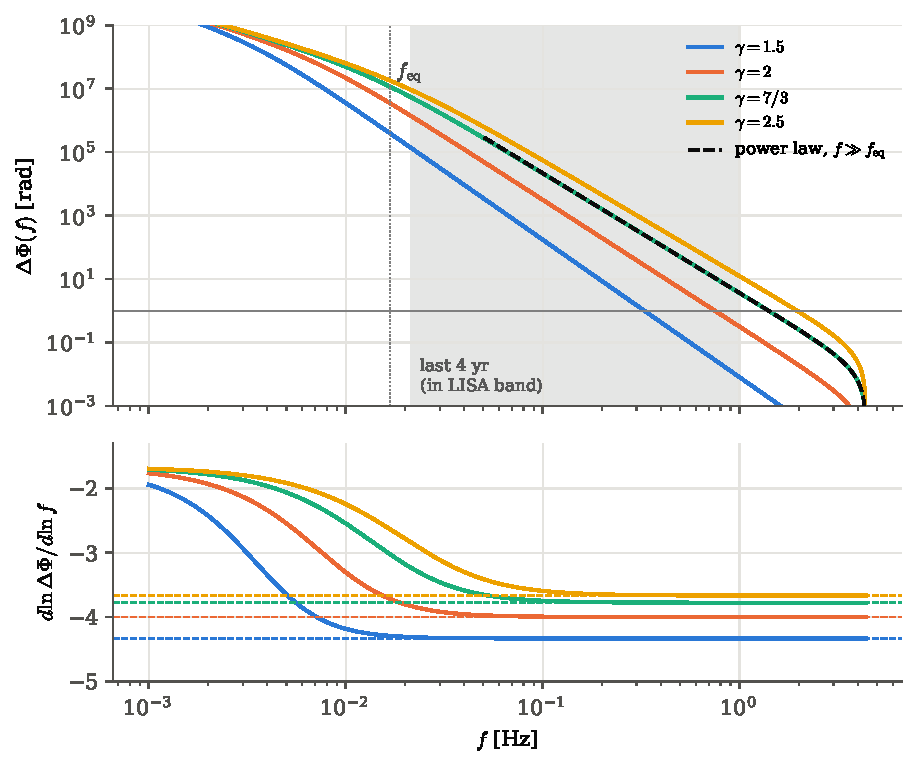
\includegraphics[width=0.85\linewidth]{figures/chT2/dephasing.pdf}
\caption{Dephasing of the $10^3+1.4\,M_\odot$ IMRI by friction in a static spike of slope $\gamma$, at fixed density $\rho_6$ at $10^{-6}$\,pc. Top: phase lost between $f$ and the ISCO; the dashed black line is the power law \eqref{T2a:eq:dPhi} for $\gamma=7/3$, drawn where $f>3f_{\rm eq}$, and the grey band is the last four years. Bottom: the local slope $\dd\ln\Delta\Phi/\dd\ln f$ of the phase lost before coalescence. It moves from the vacuum value $-5/3$ at low frequency to the predicted $-5/3-n$ (dashed, one per slope) above $f_{\rm eq}$.}
\label{T2a:fig:dephasing}
\end{figure}

\subsubsection*{Reading the figure}
\Cref{T2a:fig:dephasing} has one idea: the dephasing is a broken power law, with the break at $f_{\rm eq}$. For $\gamma=7/3$ friction and radiation balance at $f_{\rm eq}=\TwfeqC$\,mHz. Below $f_{\rm eq}$ friction drives the inspiral, almost all of the vacuum phase is lost ($\Delta\Phi\to\Phi_{\rm V}$, as found above), and the local slope of $\Delta\Phi$ is the vacuum $-5/3$. Above it each curve settles onto the predicted exponent $b=-5/3-n$ of \eqref{T2a:eq:dPhi}: the measured local slopes are $\TwbexpA$, $\TwbexpB$, $\TwbexpC$ and $\TwbexpD$ for $\gamma=1.5$, $2$, $7/3$, $2.5$, against $-13/3$, $-4$, $-34/9$ and $-11/3$.

\subsubsection*{How large}
The steeper the spike, the more phase it removes at fixed $\rho_6$: over the last four years before the ISCO (from $\TwffourImri$\,mHz), $\Delta\Phi=\TwdPhiFourA$, $\TwdPhiFourB$, $\TwdPhiFourC$ and $\TwdPhiFourD$\,rad for the four slopes. To give these a scale: a matched filter at signal-to-noise ratio $\rho$ resolves a phase error of about $1/\rho$ radians, the weighted root-mean-square phase shift that the Fisher matrix can detect (\cref{10b:sec:fisher-structure}), about a tenth of a radian for $\rho=10$. So even the gentlest of these spikes would be glaringly visible in this idealised, static setting.

\subsubsection*{Paper and reproduction side by side}
\begin{center}
\small
\begin{tabularx}{\linewidth}{@{}>{\raggedright\arraybackslash}p{0.24\linewidth} >{\raggedright\arraybackslash}X >{\raggedright\arraybackslash}X@{}}
\toprule
quantity ($\gamma=7/3$) & Coogan et al. & ours (static)\\\midrule
$f_{\rm eq}$ & $\approx15$\,mHz \cite[eq.~(15)]{Coogan2022} & $\TwfeqC$\,mHz\\
high-frequency slope of $\Delta\Phi$ & $-34/9$ (static, eq.~(16)) & $\TwbexpC$\\
exact vs.\ power law & eq.~(12) & closed form = numerical to $\TwclosedVsNum$\\
$\Delta\Phi$, last four years & much smaller, spike with feedback (Sec.~IV) & $\TwdPhiFourC$\,rad\\
\bottomrule
\end{tabularx}
\end{center}

\subsubsection*{Why they differ}
\emph{The equality frequency.} Ours is $12\%$ above theirs. Since $f_{\rm eq}=c_f^{1/n}$ and $c_f\propto\xi\ln\Lambda\,\rho_6$, $f_{\rm eq}\propto(\xi\ln\Lambda\,\rho_6)^{1/n}=(\xi\ln\Lambda\,\rho_6)^{9/19}$ for $\gamma=7/3$. A $12\%$ shift in $f_{\rm eq}$ therefore corresponds to a $(1.12)^{19/9}-1\approx26\%$ difference in the product $\xi\ln\Lambda\,\rho_6$. The prescriptions differ by more than that: setting $\xi=1$ instead of $0.58$ alone would move $f_{\rm eq}$ up by $(1/0.58)^{9/19}\approx1.29$, and the two common choices of $\ln\Lambda$ differ by a factor of two. We have not pinned the remaining $12\%$ on a single choice; it is the size expected from these conventions, and the exponents, which do not depend on them, agree.

\emph{Static against responding spike.} This is the large difference. The energy friction removes from the orbit goes into the dark matter, and a rough count shows it is far more than the spike can absorb. Take the orbit at $f_{\rm eq}$, of radius $r=(GM/\pi^2f_{\rm eq}^2)^{1/3}\approx1.2\times10^{-8}$\,pc. The energy friction removes between $f_{\rm eq}$ and the ISCO is the friction share of the orbital energy lost,
\[
  E_{\rm DF}=\int_{f_{\rm eq}}^{f_c}\frac{\epsilon}{1+\epsilon}\Big\lvert\frac{\dd E}{\dd f}\Big\rvert\dd f
  =\frac\mu3\Big(\frac{\pi GMf_{\rm eq}}{c^3}\Big)^{2/3}c^2\int_1^{f_c/f_{\rm eq}}\frac{y^{-1/3}\,\dd y}{1+y^{n}}
  \approx1\times10^{-3}\,M_\odot c^2,
\]
with $y=f/f_{\rm eq}$, $\epsilon=y^{-n}$, $\lvert\dd E/\dd f\rvert$ from \eqref{T2a:eq:Ef}, and the last integral $\approx0.51$. The dark matter inside that orbit is $M_{\rm DM}(<r)=4\pi\rho_6r_6^\gamma r^{3-\gamma}/(3-\gamma)\approx5\times10^{-3}\,M_\odot$, bound to the hole by roughly $GMM_{\rm DM}/r\approx2\times10^{-5}\,M_\odot c^2$. The friction deposits some fifty times the binding energy of the dark matter it moves through. The spike near the orbit cannot stay as it was: it is heated and partly unbound, its density at a given radius falls during the inspiral, $\epsilon$ at fixed $f$ falls with it, and the dephasing is smaller and its break moves. That is the qualitative result Coogan et al.\ find when they follow this feedback: a much smaller dephasing, still a broken power law, but with a different break frequency and exponents \cite[Sec.~IV]{Coogan2022}. Kim et al.\ mimic the same effect by capping the friction at the binding energy of a shell of halo \cite[Sec.~IV C]{Kim2023}.

\emph{The chirp itself.} Our vacuum chirp is Newtonian and circular. Near the ISCO, where $v\approx0.4c$, post-Newtonian corrections to $\dot f$ are large (\cref{T2g:sec:pn}), and relativistic corrections to the spike and to the friction push the other way from feedback, increasing the dephasing \cite{Speeney2022}. These change the numbers, not the exponents of \eqref{T2a:eq:ppe}, which survive as the leading-order description of each effect.

\subsubsection*{What it taught us}
The power law is not the whole story even before feedback. LISA's window is not far above $f_{\rm eq}$: at the start of the four-year window the power law misses the exact $\Delta\Phi$ for $\gamma=7/3$ by $\TwPLerrFour\%$, and for $\gamma=2.5$ the window starts \emph{below} $f_{\rm eq}=\TwfeqD$\,mHz, where no expansion in $\epsilon$ holds. A ppE forecast is reliable when the observed band lies well above $f_{\rm eq}$, that is, for weak environments, which are exactly the ones whose detectability is in question; and a static spike strong enough to matter is one that the binary itself would destroy.

\begin{taxonomy}[Environmental effects as power laws in the phase]
\small
\renewcommand{\arraystretch}{1.25}
\begin{tabularx}{\linewidth}{@{}>{\raggedright\arraybackslash}X >{\centering\arraybackslash}p{2.0cm} >{\centering\arraybackslash}p{1.9cm} >{\centering\arraybackslash}p{2.1cm} >{\centering\arraybackslash}p{1.5cm}@{}}
\toprule
effect & $P_{\rm env}/P_{\rm GW}\propto$ & $n$ & $b=-\frac53-n$ & at $\gamma=\frac73$\\\midrule
friction, spike $\rho\propto r^{-\gamma}$ & $r^{11/2-\gamma}$ & $\frac{11-2\gamma}{3}$ & $\frac{2\gamma-16}{3}$ & $-\frac{34}{9}$\\
friction, uniform density & $r^{11/2}$ & $\frac{11}{3}$ & $-\frac{16}{3}$ ($-5.5$PN) & ---\\
accretion, collisionless & $r^{9/2-\gamma}$ & $\frac{9-2\gamma}{3}$ & $\frac{2\gamma-14}{3}$ & $-\frac{28}{9}$\\
accretion, gas (BHL) & as friction & & & \\
pull of enclosed mass (no loss) & $r^{3-\gamma}$ (relative) & $\frac{2(3-\gamma)}{3}$ & $\frac{2\gamma-11}{3}$ & $-\frac{19}{9}$\\
dipole radiation (Brans--Dicke) & $r$ & $\frac23$ & $-\frac73$ & ---\\
vector ultralight DM & \multicolumn{4}{l}{resonant: a step near one frequency, not a power law \cite{Chase2025}}\\
\bottomrule
\end{tabularx}
\end{taxonomy}

The table also marks where the power-law picture stops. The oscillating potential of a vector dark-matter halo (\cref{T2a:sec:dm}) does nothing on average until the orbital frequency crosses a resonance with the field, and then shifts the phase within a narrow band \cite[Sec.~V]{Chase2025}. A template $\beta u^b$ cannot represent such a step; it needs its own model. The ppE parametrisation is a statement about smooth, monotonic effects, and its hidden assumption is that the environment changes slowly with radius.

\paragraph{Where each item is used.}
The waveform \eqref{T2a:eq:hf} with phase \eqref{T2a:eq:psiN} and the correction \eqref{T2a:eq:ppe}, together with the noise \eqref{T2a:eq:Sn}, are the inputs of the gravitational-wave Fisher forecast in \cref{ch:10}, which computes the error on $\beta$ for a list of exponents $b$ and checks it with the sampler of \cref{ch:09}. The density profiles and the parametrisation by $\rho_6$ fix the physical meaning of $\beta$ there. The likelihood $-\tfrac12(d-h\,|\,d-h)$ with this $S_n$ is the one derived in \cref{ch:00}, and comparing a vacuum template with a dressed one is a Bayesian model comparison of the kind treated in \cref{ch:05}.

\begin{recap}
\begin{itemize}[itemsep=1pt]
  \item Energy balance with the quadrupole formula gives the chirp $\dot f=\frac{96}{5}\pi^{8/3}(G\mathcal M/c^3)^{5/3}f^{11/3}$; only the chirp mass enters at leading order, and LISA's benchmark inspirals complete millions of cycles in four years.
  \item The stationary-phase approximation gives $\tilde h=\mathcal Af^{-7/6}e^{-i\Psi(f)}$ with $\dd^2\Psi/\dd f^2=2\pi/\dot f$: anything that changes the sweep rate changes the phase.
  \item LISA's sensitivity $S_n(f)$ combines test-mass acceleration noise (low $f$), optical metrology noise and the arm response (high $f$), and the Galactic confusion foreground (around a millihertz); the signal-to-noise ratio is $\int(h_c/h_n)^2\dd\ln f$.
  \item Slow growth of a black hole compresses a cusp $r^{-\gamma_i}$ into a spike $r^{-(9-2\gamma_i)/(4-\gamma_i)}$, $r^{-7/3}$ for NFW, raising the density at the orbit by some eighteen orders of magnitude; ultralight dark matter falls freely inside the self-gravity radius, $\rho\propto r^{-3/2}$.
  \item An extra power $P_{\rm env}=c_ff^{-n}P_{\rm GW}$ shifts the phase by $\beta u^{b}$, $b=-5/3-n$, valid for $f\gg f_{\rm eq}$; resonant effects are not power laws.
\end{itemize}
\end{recap}

\providecommand{\TwbN}{}\renewcommand{\TwbN}{400}
\providecommand{\TwbAlpha}{}\renewcommand{\TwbAlpha}{0.15}
\providecommand{\TwbBeta}{}\renewcommand{\TwbBeta}{3}
\providecommand{\TwbSigInt}{}\renewcommand{\TwbSigInt}{0.1}
\providecommand{\TwbSigC}{}\renewcommand{\TwbSigC}{0.1}
\providecommand{\TwbErrC}{}\renewcommand{\TwbErrC}{0.03}
\providecommand{\TwbSigXone}{}\renewcommand{\TwbSigXone}{1}
\providecommand{\TwbErrXone}{}\renewcommand{\TwbErrXone}{0.15}
\providecommand{\TwbRawSd}{}\renewcommand{\TwbRawSd}{0.344}
\providecommand{\TwbRawPred}{}\renewcommand{\TwbRawPred}{0.353}
\providecommand{\TwbStdSd}{}\renewcommand{\TwbStdSd}{0.142}
\providecommand{\TwbStdPred}{}\renewcommand{\TwbStdPred}{0.140}
\providecommand{\TwbAhat}{}\renewcommand{\TwbAhat}{0.146}
\providecommand{\TwbBhat}{}\renewcommand{\TwbBhat}{2.67}
\providecommand{\TwbMhat}{}\renewcommand{\TwbMhat}{-19.262}
\providecommand{\TwbNmock}{}\renewcommand{\TwbNmock}{2000}
\providecommand{\TwbBmean}{}\renewcommand{\TwbBmean}{2.754}
\providecommand{\TwbBsd}{}\renewcommand{\TwbBsd}{0.071}
\providecommand{\TwbAmean}{}\renewcommand{\TwbAmean}{0.1467}
\providecommand{\TwbAmeanErr}{}\renewcommand{\TwbAmeanErr}{0.0002}
\providecommand{\TwbLamC}{}\renewcommand{\TwbLamC}{0.917}
\providecommand{\TwbBpred}{}\renewcommand{\TwbBpred}{2.752}
\providecommand{\TwbLamX}{}\renewcommand{\TwbLamX}{0.978}
\providecommand{\TwbApred}{}\renewcommand{\TwbApred}{0.1467}
\providecommand{\TwbPvMag}{}\renewcommand{\TwbPvMag}{0.030}
\providecommand{\TwlNanc}{}\renewcommand{\TwlNanc}{3}
\providecommand{\TwlSigGeo}{}\renewcommand{\TwlSigGeo}{0.03}
\providecommand{\TwlNcephAnc}{}\renewcommand{\TwlNcephAnc}{100}
\providecommand{\TwlNcephCal}{}\renewcommand{\TwlNcephCal}{30}
\providecommand{\TwlSigCeph}{}\renewcommand{\TwlSigCeph}{0.25}
\providecommand{\TwlNcal}{}\renewcommand{\TwlNcal}{40}
\providecommand{\TwlSigSn}{}\renewcommand{\TwlSigSn}{0.13}
\providecommand{\TwlNhf}{}\renewcommand{\TwlNhf}{280}
\providecommand{\TwlSigHf}{}\renewcommand{\TwlSigHf}{0.14}
\providecommand{\TwlHtrue}{}\renewcommand{\TwlHtrue}{73}
\providecommand{\TwlHhat}{}\renewcommand{\TwlHhat}{73.90}
\providecommand{\TwlHerr}{}\renewcommand{\TwlHerr}{1.10}
\providecommand{\TwlFrac}{}\renewcommand{\TwlFrac}{1.49}
\providecommand{\TwlFracApprox}{}\renewcommand{\TwlFracApprox}{1.49}
\providecommand{\TwlNpar}{}\renewcommand{\TwlNpar}{47}
\providecommand{\TwlCanc}{}\renewcommand{\TwlCanc}{0.80}
\providecommand{\TwlCceph}{}\renewcommand{\TwlCceph}{0.74}
\providecommand{\TwlCsn}{}\renewcommand{\TwlCsn}{0.95}
\providecommand{\TwlChf}{}\renewcommand{\TwlChf}{0.38}
\providecommand{\TwlFracFive}{}\renewcommand{\TwlFracFive}{3.05}
\providecommand{\TwlFracOneSixty}{}\renewcommand{\TwlFracOneSixty}{1.22}
\providecommand{\TwlNmc}{}\renewcommand{\TwlNmc}{400}
\providecommand{\TwlMcMean}{}\renewcommand{\TwlMcMean}{72.99}
\providecommand{\TwlMcSd}{}\renewcommand{\TwlMcSd}{1.10}
\providecommand{\TwlMcErr}{}\renewcommand{\TwlMcErr}{1.09}
\providecommand{\TwlCover}{}\renewcommand{\TwlCover}{70\%}
\providecommand{\TwmSigThree}{}\renewcommand{\TwmSigThree}{-0.1280}
\providecommand{\TwmSigThreeTh}{}\renewcommand{\TwmSigThreeTh}{-0.1243}
\providecommand{\TwmSigOne}{}\renewcommand{\TwmSigOne}{-0.0138}
\providecommand{\TwmSigOneTh}{}\renewcommand{\TwmSigOneTh}{-0.0138}
\providecommand{\TwmSigFive}{}\renewcommand{\TwmSigFive}{-0.348}
\providecommand{\TwmSigFiveTh}{}\renewcommand{\TwmSigFiveTh}{-0.345}
\providecommand{\TwmLim}{}\renewcommand{\TwmLim}{24}
\providecommand{\TwmSig}{}\renewcommand{\TwmSig}{0.15}
\providecommand{\TwmNmock}{}\renewcommand{\TwmNmock}{200}
\providecommand{\TwmOm}{}\renewcommand{\TwmOm}{0.3}
\providecommand{\TwmNaiveMean}{}\renewcommand{\TwmNaiveMean}{0.353}
\providecommand{\TwmNaiveSd}{}\renewcommand{\TwmNaiveSd}{0.019}
\providecommand{\TwmCorrMean}{}\renewcommand{\TwmCorrMean}{0.301}
\providecommand{\TwmCorrSd}{}\renewcommand{\TwmCorrSd}{0.018}
\providecommand{\TwmZhalf}{}\renewcommand{\TwmZhalf}{0.73}
\providecommand{\TwmResLast}{}\renewcommand{\TwmResLast}{-0.140}
\providecommand{\TwmResLastTh}{}\renewcommand{\TwmResLastTh}{-0.175}
\providecommand{\TwmNkept}{}\renewcommand{\TwmNkept}{3608}
\providecommand{\TwmZlast}{}\renewcommand{\TwmZlast}{0.75}
\providecommand{\TwtL}{}\renewcommand{\TwtL}{1000}
\providecommand{\TwtN}{}\renewcommand{\TwtN}{128}
\providecommand{\TwtR}{}\renewcommand{\TwtR}{10}
\providecommand{\TwtSigR}{}\renewcommand{\TwtSigR}{0.229}
\providecommand{\TwtKmax}{}\renewcommand{\TwtKmax}{0.05}
\providecommand{\TwtNuTwo}{}\renewcommand{\TwtNuTwo}{2}
\providecommand{\TwtBLthTwo}{}\renewcommand{\TwtBLthTwo}{1.57}
\providecommand{\TwtBLmTwo}{}\renewcommand{\TwtBLmTwo}{1.71}
\providecommand{\TwtBEthTwo}{}\renewcommand{\TwtBEthTwo}{2.57}
\providecommand{\TwtBEmTwo}{}\renewcommand{\TwtBEmTwo}{2.62}
\providecommand{\TwtBLthOne}{}\renewcommand{\TwtBLthOne}{1.01}
\providecommand{\TwtBLmOne}{}\renewcommand{\TwtBLmOne}{1.06}
\providecommand{\TwtBLerrOne}{}\renewcommand{\TwtBLerrOne}{0.03}
\providecommand{\TwtNuHighTwo}{}\renewcommand{\TwtNuHighTwo}{1.32}
\providecommand{\TwtNuHighLast}{}\renewcommand{\TwtNuHighLast}{1.65}
\providecommand{\TwtNbar}{}\renewcommand{\TwtNbar}{3\times10^{-4}}
\providecommand{\TwtNgal}{}\renewcommand{\TwtNgal}{299091}
\providecommand{\TwtShot}{}\renewcommand{\TwtShot}{3343}
\providecommand{\TwtBG}{}\renewcommand{\TwtBG}{2.24}
\providecommand{\TwtBGerr}{}\renewcommand{\TwtBGerr}{0.06}
\providecommand{\TwtBGauto}{}\renewcommand{\TwtBGauto}{2.19}
\providecommand{\TwtBGautoNaive}{}\renewcommand{\TwtBGautoNaive}{2.42}
\providecommand{\TwtOneHalo}{}\renewcommand{\TwtOneHalo}{7114}
\providecommand{\TwtLam}{}\renewcommand{\TwtLam}{2.13}
\providecommand{\TwtRatioParNaive}{}\renewcommand{\TwtRatioParNaive}{1.66}
\providecommand{\TwtBLerrTwo}{}\renewcommand{\TwtBLerrTwo}{0.09}
\providecommand{\TwtBEerrTwo}{}\renewcommand{\TwtBEerrTwo}{0.08}
\providecommand{\TwtBLerrLast}{}\renewcommand{\TwtBLerrLast}{0.19}
\providecommand{\TwtBEerrLast}{}\renewcommand{\TwtBEerrLast}{0.17}
\providecommand{\TwtBGth}{}\renewcommand{\TwtBGth}{2.28}
\providecommand{\TwtSigT}{}\renewcommand{\TwtSigT}{1.516}
\providecommand{\TwtSigSmall}{}\renewcommand{\TwtSigSmall}{1.5}
\providecommand{\TwtNuG}{}\renewcommand{\TwtNuG}{1.5}
\providecommand{\TwtZ}{}\renewcommand{\TwtZ}{1}
\providecommand{\TwtBLthLast}{}\renewcommand{\TwtBLthLast}{1.86}
\providecommand{\TwtBLmLast}{}\renewcommand{\TwtBLmLast}{1.82}
\providecommand{\TwtBEthLast}{}\renewcommand{\TwtBEthLast}{2.86}
\providecommand{\TwtBEmLast}{}\renewcommand{\TwtBEmLast}{2.84}
\providecommand{\TwtF}{}\renewcommand{\TwtF}{0.876}
\providecommand{\TwtBeta}{}\renewcommand{\TwtBeta}{0.391}
\providecommand{\TwtMono}{}\renewcommand{\TwtMono}{1.314}
\providecommand{\TwtMonoTh}{}\renewcommand{\TwtMonoTh}{1.292}
\providecommand{\TwtRatioPar}{}\renewcommand{\TwtRatioPar}{1.97}
\providecommand{\TwtRatioParTh}{}\renewcommand{\TwtRatioParTh}{1.83}
\providecommand{\TwtRatioMPar}{}\renewcommand{\TwtRatioMPar}{3.02}
\providecommand{\TwtRatioMParTh}{}\renewcommand{\TwtRatioMParTh}{3.21}
\providecommand{\TwtNbox}{}\renewcommand{\TwtNbox}{11}
\providecommand{\TwtRatioMParMean}{}\renewcommand{\TwtRatioMParMean}{3.08}
\providecommand{\TwtRatioMParErr}{}\renewcommand{\TwtRatioMParErr}{0.01}
\providecommand{\TwbaoSigNl}{}\renewcommand{\TwbaoSigNl}{8}
\providecommand{\TwbaoB}{}\renewcommand{\TwbaoB}{2}
\providecommand{\TwbaoNbar}{}\renewcommand{\TwbaoNbar}{3\times10^{-4}}
\providecommand{\TwbaoVol}{}\renewcommand{\TwbaoVol}{1}
\providecommand{\TwbaoNbins}{}\renewcommand{\TwbaoNbins}{20}
\providecommand{\TwbaoNmock}{}\renewcommand{\TwbaoNmock}{10000}
\providecommand{\TwbaoAerrMean}{}\renewcommand{\TwbaoAerrMean}{0.0218}
\providecommand{\TwbaoAsd}{}\renewcommand{\TwbaoAsd}{0.0272}
\providecommand{\TwbaoAmean}{}\renewcommand{\TwbaoAmean}{0.9997}
\providecommand{\TwbaoFisher}{}\renewcommand{\TwbaoFisher}{0.0207}
\providecommand{\TwbaoCover}{}\renewcommand{\TwbaoCover}{66\%}
\providecommand{\TwbaoCoverErr}{}\renewcommand{\TwbaoCoverErr}{0.5\%}
\providecommand{\TwbaoSigMed}{}\renewcommand{\TwbaoSigMed}{3.8}
\providecommand{\TwbaoSigLow}{}\renewcommand{\TwbaoSigLow}{2.7}
\providecommand{\TwbaoSigHigh}{}\renewcommand{\TwbaoSigHigh}{4.8}
\providecommand{\TwbaoAzero}{}\renewcommand{\TwbaoAzero}{1.030}
\providecommand{\TwbaoEzero}{}\renewcommand{\TwbaoEzero}{0.026}
\providecommand{\TwbaoDchiZero}{}\renewcommand{\TwbaoDchiZero}{13.7}
\providecommand{\TwbaoChiZero}{}\renewcommand{\TwbaoChiZero}{11.8}
\providecommand{\TwbaoDofZero}{}\renewcommand{\TwbaoDofZero}{15}
\providecommand{\TwdOm}{}\renewcommand{\TwdOm}{0.296}
\providecommand{\TwdOmSd}{}\renewcommand{\TwdOmSd}{0.015}
\providecommand{\TwdHrd}{}\renewcommand{\TwdHrd}{101.8}
\providecommand{\TwdHrdSd}{}\renewcommand{\TwdHrdSd}{1.3}
\providecommand{\TwdCorr}{}\renewcommand{\TwdCorr}{-0.92}
\providecommand{\TwdChiP}{}\renewcommand{\TwdChiP}{21.1}
\providecommand{\TwdNdata}{}\renewcommand{\TwdNdata}{12}
\providecommand{\TwdChiMin}{}\renewcommand{\TwdChiMin}{12.8}
\providecommand{\TwdHrdP}{}\renewcommand{\TwdHrdP}{99.1}
\providecommand{\TwdHzero}{}\renewcommand{\TwdHzero}{69.2}
\providecommand{\TwdHzeroErr}{}\renewcommand{\TwdHzeroErr}{0.9}
\providecommand{\TwpN}{}\renewcommand{\TwpN}{20000}
\providecommand{\TwpZzero}{}\renewcommand{\TwpZzero}{0.55}
\providecommand{\TwpNmadF}{}\renewcommand{\TwpNmadF}{0.018}
\providecommand{\TwpOutF}{}\renewcommand{\TwpOutF}{9.8}
\providecommand{\TwpNmadP}{}\renewcommand{\TwpNmadP}{0.019}
\providecommand{\TwpOutP}{}\renewcommand{\TwpOutP}{4.3}
\providecommand{\TwpMedP}{}\renewcommand{\TwpMedP}{0.0000}
\providecommand{\TwpBinLo}{}\renewcommand{\TwpBinLo}{0.8}
\providecommand{\TwpBinHi}{}\renewcommand{\TwpBinHi}{1.2}
\providecommand{\TwpBinN}{}\renewcommand{\TwpBinN}{6199}
\providecommand{\TwpMeanTrue}{}\renewcommand{\TwpMeanTrue}{0.965}
\providecommand{\TwpMeanZp}{}\renewcommand{\TwpMeanZp}{0.975}
\providecommand{\TwpMeanStack}{}\renewcommand{\TwpMeanStack}{0.975}
\providecommand{\TwpBinOut}{}\renewcommand{\TwpBinOut}{0.4}
\providecommand{\TwpZb}{}\renewcommand{\TwpZb}{2.00}
\providecommand{\TwpCondA}{}\renewcommand{\TwpCondA}{1.449}
\providecommand{\TwpCondB}{}\renewcommand{\TwpCondB}{1.407}
\providecommand{\TwpCondZ}{}\renewcommand{\TwpCondZ}{1.5}
\providecommand{\TwpCondAlow}{}\renewcommand{\TwpCondAlow}{0.531}
\providecommand{\TwpCondBlow}{}\renewcommand{\TwpCondBlow}{0.500}
\providecommand{\TwpCondZlow}{}\renewcommand{\TwpCondZlow}{0.5}
 
\section{Type Ia supernovae: candles that need a correction}
\label{T2b:sec:snia}

A white dwarf is the burnt-out core of a star like the Sun, held up by the pressure of its degenerate electrons. If it gains mass from a companion, or merges with a second white dwarf, it can approach the Chandrasekhar limit of about $1.4\,M_\odot$, ignite carbon in its centre and blow itself apart. The explosion makes a few tenths of a solar mass of radioactive nickel-56, and the decay of that nickel powers the light we see for weeks. The fuel and the trigger are nearly the same every time, so the explosions are nearly the same every time. At its peak a type~Ia supernova outshines its whole host galaxy, and it can be seen across half the observable universe.

``Nearly the same'' is not good enough for cosmology. Raw peak magnitudes scatter by about $0.4$\,mag \cite[p.~33]{Weinberg2013}, which is a $40\%$ spread in luminosity and a $20\%$ spread in the distance one would infer. Two observations rescue the method. Supernovae that are brighter at peak also fade more slowly, and supernovae that look redder are fainter. Both properties can be read off the light curve. A correction built from them shrinks the scatter to about $0.12$\,mag. Such an object is called a \newterm{standardisable candle} \unpack{its luminosity is not fixed, but it can be predicted from properties we measure on the same object}.

\paragraph{The question.} Given the light curve of one supernova in a few colour bands and the redshift of its host galaxy, what distance does it imply, how uncertain is that distance, and which statistical tools turn a few hundred such light curves into a measurement of the expansion history?

\subsection{What is measured, and the standardisation}

A magnitude is a logarithm of a flux $F$: $m=-2.5\log_{10}F+\text{const}$, so $5$ magnitudes is a factor of $100$ in flux and a larger magnitude means a fainter object. The \newterm{distance modulus} of \cref{ch:03} links the apparent magnitude $m$ to the absolute magnitude $M$ (the magnitude at $10$\,pc) through the luminosity distance $D_L$ of \cref{ch:T1}, the distance for which the flux is $L/4\pi D_L^2$:
\begin{equation}
  \mu\equiv m-M=5\log_{10}\frac{D_L}{10\,\mathrm{pc}}=5\log_{10}\frac{D_L}{\mathrm{Mpc}}+25 .
  \label{T2b:eq:mu}
\end{equation}

A light-curve fitter such as SALT \cite[p.~39]{Weinberg2013} compares the observed fluxes in each band, night after night, with a family of template light curves. It returns three numbers per supernova: the peak apparent magnitude $m_B$ in the rest-frame $B$ band, a \newterm{stretch} $x_1$ \unpack{how much wider than average the light curve is in time, zero for a typical one}, and a \newterm{colour} $c$ \unpack{how much redder than average the supernova is at peak, in magnitudes of $B-V$}. \Cref{T2b:fig:sn-pipeline} shows the chain from light curve to distance.

\begin{workdef}[Tripp standardisation]
The observed distance modulus of a type~Ia supernova is
\begin{equation}
  \mu_{\rm obs}=m_B-M+\alpha\,x_1-\beta\,c ,
  \label{T2b:eq:tripp}
\end{equation}
with $M$, $\alpha$ and $\beta$ the same for every supernova. \emph{Operationally:} fit the light curve to get $(m_B,x_1,c)$; add $\alpha x_1$ because broad supernovae are brighter than average (a smaller $M$); subtract $\beta c$ because red ones are fainter. Typical values are $\alpha\approx0.15$ and $\beta\approx3$.
\end{workdef}

Why do the two corrections work? The amount of nickel-56 sets both the peak luminosity and the width. More nickel means a hotter, more opaque ejecta, so the light takes longer to diffuse out, and the curve is both brighter and broader \cite[p.~33]{Weinberg2013}. This is the Phillips relation. Colour has two sources. Dust in the host galaxy absorbs blue light more than red, so it reddens and dims together. Milky-Way dust would give $\beta\approx R_B=R_V+1\approx4.1$, with $R_V\equiv A_V/E(B-V)=3.1$. Here $A_B$ and $A_V$ are the dimming by dust in the two bands, and the reddening is their difference, $E(B-V)=A_B-A_V$. The colour correction asks how much dimming in $B$ comes with one magnitude of reddening, $R_B\equiv A_B/E(B-V)=(A_V+E(B-V))/E(B-V)=R_V+1$. Fits to supernovae return a smaller $\beta$, as if $R_V$ were $1.5$--$2.5$ \cite[p.~36]{Weinberg2013}. Part of the colour spread is therefore intrinsic to the explosions and not dust at all. That is why $\beta$ is fitted rather than taken from the physics of dust.

\begin{figure}[htbp]
\centering
\begin{tikzpicture}[
  box/.style={draw=accent,rounded corners=2pt,fill=ideabg,align=center,font=\small,
              minimum height=0.95cm,inner sep=3pt},
  noise/.style={font=\footnotesize,text=bdryred,align=center},
  arr/.style={->,thick,accent}]
  \node[box,minimum width=2.6cm] (lc) at (0,0) {light curves\\ in 3--5 bands};
  \node[box,minimum width=2.4cm] (fit) at (3.6,0) {$m_B,\;x_1,\;c$};
  \node[box,minimum width=2.9cm] (mu) at (7.5,0) {$\mu_{\rm obs}=m_B-M$\\$+\alpha x_1-\beta c$};
  \node[box,minimum width=2.6cm] (res) at (7.5,-2.3) {Hubble residual\\ $\mu_{\rm obs}-\mu(z;\params)$};
  \node[box,minimum width=2.6cm] (z) at (3.6,-2.3) {host redshift $z$};
  \draw[arr] (lc) -- (fit);
  \draw[arr] (fit) -- (mu);
  \draw[arr] (mu) -- (res);
  \draw[arr] (z) -- (res);
  \node[noise] at (0,-1.05) {photometric noise,\\ calibration};
  \node[noise] at (3.6,-1.05) {errors on $x_1,c$\\ (correlated)};
  \node[noise] at (10.0,-0.95) {intrinsic\\ scatter $\sigma_{\rm int}$};
  \node[noise] at (3.6,-3.3) {peculiar velocity $v$};
  \node[noise] at (7.5,-3.3) {lensing, selection};
\end{tikzpicture}
\caption{From light curves to a distance. Blue boxes are the steps of the analysis; red labels mark where noise enters. The fitted shape and colour turn the peak magnitude into a distance modulus, and the redshift of the host predicts that modulus in a cosmological model. Their difference, the Hubble residual, is the quantity whose sampling distribution every later fit needs.}
\label{T2b:fig:sn-pipeline}
\end{figure}

\subsection{Where the noise lives}

The datum that enters every fit is the \newterm{Hubble residual} $\Delta\mu=\mu_{\rm obs}-\mu(z;\params)$, the difference between the standardised modulus and the one predicted at the host redshift by a model with parameters $\params$. Its scatter has four parts. The \emph{intrinsic scatter} $\sigma_{\rm int}\approx0.1$\,mag is what the standardisation cannot remove. The \emph{measurement errors} of $m_B$, $x_1$ and $c$ enter through \eqref{T2b:eq:tripp}, so an error $\sigma_c$ in colour costs $\beta\sigma_c$ in $\mu$. The \emph{peculiar velocity} $v$ of the host \unpack{its motion relative to the smooth expansion} shifts the redshift, and therefore the predicted modulus. And at high redshift, \emph{gravitational lensing} by structure along the line of sight magnifies or demagnifies the supernova.

How big is the peculiar-velocity term? At low redshift $D_L\approx cz/H_0$, and \eqref{T2b:eq:mu} turns a fractional error in distance into an additive error in magnitude:
\begin{align}
  \delta\mu
  &\eqby{1}\frac{5}{\ln10}\,\frac{\delta D_L}{D_L}
  \eqby{2}\frac{5}{\ln10}\,\frac{\delta(cz)}{cz}
  \eqby{3}\frac{5}{\ln10}\,\frac{v}{cz},
  \qquad
  \sigma_{\mu,\rm pec}=2.17\,\frac{\sigma_v}{cz}.
  \label{T2b:eq:mu-pec}
\end{align}
\begin{explain}
  \item Differentiate $\mu=5\log_{10}D_L+\text{const}=(5/\ln10)\ln D_L+\text{const}$.
  \item $D_L\propto cz$ at low redshift, so the fractional changes are equal.
  \item A line-of-sight velocity $v$ adds $v$ to the measured $cz$. The number in front is $5/\ln10=5/2.303=2.17$.
\end{explain}
For $\sigma_v=250$\,km/s this is $\TwbPvMag$\,mag at $z=0.06$, but $0.18$\,mag at $z=0.01$. That is why the low-redshift anchor of a supernova Hubble diagram starts at $z\approx0.02$--$0.03$, the ``sweet spot'' where peculiar velocities are small but the distances still do not depend on the dark-energy parameters \cite[p.~33]{Weinberg2013}.

\paragraph{Example: what one supernova is worth.}
Solve \eqref{T2b:eq:mu} for $D_L$ and take logarithms:
\begin{align}
  \ln D_L&\eqby{1}\frac{\ln10}{5}\,(\mu-25),\qquad
  \sigma_{\ln D}\eqby{2}\frac{\ln10}{5}\,\sigma_\mu=\frac{\sigma_\mu}{2\times1.086}
  \eqby{3}\frac{0.12}{2.17}=0.055 .
\end{align}
\begin{explain}
  \item $D_L/\mathrm{Mpc}=10^{(\mu-25)/5}$ and $\ln10^x=x\ln10$.
  \item A constant factor passes through the standard deviation. Weinberg et al.\ write $\ln10/5$ as $1/(2\times1.086)$: $1.086=2.5/\ln10$ converts magnitudes to natural logarithms, and the $2$ converts flux to distance, because flux goes as $D_L^{-2}$.
  \item The standardised scatter $\sigma_\mu\approx0.12$\,mag.
\end{explain}
Each well-measured supernova gives its distance to about $6\%$. Averaging $N$ independent supernovae in a redshift bin divides this by $\sqrt N$, which is Weinberg et al.'s eq.~(51) \cite[p.~34]{Weinberg2013}. How many supernovae does a $1\%$ distance in one bin need? Set the error of the mean equal to the target and solve for $N$:
\[
  \frac{0.055}{\sqrt N}=0.01\;\Longrightarrow\;N=\Big(\frac{0.055}{0.01}\Big)^2=5.5^2\approx30,
  \qquad
  \frac{0.055}{\sqrt N}=0.005\;\Longrightarrow\;N=11^2\approx120 ,
\]
as long as nothing systematic is left. The Pantheon+ compilation has $1550$ spectroscopically confirmed supernovae from $z=0.001$ to $2.26$ \cite{Brout2022PantheonPlus}. Its statistical errors are already comparable to its systematic ones, which come from flux calibration across telescopes, the treatment of dust and colour, and a possible drift of the population with redshift, such as the $0.03$\,mag per decade of host stellar mass found in the residuals \cite[pp.~39--41]{Weinberg2013}.

\subsection{Fitting \texorpdfstring{$\alpha$}{alpha} and \texorpdfstring{$\beta$}{beta}: least squares with noisy regressors}

Write $y_i\equiv m_{B,i}-\mu(z_i)$ for a low-redshift sample with known cosmology. Then \eqref{T2b:eq:tripp} says $y_i=M-\alpha x_{1,i}+\beta c_i+\epsilon_i$. This is a linear model, and least squares (\cref{ch:03}) seems to give $M$, $\alpha$, $\beta$ at once. There is a catch. The regressors $x_1$ and $c$ are themselves measured with noise. Ordinary least squares assumes the regressors are exact. What does it do when they are not?

Take the colour term alone: $y=\beta c+\epsilon$, with the true colours spread with variance $V_c$ and measured as $\hat c=c+e$, where $e$ is independent noise of variance $\sigma_c^2$. For a large sample the least-squares slope tends to
\begin{align}
  \hat\beta
  &\eqby{1}\frac{\Cov(y,\hat c)}{\Var(\hat c)}
  \eqby{2}\frac{\Cov(\beta c+\epsilon,\;c+e)}{\Var(c)+\Var(e)}
  \eqby{3}\frac{\beta V_c}{V_c+\sigma_c^2}
  \equiv\beta\lambda_c ,
  \qquad \lambda_c=\frac{V_c}{V_c+\sigma_c^2}.
  \label{T2b:eq:dilution}
\end{align}
\begin{explain}
  \item The least-squares slope of $y$ on $\hat c$ is the sample covariance over the sample variance, and both converge to their expectations (the law of large numbers).
  \item Substitute the model and the measurement. $c$ and $e$ are independent, so their variances add.
  \item $\epsilon$ and $e$ are independent of everything else, so only $\Cov(\beta c,c)=\beta V_c$ survives.
\end{explain}
The fitted slope is pulled towards zero by the factor $\lambda_c<1$. Statisticians call this \newterm{regression dilution}, and $\lambda_c$ the reliability ratio. The scatter left after the correction follows from the same quantities:
\begin{align}
  \Var(y-\hat\beta\hat c)
  &\eqby{1}\Var\big(\beta(1-\lambda_c)c-\beta\lambda_c e+\epsilon\big)
  \eqby{2}\beta^2\big[(1-\lambda_c)^2V_c+\lambda_c^2\sigma_c^2\big]+\sigma_\epsilon^2
  \eqby{3}\beta^2\lambda_c\,\sigma_c^2+\sigma_\epsilon^2 .
  \label{T2b:eq:resid-var}
\end{align}
\begin{explain}
  \item Substitute $y=\beta c+\epsilon$, $\hat c=c+e$ and $\hat\beta=\beta\lambda_c$.
  \item The three terms are independent, so their variances add.
  \item $1-\lambda_c=\sigma_c^2/(V_c+\sigma_c^2)$, so $(1-\lambda_c)^2V_c+\lambda_c^2\sigma_c^2=\dfrac{\sigma_c^4V_c+V_c^2\sigma_c^2}{(V_c+\sigma_c^2)^2}=\lambda_c\sigma_c^2$.
\end{explain}
Here $\sigma_\epsilon^2$ collects every other source: $\sigma_{\rm int}^2$, the error on $m_B$ and the peculiar velocities of \eqref{T2b:eq:mu-pec}.

\begin{pitfall}[A fitted slope is not the physical slope]
With noisy regressors, least squares underestimates $|\beta|$ by the factor $\lambda_c$ of \eqref{T2b:eq:dilution}, however many supernovae are used. A diluted $\beta$ is then applied to supernovae at high redshift, whose colours are noisier, so the bias does not cancel between the two ends of the Hubble diagram. Modern analyses treat the true $x_1$ and $c$ of each supernova as unknown latent parameters with a population distribution, a hierarchical model of the kind built in \cref{ch:05}.
\end{pitfall}

\paragraph{The experiment.}
\pyname{06_sn_standardise.py} draws $\TwbN$ supernovae at $0.02<z<0.1$ with $\alpha=\TwbAlpha$, $\beta=\TwbBeta$, an intrinsic scatter of $\TwbSigInt$\,mag, true colours of spread $\TwbSigC$ measured with errors $\TwbErrC$, and peculiar velocities of $250$\,km/s:

\pyfile[firstline=42,lastline=57,firstnumber=42]{code/chT2/06_sn_standardise.py}{A mock low-redshift supernova sample and the least-squares standardisation}

\noindent Line 46 is \eqref{T2b:eq:tripp} read backwards: the true absolute magnitude of each supernova. Line 47 moves the redshift by the peculiar velocity, and line 49 adds measurement noise to the regressors, which is what causes the dilution. The fit in lines 54--56 is ordinary least squares on the design matrix $[1,-x_1,c]$.

\Cref{T2b:fig:sn-standardise} shows the result. Before any correction, the residual $m_B-\mu(z)-M$ carries the whole spread of the stretch and colour terms as well as the noise. Write $V_x$ for the spread (variance) of the true stretches, as $V_c$ is for the colours, and $\sigma_m$, $\sigma_{\rm pec}$ for the magnitude error and the peculiar-velocity term of \eqref{T2b:eq:mu-pec}. All the terms are independent, so their variances add:
\[
  \sigma^2_{\rm raw}=\sigma_{\rm int}^2+\alpha^2V_x+\beta^2V_c+\sigma_m^2+\sigma_{\rm pec}^2 .
\]
The raw residuals scatter by $\TwbRawSd$\,mag, against $\TwbRawPred$ from this sum. After standardisation they scatter by $\TwbStdSd$\,mag, against the prediction $\TwbStdPred$ of \eqref{T2b:eq:resid-var}. Over $\TwbNmock$ mock samples the fitted $\beta$ averages $\TwbBmean\pm\TwbBsd$, not $\TwbBeta$: it agrees with the diluted value $\beta\lambda_c=\TwbBpred$ ($\lambda_c=\TwbLamC$). The stretch has its own reliability ratio, built as in \eqref{T2b:eq:dilution} from its spread and its measurement error $\sigma_x$, $\lambda_x=V_x/(V_x+\sigma_x^2)$. It is measured more precisely relative to its spread ($\lambda_{x}=\TwbLamX$), and $\hat\alpha$ averages $\TwbAmean\pm\TwbAmeanErr$, again $\alpha\lambda_x=\TwbApred$ within its Monte Carlo error.

\begin{figure}[htbp]
\centering
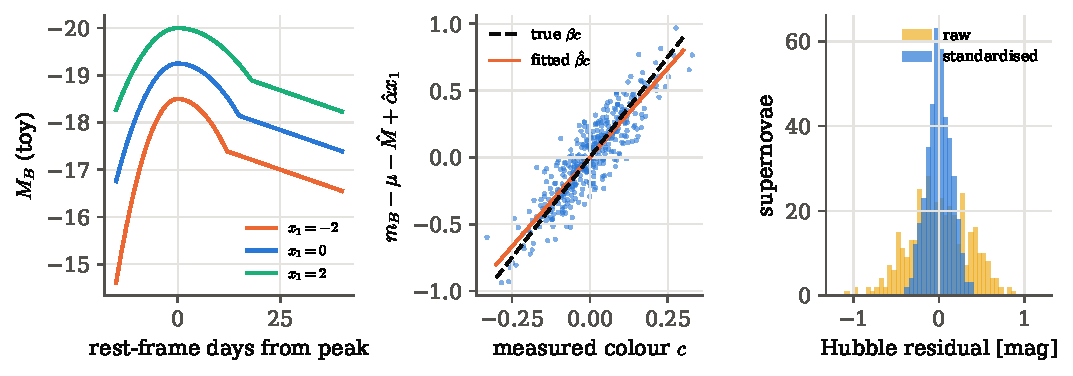
\includegraphics[width=\linewidth]{figures/chT2/sn_standardise.pdf}
\caption{Standardising type~Ia supernovae. Left: toy light curves; the broad one ($x_1=2$) is brighter, the narrow one fainter (the trend is exaggerated for visibility). Middle: after the stretch correction, the residual magnitude grows linearly with the measured colour; the fitted slope (orange) is shallower than the true one (dashed) because the colours are noisy. Right: Hubble residuals before (yellow) and after (blue) the correction.}
\label{T2b:fig:sn-standardise}
\end{figure}

\paragraph{Where the statistics comes back in.} The datum is the model's prediction plus one realisation of the noise, $\mu_{\rm obs}=\mu(z;\params)+\Delta\mu$ with $\Delta\mu\sim\Normal(0,\sigma^2)$. For a trial $\params$ the likelihood asks how plausible the particular noise realisation is that would turn that model's prediction into the magnitudes actually observed; a $\params$ that needs a large, improbable $\Delta\mu$ in every supernova is disfavoured. The residual $\Delta\mu$ is Gaussian in magnitudes, so the likelihood of \cref{ch:03} with the Hubble law, and the $H_0$ estimator built there, apply directly. Fitting $\alpha$, $\beta$, $M$ and the cosmology together is a linear-in-nuisance problem, solved by the least squares of \cref{ch:03} or marginalised in \cref{ch:05}. Correlated systematics (a calibration offset shared by all supernovae from one telescope) enter as a full covariance matrix $\Cmat$, whose use in the likelihood and in the Fisher matrix is the subject of \cref{ch:10}. The hierarchical treatment of latent colours is sampled with the MCMC of \cref{ch:09}.
\section{The distance ladder: why \texorpdfstring{$H_0$}{H0} needs an anchor}
\label{T2b:sec:ladder}

The supernovae of \cref{T2b:sec:snia} are excellent at \emph{relative} distances: this one is $1.8$ times farther than that one. They say nothing, on their own, about how far away either of them is in megaparsecs. The worked problem of \cref{ch:03} found the same thing in the language of likelihoods. In the Hubble law with supernova magnitudes, the absolute magnitude $M$ and $5\log_{10}H_0$ enter only in the combination $M-5\log_{10}H_0$, so the Fisher matrix of the two is singular. Brighter candles in a faster-expanding universe look exactly like fainter candles in a slower one. To measure $H_0$ someone has to tell us $M$, and the only way to do that is to find supernovae in galaxies whose distances are known by other means. Those distances in turn need calibrating, and the chain ends only at geometry. This chain is the \newterm{distance ladder}.

\emph{Where we have met $H_0$ before.} In \cref{3b:sec:hubble} we fitted mock surveys of $100$ supernovae made with $H_0=70$ and an absolute magnitude $M=-19.25$ that we simply declared known, and the maximum-likelihood estimator, the weighted mean of $5\log_{10}H_0$, found $H_0$ to about $0.5$\,km/s/Mpc. \Cref{3b:sec:hubble-degeneracy} then freed $M$, saw the Fisher matrix of $(M,5\log_{10}H_0)$ turn singular, and closed the gap by handing the fit one more number, $M_{\rm cal}\pm0.03$\,mag, from ``the calibrators''; the calibration error then dominated, and the scatter of $\hat H_0$ grew to $1.1$\,km/s/Mpc. Here the parameter, the magnitude likelihood and the degeneracy are the same, and so is the estimator, now written as generalised least squares. What changes is where $M$ comes from: instead of arriving as one number with an assumed error, it is produced by fitting the rungs below, so its error is assembled from parallaxes, Cepheids and calibrator supernovae, and we can ask which rung pays for most of it. The data are still mock, made with $H_0=\TwlHtrue$ to sit near the published value, which is met in \cref{T2b:sec:tension}. The two error bars come out almost equal, $1.1$\,km/s/Mpc in both, because the ladder below delivers $M$ to $0.03$\,mag, the precision the worked problem assumed.

\paragraph{The question.} Which measurements make up the ladder, what does each one measure and with what noise, and how do the errors of the rungs combine into the error on $H_0$?

\subsection{The rungs}

\emph{Rung 1, geometry.} The \newterm{parallax} $p$ of a star is the half-angle through which it appears to move as the Earth goes round the Sun. Its distance is $d=1\,\mathrm{AU}/\tan p$, that is $d=1\,\mathrm{pc}\times(1''/p)$ for small angles \cite[Sec.~8]{Hogg1999}. The Gaia satellite measures parallaxes to some $20\,\mu$as, so a Cepheid at $2$\,kpc ($p=0.5$\,mas) has its distance to $4\%$. Two other geometric anchors reach farther: detached eclipsing binaries in the Large Magellanic Cloud (the stars' sizes from the eclipse timing, their angular sizes from their surface brightness) and the water masers orbiting the black hole in NGC\,4258 (a Keplerian disc whose velocity and proper motion give its physical and angular size). Both give distances to about $1$--$1.5\%$ \cite{Riess2022SH0ES}.

\emph{Rung 2, a stellar standard candle.} \newterm{Cepheids} are pulsating giant stars whose brightness varies with periods of days to months. Brighter Cepheids pulsate more slowly. The \newterm{Leavitt law} \unpack{the period--luminosity relation of Cepheids, a straight line in $\log P$} says
\begin{equation}
  m_{W}=\mu+M_W+b_W\,(\log_{10}P-1),
  \label{T2b:eq:leavitt}
\end{equation}
where $m_W$ is a reddening-free combination of magnitudes in two bands (a ``Wesenheit'' magnitude), $M_W$ the absolute magnitude of a $10$-day Cepheid, and $b_W\approx-3.3$ the slope. The scatter about the line is about $0.25$\,mag per star, but a galaxy contains dozens of Cepheids, so its distance modulus $\mu$ is found to a few hundredths of a magnitude. The alternative second rung is the \newterm{tip of the red giant branch} (TRGB): the brightest red giants are those about to ignite helium in their cores, and the ignition happens at a fixed core mass, so the tip of the giant branch is a standard candle with $M_I\approx-4.05$. Both second rungs are reviewed in \cite[Sec.~IV.A]{Abdalla2022}.

\emph{Rung 3, supernovae in calibrator galaxies.} A few dozen galaxies within $\sim40$\,Mpc have both Cepheids (or a measured TRGB) and a well-observed type~Ia supernova. In each of them the Cepheids give $\mu$, and the supernova gives $m_B$, so $M_B=m_B-\mu$. SH0ES uses $42$ supernovae in $37$ such hosts \cite{Riess2022SH0ES}.

\emph{Rung 4, the Hubble flow.} Supernovae at $0.023<z<0.15$ are far enough that peculiar velocities matter little (\eqref{T2b:eq:mu-pec}) and near enough that the distance depends on the cosmology only through the deceleration parameter $q_0$ \unpack{$q_0=-\ddot aa/\dot a^2$ today, about $-0.55$ in $\Lambda$CDM}. What fixes that dependence? Expand the comoving distance $D_C=c\int_0^z\dd z'/H(z')$ to second order with $H(z)\approx H_0[1+(1+q_0)z]$, and use $D_L=(1+z)D_C$ for a flat universe \cite[eqs.~(15), (21)]{Hogg1999}:
\begin{align}
  D_L
  &\eqby{1}(1+z)\,\frac{c}{H_0}\int_0^z\big[1-(1+q_0)z'\big]\,\dd z'\nonumber\\
  &\eqby{2}(1+z)\,\frac{c}{H_0}\Big[z-\frac{1+q_0}{2}z^2\Big]
  \eqby{3}\frac{cz}{H_0}\Big[1+\frac{1-q_0}{2}z\Big]+O(z^3).
  \label{T2b:eq:dl-q0}
\end{align}
\begin{explain}
  \item How fast does $H$ change with redshift? Both $H$ and $z$ change with time, so divide their rates of change. The definition of $q$ gives $\dot H=\ddot a/a-\dot a^2/a^2=-H^2(1+q)$, and $1+z=1/a$ gives $\dot z=-\dot a/a^2=-(1+z)H$. Then
        \[
          \frac{\dd H}{\dd z}=\frac{\dot H}{\dot z}=\frac{-H^2(1+q)}{-(1+z)H}=\frac{H(1+q)}{1+z}
          \;\xrightarrow{\;z=0\;}\;(1+q_0)H_0 ,
        \]
        so to first order $H(z)\approx H_0[1+(1+q_0)z]$, and $1/(1+\epsilon)\approx1-\epsilon$ gives $1/H(z)\approx H_0^{-1}[1-(1+q_0)z]$.
  \item Integrate term by term.
  \item Multiply out: $(1+z)\big(z-\tfrac{1+q_0}{2}z^2\big)=z+z^2-\tfrac{1+q_0}{2}z^2+O(z^3)$.
\end{explain}
What does a Hubble-flow supernova then tell us? Its apparent magnitude is its absolute magnitude plus its distance modulus \eqref{T2b:eq:mu}, and \eqref{T2b:eq:dl-q0} gives the distance. The logarithm of a product is a sum of logarithms, which splits the known part from the unknown one:
\begin{align}
  m_{B,i}
  &\eqby{1}M_B+5\log_{10}\frac{D_L(z_i)}{\mathrm{Mpc}}+25\nonumber\\
  &\eqby{2}M_B+5\log_{10}\Big\{cz_i\Big[1+\frac{1-q_0}{2}z_i\Big]\Big\}+25-5\log_{10}H_0
  \eqby{3}M_B+x_i-a ,
  \label{T2b:eq:mb-hf}
\end{align}
with $x_i\equiv5\log_{10}\{cz_i[1+\frac12(1-q_0)z_i]\}+25$ and $a\equiv5\log_{10}H_0$ ($c$ in km/s and $H_0$ in km/s/Mpc, so that $D_L$ is in Mpc).
\begin{explain}
  \item $m=M+\mu$, with $\mu$ from \eqref{T2b:eq:mu}.
  \item Substitute \eqref{T2b:eq:dl-q0} and use $\log(XY/H_0)=\log X+\log Y-\log H_0$.
  \item Name the pieces: $x_i$ is computed from the measured redshift alone (with $q_0$ from the cosmology, a small correction at these redshifts); $a$ is the one unknown that carries $H_0$.
\end{explain}
Here the degeneracy of \cref{ch:03} is visible: only $M_B-a$ appears.

\begin{figure}[htbp]
\centering
\begin{tikzpicture}[scale=0.82,transform shape,
  rung/.style={draw=accent,rounded corners=2pt,fill=ideabg,align=center,font=\small,
               minimum width=3.3cm,minimum height=1.05cm,inner sep=2pt},
  par/.style={font=\small,text=fibreorange},
  arr/.style={->,thick,accent}]
  \node[rung] (r1) at (0,0) {anchors: parallax,\\ masers, eclipsing binaries\\ \textcolor{fibreorange}{fix $\mu_{\rm anc}$}};
  \node[rung] (r2) at (3.9,1.5) {Cepheids / TRGB\\ in the anchors\\ \textcolor{fibreorange}{fix $M_W,\,b_W$}};
  \node[rung] (r3) at (7.8,3.0) {Cepheids + SN Ia\\ in calibrator hosts\\ \textcolor{fibreorange}{fix $M_B$}};
  \node[rung] (r4) at (11.7,4.5) {SN Ia in the\\ Hubble flow\\ \textcolor{fibreorange}{fix $5\log_{10}H_0$}};
  \draw[arr] (r1.east) -- (r2.south);
  \draw[arr] (r2.east) -- (r3.south);
  \draw[arr] (r3.east) -- (r4.south);
  \draw[faint,->] (-1.6,-1.2) -- (13.4,-1.2) node[right,font=\footnotesize,text=softgray] {distance};
  \foreach \x/\t in {0/{$\lesssim 8$\,kpc, 50\,kpc, 7.6\,Mpc},7.8/{$\lesssim40$\,Mpc},11.7/{$100$--$600$\,Mpc}}
    \node[font=\footnotesize,text=softgray] at (\x,-1.5) {\t};
\end{tikzpicture}
\caption{The distance ladder. Each rung measures distances to the objects of the next, and each pair of neighbouring rungs shares a parameter (orange): the anchor distances calibrate the Cepheid law, the Cepheids give the distances of the calibrator hosts and hence the supernova absolute magnitude $M_B$, and $M_B$ turns Hubble-flow magnitudes into $H_0$. The grey scale gives the typical distances of each rung.}
\label{T2b:fig:ladder}
\end{figure}

\subsection{One linear model for the whole ladder}

Each measurement on every rung is a sum of unknowns plus noise. A geometric measurement says $\hat\mu_{\rm anc}=\mu_{\rm anc}+\text{noise}$. A Cepheid says \eqref{T2b:eq:leavitt}. A calibrator supernova says $m_B=\mu_{\rm cal}+M_B+\text{noise}$, and a Hubble-flow supernova says $m_B-x=M_B-a+\text{noise}$ by \eqref{T2b:eq:mb-hf}. None of them multiplies two unknowns together, so the whole ladder is one linear model.

\emph{The smallest ladder first.} Take two anchors, one calibrator host and one Hubble-flow supernova, with one Cepheid in each galaxy, and treat the Cepheid slope $b_W$ as known, so that the term $b_W(\log_{10}P-1)$ can be moved to the data side. The unknowns are the two anchor moduli, the calibrator modulus, the two absolute magnitudes and $a$, collected as $\params=(\mu_1,\mu_2,\mu_{\rm cal},M_W,M_B,a)$. Write each measurement as one row: its coefficients on the unknowns go into a row of the matrix $A$, and the measured number into $\bm y$,
\[
  \underbrace{\begin{pmatrix}
    \hat\mu_1\\ \hat\mu_2\\ m_{W,1}-b_W(\log_{10}P_1-1)\\ m_{W,2}-b_W(\log_{10}P_2-1)\\ m_{W,\rm cal}-b_W(\log_{10}P_{\rm cal}-1)\\ m_{B,\rm cal}\\ m_{B,\rm HF}-x
  \end{pmatrix}}_{\bm y}
  =
  \underbrace{\begin{pmatrix}
    1&0&0&0&0&0\\
    0&1&0&0&0&0\\
    1&0&0&1&0&0\\
    0&1&0&1&0&0\\
    0&0&1&1&0&0\\
    0&0&1&0&1&0\\
    0&0&0&0&1&-1
  \end{pmatrix}}_{A}
  \begin{pmatrix}\mu_1\\ \mu_2\\ \mu_{\rm cal}\\ M_W\\ M_B\\ a\end{pmatrix}
  +\bm n .
\]
Read down a column to see how the rungs are tied. The column of $M_W$ has a $1$ in every Cepheid row, in the anchors and in the calibrator alike, so the anchors' geometry reaches the calibrator through it. The column of $M_B$ has a $1$ in both supernova rows, so the calibrator passes its information to the Hubble flow. The column of $\mu_{\rm cal}$ joins the calibrator's Cepheid to its supernova. Only the last row involves $a$.

The real ladder is this pattern repeated: $N_{\rm anc}$ anchors and $N_{\rm cal}$ calibrator hosts, each with its own modulus column, dozens to hundreds of Cepheid rows per galaxy, one supernova row per calibrator, a row for each Hubble-flow supernova, and a seventh kind of column for $b_W$, whose entry in a Cepheid row is that star's $\log_{10}P-1$. Stack all of them as $\bm y=A\params+\bm n$ with noise covariance $\Cmat$. The generalised least-squares solution of \cref{ch:03} is
\begin{equation}
  \hat\params=(A\T\Cmat^{-1}A)^{-1}A\T\Cmat^{-1}\bm y,\qquad
  \Cov(\hat\params)=(A\T\Cmat^{-1}A)^{-1}=\Fish^{-1},
  \label{T2b:eq:gls}
\end{equation}
and the matrix $A\T\Cmat^{-1}A$ is exactly the Fisher matrix $\Fish$ of this linear Gaussian model (\cref{ch:10}). The ladder is ``one big fit'': the information flows up the rungs through the shared parameters, and so do the errors.

\paragraph{How the errors add up.} It helps to see the answer rung by rung before letting the matrix do it. The ingredients, one at a time: there are $N_{\rm anc}$ anchors, each with a geometric error $\sigma_{\rm geo}$ (in magnitudes of distance modulus) and $n_A$ Cepheids; there are $N_{\rm cal}$ calibrator hosts, each with $n_C$ Cepheids and one supernova; a single Cepheid scatters about the Leavitt law by $\sigma_{\rm ceph}$, a single calibrator supernova by $\sigma_{\rm SN}$; and there are $N_{\rm HF}$ Hubble-flow supernovae, each of scatter $\sigma_{\rm HF}$. Take the Cepheid slope $b_W$ as known (it is fixed by thousands of Cepheids, so its error is small) and follow the estimate up the ladder, one rung at a time.

\emph{One anchor.} Average its $n_A$ Cepheids, after removing the known slope term, and subtract the geometric modulus. By \eqref{T2b:eq:leavitt} what is left is $M_W$:
\[
  \hat M_W^{(j)}=\overline{\big[m_W-b_W(\log_{10}P-1)\big]}_{\,j}-\hat\mu_{{\rm anc},j},
  \qquad
  \Var\hat M_W^{(j)}=\frac{\sigma_{\rm ceph}^2}{n_A}+\sigma_{\rm geo}^2 ,
\]
because the mean of $n_A$ independent Cepheids has variance $\sigma_{\rm ceph}^2/n_A$, and the geometric error is independent of the Cepheids. \emph{Then all anchors.} The $N_{\rm anc}$ anchors are independent of one another, so their average $\hat M_W$ has $1/N_{\rm anc}$ of this variance. That is line 1 of \eqref{T2b:eq:ladder-budget} below.

\emph{One calibrator.} Its Cepheids give its modulus as $\hat\mu_{{\rm cal},i}=\overline{[m_W-b_W(\log_{10}P-1)]}_{\,i}-\hat M_W$, and its supernova then gives
\[
  \hat M_B^{(i)}=m_{B,i}-\hat\mu_{{\rm cal},i}
  =\underbrace{m_{B,i}-\overline{\big[m_W-b_W(\log_{10}P-1)\big]}_{\,i}}_{\text{private to host }i}
  \;+\;\underbrace{\hat M_W}_{\text{common to all hosts}} .
\]
The private part has variance $\sigma_{\rm SN}^2+\sigma_{\rm ceph}^2/n_C$ and is independent from host to host. The common part is the \emph{same} number in every host: if $\hat M_W$ came out $0.02$\,mag too bright, every calibrator inherits the same $0.02$\,mag. \emph{Average the $N_{\rm cal}$ hosts.} The private errors average down, to $1/N_{\rm cal}$ of their variance. The common error does not: the average of $N_{\rm cal}$ copies of the same offset is that offset. So
\[
  \Var\hat M_B=\Var\Big(\overline{\text{private}}\Big)+\Var(\hat M_W)
  =\frac{1}{N_{\rm cal}}\Big(\sigma_{\rm SN}^2+\frac{\sigma_{\rm ceph}^2}{n_C}\Big)+\Var(\hat M_W),
\]
the two parts adding because the hosts' own errors are independent of the anchors'. That is line 2.

\emph{The Hubble flow, the same way.} By \eqref{T2b:eq:mb-hf} each Hubble-flow supernova gives $\hat a^{(k)}=\hat M_B-(m_{B,k}-x_k)$. The term in brackets is private, with variance $\sigma_{\rm HF}^2$; $\hat M_B$ is common to all of them. Averaging $N_{\rm HF}$ supernovae shrinks only the private part. Collecting the three rungs,
\begin{align}
  \Var(\hat M_W)&\eqby{1}\frac{1}{N_{\rm anc}}\Big(\sigma_{\rm geo}^2+\frac{\sigma_{\rm ceph}^2}{n_A}\Big),\nonumber\\
  \Var(\hat M_B)&\eqby{2}\Var(\hat M_W)+\frac{1}{N_{\rm cal}}\Big(\sigma_{\rm SN}^2+\frac{\sigma_{\rm ceph}^2}{n_C}\Big),\nonumber\\
  \Var(\hat a)&\eqby{3}\Var(\hat M_B)+\frac{\sigma_{\rm HF}^2}{N_{\rm HF}},\qquad
  \frac{\sigma_{H_0}}{H_0}\eqby{4}\frac{\ln10}{5}\,\sqrt{\Var(\hat a)} .
  \label{T2b:eq:ladder-budget}
\end{align}
\begin{explain}
  \item One anchor gives $\sigma_{\rm geo}^2+\sigma_{\rm ceph}^2/n_A$; $N_{\rm anc}$ independent anchors divide it by $N_{\rm anc}$.
  \item The calibrators' private errors average down; the error of $\hat M_W$ is common to all of them and passes through whole.
  \item The same split one rung higher: the error of $\hat M_B$ is common to all Hubble-flow supernovae.
  \item $H_0=10^{a/5}=e^{(\ln10/5)a}$, so $\delta H_0/H_0=\delta\ln H_0=(\ln10/5)\,\delta a$.
\end{explain}
Every rung adds its own variance, and the variance of a lower rung is never diluted by more objects on a higher one. A million Hubble-flow supernovae cannot fix a bad anchor.

\paragraph{Example: the error budget of a SH0ES-sized ladder.}
Take $N_{\rm anc}=\TwlNanc$ anchors with $\sigma_{\rm geo}=\TwlSigGeo$\,mag and $n_A=\TwlNcephAnc$ Cepheids each, $N_{\rm cal}=\TwlNcal$ calibrators with $n_C=\TwlNcephCal$ Cepheids each, $\sigma_{\rm ceph}=\TwlSigCeph$, $\sigma_{\rm SN}=\TwlSigSn$, and $N_{\rm HF}=\TwlNhf$ Hubble-flow supernovae with $\sigma_{\rm HF}=\TwlSigHf$. Substituting line 1 into line 2 and line 2 into line 3 of \eqref{T2b:eq:ladder-budget} writes $\Var(\hat a)$ as five separate terms, one per source of noise:
\begin{align*}
  \Var(\hat a)&=\underbrace{\frac{\sigma_{\rm geo}^2}{N_{\rm anc}}}_{\text{anchor geometry}}
  +\underbrace{\frac{\sigma_{\rm ceph}^2}{N_{\rm anc}n_A}}_{\text{anchor Cepheids}}
  +\underbrace{\frac{\sigma_{\rm SN}^2}{N_{\rm cal}}}_{\text{calibrator SNe}}
  +\underbrace{\frac{\sigma_{\rm ceph}^2}{N_{\rm cal}n_C}}_{\text{calibrator Cepheids}}
  +\underbrace{\frac{\sigma_{\rm HF}^2}{N_{\rm HF}}}_{\text{Hubble flow}}\\
  &=\underbrace{\frac{0.03^2}{3}}_{3.0\times10^{-4}}+\underbrace{\frac{0.25^2}{300}}_{2.1\times10^{-4}}
  +\underbrace{\frac{0.13^2}{40}}_{4.2\times10^{-4}}+\underbrace{\frac{0.25^2}{1200}}_{0.5\times10^{-4}}
  +\underbrace{\frac{0.14^2}{280}}_{0.7\times10^{-4}}=1.05\times10^{-3},
\end{align*}
where $300=N_{\rm anc}n_A=3\times100$ and $1200=N_{\rm cal}n_C=40\times30$. So $\sigma_a=0.032$\,mag and $\sigma_{H_0}/H_0=0.4605\times0.032=\TwlFracApprox\%$. The calibrator supernovae and the anchors dominate; the Hubble flow, with its $280$ supernovae, contributes least. Doubling the number of calibrators is worth far more than doubling the Hubble-flow sample.

\paragraph{The experiment.} \pyname{07_distance_ladder.py} builds the full matrix $A$ for this ladder ($\TwlNpar$ parameters, one row per measurement) and solves \eqref{T2b:eq:gls}:

\pyfile[firstline=44,lastline=72,firstnumber=44]{code/chT2/07_distance_ladder.py}{The ladder as one linear model, solved by generalised least squares}

\noindent Each call to \pyname{add} writes one row of $A$: its nonzero entries say which parameters that measurement involves. Lines 53, 56 and 63 are the three kinds of shared-parameter rows that tie the rungs together. One mock ladder gives $H_0=\TwlHhat\pm\TwlHerr$ (true value $\TwlHtrue$), a $\TwlFrac\%$ measurement, the same as the rung-by-rung estimate. Over $\TwlNmc$ independent mock ladders the estimates average $\TwlMcMean$ with standard deviation $\TwlMcSd$, while the quoted errors average $\TwlMcErr$, and the $1\sigma$ interval covers the truth in $\TwlCover$ of them: the inverse Fisher matrix is the true covariance here, as it must be for a linear Gaussian model. \Cref{T2b:fig:ladder-mc} shows the budget as the number of calibrators grows: the error falls from $\TwlFracFive\%$ with $5$ calibrators to $\TwlFracOneSixty\%$ with $160$, and then flattens on the anchor floor of $\TwlCanc\%$.

\begin{figure}[htbp]
\centering
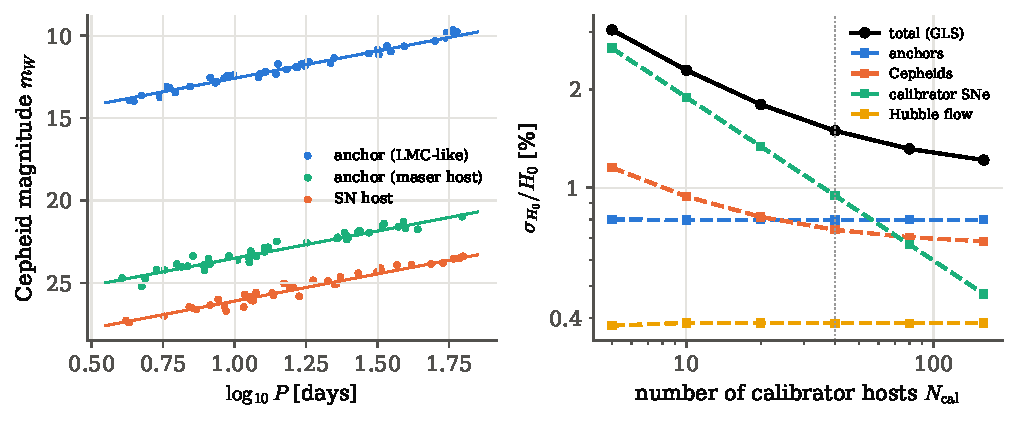
\includegraphics[width=0.95\linewidth]{figures/chT2/distance_ladder.pdf}
\caption{Left: mock Cepheids in two anchors and one supernova host follow parallel Leavitt laws; their vertical offsets are the differences of distance modulus. Right: the fractional error on $H_0$ from the full fit (black) and the contribution of each rung (computed by making that rung noiseless and subtracting in quadrature), against the number of calibrator hosts. The dotted line marks the default ladder.}
\label{T2b:fig:ladder-mc}
\end{figure}

\subsection{The real ladder and the Hubble tension}
\label{T2b:sec:tension}

\emph{Where we have met $H_0$ before.} Every $H_0$ so far was made up by us: the $70$ of the mock supernovae of \cref{3b:sec:hubble}, where $M$ was known, and the $\TwlHtrue$ of the mock ladder just built, recovered as $\TwlHhat\pm\TwlHerr$. In both the truth was known, and the only question was whether the estimator found it and whether its error bar covered it. Here the numbers are published measurements, the truth is not known, and the question becomes whether two of them can be measurements of the same constant. The ladder side is the same construction as above, the Hubble-flow fit of \cref{3b:sec:hubble-degeneracy} with $M$ supplied by the rungs, and its published error, $1.04$, is close to our mock $\TwlHerr$ because the mock was built to be SH0ES-sized. The other side is calibrated by something else entirely: no candle, but the sound horizon at recombination, whose angle on the sky fixes $H_0$ as a parameter derived from the CMB fit (\cref{10a:sec:cmb-planck}). The degeneracy of \cref{3b:sec:hubble-degeneracy} reappears as the way to read the disagreement: since supernovae fix only $M-5\log_{10}H_0$, a gap in $H_0$ is a gap in the luminosity of the candle. \Cref{9c:sec:importance} later adds the ladder value to a CMB chain by reweighting, and \cref{11c:sec:h0-routes} sets all the routes side by side.

Two kinds of measurement give $H_0$, and they answer different questions. The SH0ES team asks: \emph{how fast are galaxies around us receding now, per megaparsec of distance, with distances from geometry alone?} Their ladder is the one built above, and the only physics it assumes is in the rungs themselves (parallax, the Leavitt law, standardised supernovae); no cosmological model enters except the small $q_0$ term of \eqref{T2b:eq:dl-q0}. The Planck team asks a different question: \emph{which $\Lambda$CDM universe produces the pattern of hot and cold spots we see in the CMB, emitted at $z\approx1100$?} $H_0$ is one of the outputs of that fit. It is not measured locally but predicted forward, by running the fitted model from $z\approx1100$ to today. So the two numbers are not two measurements of the same quantity by two instruments; one is a local measurement, the other a prediction of $\Lambda$CDM. If they disagree, either a rung of the ladder is wrong or the model that carries the CMB to today is.

\begin{center}
\small
\begin{tabular}{@{}lll@{}}
\toprule
method & $H_0$ [km/s/Mpc] & what it assumes\\
\midrule
SH0ES, Cepheid ladder & $73.04\pm1.04$ & local geometry and the physics of each rung\\
Planck, CMB & $67.36\pm0.54$ & flat $\Lambda$CDM from $z\approx1100$ to today\\
CCHP TRGB ladder & $69.8\pm1.7$ & local geometry, red giants in place of Cepheids\\
\bottomrule
\end{tabular}
\end{center}

\noindent The values are from \cite{Riess2022SH0ES}, \cite[Table~2]{Planck2018VI} (TT,TE,EE+lowE+lensing) and \cite[Sec.~IV.A]{Abdalla2022}, which quotes the TRGB value of the Carnegie--Chicago Hubble Program (CCHP) of Freedman et al. The TRGB ladder lands between the other two.

\emph{How many standard deviations apart?} The two measurements are independent, so the variance of their difference is the sum of their variances (\cref{ch:04}), and
\[
  \frac{73.04-67.36}{\sqrt{1.04^2+0.54^2}}=\frac{5.68}{1.17}=4.8 ,
\]
the ``about $5\sigma$'' of \cite[Sec.~IV.A]{Abdalla2022}.

\emph{The same gap in magnitudes.} By \eqref{T2b:eq:mb-hf} the Hubble-flow supernovae fix only $M_B-a=M_B-5\log_{10}H_0$. Hold that combination fixed and raise $H_0$ by a factor $r$: $a$ grows by $5\log_{10}r$, so $M_B$ must grow by the same amount. A larger $M_B$ means intrinsically fainter supernovae, which for the same apparent magnitude must be nearer, and nearer galaxies with the same redshifts mean a faster expansion. For the two values,
\[
  \Delta M_B=5\log_{10}\frac{73.04}{67.36}=5\times0.035=0.18\ \text{mag}:
\]
the whole tension is equivalent to a disagreement of $0.18$\,mag about how bright type~Ia supernovae are, with the ladder's supernovae the fainter ones. That is why it is cleanest to carry the ladder into a cosmological fit not as a value of $H_0$ but as a Gaussian prior on $M_B$ \cite[Sec.~IV.E, eq.~(1)]{Abdalla2022}: the ladder calibrates $M_B$, and $H_0$ then follows from the supernovae together with whatever cosmological model is being tested.

\paragraph{Example: can a local void explain it?} Suppose we live inside a sphere whose mean density is below the cosmic mean, with $\delta$ the mean density contrast inside the sphere ($\delta<0$ for a void). Why would the local expansion be faster? The denser surroundings pull the matter at the edge of the sphere outwards, and the sphere has less mass inside to hold it back, so matter streams out of the void. On top of the Hubble flow there is an outflow, and someone inside who measures recession velocities sees them grow faster with distance than the global $H_0$: the local rate is $H_0+\delta H$ with $\delta H>0$. How much faster? Linear continuity, $\dot\delta=-\nabla\cdot\bm v$ for the peculiar velocity $\bm v$ (derived in \cref{T2b:sec:tracers}, \eqref{T2b:eq:continuity}), and the growth rate $\dot\delta=fH\delta$ with $f\approx\Omega_m^{0.55}\approx0.53$ give
\begin{align}
  \frac{\delta H_0}{H_0}
  &\eqby{1}\frac{\nabla\cdot\bm v}{3H_0}
  \eqby{2}-\frac{\dot\delta}{3H_0}
  \eqby{3}-\frac{f}{3}\,\delta ,
  \label{T2b:eq:void}
\end{align}
\begin{explain}
  \item The extra outflow grows in proportion to distance, $\bm v=\delta H\,\bm r$, which is what a change $\delta H$ of the local Hubble rate means. Its divergence is $\nabla\cdot\bm v=\partial_xv_x+\partial_yv_y+\partial_zv_z=3\,\delta H$.
  \item Continuity: matter flowing out of the sphere lowers its density, $\dot\delta=-\nabla\cdot\bm v$.
  \item Linear growth, $\delta\propto D(t)$, so $\dot\delta=(\dd\ln D/\dd\ln a)(\dot a/a)\,\delta=fH\delta$, with $H=H_0$ today.
\end{explain}
which is Abdalla et al.'s eq.~(2) \cite[Sec.~IV.F]{Abdalla2022}. The sign is as expected: $\delta<0$ gives $\delta H_0>0$. How empty would the void have to be? The gap between the ladder and the CMB is $(73.04-67.36)/67.36=8.4\%$, about $8\%$, so
\[
  0.08=\frac{0.53}{3}\,|\delta|\quad\Longrightarrow\quad|\delta|=\frac{3\times0.08}{0.53}=0.45 ,
\]
a region almost half empty, over the whole volume probed by the Hubble-flow supernovae, out to $z=0.15$ or some $600$\,Mpc. Density fluctuations on such scales are at the percent level, and theory and simulations put the expected scatter of the local $H_0$ at $0.5$--$1\%$ \cite[Sec.~IV.F]{Abdalla2022}, an order of magnitude too small.

\paragraph{Where the statistics comes back in.} The ladder is generalised least squares (\cref{ch:03}), and its covariance is the inverse Fisher matrix (\cref{ch:10}). Testing whether two measurements of $H_0$ agree is a hypothesis test on their difference (\cref{ch:04}). Using the ladder as a prior on $M_B$ is Bayesian combination of independent data (\cref{ch:05}). Peculiar velocities and the local Hubble flow are taken up again as data in their own right in \cref{11c:sec:virgo}, and the local cosmic variance of $H_0$, the careful version of the void estimate above, in \cref{11c:sec:cosmicvar}.
\section{Selection effects: what a flux limit does to a sample}
\label{T2b:sec:malmquist}

Every survey has a faintest object it can detect. Close to that limit the survey does not see a fair sample of what is there: it sees the objects that happened to be brighter than average, because their fainter siblings at the same distance were lost. Treat the survivors as typical, and their distances come out too small. At high redshift, where most of the cosmological information sits, the supernovae look brighter than the model predicts, and the fit moves the cosmological parameters to make them so.

The plain claim is that ``the mean absolute magnitude of type~Ia supernovae is $M_0$''. The everyday question is: \emph{if I average the absolute magnitudes of the supernovae in my catalogue, do I get $M_0$?} The question hides a sampling rule. ``The mean'' of the luminosity function is an average over supernovae drawn uniformly \emph{per unit volume}. A catalogue is drawn by a different rule: a supernova enters it if its apparent magnitude is below the limit. Change the sampling rule and the distribution changes, exactly as the distribution of an oscillator's position changes when we sample it uniformly in position rather than in time. The physics of the explosions is the same in both cases; what differs is how the objects were selected.

Selection is conditioning, and conditioning has a picture (\cref{1a:fig:shrink}, \cref{5a:sec:shrink}). Draw every supernova that went off in the survey volume as a point in a rectangle: that rectangle is the full sample space, and the luminosity function describes how the points are spread over it. Detection draws a line through the rectangle: on one side are the supernovae brighter than the limit, $m<m_{\rm lim}$, on the other the ones we never see. Once we know a supernova is in the catalogue, everything on the far side of the line is discarded. The surviving region becomes the new sample space, and every probability is measured again as a fraction of its area. If the survivors are a fraction $P(\text{detected})$ of the whole, every probability of the full population is divided by that fraction. The mean of the survivors, and the likelihood of what they show us, are both computed in the shrunken space. Nothing about an individual explosion has changed; only the region against which it is measured has.

\paragraph{The question.} For candles with a Gaussian spread of absolute magnitudes, (1) what is the mean absolute magnitude of the ones a flux-limited survey detects, (2) how biased are the Hubble residuals near the limit, and (3) what likelihood removes the bias?

\subsection{The classical Malmquist bias}

The inputs are three.
\begin{enumerate}[itemsep=1pt]
  \item \emph{Physical:} the candles are spread uniformly through a static Euclidean space, with number density $n$.
  \item \emph{Physical:} their absolute magnitudes follow a Gaussian \newterm{luminosity function} \unpack{the distribution of absolute magnitudes among the candles} $\varphi(M)=\Normal(M_0,\sigma^2)$, the same everywhere and independent of position.
  \item \emph{Selection:} we look at the objects whose apparent magnitude lies in a narrow interval $[m,m+\dd m]$.
\end{enumerate}

\emph{What we observed} is an object of apparent magnitude $m$. \emph{What could have produced it?} Any absolute magnitude $M$, placed at the distance modulus $\mu=m-M$ that makes it appear at $m$. \emph{How likely is each candidate?} It is the probability of drawing that $M$ from the luminosity function, times the number of places at that distance where the object could be. The number of objects in a shell of radius $r$ and thickness $\dd r$ is $n\,4\pi r^2\dd r$, and $r$ is tied to $\mu$ by $r=10^{\mu/5+1}$\,pc. So
\begin{align}
  \dd N(M,\mu)
  &\eqby{1}n\,\varphi(M)\,\dd M\;4\pi r^2\,\frac{\dd r}{\dd\mu}\,\dd\mu
  \eqby{2}n\,\varphi(M)\,\dd M\;4\pi\frac{\ln10}{5}\,r^3\,\dd\mu
  \;\propto\;\varphi(M)\,10^{0.6\mu}\,\dd M\,\dd\mu ,\nonumber\\
  p(M\given m)
  &\eqby{3}\frac{\varphi(M)\,10^{0.6(m-M)}}{\int\varphi(M')\,10^{0.6(m-M')}\dd M'}
  \eqby{4}\Normal\big(M_0-0.6\ln10\,\sigma^2,\;\sigma^2\big).
  \label{T2b:eq:malmquist}
\end{align}
\begin{explain}
  \item Independence of luminosity and position (inputs 1 and 2): the joint density is the product. Change variable from $r$ to $\mu$.
  \item $r\propto10^{\mu/5}$, so $\dd r/\dd\mu=(\ln10/5)\,r$, and $r^3\propto10^{3\mu/5}$.
  \item Fix $m$ (input 3): $\mu=m-M$, and $\dd\mu=\dd m$ does not depend on $M$. Normalise over $M$.
  \item $10^{-0.6M}=e^{-0.6\ln10\,M}$. Multiply it into the Gaussian and complete the square: $-\frac{(M-M_0)^2}{2\sigma^2}-kM=-\frac{(M-M_0+k\sigma^2)^2}{2\sigma^2}+\text{const}$ with $k=0.6\ln10$.
\end{explain}

\begin{keyidea}[Malmquist bias]
In a flux-limited sample of candles spread uniformly in Euclidean space, the detected objects are on average brighter than the luminosity function by
\[
  \langle M\rangle_{\rm det}-M_0=-0.6\ln10\;\sigma^2=-1.382\,\sigma^2 ,
\]
at every apparent magnitude. The reason is volume: there is more space at large distances, so an object at a given $m$ is more likely to be a bright one far away than a faint one nearby.
\end{keyidea}

The shift does not depend on $m$ or on where the limit is, so the whole flux-limited sample shares it. The size matters. For raw supernovae, $\sigma=0.4$\,mag, the shift is
\[
  \langle M\rangle_{\rm det}-M_0=-1.382\times0.4^2=-0.22\ \text{mag}.
\]
\emph{Which way does that move a distance?} We infer the distance modulus as $\mu_{\rm inf}=m-M_0$. The detected supernovae really have, on average, $M=M_0-0.22$, so their true modulus is $\mu=m-M_0+0.22$, and the inferred one is too small by $0.22$: a candle that is brighter than we assume looks closer than it is. Since $D_L\propto10^{\mu/5}$ by \eqref{T2b:eq:mu},
\[
  \frac{D_{\rm inf}}{D_{\rm true}}=10^{-0.22/5}=10^{-0.044}=0.90 ,
\]
so distances come out $10\%$ too small. After standardisation, $\sigma=0.12$\,mag, the shift is $1.382\times0.12^2=0.020$\,mag and $10^{-0.020/5}=0.99$, a $1\%$ distance error, which is still as large as the statistical error of a modern survey. The key idea depends on its inputs. In an expanding universe the volume does not grow as $r^3$; if the spread $\sigma$ itself depends on distance, or the luminosity function has a non-Gaussian tail, the number changes. The mechanism, a luminosity function reweighted by the volume where each luminosity can be seen, does not.

\subsection{Near the limit: a truncated Gaussian}

Now the version that matters for a supernova Hubble diagram. At redshift $z$, the model predicts a mean apparent magnitude $\bar m(z;\params)=M_B+\mu(z;\params)$, and the observed magnitudes scatter about it, $m=\bar m+\epsilon$ with $\epsilon\sim\Normal(0,\sigma^2)$. The survey keeps a supernova only if $m<m_{\rm lim}$. \emph{What is the mean residual of the supernovae it keeps?} With $t\equiv(m_{\rm lim}-\bar m)/\sigma$ the distance of the limit from the mean in units of $\sigma$, and $\phi$, $\Phi$ the standard normal density and distribution function,
\begin{align}
  \E[\epsilon\given\epsilon<t\sigma]
  &\eqby{1}\frac{\int_{-\infty}^{t\sigma}\epsilon\,\frac1\sigma\phi(\epsilon/\sigma)\,\dd\epsilon}{\Phi(t)}
  \eqby{2}\frac{-\sigma\big[\phi(\epsilon/\sigma)\big]_{-\infty}^{t\sigma}}{\Phi(t)}
  \eqby{3}-\sigma\,\frac{\phi(t)}{\Phi(t)} .
  \label{T2b:eq:trunc-mean}
\end{align}
\begin{explain}
  \item Conditional expectation: integrate over the kept region and divide by its probability $\Prob(\epsilon<t\sigma)=\Phi(t)$. The division is the renormalisation of the shrunken sample space: the kept region has total probability $\Phi(t)$, and dividing by it makes the probabilities inside it add up to one again.
  \item $\frac{\dd}{\dd\epsilon}\phi(\epsilon/\sigma)=-\frac{\epsilon}{\sigma^2}\phi(\epsilon/\sigma)$, so $\epsilon\,\phi(\epsilon/\sigma)/\sigma$ is $-\sigma$ times the derivative of $\phi(\epsilon/\sigma)$.
  \item $\phi$ vanishes at $-\infty$.
\end{explain}
Two cases give the result a size. Far from the limit ($t\gg1$), $\Phi(t)\to1$ (almost nothing is cut) and $\phi(t)\to0$ (the Gaussian has no weight there), so the bias vanishes. Where half the supernovae are lost ($t=0$), $\phi(0)=1/\sqrt{2\pi}$ and $\Phi(0)=1/2$, so the bias is $-\sigma\cdot2/\sqrt{2\pi}=-\sigma\sqrt{2/\pi}=-0.80\,\sigma$. Beyond that ($t<0$) it grows without bound. \Cref{T2b:fig:malmquist-cartoon} shows the mechanism at three distances.

\begin{figure}[htbp]
\centering
\begin{tikzpicture}[x=1cm,y=1cm]
  \draw[->,faint] (0,-2.2) -- (9.6,-2.2) node[right,font=\small,text=black] {distance $\mu$};
  \draw[->,faint] (0,-2.2) -- (0,2.4) node[above,font=\small,text=black] {brighter};
  \draw[faint,dashed] (0,0) -- (9.4,0) node[right,font=\footnotesize,text=softgray] {$M_0$};
  \draw[bdry] (5.6,-2.03) -- (9.0,2.5) node[above,font=\footnotesize,text=bdryred] {$m=m_{\rm lim}$};
  \foreach \X/\Yl/\Ym in {3.0/-5.5/0.0, 7.125/0.0/0.479, 8.2/1.433/1.63}{
    \begin{scope}
      \clip (\X,\Yl) rectangle (\X+1.2,2.3);
      \fill[formblue!35] (\X,-2.0) -- plot[domain=-2.0:2.0,samples=60,smooth] ({\X+0.75*exp(-(\x)^2/0.72)},\x) -- (\X,2.0) -- cycle;
    \end{scope}
    \draw[formblue,thick] plot[domain=-2.0:2.0,samples=60,smooth] ({\X+0.75*exp(-(\x)^2/0.72)},\x);
    \draw[faint] (\X,-2.0) -- (\X,2.0);
    \draw[fibreorange,very thick] (\X-0.15,\Ym) -- (\X+0.3,\Ym);
  }
  \node[font=\footnotesize,align=center] at (3.5,-2.6) {all detected};
  \node[font=\footnotesize,align=center] at (7.1,-2.6) {half detected};
  \node[font=\footnotesize,align=center] at (8.8,-2.6) {tail only};
\end{tikzpicture}
\caption{The luminosity function of the candles (blue bell, brighter upwards) at three distances, with the flux limit (red). Only the shaded part, brighter than the limit, is detected. The orange tick marks the mean brightness of the detected objects: at the true $M_0$ nearby, $0.8\sigma$ brighter where the limit cuts the bell in half, and about $2.7\sigma$ brighter where only the bright tail survives.}
\label{T2b:fig:malmquist-cartoon}
\end{figure}

\paragraph{The fix: write the likelihood of what was selected.} The likelihood asks how probable the observed magnitudes are under each model. For a catalogue, the honest version of that question is: how probable are they \emph{among the supernovae that could have entered the catalogue}? That is the shrunken sample space again, now for a density instead of a mean:
\begin{align}
  p(m\given z,\params,\text{detected})
  &\eqby{1}\frac{p(m,\text{detected}\given z,\params)}{\Prob(\text{detected}\given z,\params)}
  \eqby{2}\frac{\Normal\big(m;\bar m(z;\params),\sigma^2\big)}{\Phi\big(t(z;\params)\big)}\qquad(m<m_{\rm lim}),\nonumber\\
  -\ln\Like
  &\eqby{3}\sum_i\Big[\frac{(m_i-\bar m_i)^2}{2\sigma^2}+\ln\sigma+\tfrac12\ln2\pi+\ln\Phi(t_i)\Big]\nonumber\\
  &\eqby{4}\sum_i\Big[\frac{(m_i-\bar m_i)^2}{2\sigma^2}+\ln\Phi(t_i)\Big]+\text{const}.
  \label{T2b:eq:trunc-like}
\end{align}
\begin{explain}
  \item The definition of conditional probability: the joint density divided by the probability of the condition.
  \item For $m<m_{\rm lim}$ ``detected'' is automatically true, so the joint density is just the Gaussian. The probability of detection is $\Prob(m<m_{\rm lim})=\Phi(t)$, the same $\Phi(t)$ that renormalised the mean in \eqref{T2b:eq:trunc-mean}.
  \item The supernovae are independent, so the likelihood is a product and $-\ln\Like$ a sum. Write out $-\ln$ of the Gaussian density $\frac{1}{\sqrt{2\pi}\sigma}e^{-(m-\bar m)^2/2\sigma^2}$, and note that $-\ln(1/\Phi)=+\ln\Phi$.
  \item $\sigma$ is known and the same for every model, so $\ln\sigma+\frac12\ln2\pi$ is a constant that does not move the fit.
\end{explain}
The first term is the naive $\chi^2/2$. The second is new, and it depends on $\params$ through $t_i=(m_{\rm lim}-\bar m_i)/\sigma$. Since $\Phi\le1$, $\ln\Phi(t)\le0$: the term \emph{lowers} $-\ln\Like$, most strongly for a model whose mean $\bar m$ lies near or beyond the limit, where $\Phi(t)$ is small. \emph{What is that credit for?} Take one supernova detected at $m=m_{\rm lim}-0.5\sigma$ and two models. Model A puts the mean exactly there, $\bar m=m_{\rm lim}-0.5\sigma$, so $t=0.5$. Model B puts the mean fainter than the limit, $\bar m=m_{\rm lim}+\sigma$, so $t=-1$ and the supernova sits $1.5\sigma$ out in the bright tail.
\begin{center}
\small
\begin{tabular}{@{}lccc@{}}
\toprule
model & $\chi^2/2$ & $\ln\Phi(t)$ & $-\ln\Like$ (no constant)\\
\midrule
A, $t=0.5$ & $0$ & $\ln0.69=-0.37$ & $-0.37$\\
B, $t=-1$ & $1.5^2/2=1.13$ & $\ln0.16=-1.84$ & $-0.72$\\
\bottomrule
\end{tabular}
\end{center}
The naive fit prefers A by a factor $e^{1.13}\approx3$, because under B this supernova is a $1.5\sigma$ excursion. But under B, \emph{every} supernova we can see is an excursion into the bright tail: the selection guarantees it. Being in the tail is not evidence against B; it is what B predicts for the supernovae that got into the catalogue. The $\ln\Phi$ term returns exactly that credit, and with it B is, if anything, slightly preferred (by $e^{0.35}\approx1.4$), because under B the detected supernovae pile up just inside the limit, which is where this one is. With many supernovae the balance is set by how they are spread inside the limit, which is what the full sum in \eqref{T2b:eq:trunc-like} weighs. (The number of detected supernovae is not used here. A likelihood that also used the count would add a term that does penalise a model for predicting too few detections.) The result is the likelihood of \cref{ch:03}, written for the data \emph{as they were collected}: a density for what could have been observed, given the rule that decided what got into the sample. Real surveys have no sharp limit. The detection probability $\eta(m)$ rises smoothly from $0$ to $1$ and depends on the observing conditions, so it is measured by injecting fake supernovae into the real images, and $\Phi(t)$ in \eqref{T2b:eq:trunc-like} becomes $\int\eta(m)\Normal(m;\bar m,\sigma^2)\,\dd m$. Pantheon+ corrects each supernova by a bias computed from large simulations of the whole survey \cite{Brout2022PantheonPlus}.

\paragraph{The experiment.} \pyname{08_malmquist.py} does both calculations.

\emph{The Euclidean test.} It places $4\times10^5$ candles uniformly in a ball and keeps those brighter than a limit. The mean $M$ of the detected ones is shifted by $\TwmSigOne$, $\TwmSigThree$ and $\TwmSigFive$\,mag for $\sigma=0.1$, $0.3$ and $0.5$, against $-1.382\sigma^2=\TwmSigOneTh$, $\TwmSigThreeTh$ and $\TwmSigFiveTh$ from the key idea.

\emph{The survey.} Then it simulates supernova surveys in an expanding universe, with two samples:
\begin{center}
\small
\begin{tabular}{@{}lll@{}}
\toprule
sample & redshifts & selection\\
\midrule
low redshift & $0.02<z<0.1$ & complete: every supernova is kept\\
deep & $0.1<z<1.2$ & kept only if $m<m_{\rm lim}=\TwmLim$\\
\midrule
both & \multicolumn{2}{l}{flat $\Lambda$CDM with $\Omega_{m0}=\TwmOm$; scatter $\sigma=\TwmSig$\,mag about $\bar m(z)$}\\
\bottomrule
\end{tabular}
\end{center}
Each fit has two free numbers, $\Omega_{m0}$ and an overall magnitude offset (the combination $M_B-5\log_{10}H_0$ of \cref{T2b:sec:ladder}), which the complete low-redshift sample pins down. The two fits differ by one line:

\pyfile[firstline=68,lastline=78,firstnumber=68]{code/chT2/08_malmquist.py}{The naive and the selection-aware negative log-likelihood}

\noindent Line 74 is the $\chi^2/2$ of a standard fit. Line 77 adds $\sum\ln\Phi(t_i)$, the second term of \eqref{T2b:eq:trunc-like}, for the supernovae of the deep sample.

\emph{The result.} \Cref{T2b:fig:malmquist} shows it. Half the supernovae are lost at $z\approx\TwmZhalf$, and in the last redshift bin that still contains supernovae ($z\approx\TwmZlast$) the mean residual is $\TwmResLast$\,mag. Over $\TwmNmock$ mock surveys the naive $\chi^2$ returns $\Omega_{m0}=\TwmNaiveMean\pm\TwmNaiveSd$, too high. The chain that leads there has three links. The selected high-redshift supernovae are brighter than the model mean, so they look nearer than they are. The offset is fixed by the complete low-redshift sample, so the only way the naive fit can bring the model to them is to shorten the model's distances at high redshift. In flat $\Lambda$CDM at fixed $H_0$, a shorter $D_L=(1+z)\,c\int_0^z\dd z'/H(z')$ at high redshift needs a larger $H(z')$ in the past, so the expansion must have slowed down more since then: more deceleration, which needs more matter. The selection-aware likelihood returns $\TwmCorrMean\pm\TwmCorrSd$, unbiased, with the same scatter. The naive bias is almost three times its own error bar, and it would not shrink with more supernovae.

\begin{figure}[htbp]
\centering
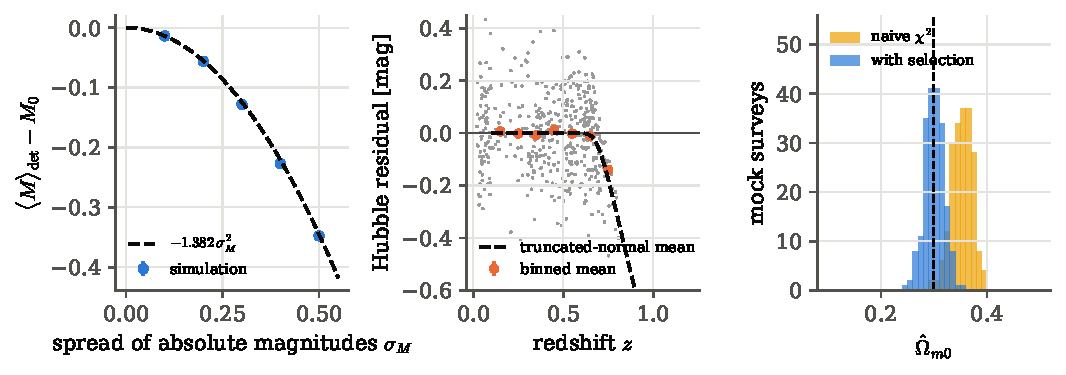
\includegraphics[width=\linewidth]{figures/chT2/malmquist.pdf}
\caption{Left: the classical Malmquist shift measured in simulation against $-1.382\sigma^2$. Middle: Hubble residuals of a magnitude-limited survey; the binned means (orange) follow the truncated-normal mean $-\sigma\phi(t)/\Phi(t)$ (dashed) and plunge as the limit cuts into the population. Right: $\Omega_{m0}$ from many mock surveys; the naive fit is biased, the likelihood with the selection term is not.}
\label{T2b:fig:malmquist}
\end{figure}

\paragraph{A relative: Eddington bias.} A related effect acts on counts rather than on luminosities. If the number of objects rises steeply towards faint fluxes, measurement noise scatters more objects up across a threshold than down, so the objects just above the threshold are, on average, fainter than they were measured. Both biases have the same cure: model the selection, and write the likelihood of the data that were actually kept.

\paragraph{Where the statistics comes back in.} The conditional density \eqref{T2b:eq:malmquist} is Bayes' theorem of \cref{ch:05}, with the luminosity function as prior and the volume factor as likelihood. The truncated likelihood is the likelihood of \cref{ch:03} written for the data actually collected. Selection functions that are known only from simulations are a Monte Carlo problem (\cref{ch:06}), and when they are folded into a hierarchical supernova model the posterior is explored by MCMC (\cref{ch:09}).
\section{Galaxies as biased tracers in redshift space}
\label{T2b:sec:tracers}

A redshift survey records, for each galaxy, two angles on the sky and a redshift. The Dark Energy Spectroscopic Instrument (DESI) did this for more than six million galaxies and quasars in its first year: bright galaxies at $0.1<z<0.4$, luminous red galaxies at $0.4<z<1.1$, star-forming emission-line galaxies at $0.8<z<1.6$, quasars at $0.8<z<2.1$, and the absorption of quasar light by intergalactic hydrogen (the Lyman-$\alpha$ forest) out to $z\approx4$ \cite[Sec.~2.2, Table~1]{DESI2024VI}. A fiducial cosmology turns each redshift into a distance and the survey into a three-dimensional map of points. The counts in cells of that map define the galaxy overdensity $\delta_g(\bm x)=n(\bm x)/\bar n-1$, and its two-point statistics, the correlation function $\xi_g(r)$ and the power spectrum $P_g(k)$ of \cref{ch:07}, are what the statistics chapters work with.

The map is not the matter field. Three things stand between them. Galaxies form only where matter has collapsed into haloes, so they are \emph{biased}: their density contrast is larger than that of the matter. Galaxies are discrete points, so their map carries \emph{shot noise}. And the redshift contains the galaxy's peculiar velocity as well as its distance, so the map is \emph{distorted} along the line of sight.

\paragraph{The question.} How is the galaxy power spectrum related to the matter power spectrum on large scales, and what is the noise of a measured $P_g$?

\subsection{Why galaxies cluster more strongly than matter}

The inputs are two. \emph{Physical:} a galaxy forms where the local density, smoothed on the scale of a halo, exceeds a threshold. \emph{Mathematical:} the initial density field is Gaussian. Write the local density at $\bm x$ as $u(\bm x)$, with variance $\sigma^2$, and say a galaxy forms where $u>\nu\sigma$; the number $\nu$ measures how rare the galaxies are. The local density is a sum of two parts, $u=u_{\rm long}+u_{\rm short}$: a long-wavelength part, shared with the surroundings over tens of megaparsecs, and a short-wavelength part that varies from halo to halo and decides locally whether the threshold is crossed. Only the first can link a galaxy to matter far away.

\emph{What we know} is that a galaxy formed at $\bm x$. \emph{What does that tell us about the matter at $\bm y$, a distance $r$ away?} The galaxy is a sign that $u(\bm x)$ was high. Because $u(\bm x)$ and $\delta(\bm y)$ are correlated, the matter at $\bm y$ is denser than average too. The cross-correlation of galaxies and matter is exactly that expected density:
\begin{align}
  \xi_{gm}(r)
  &\eqby{1}\frac{\E[I(\bm x)\,\delta(\bm y)]}{\E[I]}
  \eqby{2}\E\big[\delta(\bm y)\given u(\bm x)>\nu\sigma\big]
  \eqby{3}\E\Big[\frac{\xi(r)}{\sigma^2}\,u\;\Big|\;u>\nu\sigma\Big]
  \eqby{4}\frac{\xi(r)}{\sigma}\,\frac{\phi(\nu)}{1-\Phi(\nu)}\equiv b_L\,\xi(r) .
  \label{T2b:eq:threshold-bias}
\end{align}
\begin{explain}
  \item $I(\bm x)$ is $1$ where a galaxy forms and $0$ elsewhere, so $\delta_g=I/\E[I]-1$; the $-1$ drops out because $\E[\delta]=0$.
  \item Dividing by $\E[I]=\Prob(u>\nu\sigma)$ turns the average into a conditional expectation.
  \item For two jointly Gaussian variables the conditional mean is linear: $\E[\delta(\bm y)\given u]=\frac{\Cov(\delta(\bm y),u(\bm x))}{\Var u}\,u$ (derived in \cref{7a:eq:condmean} and \cref{2b:sec:mvn-conditional}). Which part of $u(\bm x)$ is correlated with matter a distance $r$ away? Split $u=u_{\rm long}+u_{\rm short}$ as above. The short-wavelength part varies over the size of a halo and has no memory of what happens tens of megaparsecs away, so $\Cov(\delta(\bm y),u_{\rm short}(\bm x))=0$. The long-wavelength part is the matter field itself, smoothed over a region much smaller than $r$, so $\Cov(\delta(\bm y),u_{\rm long}(\bm x))=\xi(r)$, the matter correlation. Hence $\Cov(\delta(\bm y),u(\bm x))=\xi(r)$, while $\Var u=\sigma^2$ counts both parts.
  \item The mean of a Gaussian above $\nu\sigma$ is $\sigma\phi(\nu)/[1-\Phi(\nu)]$, the upper-tail version of \eqref{T2b:eq:trunc-mean}.
\end{explain}
For rare galaxies, $\nu\gg1$, the ratio $\phi(\nu)/[1-\Phi(\nu)]\to\nu$, and $b_L\to\nu/\sigma$: the rarest objects are the most strongly clustered. This is Kaiser's explanation of why rich galaxy clusters cluster more strongly than galaxies.

\emph{From galaxy--matter to galaxy--galaxy.} \Cref{T2b:eq:threshold-bias} conditions on one galaxy and looks at the matter. The galaxy map has a galaxy at both ends of each pair, so both points are now conditioned. Write $x_1=u(\bm x)/\sigma$ and $x_2=u(\bm y)/\sigma$ for the two local densities in units of $\sigma$. They are jointly Gaussian with unit variances and a small correlation $\rho=\xi(r)/\sigma^2$ (the long-wavelength parts carry it, as in item 3). Then
\begin{align}
  1+\xi_{gg}(r)
  &\eqby{1}\frac{\E[I(\bm x)I(\bm y)]}{\E[I]^2}
  \eqby{2}\frac{1}{\E[I]^2}\int_\nu^\infty\!\!\int_\nu^\infty\phi(x_1)\phi(x_2)\big(1+\rho\,x_1x_2\big)\,\dd x_1\dd x_2\nonumber\\
  &\eqby{3}1+\rho\Big[\frac{\int_\nu^\infty x\,\phi(x)\,\dd x}{1-\Phi(\nu)}\Big]^2
  \eqby{4}1+\frac{\xi(r)}{\sigma^2}\Big[\frac{\phi(\nu)}{1-\Phi(\nu)}\Big]^2
  =1+b_L^2\,\xi(r) .
  \label{T2b:eq:threshold-auto}
\end{align}
\begin{explain}
  \item $\delta_g=I/\E[I]-1$, so $\E[(1+\delta_g(\bm x))(1+\delta_g(\bm y))]=1+\xi_{gg}$.
  \item The bivariate Gaussian density with correlation $\rho$ is $\frac{1}{2\pi\sqrt{1-\rho^2}}\exp\big[-\frac{x_1^2-2\rho x_1x_2+x_2^2}{2(1-\rho^2)}\big]$. To first order in $\rho$ the prefactor and the $1-\rho^2$ are unchanged, and the exponent gains $+\rho x_1x_2$, so the density is $\phi(x_1)\phi(x_2)e^{\rho x_1x_2}\approx\phi(x_1)\phi(x_2)(1+\rho x_1x_2)$.
  \item The $1$ integrates to $[1-\Phi(\nu)]^2=\E[I]^2$. The $\rho x_1x_2$ term factorises into two identical one-dimensional integrals.
  \item $\int_\nu^\infty x\phi(x)\dd x=[-\phi(x)]_\nu^\infty=\phi(\nu)$, as in \eqref{T2b:eq:trunc-mean}. Compare with \eqref{T2b:eq:threshold-bias}: $b_L=\phi(\nu)/\{\sigma[1-\Phi(\nu)]\}$.
\end{explain}
Each conditioned point contributes one factor $b_L$: a galaxy at $\bm x$ raises the expected density near $\bm y$ by $b_L\xi$ (that is \eqref{T2b:eq:threshold-bias}), and the threshold at $\bm y$ turns that raised density into $b_L$ times as many extra galaxies. So $\xi_{gg}=b_L^2\,\xi$, and since the power spectrum is the Fourier transform of the correlation function, $P_{gg}=b_L^2P$.

This bias is ``Lagrangian'': it describes where the galaxies formed. Afterwards they move with the matter, and the motion adds the matter's own contrast. \emph{Label each bit of matter by where it started.} Call the starting (Lagrangian) position $\bm q$. Write $\delta_L(\bm q)$ for the linear matter contrast there, grown to the time we observe with the linear growth factor, so that $b_L\delta_L$ is the galaxies' contrast of \eqref{T2b:eq:threshold-bias} at their birth place. At the start the matter is uniform to first order, while the galaxies already carry their contrast $\delta_g^L=b_L\delta_L$. \emph{Move everything.} Each bit of matter, and any galaxy riding in it, moves to its present (Eulerian) position $\bm x=\bm q+\bm\psi(\bm q)$, with $\bm\psi$ the displacement. A small volume $\dd^3q$ becomes $\dd^3x=J\,\dd^3q$, with $J=|\det(\partial x_i/\partial q_j)|$ the Jacobian of the map. \emph{Count.} No galaxy and no matter is created or lost on the way, so the number in the small volume is the same before and after:
\begin{align}
  \bar n_g\big(1+\delta_g(\bm x)\big)\,\dd^3x
  &\eqby{1}\bar n_g\big(1+b_L\delta_L(\bm q)\big)\,\dd^3q
  \;\;\Longrightarrow\;\;
  1+\delta_g\eqby{2}\frac{1+b_L\delta_L}{J},\qquad
  1+\delta\eqby{3}\frac1J,\nonumber\\
  1+\delta_g
  &\eqby{4}\big(1+b_L\delta_L\big)\big(1+\delta\big)
  \eqby{5}1+b_L\delta+\delta+O(\delta^2).
  \label{T2b:eq:lagr-to-euler}
\end{align}
\begin{explain}
  \item Number conservation for the galaxies; $\bar n_g$, the mean density, is the same before and after because the total volume and number do not change.
  \item Divide by $\bar n_g\,\dd^3x=\bar n_g J\,\dd^3q$.
  \item The same count for the matter, which started uniform.
  \item Eliminate $J$ between the two.
  \item Multiply out and keep first-order terms. To first order the evolved contrast and the linear one are the same field, $\delta=\delta_L$, and $\bm x$ and $\bm q$ differ only by the small displacement, so $\delta_L(\bm q)=\delta(\bm x)$ to this order.
\end{explain}
So, to first order,
\begin{equation}
  \delta_g=(1+b_L)\,\delta\equiv b\,\delta ,\qquad P_g(k)=b^2P(k),
  \label{T2b:eq:eulerian-bias}
\end{equation}
the ``continuity'' derivation that Cooray and Sheth mention for the large-scale bias of haloes \cite[Sec.~3.3]{CooraySheth2002}.

The halo-model version of the same idea gives each halo mass its bias, quoted in a different variable. A halo of mass $m$ forms where the linear density smoothed on the scale of that mass, of rms $\sigma(m)$, exceeds the spherical-collapse threshold $\delta_{\rm sc}\approx1.69$. In our language the threshold in units of $\sigma$ is $\nu=\delta_{\rm sc}/\sigma(m)$. Cooray and Sheth use instead its square, which we write $\nu_h\equiv\delta_{\rm sc}^2/\sigma^2(m)=\nu^2$ to keep the two apart, and quote $b_1(m)=1+(\nu_h-1)/\delta_{\rm sc}$ for spherical collapse, with an improved form fitted to simulations \cite[eqs.~(53), (68)--(70)]{CooraySheth2002}. \emph{How does this compare with ours?} The ``$1+$'' is the step from Lagrangian to Eulerian just derived. For the Lagrangian part, our high-threshold limit gives
\[
  b_L\to\frac{\nu}{\sigma}=\frac{\delta_{\rm sc}}{\sigma^2}=\frac{\nu_h}{\delta_{\rm sc}} ,
\]
so the halo formula differs from ours only by the $-1$. It comes from what is being counted. Our $b_L$ belongs to the fraction of space above a threshold, a Gaussian tail. The halo model counts haloes in a narrow mass range, which is the rate at which that tail changes with mass, and for spherical collapse this abundance goes as $\nu_h^{1/2}e^{-\nu_h/2}$ instead of a tail probability. A long-wavelength contrast $\delta_{\rm long}$ lowers the barrier to $\delta_{\rm sc}-\delta_{\rm long}$, so $\nu_h\to(\delta_{\rm sc}-\delta_{\rm long})^2/\sigma^2$ and $\dd\nu_h/\dd\delta_{\rm long}=-2\nu_h/\delta_{\rm sc}$. The fractional change of the abundance is then
\[
  \frac{\dd}{\dd\delta_{\rm long}}\Big[\tfrac12\ln\nu_h-\tfrac12\nu_h\Big]
  =\Big(\frac{1}{2\nu_h}-\frac12\Big)\Big(-\frac{2\nu_h}{\delta_{\rm sc}}\Big)
  =\frac{\nu_h-1}{\delta_{\rm sc}} ,
\]
the Lagrangian bias of the halo formula. The $\nu_h$ is our threshold effect, and the $-1$ comes from the prefactor $\nu_h^{1/2}$. For rare haloes, $\nu_h\gg1$, the two agree. A galaxy population then has the occupation-weighted average bias $b_{\rm gal}=\int\dd m\,n(m)\,b_1(m)\langle N_{\rm gal}\given m\rangle/\bar n_{\rm gal}$, and $P_{\rm gal}\approx b_{\rm gal}^2P_{\rm lin}$ on large scales \cite[eqs.~(130)--(131)]{CooraySheth2002}. Since $b_1(m)$ grows with $\nu_h$, and so with mass, luminous red galaxies, which live in massive haloes, are more strongly biased than emission-line galaxies, which live in smaller ones.

\begin{keyidea}[Linear bias]
On scales much larger than a halo, the galaxy density contrast is proportional to the matter density contrast, $\delta_g=b\,\delta$, so $P_g(k)=b^2P(k)$ and $\xi_g(r)=b^2\xi(r)$. The shape of the clustering is the matter's; only its amplitude belongs to the galaxies. The bias is a nuisance parameter in every fit of galaxy clustering.
\end{keyidea}

\subsection{Shot noise}

Galaxies are a discrete sample of a continuous field: given the field, the number of galaxies in a small cell is Poisson-distributed with mean $\bar n(1+\delta_g)\,\dd V$ (\cref{2a:sec:poisson-inputs}). What does that do to the measured power? Put $N=\bar nV$ galaxies at positions $\bm x_i$ in a box of volume $V$. The density is a sum of spikes, $n(\bm x)=\sum_i\delta_D(\bm x-\bm x_i)$, and its Fourier transform at any $\bm k\ne0$ is a sum of phases, so with the convention $\E[\delta_{\bm k}\delta^*_{\bm k}]=VP(k)$ of \cref{11a:sec:shot},
\begin{align}
  \hat P_g(k)=\frac{|\delta_{g,\bm k}|^2}{V}
  &\eqby{1}\frac{1}{V\bar n^2}\sum_i\sum_je^{-i\bm k\cdot(\bm x_i-\bm x_j)}
  \eqby{2}\frac{1}{V\bar n^2}\Big[N+\sum_{i\ne j}e^{-i\bm k\cdot(\bm x_i-\bm x_j)}\Big],\nonumber\\
  \langle\hat P_g(k)\rangle
  &\eqby{3}\frac{N}{V\bar n^2}+b^2P(k)
  \eqby{4}b^2P(k)+\frac1{\bar n}.
  \label{T2b:eq:shot}
\end{align}
\begin{explain}
  \item $\delta_g=n/\bar n-1$, and the $-1$ only touches $\bm k=0$, so $\delta_{g,\bm k}=\bar n^{-1}\sum_ie^{-i\bm k\cdot\bm x_i}$; the modulus squared is a double sum.
  \item Split off the $i=j$ terms: each is $e^0=1$, and there are $N$ of them.
  \item The pairs of different galaxies are the clustering: averaged over realisations, their phases add up to $V\bar n^2\,b^2P(k)$, the power of the field the galaxies trace.
  \item $N=\bar nV$.
\end{explain}
The self-pairs, each galaxy paired with itself, add a constant $1/\bar n$ at every $k$: a white-noise floor, the \newterm{shot noise} (derived in full in \cref{11a:sec:shot}).

How noisy is the measured $\hat P_g$? The Gaussian-field result of \cref{ch:07} answers it in two steps. \emph{Count the modes.} In a box of volume $V$ the allowed wavevectors sit on a grid, one per $(2\pi)^3/V$ of $\bm k$-space. A shell of radius $k$ and width $\Delta k$ has volume $4\pi k^2\Delta k$, so it holds $N_k=4\pi k^2\Delta k\,V/(2\pi)^3=Vk^2\Delta k/(2\pi^2)$ grid points. The field is real, so $\delta_{-\bm k}=\delta_{\bm k}^*$ and only $N_k/2$ of them are independent. \emph{The error of one shell.} One independent mode gives $|\delta_{\bm k}|^2/V$, whose standard deviation equals its mean (it is $\frac12\chi^2_2$ times the mean, \eqref{7a:eq:mode-exp}), and the mean is now the total power $b^2P+1/\bar n$. Averaging $N_k/2$ independent modes divides the variance by $N_k/2$ (\eqref{7a:eq:var-phat}), so $\sigma_P=\sqrt{2/N_k}\,(b^2P+1/\bar n)$. Divide by the signal $b^2P$:
\begin{equation}
  \frac{\sigma_{P}}{b^2P}=\sqrt{\frac{2}{N_k}}\Big(1+\frac{1}{\bar nb^2P}\Big).
  \label{T2b:eq:pk-error}
\end{equation}
Two terms limit a survey. Cosmic variance, the $\sqrt{2/N_k}$, falls only with volume. Shot noise is negligible once $\bar nb^2P\gtrsim1$. A survey designer therefore covers as much volume as possible with just enough galaxies to reach $\bar nP\approx1$ on the scales of interest, around $k=0.1\,h$\,Mpc$^{-1}$ \cite[Sec.~4.4.5]{Weinberg2013}. DESI's ``effective volume'' $V_{\rm eff}=\int[\bar nP/(1+\bar nP)]^2\dd V$ is this trade-off in one number \cite[Table~1]{DESI2024VI}.

If several galaxies share one halo, their pairs add a second constant on large scales, the one-halo term $\int\dd m\,n(m)\langle N(N-1)\given m\rangle/\bar n^2$ \cite[eq.~(128)]{CooraySheth2002}. It behaves like extra shot noise.

\subsection{Redshift-space distortions}

The redshift of a galaxy measures its distance plus its peculiar velocity along the line of sight. In comoving coordinates the map position is $\bm s=\bm x+u_z\hat{\bm z}$, with $\hat{\bm z}$ the line of sight and $u_z=v_z/(aH)$ the velocity expressed as a distance. Galaxies falling towards an overdensity from in front are pushed back, those behind are pulled forward, and the structure looks squashed along the line of sight (\cref{T2b:fig:kaiser-cartoon}).

How strong is the squashing? The inputs are: linear theory ($|\delta|\ll1$); a distant observer, so the line of sight is the same direction $\hat{\bm z}$ for every galaxy; and velocities set by the growth of structure. That last input needs a short derivation, because the velocity is what moves the galaxies in the map.

\emph{The velocities from the growth of structure.} Matter that flows out of a region lowers its density. In comoving coordinates, with $\bm v$ the peculiar velocity, mass conservation to first order in $\delta$ and $\bm v$ reads
\begin{align}
  \frac{\partial\delta}{\partial t}
  &\eqby{1}-\frac1a\,\nabla\cdot\bm v,
  \qquad
  \frac{\partial\delta}{\partial t}\eqby{2}fH\,\delta
  \quad\Longrightarrow\quad
  \nabla\cdot\bm v\eqby{3}-afH\,\delta,
  \qquad
  \nabla\cdot\bm u\eqby{4}-f\,\delta .
  \label{T2b:eq:continuity}
\end{align}
\begin{explain}
  \item The continuity equation: the outflow rate through the surface of a small comoving volume, per unit volume, is $\nabla\cdot\bm v$ in physical units, and a comoving gradient is $a$ times a physical one, hence the $1/a$.
  \item Linear growth: $\delta(\bm x,t)=\delta(\bm x,t_0)D(t)$, with $D$ the linear growth factor, so $\partial\delta/\partial t=(\dot D/D)\delta=(\dd\ln D/\dd\ln a)(\dot a/a)\delta=fH\delta$, which defines the growth rate $f=\dd\ln D/\dd\ln a\approx\Omega_m(z)^{0.55}$.
  \item Equate the two and multiply by $-a$.
  \item Divide by $aH$: $\bm u=\bm v/(aH)$ is the velocity expressed as a comoving distance.
\end{explain}
In physical coordinates, with $\bm r=a\bm x$, the first relation is $\dot\delta=-\nabla_{\bm r}\cdot\bm v$, the form used for the local void in \cref{T2b:sec:ladder}. The divergence fixes only part of $\bm u$. In linear theory any rotation of the flow decays as the universe expands, so the flow is a gradient, $\bm u=\nabla\Phi_u$, and in Fourier space $\bm u_{\bm k}=i\bm k\,\Phi_{u,\bm k}$ points along $\bm k$. Its divergence is $i\bm k\cdot\bm u_{\bm k}=-k^2\Phi_{u,\bm k}$, and setting this equal to $-f\delta_{\bm k}$ gives $\Phi_{u,\bm k}=f\delta_{\bm k}/k^2$, so
\[
  \bm u_{\bm k}=\frac{i\bm k\,f\,\delta_{\bm k}}{k^2}.
\]

\emph{Now the map.} Galaxies are conserved by the mapping from real to redshift space, $(1+\delta_s)\,\dd^3s=(1+\delta_g)\,\dd^3x$. So
\begin{align}
  \delta_s
  &\eqby{1}\delta_g-\frac{\partial u_z}{\partial z}
  \;\;\xrightarrow{\;\text{Fourier}\;}\;\;
  \delta_{s,\bm k}\eqby{2}b\,\delta_{\bm k}-ik_z\,\frac{ik_zf}{k^2}\,\delta_{\bm k}
  \eqby{3}\big(b+f\mu^2\big)\,\delta_{\bm k},\nonumber\\
  P_s(k,\mu)
  &\eqby{4}b^2\big(1+\beta\mu^2\big)^2P(k),\qquad\beta\equiv\frac fb,\qquad\mu\equiv\frac{k_z}{k}.
  \label{T2b:eq:kaiser}
\end{align}
\begin{explain}
  \item $\dd^3s=(1+\partial u_z/\partial z)\,\dd^3x$, because only the $z$ coordinate is moved; expand to first order.
  \item $\delta_g=b\delta$, and $\partial/\partial z\to ik_z$.
  \item $-i\cdot i=1$ and $k_z^2/k^2=\mu^2$, the squared cosine of the angle between $\bm k$ and the line of sight.
  \item Square the modulus and average over realisations.
\end{explain}
This is the \newterm{Kaiser formula} \cite{Kaiser1987}. Waves across the line of sight ($\mu=0$) are untouched; waves along it are enhanced by $(1+\beta)^2$. Averaging over all directions gives the \newterm{monopole}. Directions are spread uniformly in $\mu$ between $-1$ and $1$, and the factor is even in $\mu$, so the average is $\int_0^1\dd\mu$. Expand the square and integrate term by term, with $\int_0^1\mu^2\dd\mu=\frac13$ and $\int_0^1\mu^4\dd\mu=\frac15$:
\[
  \int_0^1\big(1+\beta\mu^2\big)^2\dd\mu=\int_0^1\big(1+2\beta\mu^2+\beta^2\mu^4\big)\dd\mu=1+\frac23\beta+\frac15\beta^2 .
\]
\emph{Why this separates growth from bias.} The amplitude of $P$ is usually written through $\sigma_8$ \unpack{the rms matter contrast in spheres of $8\,h^{-1}$Mpc}, so that $P(k)/\sigma_8^2$ is a fixed shape. Write \eqref{T2b:eq:kaiser} in that form, using $b(1+\beta\mu^2)=b+f\mu^2$:
\[
  P_s(k,\mu)=\big(b\sigma_8+f\sigma_8\,\mu^2\big)^2\,\frac{P(k)}{\sigma_8^2}.
\]
The part of the amplitude that does not depend on direction is $b\sigma_8$; the part that grows as $\mu^2$ is $f\sigma_8$. Fitting how the power changes with $\mu$ gives the two separately: the angular dependence of the galaxy power spectrum measures the growth rate of structure, independently of the unknown bias. On small scales the random velocities inside haloes do the opposite and stretch groups into ``fingers'' pointing at the observer; that regime needs models beyond linear theory.

\begin{figure}[htbp]
\centering
\begin{tikzpicture}[scale=1.0]
  \begin{scope}
    \fill[formblue!12] (0,0) circle (1.3);
    \draw[form] (0,0) circle (1.3);
    \fill[formblue!45] (0,0) circle (0.25);
    \foreach \a in {90,270,0,180,45,135,225,315}
      \draw[vec] ({1.75*cos(\a)},{1.75*sin(\a)}) -- ({1.38*cos(\a)},{1.38*sin(\a)});
    \node[lbl] at (0,-2.25) {real space};
  \end{scope}
  \begin{scope}[xshift=5.2cm]
    \fill[formblue!12] (0,0) ellipse (1.3 and 0.75);
    \draw[form] (0,0) ellipse (1.3 and 0.75);
    \fill[formblue!45] (0,0) circle (0.25);
    \draw[faint,dashed] (0,0) circle (1.3);
    \node[lbl] at (0,-2.25) {redshift space};
  \end{scope}
  \draw[->,thick,softgray] (9.0,-1.6) -- (9.0,1.6);
  \node[lbl,text=softgray,align=center,anchor=west] at (9.15,0) {line of\\ sight};
  \node[lbl,align=center,anchor=north] at (9.0,-1.7) {observer\\ below};
\end{tikzpicture}
\caption{The Kaiser effect. Left: a spherical shell of galaxies around an overdensity, falling inwards (green arrows). Right: the same shell placed at the distances inferred from redshifts. Galaxies on the near side move away from us and appear farther; those on the far side move towards us and appear nearer. The shell is flattened along the line of sight; across it nothing changes (the dashed circle is the true shell).}
\label{T2b:fig:kaiser-cartoon}
\end{figure}

\subsection{The experiment: thresholds, bias and squashing in a box}

\pyname{09_tracers_rsd.py} tests \eqref{T2b:eq:threshold-bias}, \eqref{T2b:eq:eulerian-bias} and \eqref{T2b:eq:kaiser} on a simulated universe. The ingredients:
\begin{center}
\small
\begin{tabular}{@{}lll@{}}
\toprule
ingredient & value & what it stands for\\
\midrule
box side, grid & $\TwtL\,h^{-1}$Mpc, $\TwtN^3$ cells & a survey volume, periodic\\
matter field & Gaussian, linear CAMB $P(k)$ at $z=\TwtZ$ & the initial density, grown linearly\\
smoothing scale $R$ & $\TwtR\,h^{-1}$Mpc, $\sigma_R=\TwtSigR$ & the size of a halo: $u_{\rm long}$\\
small-scale part & independent, rms $\TwtSigSmall$ & unresolved physics inside haloes: $u_{\rm short}$\\
total rms $\sigma$ & $\TwtSigT$ & $\sigma^2=\sigma_R^2+\TwtSigSmall^2$\\
threshold & cells with $u>\nu\sigma$ & where galaxies form\\
growth rate & $f=\TwtF$ at $z=1$ & sets the velocities\\
\bottomrule
\end{tabular}
\end{center}
One sentence per ingredient. The box cannot resolve haloes, so the local density that decides where galaxies form is built by hand from the two parts of $u$: the field smoothed on the scale of a halo is $u_{\rm long}$, the part that correlates with distant matter; the independent small-scale part is $u_{\rm short}$, which by construction correlates with nothing. Cells above the threshold host galaxies. Then every particle and every galaxy is moved by its Zel'dovich displacement $\bm\psi_{\bm k}=i\bm k\delta_{\bm k}/k^2$, the first-order displacement of \eqref{T2b:eq:lagr-to-euler} (it has $-\nabla\cdot\bm\psi=\delta$, so $1/J=1+\delta$ to first order), and in redshift space by an extra $f\psi_z\hat{\bm z}$, which is the $u_z$ of \eqref{T2b:eq:continuity}.

\emph{Measuring $b$ without cosmic variance.} The box has only about a thousand independent modes at $k<\TwtKmax\,h$\,Mpc$^{-1}$, and in each of them the auto spectrum $|\delta_{g,\bm k}|^2$ scatters as much as its mean (\eqref{7a:eq:mode-exp}). But the box also holds the matter field that made it, and for each mode $\delta_{g,\bm k}=b\,\delta_{\bm k}+\text{noise}$. Then
\[
  \frac{\mathrm{Re}\big(\delta_{g,\bm k}\delta^*_{\bm k}\big)}{|\delta_{\bm k}|^2}=b+\frac{\mathrm{Re}(\text{noise}\cdot\delta^*_{\bm k})}{|\delta_{\bm k}|^2} ,
\]
and the random amplitude $|\delta_{\bm k}|^2$ of the particular mode cancels in the first term. The ratio is $b$ in every mode, whatever the realisation drew. The script averages it over $k<\TwtKmax\,h$\,Mpc$^{-1}$.

\Cref{T2b:fig:tracers} shows what came out. Before the move, the measured bias follows $b_L$ of \eqref{T2b:eq:threshold-bias}: $\TwtBLmOne\pm\TwtBLerrOne$ against $\TwtBLthOne$ at $\nu=1$, and $\TwtBLmTwo\pm\TwtBLerrTwo$ against $\TwtBLthTwo$ at $\nu=2$. The high-$\nu$ limit $\nu/\sigma$ ($\TwtNuHighTwo$ at $\nu=2$) is still poor at these thresholds. After the move the bias is $\TwtBEmTwo\pm\TwtBEerrTwo$ at $\nu=2$, against $1+b_L=\TwtBEthTwo$: the matter's own clustering has been added, as \eqref{T2b:eq:eulerian-bias} says.

A galaxy sample with $\nu=\TwtNuG$ and $\bar n=\TwtNbar\,h^3$Mpc$^{-3}$ ($\TwtNgal$ galaxies) has $b=\TwtBG\pm\TwtBGerr$ from the cross spectrum ($\TwtBGth$ predicted). Its auto spectrum shows the noise terms of \eqref{T2b:eq:shot}. Subtracting only the Poisson term $1/\bar n=\TwtShot\,h^{-3}$Mpc$^3$ gives an apparent bias of $\TwtBGautoNaive$, too high. \emph{What is missing?} Galaxies are placed in the selected cells as a Poisson number $N$ with mean $\lambda=\TwtLam$ per cell, so a cell often holds two or more, and its galaxies pair with one another. Those pairs are at zero separation, like the self-pairs of \eqref{T2b:eq:shot}, so they too add a constant to the power. Counting them is one line. A Poisson number has $\E N=\Var N=\lambda$, so $\E[N(N-1)]=\E N^2-\E N=(\lambda+\lambda^2)-\lambda=\lambda^2$. There are $N_{\rm sel}=\bar nV/\lambda$ selected cells, so the number of within-cell pairs is $N_{\rm sel}\lambda^2=\bar nV\lambda$, and in the same normalisation as the $N/(V\bar n^2)$ of \eqref{T2b:eq:shot},
\[
  \text{one-halo constant}=\frac{N_{\rm sel}\,\E[N(N-1)]}{V\bar n^2}=\frac{\bar nV\lambda}{V\bar n^2}=\frac{\lambda}{\bar n}=\TwtLam\times\TwtShot\approx\TwtOneHalo\,h^{-3}\text{Mpc}^3 ,
\]
the cell version of the one-halo term above. Subtracting it too gives $\TwtBGauto$, in agreement with the cross spectrum. In redshift space the ratio $P_s(k,\mu)/P_r(k)$ rises with $\mu$ as $(1+\beta\mu^2)^2$ with $\beta=f/b=\TwtBeta$; the monopole ratio is $\TwtMono$ against $1+\frac23\beta+\frac15\beta^2=\TwtMonoTh$. The highest-$\mu$ bin, which holds the fewest modes, scatters most. For the matter ($b=1$) one box is not enough to read that bin, so the script repeats the matter part on fresh boxes. Averaged over $\TwtNbox$ boxes, the enhancement at $\mu\approx0.95$ is $\TwtRatioMParMean\pm\TwtRatioMParErr$ against $\TwtRatioMParTh$: the Zel'dovich motions have begun to smear the largest line-of-sight displacements, the first sign of the non-linear regime.

\begin{figure}[htbp]
\centering
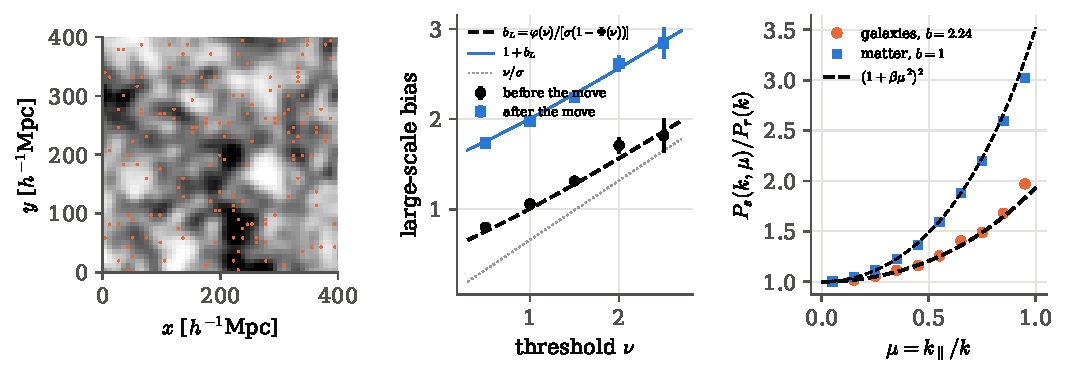
\includegraphics[width=\linewidth]{figures/chT2/tracers_rsd.pdf}
\caption{Left: a slice of the smoothed density field with the galaxies of one thin slab (orange); the galaxies sit in the dense regions. Middle: the large-scale bias against the threshold $\nu$; before the move it follows $b_L$ (dashed), after it $1+b_L$ (blue line); the dotted line is the high-threshold limit $\nu/\sigma$. Right: redshift-space power divided by real-space power, against $\mu$; galaxies (orange) and matter (blue) follow the Kaiser factor with $\beta=f/b$ and $\beta=f$ respectively.}
\label{T2b:fig:tracers}
\end{figure}

\paragraph{Nerfed, honestly.} The box is a single Gaussian realisation of $(1\,h^{-1}{\rm Gpc})^3$ with $7.8\,h^{-1}$Mpc cells, run in seconds, and the haloes are replaced by a threshold on a field with a white-noise small-scale part. Research analyses use $N$-body simulations with $10^{10}$ particles, find haloes in them, populate the haloes with galaxies by an occupation model fitted to the small-scale clustering, and build hundreds to thousands of approximate mock catalogues to estimate the covariance of $\hat P_g$.

\paragraph{Where the statistics comes back in.} The galaxy power spectrum and correlation function, their estimators and their Gaussian covariance, are the random-field statistics of \cref{ch:07}. Shot noise is the Poisson process of \cref{ch:02}. Bias, the shot-noise amplitude and $f\sigma_8$ are the parameters of a clustering likelihood whose forecast is a Fisher calculation (\cref{ch:10}) and whose posterior is sampled with MCMC (\cref{ch:09}). Galaxy clustering, redshift-space distortions and peculiar velocities as cosmological data are the subject of \cref{ch:11}.
\section{Baryon acoustic oscillations: a standard ruler}
\label{T2b:sec:bao}

Before recombination, photons and baryons were held together by Thomson scattering into a single hot fluid. Every small overdensity in that fluid launched a spherical sound wave, which ran outwards until the baryons were released from the photons and then stopped. How fast did it run? \emph{The pressure comes from the photons, the inertia from both.} Radiation has pressure $p=\rho_\gamma c^2/3$; the baryons add mass but, being cold, no pressure. A sound wave squeezes photons and baryons together, so both number densities rise by the same fraction. For photons $\rho_\gamma\propto T^4$ and $n_\gamma\propto T^3$, so $\delta\rho_\gamma/\rho_\gamma=\frac43\,\delta n/n$; for baryons $\delta\rho_b/\rho_b=\delta n/n$. Hence $\delta\rho_b=\frac34(\rho_b/\rho_\gamma)\,\delta\rho_\gamma$, and
\[
  c_s^2=\frac{\delta p}{\delta\rho}
  =\frac{c^2\,\delta\rho_\gamma/3}{\delta\rho_\gamma+\delta\rho_b}
  =\frac{c^2}{3(1+R)},\qquad R\equiv\frac{3\rho_b}{4\rho_\gamma}.
\]
Without baryons this is $c/\sqrt3$; the baryons' inertia slows the wave a little. \emph{How far did it get?} In a time $\dd t$ the wave covers a physical distance $c_s\dd t$, which is a comoving distance $c_s\dd t/a$. With $a=1/(1+z)$ and $\dd z/\dd t=-(1+z)H$, this is $c_s\dd t/a=-c_s\,\dd z/H$. Summing from the beginning ($z=\infty$) to the moment the baryons stop feeling the photons' push, the \newterm{drag epoch} $z_d\approx1060$ (slightly after recombination, because photons outnumber baryons by about a billion to one and keep dragging them a little longer), each initial peak was left with a thin shell of extra baryons at the comoving distance sound had travelled,
\begin{equation}
  r_d=\int_{z_d}^{\infty}\frac{c_s(z)}{H(z)}\,\dd z\approx147\ \text{Mpc}
  \label{T2b:eq:rd}
\end{equation}
\cite[eqs.~(2.3)--(2.4)]{DESI2024VI}. Dark matter fell into both the central peak and the shell, and galaxies later formed in both. So each overdensity is surrounded by a shell at $r_d$, and pairs of galaxies separated by $r_d$, one in a peak and one in its shell, are slightly more common than chance. Counting pairs by separation, that excess shows up as a bump in the correlation function at $r\approx r_d$, the feature computed in \cref{ch:T1}. The integral \eqref{T2b:eq:rd} depends only on the physical matter and baryon densities $\omega_m=\Omega_mh^2$ and $\omega_b=\Omega_bh^2$ (through $H$ and $R$) and the number of relativistic species $N_{\rm eff}$ (through $H$). A fit to its numerical value, quoted by DESI, is $r_d\approx147.05\,(\omega_m/0.1432)^{-0.23}(N_{\rm eff}/3.04)^{-0.1}(\omega_b/0.02236)^{-0.13}$\,Mpc \cite[eq.~(2.5)]{DESI2024VI}; the exponents are fitted numbers, not derived ones. The CMB measures it to $0.2\%$: $r_d=147.09\pm0.26$\,Mpc \cite[Table~2]{Planck2018VI}. A feature of known length, seen at many redshifts, is a \newterm{standard ruler}.

\paragraph{The question.} What exactly does the position of the bump measure, how is it extracted from a noisy correlation function, how precisely, and what did DESI find?

\subsection{What the ruler measures}

The survey measures angles and redshifts, not lengths. A pair of galaxies at redshift $z$ separated by $r_d$ \emph{across} the line of sight subtends an angle
\[
  \Delta\theta=\frac{r_d}{D_M(z)},\qquad D_M(z)=\int_0^z\frac{c\,\dd z'}{H(z')}\ \ \text{(flat)},
\]
where $D_M$ is the transverse comoving distance \cite[eq.~(16)]{Hogg1999}. A pair separated by $r_d$ \emph{along} the line of sight differs in redshift by $\Delta z$, and since the comoving distance changes by $\dd\chi=c\,\dd z/H(z)$,
\[
  \Delta z=\frac{r_d}{D_H(z)},\qquad D_H(z)\equiv\frac{c}{H(z)} .
\]
So the bump measures $D_M/r_d$ from its angular size and $D_H/r_d$ from its depth in redshift \cite[Sec.~2.1]{DESI2024VI}. \Cref{T2b:fig:bao-geometry} draws both.

\begin{figure}[htbp]
\centering
\begin{tikzpicture}[scale=1.0]
  \fill (0,0) circle (1.6pt) node[below,lbl] {observer};
  \draw[faint] (0,0) -- (8.6,1.55);
  \draw[faint] (0,0) -- (8.6,-1.55);
  \coordinate (A) at (7.2,1.3); \coordinate (B) at (7.2,-1.3);
  \fill[formblue] (A) circle (2.2pt); \fill[formblue] (B) circle (2.2pt);
  \draw[form,dashed] (A) -- (B);
  \node[lbl,anchor=west,text=formblue] at (7.35,0.25) {$r_d$ across};
  \draw[bdry,thin] (2.2,0.397) arc (10.2:-10.2:2.24);
  \node[lbl,anchor=west,text=bdryred] at (2.35,0) {$\Delta\theta=r_d/D_M$};
  \draw[decorate,decoration={brace,amplitude=4pt,mirror}] (0,-0.45) -- (7.2,-1.75) node[midway,below=4pt,lbl] {$D_M(z)$};
  \begin{scope}[xshift=0cm]
    \fill[fibreorange] (9.6,0) circle (2.2pt); \fill[fibreorange] (12.2,0) circle (2.2pt);
    \draw[fibre,dashed] (9.6,0) -- (12.2,0);
    \node[lbl,text=fibreorange] at (10.9,0.35) {$r_d$ along};
    \node[lbl,text=fibreorange,align=center] at (10.9,-0.75) {$\Delta z=r_d/D_H$\\ $D_H=c/H(z)$};
  \end{scope}
\end{tikzpicture}
\caption{What a standard ruler measures. Left: two galaxies separated by $r_d$ across the line of sight appear an angle $\Delta\theta=r_d/D_M$ apart. Right: two galaxies separated by $r_d$ along the line of sight differ in redshift by $\Delta z=r_d/D_H$. The first gives the distance, the second the expansion rate, both in units of $r_d$.}
\label{T2b:fig:bao-geometry}
\end{figure}

\paragraph{The map is drawn with an assumed cosmology.} To place galaxies in space at all, the survey assumes a fiducial cosmology, with distances $D_M^{\rm fid}$ and $D_H^{\rm fid}$ and a sound horizon $r_d^{\rm fid}$. The question, in words: \emph{if the true distances differ from the assumed ones, where in the fiducial map does the true ring of radius $r_d$ end up, and how do we read the true distances off its position?}

\emph{Across the line of sight first.} The survey turns a measured angle into a length with the assumed distance, and the angle is set by the true one:
\begin{align}
  r_\perp^{\rm app}
  &\eqby{1}D_M^{\rm fid}\,\Delta\theta
  \eqby{2}r_d\,\frac{D_M^{\rm fid}}{D_M}
  \eqby{3}\frac{r_d^{\rm fid}}{\alpha_\perp},
  \qquad
  \alpha_\perp\equiv\frac{D_M/r_d}{D_M^{\rm fid}/r_d^{\rm fid}} .
  \label{T2b:eq:rperp-app}
\end{align}
\begin{explain}
  \item The map converts angle to transverse length with the fiducial distance.
  \item The true pair at separation $r_d$ subtends $\Delta\theta=r_d/D_M$, with the true $D_M$.
  \item Name the ratio of the apparent ring to the ring the template expects, $r_\perp^{\rm app}/r_d^{\rm fid}=1/\alpha_\perp$.
\end{explain}
\emph{Along the line of sight, the same way.} A redshift difference becomes a length through the fiducial $D_H$, and the true one sets $\Delta z=r_d/D_H$: $r_\parallel^{\rm app}=D_H^{\rm fid}\Delta z=r_dD_H^{\rm fid}/D_H=r_d^{\rm fid}/\alpha_\parallel$. Together,
\begin{equation}
  \alpha_\perp=\frac{D_M/r_d}{D_M^{\rm fid}/r_d^{\rm fid}},\qquad
  \alpha_\parallel=\frac{D_H/r_d}{D_H^{\rm fid}/r_d^{\rm fid}} .
  \label{T2b:eq:alphas}
\end{equation}
So a sphere of radius $r_d$ in the true universe appears in the fiducial map as an ellipsoid with semi-axes $r_d^{\rm fid}/\alpha_\perp$ across the line of sight and $r_d^{\rm fid}/\alpha_\parallel$ along it. Read the direction carefully: $\alpha>1$ means the true distance (in units of $r_d$) is larger than assumed, the ring looks \emph{smaller} than the template, and the feature appears at smaller $r$.

\emph{From the ring to the template fit.} The template correlation function $\xi_{\rm fid}(r)$ of the fiducial cosmology has its bump at $r=r_d^{\rm fid}$. The data have it at $r^{\rm app}=r_d^{\rm fid}/\alpha$. The dilated template $\xi_{\rm fid}(\alpha r)$ has its bump where $\alpha r=r_d^{\rm fid}$, that is at $r=r_d^{\rm fid}/\alpha$, exactly where the data put it. So fitting the data with $\xi_{\rm fid}(\alpha r)$ and finding the best $\alpha$ measures the ratio of true to fiducial distance in \eqref{T2b:eq:alphas}. DESI reports the same information in the form $D_M/r_d$ and $D_H/r_d$ \cite[Sec.~2.1]{DESI2024VI}, which is our $\alpha_\perp$ and $\alpha_\parallel$ multiplied by the fiducial $D_M^{\rm fid}/r_d^{\rm fid}$ and $D_H^{\rm fid}/r_d^{\rm fid}$.

\paragraph{Why $D_V$, and why the factor $z$.} When the data are too noisy to separate the two directions, one fits the angle-averaged correlation function with a single dilation $\alpha$. The single scale that preserves the volume of the ellipsoid, which is what an angle average responds to at first order, is the geometric mean of its three axes:
\begin{align}
  \alpha_{\rm iso}
  &\eqby{1}\big(\alpha_\perp^2\,\alpha_\parallel\big)^{1/3}
  \eqby{2}\frac{\big(D_M^2D_H\big)^{1/3}/r_d}{\big(D_M^{{\rm fid}\,2}D_H^{\rm fid}\big)^{1/3}/r_d^{\rm fid}}
  \eqby{3}\frac{D_V/r_d}{D_V^{\rm fid}/r_d^{\rm fid}},\qquad
  D_V\equiv\big(z\,D_M^2\,D_H\big)^{1/3}.
  \label{T2b:eq:dv}
\end{align}
\begin{explain}
  \item Two transverse axes and one radial axis: the volume scales as $\alpha_\perp^2\alpha_\parallel$.
  \item Substitute \eqref{T2b:eq:alphas}.
  \item Multiply numerator and denominator by $z^{1/3}$, which cancels.
\end{explain}
The factor $z$ is a convention, and it is there so that $D_V$ is a distance with a familiar limit: at low redshift $D_M\approx cz/H_0$ and $D_H\approx c/H_0$, so $D_V\approx\big(z\cdot(cz/H_0)^2\cdot c/H_0\big)^{1/3}=cz/H_0$, the Hubble-law distance. This is Eisenstein et al.'s eq.~(2), $D_V=[D_M^2\,cz/H(z)]^{1/3}$ \cite[Sec.~4]{Eisenstein2005}, and DESI's eq.~(2.6) \cite{DESI2024VI}.

\begin{pitfall}[Which ``angular diameter distance''?]
Three conventions meet here. Hogg's $D_A=D_M/(1+z)$ is the physical angular diameter distance \cite[eq.~(18)]{Hogg1999}, and so is the $D_A$ of \cref{ch:T1}. Weinberg et al.\ write $D_A$ for the \emph{comoving} angular diameter distance, which is $D_M$ \cite[p.~46]{Weinberg2013}. Eisenstein et al.\ and DESI write $D_M$. A factor $(1+z)$ in a BAO formula is usually this.
\end{pitfall}

\subsection{Measuring the dilation, and how well}

A correlation function is measured in bins of separation $r_i$. How noisy is each bin, and how are neighbouring bins tied together? For a Gaussian field the answer follows from the power spectrum. The correlation function is the Fourier transform of the power, so the estimate in bin $i$ is a weighted sum of the power measured in thin $k$-shells, $\hat\xi(r_i)=\sum_{\rm shells}\frac{k^2\Delta k}{2\pi^2}\hat P(k)\,\bar j_0(kr_i)$, where $\bar j_0$ is the spherical Bessel function $\sin x/x$ averaged over the width of the bin (\cref{7a:sec:wk}). Different shells are independent, and each has $\Var\hat P=2P_{\rm tot}^2/N_k$ with $P_{\rm tot}=b^2P+1/\bar n$ and $N_k=Vk^2\Delta k/(2\pi^2)$ modes (\eqref{T2b:eq:pk-error}). So
\begin{align}
  \Cov\big[\hat\xi(r_i),\hat\xi(r_j)\big]
  &\eqby{1}\sum_{\rm shells}\Big(\frac{k^2\Delta k}{2\pi^2}\Big)^2\bar j_0(kr_i)\,\bar j_0(kr_j)\,\frac{2P_{\rm tot}^2}{Vk^2\Delta k/(2\pi^2)}\nonumber\\
  &\eqby{2}\frac{2}{V}\int\frac{k^2\dd k}{2\pi^2}\Big[b^2P(k)+\frac1{\bar n}\Big]^2\bar j_0(kr_i)\,\bar j_0(kr_j).
  \label{T2b:eq:xi-cov}
\end{align}
\begin{explain}
  \item The covariance of two weighted sums of independent terms is the sum of weight times weight times variance.
  \item Cancel one factor $k^2\Delta k/(2\pi^2)$ and let the shells become thin.
\end{explain}
Each piece now has a meaning. The $1/V$ is the averaging over independent modes: a bigger survey has more of them. The square is there because a variance of a power is the square of the power (one mode's $|\delta_{\bm k}|^2$ scatters as much as its mean). The $1/\bar n$ inside it is the shot noise of \eqref{T2b:eq:shot}. And since every bin draws on the same shells, neighbouring bins share their errors.

The model is the fiducial template, dilated, plus a smooth curve that absorbs everything the BAO feature does not determine \cite[p.~9]{DESI2024VI}:
\begin{equation}
  \xi_{\rm model}(r)=B^2\,\xi_{\rm fid}(\alpha r)+a_0+\frac{a_1}{r}+\frac{a_2}{r^2}.
  \label{T2b:eq:bao-model}
\end{equation}
Each term has one job. $\alpha$ is the dilation of \eqref{T2b:eq:alphas}, the only number we want. $B^2$ absorbs the amplitude: the galaxy bias $b^2$ of \cref{T2b:sec:tracers} relative to the template's, and the redshift-space boost. $a_0$, $a_1/r$ and $a_2/r^2$ absorb the broadband shape, whatever smooth errors the template has from non-linear growth or a bias that changes slowly with scale. None of them can make a narrow bump, so the bump's position, and with it $\alpha$, is left to the data.

\emph{Solving for the nuisance terms.} For a fixed trial $\alpha$ the model is a fixed matrix $X$ (its four columns are $\xi_{\rm fid}(\alpha r_i)$, $1$, $1/r_i$, $1/r_i^2$) times the vector $\bm\beta=(B^2,a_0,a_1,a_2)$. So $\chi^2(\bm\beta)=(\hat{\bm\xi}-X\bm\beta)\T\Cmat^{-1}(\hat{\bm\xi}-X\bm\beta)$ is quadratic in $\bm\beta$, and a quadratic has one minimum, found exactly by generalised least squares (\cref{ch:03}), $\hat{\bm\beta}=(X\T\Cmat^{-1}X)^{-1}X\T\Cmat^{-1}\hat{\bm\xi}$. Marginalising $\bm\beta$ with flat priors instead (\cref{ch:05}) integrates $e^{-\chi^2/2}$ over a Gaussian in $\bm\beta$, which gives $e^{-\chi^2_{\min}/2}$ times $\det(X\T\Cmat^{-1}X)^{-1/2}$, the same structure as the amplitude integral of \eqref{T2b:eq:photoz-like}; that factor changes only slowly with $\alpha$, so the two routes agree closely. What is left is a profile $\chi^2(\alpha)$.

\emph{Is the bump really there?} The \newterm{BAO detection significance} compares the profile with the best fit of a template with the wiggles removed: $\Delta\chi^2=\chi^2_{\rm no\,wiggle}-\chi^2_{\rm BAO}$. The null hypothesis is the smooth, wiggle-free correlation function, and the test asks: if there were no bump, would a $\Delta\chi^2$ this large, or larger, be something we would reasonably expect from noise? Think of the BAO model as the no-wiggle model plus the wiggles with a free amplitude; the null sets that one amplitude to zero. Then Wilks' theorem (\cref{4a:sec:wilks}, \eqref{4a:eq:delta-chi2}) says that under the null $\Delta\chi^2$ is a $\chi^2$ with one degree of freedom, which is the square of one unit Gaussian $Z$. So
\[
  \Prob\big(\Delta\chi^2>n^2\given\text{no bump}\big)=\Prob(|Z|>n)=2\big[1-\Phi(n)\big],
\]
the probability of a Gaussian fluctuation beyond $n$ standard deviations. A measured $\Delta\chi^2$ therefore corresponds to a detection at $n=\sqrt{\Delta\chi^2}$ standard deviations. (The amplitude being one extra parameter is an approximation: $\alpha$ too is free only in the BAO model, which makes the real tail a little heavier.)

\paragraph{Example: the first detection.} \emph{Their question.} In 2005 the acoustic bump had been predicted for decades but never seen in galaxies. Eisenstein et al.\ asked: is there a bump near $100\,h^{-1}$Mpc in the correlation function of galaxies, and if so, what distance does its position give?

\emph{Their setup.} They used luminous red galaxies (LRGs) from SDSS: $46{,}748$ of them at $0.16<z<0.47$ over $3816$ square degrees. LRGs are rare and bright, so they can be seen far away and fill a large volume, which beats down the cosmic variance of \eqref{T2b:eq:pk-error}; and they live in massive haloes, so their bias is high and the bump in $\xi_g=b^2\xi$ stands out against the shot noise. The covariance of $\hat\xi$ came from $1278$ mock catalogues, which play the role of our \eqref{T2b:eq:xi-cov} with the survey's real shape and selection built in.

\emph{Their key equation.} With galaxies at a range of redshifts and a correlation function averaged over directions, the bump measures the single dilation $\alpha_{\rm iso}$ of \eqref{T2b:eq:dv}, that is $D_V/r_d$ at the effective redshift $z=0.35$. Their eq.~(2), $D_V=[D_M^2\,cz/H(z)]^{1/3}$, is our $D_V=(zD_M^2D_H)^{1/3}$ with $D_H=c/H$.

\emph{Their result, through our recipe.} The best BAO model had $\chi^2=16.1$ for $17$ degrees of freedom; the best model without the acoustic peak had $27.8$. The significance recipe above gives
\[
  \Delta\chi^2=27.8-16.1=11.7,\qquad n=\sqrt{11.7}=3.4 ,
\]
a $3.4\sigma$ detection. The peak position gave $D_V(0.35)=1370\pm64$\,Mpc, so $64/1370=4.7\%$ \cite[Sec.~4, Fig.~6]{Eisenstein2005}. Our mock survey below, with a somewhat larger volume and a denser sample, finds a median detection of $\TwbaoSigMed\sigma$ and a scatter of $\TwbaoAsd$ in $\alpha$, about $3\%$: the same order, a little better, as it should be for more volume and more galaxies.

\paragraph{The experiment.} \pyname{10_bao_ruler.py} needs two templates and a survey.

\emph{Why the bump is smeared.} Between the drag epoch and today each galaxy has moved from where it formed, by some $\TwbaoSigNl\,h^{-1}$Mpc in each direction, pulled by the large-scale flows. Treat that displacement $\bm\psi$ as a random Gaussian vector with variance $\Sigma_{\rm nl}^2$ per direction. A wave $e^{i\bm k\cdot\bm x}$ sampled at the displaced positions is multiplied, on average, by $\E[e^{i\bm k\cdot\bm\psi}]=e^{-k^2\Sigma_{\rm nl}^2/2}$, the characteristic function of a Gaussian. The acoustic wiggles live at $k\gtrsim0.05\,h$\,Mpc$^{-1}$, where this factor bites, so they fade; in $\xi(r)$ the narrow bump is smoothed into a broader one. The value $\Sigma_{\rm nl}=\TwbaoSigNl\,h^{-1}$Mpc is the one before reconstruction (the step that real surveys use to move galaxies back towards where they started).

\emph{What ``no wiggle'' means.} The comparison template is a power spectrum with the same broadband shape as the real one but without the oscillations. Eisenstein and Hu give a smooth transfer function for that \cite[eqs.~(26), (28)--(31)]{EisensteinHu1998}. Calling the CAMB linear spectrum $P_{\rm lin}$ and the smooth one $P_{\rm nw}$, the difference $P_{\rm lin}-P_{\rm nw}$ is the BAO signal alone, and the template damps only that part: $P_{\rm w}=P_{\rm nw}+(P_{\rm lin}-P_{\rm nw})\,e^{-k^2\Sigma_{\rm nl}^2/2}$.

\emph{The survey,} about one DESI redshift bin:
\begin{center}
\small
\begin{tabular}{@{}lll@{}}
\toprule
quantity & value & enters through\\
\midrule
volume $V$ & $\TwbaoVol\,(h^{-1}{\rm Gpc})^3$ & the $1/V$ of \eqref{T2b:eq:xi-cov}\\
number density $\bar n$ & $\TwbaoNbar\,h^3$Mpc$^{-3}$ & the shot noise $1/\bar n$\\
bias $b$ & $\TwbaoB$ & the signal $b^2P$\\
separation bins & $\TwbaoNbins$, from $50$ to $150\,h^{-1}$Mpc & the data vector $\hat{\bm\xi}$\\
mock surveys & $\TwbaoNmock$ & draws from $\Normal(\xi_{\rm true},\Cmat)$\\
\bottomrule
\end{tabular}
\end{center}
It draws the mock $\hat\xi$ vectors with $\Cmat$ from \eqref{T2b:eq:xi-cov}, and fits each one:

\pyfile[firstline=80,lastline=104,firstnumber=80]{code/chT2/10_bao_ruler.py}{The profile $\chi^2(\alpha)$ with the linear nuisance parameters solved at each $\alpha$}

\noindent Lines 83--89 compute, for every trial $\alpha$, the design matrix $X$ and the matrix that turns data into the best nuisance values,
\[
  P_\alpha=(X\T\Cmat^{-1}X)^{-1}X\T\Cmat^{-1},\qquad \hat{\bm\beta}=P_\alpha\hat{\bm\xi} .
\]
The residual is then $\hat{\bm\xi}-X\hat{\bm\beta}=(1-XP_\alpha)\,\hat{\bm\xi}$, and
\[
  \chi^2(\alpha)=\hat{\bm\xi}\T(1-XP_\alpha)\T\,\Cmat^{-1}\,(1-XP_\alpha)\,\hat{\bm\xi} .
\]
The data enter only at the two ends; everything in between depends on $\alpha$ through $X$ and on nothing else. So these projection matrices are computed once per trial $\alpha$ and reused for all $\TwbaoNmock$ mocks, and each fit is a matrix product (line 95). Line 103 reads the $\Delta\chi^2=1$ interval off the profile.

\Cref{T2b:fig:bao-fit} shows one mock: $\hat\alpha=\TwbaoAzero\pm\TwbaoEzero$, $\chi^2_{\min}=\TwbaoChiZero$ for $\TwbaoDofZero$ degrees of freedom, and a no-wiggle penalty $\Delta\chi^2=\TwbaoDchiZero$. Over all mocks the median detection is $\TwbaoSigMed\sigma$ ($16$--$84\%$ range $\TwbaoSigLow$--$\TwbaoSigHigh\sigma$), comparable to the first SDSS detection. The estimates $\hat\alpha$ average $\TwbaoAmean$: the ruler is unbiased. Their scatter, $\TwbaoAsd$, is larger than both the Fisher error $\TwbaoFisher$ (the width predicted from the curvature of the profile $\chi^2(\alpha)$ of noise-free data at its minimum, \cref{ch:10}) and the average $\Delta\chi^2=1$ half-width $\TwbaoAerrMean$, and the $\Delta\chi^2=1$ interval covers the truth in $\TwbaoCover$ of the mocks ($\pm\TwbaoCoverErr$, the binomial error) instead of $68\%$.

\begin{figure}[htbp]
\centering
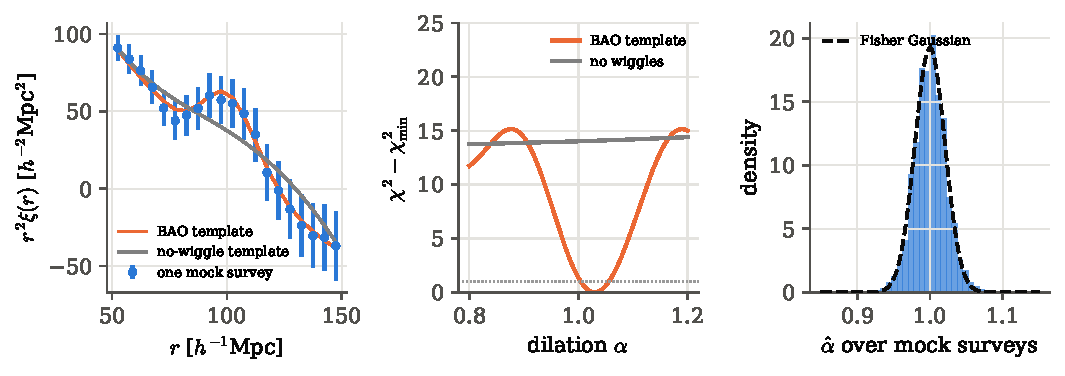
\includegraphics[width=\linewidth]{figures/chT2/bao_fit.pdf}
\caption{Fitting the BAO dilation. Left: one mock correlation function (times $r^2$, with the diagonal errors) and the best fits of the BAO template and of the no-wiggle template. Middle: the profile $\chi^2(\alpha)$ for both; the BAO template has a clear minimum near $\alpha=1$, the no-wiggle one is flat and higher. Right: the distribution of $\hat\alpha$ over the mock surveys and the Gaussian of the Fisher error; the tails are heavier than the Gaussian.}
\label{T2b:fig:bao-fit}
\end{figure}

Why the heavier tails? In a mock where noise happens to weaken the bump, $\chi^2(\alpha)$ is shallow and can have a second minimum where a noise wiggle lines up with the template. The likelihood is then far from Gaussian in $\alpha$, and the curvature at the minimum underestimates the real spread. At a $4\sigma$ detection this happens often; at the $10$--$20\sigma$ of a DESI bin it does not, and DESI finds its posteriors ``well approximated by Gaussian distributions'' \cite[Sec.~2.3.2]{DESI2024VI}.

\begin{inpractice}[Verification versus research]
Here the mocks \emph{verify} the analysis: we know $\alpha=1$, and we check that the estimator is unbiased and that its error bar covers the truth at the stated rate. In research the same machinery is the \emph{instrument}. DESI estimates the covariance of $\hat\xi$ from large sets of mock catalogues and analytic models, because the real survey has a mask, varying completeness and non-linear clustering that \eqref{T2b:eq:xi-cov} ignores; it calibrates the reconstruction and the theoretical systematics (below $0.1$--$0.2\%$) on simulations; and it blinds the data, shifting the BAO position in the catalogues until the pipeline is frozen \cite[Sec.~2.3.1]{DESI2024VI}. A full analysis uses thousands of mocks; ours uses $\TwbaoNmock$ Gaussian draws from an analytic covariance and no reconstruction.
\end{inpractice}

\subsection{What DESI's distances say}

\paragraph{Their question.} DESI measured the ruler at seven redshifts in its first year. The question we reproduce is: \emph{do the BAO distances alone, with no CMB and no supernovae, fix the matter density $\Omega_m$ and the expansion scale $H_0r_d$ in flat $\Lambda$CDM, and do they agree with the $\Lambda$CDM that fits the CMB?} It matters because the ruler is calibrated by early-universe physics and read at $z<2.5$, a test of the model across most of cosmic time.

\paragraph{Their data.} Each bin gives $D_M/r_d$ and $D_H/r_d$ with their correlation coefficient where the signal is strong, and $D_V/r_d$ alone for the bright galaxies (BGS) and the quasars (QSO), where it is weak \cite[Table~1]{DESI2024VI}:
\begin{center}
\small
\begin{tabular}{@{}lccccc@{}}
\toprule
tracer & $z_{\rm eff}$ & $D_M/r_d$ & $D_H/r_d$ & $D_V/r_d$ & correlation\\
\midrule
BGS & $0.295$ & -- & -- & $7.93\pm0.15$ & --\\
LRG & $0.510$ & $13.62\pm0.25$ & $20.98\pm0.61$ & -- & $-0.445$\\
LRG & $0.706$ & $16.85\pm0.32$ & $20.08\pm0.60$ & -- & $-0.420$\\
LRG+ELG & $0.930$ & $21.71\pm0.28$ & $17.88\pm0.35$ & -- & $-0.389$\\
ELG & $1.317$ & $27.79\pm0.69$ & $13.82\pm0.42$ & -- & $-0.444$\\
QSO & $1.491$ & -- & -- & $26.07\pm0.67$ & --\\
Ly$\alpha$ & $2.330$ & $39.71\pm0.94$ & $8.52\pm0.17$ & -- & $-0.477$\\
\bottomrule
\end{tabular}
\end{center}
Five bins with two numbers and two bins with one make $5\times2+2=\TwdNdata$ numbers. The correlation is negative because the data pin down the overall size of the ring better than its shape: a fit that stretches the ring across the line of sight compensates by shrinking it along the line of sight.

\paragraph{The model, derived.} In flat $\Lambda$CDM at these redshifts (radiation is $0.1\%$ of $H^2$ even at $z=2.3$) the predictions are
\begin{equation}
  \frac{D_H}{r_d}(z)=\frac{c}{H_0r_d}\,\frac{1}{E(z)},\qquad
  \frac{D_M}{r_d}(z)=\frac{c}{H_0r_d}\int_0^z\frac{\dd z'}{E(z')},\qquad
  E(z)=\sqrt{\Omega_m(1+z)^3+1-\Omega_m}.
  \label{T2b:eq:bao-lcdm}
\end{equation}
Only two numbers appear: $\Omega_m$, which sets how the distances change with redshift, and the product $H_0r_d$, which sets their overall scale. BAO alone therefore cannot separate $H_0$ from $r_d$.

\emph{Where we have met $H_0$ before.} The mock supernovae of \cref{3b:sec:hubble}, made with $H_0=70$, fixed only $M-5\log_{10}H_0$, and $H_0$ came out only once $M$ was supplied from outside. The ladder of \cref{T2b:sec:ladder} supplied it from parallaxes and Cepheids, and the real ladder gave $73.04\pm1.04$, $4.8\sigma$ above the CMB's $67.36\pm0.54$ (\cref{T2b:sec:tension}). The same degeneracy is back here with a ruler in place of the candle: the distances fix only the product $H_0r_d$, as the magnitudes fixed only $M-5\log_{10}H_0$, and the ruler's length plays the role of the candle's luminosity. Three things differ. The data are real DESI distances at $0.3<z<2.3$, far beyond the $z<0.15$ of the Hubble-flow supernovae, so $\Omega_m$ must be fitted alongside the scale rather than entering as the small $q_0$ correction. The calculation is a Bayesian posterior on a grid rather than a least-squares fit. And the calibration comes from the early Universe: $r_d$ is set by the sound waves before recombination, the same physics that fixes the CMB value of $H_0$ (\cref{10a:sec:cmb-planck}), not by geometry nearby. That is why the $H_0$ found below lands near the CMB value and not near the ladder's.

\paragraph{What we compute.} Each bin is a measurement $\bm d_b$ (two numbers or one) with Gaussian noise, and the model $\bm m_b(\Omega_m,hr_d)$ is \eqref{T2b:eq:bao-lcdm} evaluated at $z_{\rm eff}$ (with $D_V=(zD_M^2D_H)^{1/3}$ of \eqref{T2b:eq:dv} for the one-number bins). The bins are independent, so the $\chi^2$ is a sum over bins,
\begin{equation}
  \chi^2(\Omega_m,hr_d)=\sum_{b=1}^{7}\big(\bm d_b-\bm m_b\big)\T C_b^{-1}\big(\bm d_b-\bm m_b\big),
  \qquad
  C_b=\begin{pmatrix}\sigma_M^2&\rho\,\sigma_M\sigma_H\\ \rho\,\sigma_M\sigma_H&\sigma_H^2\end{pmatrix},
  \label{T2b:eq:desi-chi2}
\end{equation}
where $\sigma_M$ and $\sigma_H$ are the quoted errors of $D_M/r_d$ and $D_H/r_d$ and $\rho$ is their correlation; for a $D_V$ bin $C_b$ is just $\sigma_V^2$. The posterior with flat priors on a grid of $(\Omega_m,hr_d)$ is Bayes' theorem (\cref{ch:05}) with a constant prior:
\[
  p(\Omega_m,hr_d\given\bm d)=\frac{e^{-\chi^2(\Omega_m,hr_d)/2}}{\sum_{\rm grid}e^{-\chi^2/2}} ,
\]
and the means, standard deviations and correlation are sums over the grid weighted by it.

\paragraph{DESI and ours, side by side.} \Cref{T2b:fig:bao-desi} shows the distances and the posterior; the numbers are
\begin{center}
\small
\begin{tabular}{@{}lcc@{}}
\toprule
 & DESI \cite[eqs.~(4.1), (4.3)]{DESI2024VI} & ours\\
\midrule
$\Omega_m$ & $0.295\pm0.015$ & $\TwdOm\pm\TwdOmSd$\\
$h r_d$ [Mpc] & $101.8\pm1.3$ & $\TwdHrd\pm\TwdHrdSd$\\
$H_0$ [km/s/Mpc], with the CMB $r_d$ & $69.29\pm0.87$ & $\TwdHzero\pm\TwdHzeroErr$\\
\bottomrule
\end{tabular}
\end{center}
with correlation $\TwdCorr$ between our $\Omega_m$ and $hr_d$. The best fit has $\chi^2=\TwdChiMin$ for $\TwdNdata-2$ degrees of freedom, an ordinary value.

\paragraph{Why they differ, and by how much.} They barely do: the largest difference, $0.001$ in $\Omega_m$, is a fifteenth of the error bar. Three things could cause differences of that size. Our grid has steps of $0.001$ in $\Omega_m$ and $0.1$\,Mpc in $hr_d$, where DESI samples its posterior with MCMC. Our Gaussian is built from the errors and correlations as quoted in the table, rounded to two or three digits. And we neglect radiation, which changes $H^2$ by at most $0.1\%$ at the highest redshift, the Ly$\alpha$ bin, so $D_H$ by at most $0.05\%$, far below its $2\%$ error. For $H_0$, DESI also propagates the $0.2\%$ error of $r_d$, which we leave out; it is small next to the $1.3\%$ from $hr_d$.

\paragraph{Is Planck's $\Lambda$CDM consistent with it?} The Planck best fit ($h r_d=\TwdHrdP$\,Mpc) has $\chi^2=\TwdChiP$ against our minimum $\TwdChiMin$, so $\Delta\chi^2=21.1-12.8=8.3$. Under the hypothesis that the Planck point is the truth, $\Delta\chi^2$ between it and the best fit is a $\chi^2$ with two degrees of freedom, one per fitted parameter (Wilks' theorem, \cref{4a:sec:wilks}). Its tail is $\Prob(\chi^2_2>v)=e^{-v/2}$ (\eqref{10b:eq:rayleigh-tail}), so $p=e^{-8.3/2}=0.016$. Converted to the two-sided Gaussian language of the detection test, $2[1-\Phi(n)]=0.016$ gives $n=2.4\sigma$. That treats the Planck point as exact. DESI, including the errors of the CMB values, which spread the Planck point into its own small ellipse, quantifies the difference as a $1.9\sigma$ discrepancy ($1.6\sigma$ without CMB lensing) \cite[eq.~(4.2)]{DESI2024VI}: a mild tension, not a contradiction.

\paragraph{The lesson.} Twelve published numbers and a two-parameter grid are enough to recover DESI's headline constraint; what the grid cannot do on its own is separate $H_0$ from $r_d$, which is the subject of the next example.

\begin{figure}[htbp]
\centering
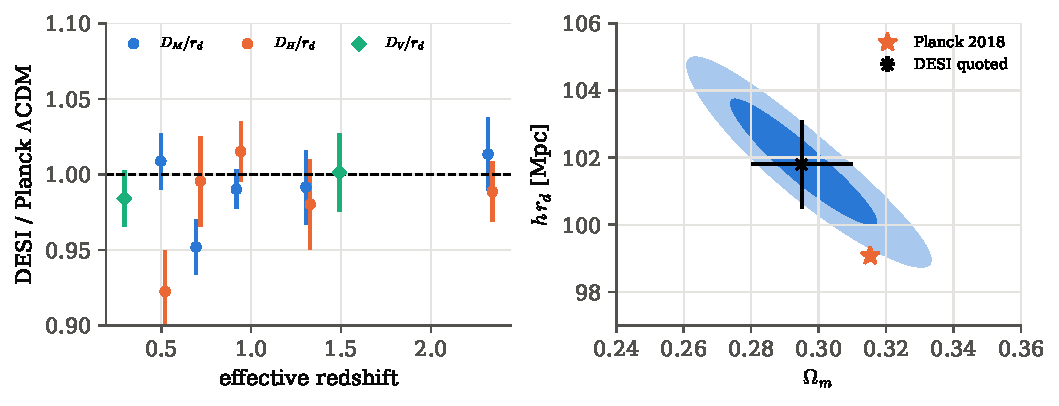
\includegraphics[width=0.95\linewidth]{figures/chT2/bao_desi.pdf}
\caption{Left: DESI DR1 BAO distances divided by the Planck $\Lambda$CDM prediction. Right: the $68\%$ and $95\%$ regions in $(\Omega_m,hr_d)$ from the twelve DESI numbers, computed on a grid, with DESI's quoted result (cross) and the Planck best fit (star). The long, tilted contour is the degeneracy of \eqref{T2b:eq:bao-lcdm}: a higher $\Omega_m$ can be traded for a lower $hr_d$.}
\label{T2b:fig:bao-desi}
\end{figure}

\paragraph{Example: the inverse distance ladder.} Take $r_d=147.09$\,Mpc from the CMB. Then $h=(h r_d)/r_d$, and the posterior above gives $H_0=\TwdHzero\pm\TwdHzeroErr$\,km/s/Mpc; DESI, propagating the small error of $r_d$ too, finds $69.29\pm0.87$, and $68.53\pm0.80$ with $r_d$ computed from a big-bang-nucleosynthesis value of $\omega_b$ instead of the CMB \cite[eqs.~(4.3)--(4.4)]{DESI2024VI}. This is a distance ladder run backwards, anchored at $z\approx1060$ by the physics of sound waves rather than at $z\approx0$ by parallaxes. It lands near the CMB value and well below the $73.04\pm1.04$ of the Cepheid ladder of \cref{T2b:sec:ladder}: the Hubble tension appears again when a ruler replaces a candle.

\paragraph{Where the statistics comes back in.} The estimator and covariance of $\hat\xi$ and $\hat P$ are \cref{ch:07}. The template fit is least squares with linear nuisances (\cref{ch:03}), the detection is a likelihood-ratio test (\cref{ch:04}), and the posterior on $(\Omega_m,hr_d)$ is the Bayesian grid of \cref{ch:05}, replaced by MCMC (\cref{ch:09}) when more parameters are free. The forecast precision of a BAO survey is a Fisher calculation (\cref{ch:10}), and galaxy clustering as cosmological data is \cref{ch:11}.
\section{Photometric redshifts and their error distributions}
\label{T2b:sec:photoz}

A spectrum gives a redshift to a part in ten thousand, but it costs a fibre and many minutes of a large telescope for each galaxy. Imaging surveys such as the ones used for weak lensing (\cref{ch:T1}) detect a billion galaxies, far too many and mostly too faint for spectra. What they have is the flux of each galaxy in five or six broad filters. That is enough for a rough redshift, because galaxy spectra have sharp features. The strongest in the optical is the break near $4000$\,\AA, where old stars and metal absorption make the light drop by a factor of two or three to the blue. At high redshift the Lyman series of intergalactic hydrogen removes the light blueward of $1216$\,\AA. As a galaxy is moved to higher redshift its spectrum slides to the red, and the break passes from one filter into the next (\cref{T2b:fig:photoz-sed}). The ratio of fluxes in neighbouring filters, a \newterm{colour}, therefore encodes the redshift. An estimate made this way is a \newterm{photometric redshift} (photo-$z$).

\paragraph{The question.} How is a redshift computed from a few fluxes, what is the distribution of its error, and how does that error propagate into the redshift distribution $n(z)$ of a sample, which is what cosmology actually uses?

\begin{figure}[htbp]
\centering
\begin{tikzpicture}
\begin{axis}[width=11cm,height=4.6cm,xmin=3000,xmax=11000,ymin=0,ymax=2.5,
  xlabel={observed wavelength [\AA]},ylabel={$f_\nu$ (arbitrary)},
  xtick={4000,6000,8000,10000},scaled x ticks=false,ytick=\empty,axis lines=left,
  every axis label/.style={font=\small},tick label style={font=\footnotesize}]
  \fill[black!7] (axis cs:3200,0) rectangle (axis cs:4000,2.5);
  \node[font=\footnotesize,text=softgray] at (axis cs:3600,2.3) {$u$};
  \fill[black!13] (axis cs:4000,0) rectangle (axis cs:5500,2.5);
  \node[font=\footnotesize,text=softgray] at (axis cs:4750,2.3) {$g$};
  \fill[black!7] (axis cs:5500,0) rectangle (axis cs:6900,2.5);
  \node[font=\footnotesize,text=softgray] at (axis cs:6200,2.3) {$r$};
  \fill[black!13] (axis cs:6900,0) rectangle (axis cs:8200,2.5);
  \node[font=\footnotesize,text=softgray] at (axis cs:7550,2.3) {$i$};
  \fill[black!7] (axis cs:8200,0) rectangle (axis cs:9200,2.5);
  \node[font=\footnotesize,text=softgray] at (axis cs:8700,2.3) {$z$};
  \fill[black!13] (axis cs:9200,0) rectangle (axis cs:10500,2.5);
  \node[font=\footnotesize,text=softgray] at (axis cs:9850,2.3) {$y$};
  \addplot[formblue,thick,domain=3000:11000,samples=400] {(x/(1.3*5000))^1.5*((x/1.3>4000)?1:0.35)};
  \addplot[bdryred,thick,domain=3000:11000,samples=400] {0.55*(x/(2.0*5000))^1.5*((x/2.0>4000)?1:0.35)};
  \node[font=\footnotesize,text=formblue,anchor=west] at (axis cs:9300,1.62) {$z=0.3$};
  \node[font=\footnotesize,text=bdryred,anchor=west] at (axis cs:9300,0.35) {$z=1.0$};
\end{axis}
\end{tikzpicture}
\caption{The same red-galaxy spectrum at two redshifts, seen through six broad filters (grey bands). At $z=0.3$ the $4000$\,\AA\ break lands at $5200$\,\AA, inside the $g$ band; at $z=1.0$ it has moved to $8000$\,\AA, inside the $i$ band. Which filter holds the break, and how deep the drop is, is what a photometric redshift reads.}
\label{T2b:fig:photoz-sed}
\end{figure}

\subsection{Template fitting as a likelihood}

\emph{What we observed} is a vector of fluxes $F_b$ in bands $b=1,\dots,6$, each with a Gaussian error $\sigma_b$. \emph{What could have produced it?} A galaxy of some spectral type $T$, at some redshift $z$, with some overall brightness $A$, predicting fluxes $A\,T_b(z)$, where $T_b(z)$ is the template spectrum redshifted to $z$ and integrated through filter $b$. \emph{How likely are the observed fluxes under each $(z,T)$?} The brightness is not of interest, so we integrate it out with a flat prior. The $\chi^2$ is quadratic in $A$, $\chi^2(A)=\chi^2_{\min}+(A-\hat A)^2S$ with $S=\sum_bT_b^2/\sigma_b^2$, so
\begin{align}
  \Like(z,T)
  &\eqby{1}\int\dd A\,\exp\Big[-\frac12\sum_b\frac{(F_b-AT_b)^2}{\sigma_b^2}\Big]
  \eqby{2}e^{-\chi^2_{\min}/2}\int\dd A\,e^{-S(A-\hat A)^2/2}
  \eqby{3}\sqrt{\frac{2\pi}{S}}\;e^{-\chi^2_{\min}(z,T)/2},\nonumber\\
  \chi^2_{\min}&\eqby{4}\sum_b\frac{F_b^2}{\sigma_b^2}-\frac{\big(\sum_bF_bT_b/\sigma_b^2\big)^2}{S},
  \qquad
  p(z\given\bm F)\propto n(z)\sum_T\Like(z,T).
  \label{T2b:eq:photoz-like}
\end{align}
\begin{explain}
  \item Independent Gaussian errors in each band; marginalise the nuisance amplitude (\cref{ch:05}).
  \item Expand the square in $A$ and complete it; $\hat A=\sum_bF_bT_b\sigma_b^{-2}/S$ is the least-squares amplitude.
  \item The Gaussian integral $\int e^{-Sx^2/2}\dd x=\sqrt{2\pi/S}$.
  \item Substitute $\hat A$ into $\chi^2$.
\end{explain}
The last expression is Bayes' theorem with the redshift distribution $n(z)$ of the population as the prior and the type summed over. The sum gives every template the same weight: it is a flat prior over the types, even though the population the experiment below draws from is $35\%$ red and $65\%$ blue. A type prior would multiply each $\Like(z,T)$ by the fraction of galaxies of type $T$. The photo-$z$ is then usually the peak of $p(z\given\bm F)$, but the whole posterior is the honest answer.

\subsection{The error distribution}

The error $z_{\rm phot}-z$ is not a Gaussian. It has a Gaussian-looking core whose width grows with redshift as $\sigma_z\propto1+z$. Why? A feature at rest wavelength $\lambda_{\rm rest}$ is observed at $\lambda_{\rm obs}=(1+z)\lambda_{\rm rest}$, so $\delta(1+z)/(1+z)=\delta\lambda_{\rm obs}/\lambda_{\rm obs}$. Broad filters locate the break only to a fixed fraction of the wavelength (a filter's width is roughly proportional to its central wavelength), so $\delta\lambda_{\rm obs}/\lambda_{\rm obs}$ is about constant, and then $\sigma_z=\delta z$ is a constant times $1+z$. Good surveys reach $\sigma_z/(1+z)\approx0.02$--$0.05$. And it has \newterm{catastrophic outliers} with $|z_{\rm phot}-z|\sim1$. The main cause is a degeneracy: a sharp drop observed at a wavelength $\lambda_{\rm obs}$ may be the $4000$\,\AA\ break of a nearby galaxy or the Lyman-$\alpha$ edge of a distant one, $(1+z_{\rm low})\,4000\,\text{\AA}=(1+z_{\rm high})\,1216\,\text{\AA}$. For $z_{\rm low}=0.16$,
\[
  1+z_{\rm high}=1.16\times\frac{4000}{1216}=3.82,\qquad z_{\rm high}=2.8 ,
\]
so a galaxy at $z_{\rm high}=2.8$ can be mistaken for one at $z_{\rm low}=0.16$ \cite[p.~96]{Weinberg2013}. Filters on both sides of both features, from $u$ to the near infrared, break the degeneracy.

Weinberg et al.\ describe the error by the joint distribution $P(z_p,z)$ of photo-$z$ and true redshift, and summarise it by the conditional bias and scatter $\delta z(z_p)=z_p-\langle z\rangle_{z_p}$ and $\sigma_z(z_p)$ \cite[p.~94, eq.~(100)]{Weinberg2013}. They then make a point that is pure Bayes: $P(z\given z_p)=P(z)\,P(z_p\given z)/P(z_p)$ \cite[eq.~(101)]{Weinberg2013}, so a photo-$z$ that is unbiased in the sense $\langle z_p\rangle_z=z$ can still have $\delta z(z_p)\ne0$.

A picture makes the reason plain (\cref{5a:sec:reallocation}). Think of each true redshift $z$ as an urn, and of the photo-$z$ as a ball drawn from it: the urn at $z$ gives out balls spread around $z$, with $P(z_p\given z)$ saying how readily it gives the ball labelled $z_p$. The population $n(z)$ says how many urns of each kind there are. We are handed one ball, labelled $z_p$, and asked which urn it came from. Two things decide: how readily each kind of urn gives this ball, and how many urns of that kind there are. Where urns are plentiful, even a modest chance per urn adds up to many balls labelled $z_p$, so the answer is pulled towards the crowded side. The ball tells us about its urn; it does not change the urns. This is the shrinking sample space once more: knowing the label $z_p$ discards every draw with a different label, and what survives is weighted by the number of urns that produced it (\cref{5a:sec:shrink}). It is the same structure as the Malmquist calculation of \cref{T2b:sec:malmquist}, where the urns were absolute magnitudes and their number was set by the volume. How large is the difference? Take a Gaussian error, $P(z_p\given z)=\Normal(z_p;z,\sigma^2)$, and a population whose number rises locally as $P(z)\propto e^{sz}$. Then
\begin{align}
  P(z\given z_p)
  &\eqby{1}\propto e^{sz}\exp\Big[-\frac{(z-z_p)^2}{2\sigma^2}\Big]
  \eqby{2}\propto\exp\Big[-\frac{(z-z_p-s\sigma^2)^2}{2\sigma^2}\Big],
  \qquad
  \langle z\rangle_{z_p}\eqby{3}z_p+s\sigma^2 .
  \label{T2b:eq:photoz-bayes}
\end{align}
\begin{explain}
  \item Bayes' theorem; $P(z_p)$ does not depend on $z$.
  \item Complete the square, exactly as in the Malmquist calculation \eqref{T2b:eq:malmquist}.
  \item The mean of the Gaussian.
\end{explain}
Where $n(z)$ rises, galaxies observed at $z_p$ are more likely to have scattered \emph{up} from below, since there were more of them below; where it falls, the opposite. It is the Malmquist bias of \cref{T2b:sec:malmquist} with redshift in place of magnitude: the population we draw from reweights the measurement.

\paragraph{Why the mean of $n(z)$ is the number that matters.} A weak-lensing analysis bins galaxies by photo-$z$ and needs the true $n(z)$ of each bin. The lensing signal depends mostly on its mean redshift. A lens bends the light of a source more the farther the source lies behind it (the lensing efficiency grows with the source distance, \cref{ch:T1}). So a bin whose mean is estimated too high predicts too much lensing for a given clustering amplitude; to match the observed shear, the fit lowers the amplitude, and $S_8$ comes out low \unpack{$S_8$ is the clustering amplitude that weak lensing constrains best}. Stage-III surveys need the mean redshift of each bin to about $0.01$, and Euclid and LSST need it $5$--$10$ times better \cite[Sec.~V.B.2]{Abdalla2022}. Outliers matter in proportion to their number. Suppose a fraction $f$ of a high-redshift bin are really foreground galaxies, in front of the lenses and so not lensed by them. The mean shear of the bin is then $(1-f)$ times the true one, and the shear power spectrum, which is quadratic in the shear, is $(1-f)^2\approx1-2f$ times. For $f=1\%$ that is $1\%$ and $2\%$ \cite[p.~94]{Weinberg2013}. Photometric redshifts can also be used for BAO, but only the transverse measurement survives, and only if $\sigma_z/(1+z)\lesssim4\%$ \cite[pp.~62--63]{Weinberg2013}. The line-of-sight measurement is lost much earlier. A redshift error equivalent to a velocity $\sigma_v$, that is $\sigma_z=(1+z)\sigma_v/c$, smears positions along the line of sight by $c\sigma_z/H(z)=(1+z)\sigma_v/H(z)$. For $\sigma_v=1000$\,km/s at $z=1$, with $H(1)\approx120$\,km/s/Mpc, that is $2\times1000/120\approx17$\,Mpc, comparable to or larger than the width of the acoustic bump, so its radial position, and with it $H(z)$, is erased \cite[pp.~62--63]{Weinberg2013}. The distribution $P(z\given z_p)$ is calibrated with spectroscopic subsamples ($10^5$ spectra for Stage IV) or with the angular cross-correlation of photometric galaxies with a spectroscopic survey. Why does the cross-correlation measure $P(z\given z_p)$? Both samples trace the same matter, $\delta_{\rm spec}=b_{\rm spec}\delta$ and $\delta_{\rm phot}=b_{\rm phot}\delta$ (\cref{T2b:sec:tracers}). Galaxies at different true redshifts are too far apart to be correlated, so the photometric galaxies selected by $z_p$ correlate with a thin spectroscopic slice at $z$ only through the fraction of them that really sit at $z$. Their cross-correlation is therefore $b_{\rm spec}\,b_{\rm phot}\,P(z\given z_p)$ times the matter correlation at $z$ \cite[p.~97]{Weinberg2013}: the bias of \cref{T2b:sec:tracers} returns as a nuisance.

\paragraph{The experiment.} \pyname{11_photoz.py} builds a mock imaging survey:
\begin{center}
\small
\begin{tabularx}{\linewidth}{@{}l>{\raggedright\arraybackslash}X>{\raggedright\arraybackslash}X@{}}
\toprule
ingredient & choice & why\\
\midrule
galaxies & $\TwpN$, from $n(z)\propto z^2e^{-(z/\TwpZzero)^{1.5}}$ & a typical deep-imaging redshift distribution\\
types & $35\%$ red, $65\%$ blue & two templates, strong and weak $4000$\,\AA\ break\\
spectra & power law, $4000$\,\AA\ break, Lyman absorption & the features a photo-$z$ reads\\
mismatch & each galaxy's slope and break differ a little & templates are never exactly right\\
filters & six top-hats, $u$ to $y$ (\cref{T2b:fig:photoz-sed}) & broad bands\\
depths & $5\sigma$ limits $24.0$--$25.4$\,mag & realistic noise\\
redshift grid & $800$ values, $0<z<4$ & where \eqref{T2b:eq:photoz-like} is evaluated\\
\bottomrule
\end{tabularx}
\end{center}
It computes the six fluxes, adds noise, and evaluates \eqref{T2b:eq:photoz-like} on the grid:

\pyfile[firstline=65,lastline=86,firstnumber=65]{code/chT2/11_photoz.py}{The template likelihood, with the amplitude and the type marginalised, and the two posteriors}

\noindent Line 73 is $\chi^2_{\min}$ of \eqref{T2b:eq:photoz-like}, line 74 the width $\sqrt{1/S}$ of the amplitude integral, and line 76 the sum over types. Line 83 multiplies by the prior $n(z)$.

Two summary numbers describe the errors, both measured on $\Delta z\equiv(z_p-z)/(1+z)$, the error in the units in which it is roughly constant. A galaxy is an \newterm{outlier} if $|\Delta z|>0.15$, that is $|z_p-z|>0.15(1+z)$: an error far too large for the Gaussian core, typically a degeneracy. The width of the core is measured on the remaining galaxies by the \newterm{normalised median absolute deviation}, $\text{NMAD}=1.48\times\text{median}\,\big|\Delta z-\text{median}(\Delta z)\big|$. The median is used instead of the mean so that a few large errors cannot inflate it, and the factor $1.48$ makes it equal to $\sigma$ for a Gaussian (the median of $|x|$ for a unit Gaussian is $0.674=1/1.48$).

\emph{With a flat prior} the core width is $\text{NMAD}=\TwpNmadF$, and $\TwpOutF\%$ of the galaxies are outliers.

\emph{With the $n(z)$ prior}, the cause first. A degenerate galaxy has a likelihood with two peaks, one at low and one at high redshift. The prior multiplies each peak by the number of galaxies at that redshift, and $n(z)$ is far larger at $z\lesssim1$ than at $z\approx3$; so the peak on the poorly populated side is down-weighted, and when it was a spurious peak the error is removed. Then the size: the core barely changes ($\TwpNmadP$), but the outliers drop from $\TwpOutF\%$ to $\TwpOutP\%$. The price is paid by the rare galaxies that really sit on the poorly populated side: the high-redshift galaxy of \cref{T2b:fig:photoz} ($z=\TwpZb$) has a bimodal likelihood whose higher peak is right, and the prior moves it to the wrong, low-redshift peak, because the prior is doing exactly what it should for the typical galaxy with that colour, and this one is not typical.

\emph{The mean of a bin.} For the bin $\TwpBinLo<z_p<\TwpBinHi$ ($\TwpBinN$ galaxies) the true mean redshift is $\TwpMeanTrue$ and the mean photo-$z$ is $\TwpMeanZp$, an error of $0.01$, at the Stage-III requirement. Stacking the posteriors instead of the point estimates gives $\TwpMeanStack$, no better. Why no better? A posterior accounts for the photometric noise, but every posterior here is computed with the same two templates, and every real galaxy differs from its template in the same kind of way. That template mismatch shifts all the posteriors together, and averaging many of them cannot remove an error they share. The asymmetry of \eqref{T2b:eq:photoz-bayes} is visible where $n(z)$ is steep: at $z=\TwpCondZlow$, on the rising side, $\langle z_p\rangle_z=\TwpCondAlow$ but $\langle z\rangle_{z_p}=\TwpCondBlow$; at $z=\TwpCondZ$, on the falling side, $\TwpCondA$ against $\TwpCondB$.

\begin{figure}[htbp]
\centering
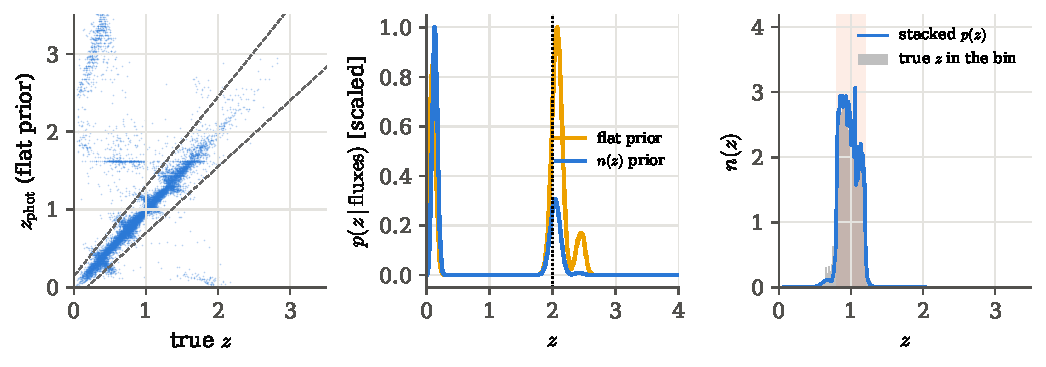
\includegraphics[width=\linewidth]{figures/chT2/photoz.pdf}
\caption{Left: photo-$z$ against true redshift (flat prior); the dashed lines bound the core $|z_p-z|<0.15(1+z)$, and the clumps outside are the degeneracies. Middle: the redshift posterior of one galaxy at $z=2.0$ (dotted line) with a flat prior and with the $n(z)$ prior. Right: the true redshifts of the galaxies selected by $0.8<z_p<1.2$ (grey) and the sum of their posteriors (blue).}
\label{T2b:fig:photoz}
\end{figure}

\paragraph{Nerfed, honestly.} Two toy templates, top-hat filters and a population independent of magnitude make the experiment run in a second. Real pipelines use hundreds of templates or machine-learning estimators trained on spectroscopic samples, fold in magnitude-dependent priors, and calibrate $n(z)$ per bin with spectroscopic subsamples, clustering redshifts and self-organising maps of colour space; the residual uncertainty of each bin's mean is then carried as a nuisance parameter.

\paragraph{Where the statistics comes back in.} The photo-$z$ posterior is Bayes' theorem with a nuisance amplitude marginalised (\cref{ch:05}). The core-plus-outliers error distribution is a mixture model, fitted with the likelihood methods of \cref{ch:03}. The shift of the mean of each bin is the nuisance parameter that weak-lensing likelihoods marginalise (\cref{ch:T1}), sampled with MCMC (\cref{ch:09}), and its required accuracy is set by a Fisher forecast (\cref{ch:10}).
\paragraph{Where each item is used.}
The standardised supernova distance \eqref{T2b:eq:tripp} with the noise budget \eqref{T2b:eq:mu-pec} is the datum of the $H_0$ problem of \cref{ch:03} and of every supernova likelihood after it. The ladder \eqref{T2b:eq:gls} is a worked generalised least-squares fit whose covariance is the inverse Fisher matrix of \cref{ch:10}. The selection-aware likelihood \eqref{T2b:eq:trunc-like} is the template for any analysis of a selected sample. The bias, shot noise and Kaiser factor \eqref{T2b:eq:threshold-bias}--\eqref{T2b:eq:kaiser} turn the matter $P(k)$ of \cref{ch:07} into the galaxy $P_g(k,\mu)$ that \cref{ch:11} fits. The BAO distances \eqref{T2b:eq:dv} and \eqref{T2b:eq:bao-lcdm} are a compact, nearly Gaussian likelihood used with the samplers of \cref{ch:09}. And the photo-$z$ posterior \eqref{T2b:eq:photoz-like} and its mean-redshift bias are the redshift nuisances of the weak-lensing likelihoods of \cref{ch:T1}.

\begin{recap}
\begin{itemize}[itemsep=1pt]
  \item Type~Ia supernovae are standardisable: $\mu=m_B-M+\alpha x_1-\beta c$ reduces a $0.4$\,mag scatter to $\approx0.12$\,mag, a $6\%$ distance per supernova; noisy colours dilute the fitted $\beta$ by $V_c/(V_c+\sigma_c^2)$, and peculiar velocities add $2.17\,\sigma_v/cz$\,mag.
  \item Supernovae measure only $M_B-5\log_{10}H_0$. The ladder (geometry $\to$ Cepheids or TRGB $\to$ calibrator supernovae $\to$ Hubble flow) is one linear model; each rung adds its variance, and lower-rung errors never average down.
  \item A flux limit biases a sample: $\langle M\rangle_{\rm det}=M_0-1.382\sigma^2$ in Euclidean space, $-\sigma\phi(t)/\Phi(t)$ near the limit; the cure is the likelihood of the selected data, $\Normal/\Phi(t)$.
  \item Galaxies trace matter with a bias, $\delta_g=b\delta$, $b=1+b_L$ with $b_L=\phi(\nu)/[\sigma(1-\Phi(\nu))]$ for threshold tracers; their power has shot noise $1/\bar n$; in redshift space $P_s=b^2(1+\beta\mu^2)^2P$, $\beta=f/b$.
  \item The BAO bump at $r_d\approx147$\,Mpc measures $D_M/r_d$ and $D_H/r_d$, or $D_V/r_d$; in flat $\Lambda$CDM DESI's distances fix $\Omega_m=0.295\pm0.015$ and $hr_d=101.8\pm1.3$\,Mpc, and with the CMB $r_d$ an inverse ladder gives $H_0\approx69$.
  \item Photometric redshifts have a core of width $\sim0.02(1+z)$ and catastrophic outliers from the Lyman/$4000$\,\AA\ degeneracy; $\langle z\rangle_{z_p}\ne z_p$ even when $\langle z_p\rangle_z=z$, and a bin's mean redshift must be known to $\lesssim0.01$.
\end{itemize}
\end{recap}

\section*{Chapter summary}
\addcontentsline{toc}{section}{Chapter summary}
\label{T2b:sec:summary}

Each astrophysical object of the chapter enters the statistics the same way: what is measured, where its noise lives, and which tool turns the measurement into physics.

\begin{center}
\small
\renewcommand{\arraystretch}{1.15}
\begin{tabularx}{\linewidth}{@{}>{\raggedright\arraybackslash}p{3.2cm}
                               >{\raggedright\arraybackslash}X
                               >{\raggedright\arraybackslash}p{2.4cm}@{}}
\toprule
\multicolumn{3}{@{}l}{\textbf{Compact binaries and gravitational waves}}\\
concept & operational meaning & used later in\\\midrule
chirp, chirp mass & $\dot f=\frac{96}{5}\pi^{8/3}(G\mathcal M/c^3)^{5/3}f^{11/3}$ from energy balance; only $\mathcal M=(m_1m_2)^{3/5}/M^{1/5}$ at leading order & \cref{ch:10}\\
stationary-phase waveform & $\tilde h=\mathcal Af^{-7/6}e^{-i\Psi(f)}$, $\dd^2\Psi/\dd f^2=2\pi/\dot f$: the signal model of the likelihood & \cref{ch:00,ch:05,ch:10}\\
LISA noise $S_n(f)$ & acceleration noise at low $f$, metrology and arm response at high $f$, Galactic foreground near a mHz; the covariance of Gaussian detector noise & \cref{ch:00,ch:10}\\
signal-to-noise ratio & $\rho^2=4\int|\tilde h|^2/S_n\,\dd f$; phase resolution $\sim1/\rho$ rad & \cref{ch:10}\\
dark-matter spike & $\rho\propto r^{-(9-2\gamma_i)/(4-\gamma_i)}$ around a growing black hole; fixes the physical meaning of the environmental parameter & \cref{ch:10}\\
power-law dephasing & extra power $\propto f^{-n}P_{\rm GW}$ gives $\delta\Psi=\beta u^{b}$, $b=-5/3-n$; one Fisher calculation per exponent & \cref{ch:09,ch:10}\\
\midrule
\multicolumn{3}{@{}l}{\textbf{Standard candles, distances and galaxy surveys}}\\
concept & operational meaning & used later in\\\midrule
Tripp standardisation & $\mu=m_B-M+\alpha x_1-\beta c$; Hubble residual Gaussian in magnitude, $\sigma\approx0.12$\,mag & \cref{ch:03,ch:05}\\
regression dilution & least squares with noisy regressors shrinks a slope by $V/(V+\sigma^2)$; cure: latent variables in a hierarchical model & \cref{ch:03,ch:05,ch:09}\\
distance ladder & one linear model through shared parameters $M_W$, $M_B$; covariance $(A\T\Cmat^{-1}A)^{-1}$; the $H_0$--$M_B$ degeneracy broken by geometry & \cref{ch:03,ch:04,ch:10}\\
Malmquist bias & detected candles brighter by $1.382\sigma^2$; near a limit $-\sigma\phi(t)/\Phi(t)$; likelihood of the selected data divides by $\Phi(t)$ & \cref{ch:03,ch:05,ch:06}\\
linear bias & $\delta_g=b\delta$, $P_g=b^2P$ on large scales; threshold and halo-model values; a nuisance in every clustering fit & \cref{ch:07,ch:11}\\
shot noise & $1/\bar n$ added to $P_g$; error $\sqrt{2/N_k}(1+1/\bar nP)$ per band; one-halo constant & \cref{ch:02,ch:07,ch:10}\\
Kaiser formula & $P_s(k,\mu)=b^2(1+\beta\mu^2)^2P$; monopole $1+\frac23\beta+\frac15\beta^2$; measures $f\sigma_8$ & \cref{ch:11}\\
BAO ruler & $\Delta\theta=r_d/D_M$, $\Delta z=r_d/D_H$, $D_V=(zD_M^2D_H)^{1/3}$; dilation $\alpha$ from a template fit with broadband nuisances & \cref{ch:04,ch:07,ch:09,ch:11}\\
DESI BAO likelihood & Gaussian in $(D_M/r_d,D_H/r_d)$ per bin; depends on $\Omega_m$ and $H_0r_d$ only; inverse ladder with $r_d$ & \cref{ch:05,ch:09}\\
photometric redshift & template likelihood with amplitude marginalised, times an $n(z)$ prior; core $\propto1+z$ plus outliers; $P(z\given z_p)$ by Bayes & \cref{ch:05,ch:T1}\\
mean-redshift nuisance & shift of each bin's $\langle z\rangle$, required to $\lesssim0.01$; marginalised in lensing likelihoods & \cref{ch:T1,ch:09,ch:10}\\
\bottomrule
\end{tabularx}
\end{center}

\subsection*{Reading the literature}

\begin{itemize}[leftmargin=1.2em,itemsep=2pt]
  \item \textbf{Inspirals and waveforms.} The quadrupole formula and the Newtonian chirp are in Maggiore's textbook \cite{Maggiore2007}; the stationary-phase waveform and the precision of the chirp mass in Cutler and Flanagan \cite{CutlerFlanagan1994}; parametrised deviations from general relativity in Yunes and Pretorius \cite{YunesPretorius2009}.
  \item \textbf{LISA.} The sensitivity curve and its ingredients in Robson, Cornish and Liu \cite{Robson2019}; the detector response and Doppler modulation in Barack and Cutler \cite{BarackCutler2004}.
  \item \textbf{Dark-matter environments.} Spikes around black holes from Gondolo and Silk \cite{GondoloSilk1999} and Sadeghian et al.\ \cite{Sadeghian2013}; dephasing of intermediate-mass-ratio inspirals in Eda et al.\ \cite{Eda2015}, with halo feedback in Coogan et al.\ \cite{Coogan2022} and relativistic corrections in Speeney et al.\ \cite{Speeney2022}; wave dark matter in Hui et al.\ \cite{HuiOstriker2017,HuiKabat2019}, Kim et al.\ \cite{Kim2023}, Chase et al.\ \cite{Chase2025} and Hancock and Witek \cite{HancockWitek2025}; the broader landscape of environmental effects in Barausse et al.\ \cite{Barausse2014}; dynamical friction in Chandrasekhar \cite{Chandrasekhar1943}; halo profiles in Navarro, Frenk and White \cite{NFW1996,NFW1997} and Correa et al.\ \cite{Correa2015}.
  \item \textbf{Cosmological distances.} Hogg's short note \cite{Hogg1999} defines every distance used here.
  \item \textbf{Probes of the expansion.} Weinberg et al.\ \cite{Weinberg2013} review supernovae (Sec.~3), BAO (Sec.~4) and weak lensing with photometric redshifts (Sec.~5.4.3), with their systematics.
  \item \textbf{Supernovae and the ladder.} The Pantheon+ compilation \cite{Brout2022PantheonPlus} and the SH0ES measurement \cite{Riess2022SH0ES}; the tensions and their proposed resolutions, with sections on ladder systematics and photometric redshifts, in Abdalla et al.\ \cite{Abdalla2022}; the CMB values in Planck 2018 \cite{Planck2018VI}.
  \item \textbf{Galaxy clustering.} The halo model and halo bias in Cooray and Sheth \cite{CooraySheth2002}; redshift-space distortions in Kaiser \cite{Kaiser1987}.
  \item \textbf{BAO.} The first detection in Eisenstein et al.\ \cite{Eisenstein2005}; the no-wiggle transfer function in Eisenstein and Hu \cite{EisensteinHu1998}; the DESI first-year cosmology in \cite{DESI2024VI}.
\end{itemize}
  